\documentclass[
    12pt, % Schriftgröße
    DIV=10,
    a4paper, % Papierformat
    oneside, % einseitiges Dokument
    titlepage, % es wird eine Titelseite verwendet
    parskip=half, % Abstand zwischen Absätzen (halbe Zeile)
    headings=normal, % Größe der Überschriften verkleinern
    listof=totoc, % Verzeichnisse im Inhaltsverzeichnis aufführen
    bibliography=totoc, % Literaturverzeichnis im Inhaltsverzeichnis aufführen
    captions=tableheading, % Beschriftung von Tabellen unterhalb ausgeben
    numbers=noendperiod 	% kein Punkt nach Nummerierung in Überschrift
]{scrreprt}

\usepackage[
    automark,       % Kapitelangaben in Kopfzeile automatisch erstellen
    headsepline,    % Trennlinie unter Kopfzeile
    footsepline,
    ilines          % Trennlinie linksbündig ausrichten
]{scrpage2}

\usepackage[ngerman]{babel}
\usepackage[utf8]{inputenc}
\usepackage[T1]{fontenc}
\usepackage[section]{placeins} % added by mwa
\usepackage{float} % added by mwa

\usepackage{setspace}
\onehalfspacing % Zeilenabstand 1,5 Zeilen

\usepackage{geometry}
\setlength{\topskip}{\ht\strutbox} % behebt Warnung von geometry
\geometry{left=35mm,right=30mm,top=25mm,bottom=45mm}

% Kopf- und Fußzeilen
\pagestyle{scrheadings}
% Kopf- und Fußzeile auch auf Kapitelanfangsseiten
\renewcommand*{\chapterpagestyle}{scrheadings} 
% Schriftform der Kopfzeile
\renewcommand{\headfont}{\normalfont}

% Kopfzeile
%\ihead{\large{\textsc{\titel}} \\[2ex] \textit{\headmark}}
\ihead{\large{} \\[2ex] \textit{\headmark}}
\chead{}
\ohead{
\includegraphics[scale=0.12]{\logo} \hspace*{25mm}}
\setlength{\headheight}{21mm} % Höhe der Kopfzeile
% Kopfzeile über den Text hinaus verbreitern
\setheadwidth[0pt]{textwithmarginpar} 
\setheadsepline[text]{0.4pt} % Trennlinie unter Kopfzeile

% Fußzeile
\ifoot{\autor}
\cfoot{}
\ofoot{\pagemark}

\usepackage{courier}
\usepackage{relsize} 
\usepackage[dvips,final]{graphicx}
\usepackage{amsmath,amsfonts}
\usepackage{longtable}
\usepackage{nameref}
\usepackage{mdframed} %mwa

% testing textbox



% end of testing textbox

\usepackage{eurosym}

\usepackage{booktabs}
\usepackage[table,xcdraw,dvipsnames]{xcolor}
\usepackage{rotating,tabularx}

\usepackage{tablefootnote}

\usepackage{hhline}
\usepackage{array}
\newcolumntype{C}[1]{>{\centering\let\newline\\\arraybackslash\hspace{0pt}}m{#1}}   % center
\newcolumntype{L}[1]{>{\raggedright\let\newline\\\arraybackslash\hspace{0pt}}m{#1}} % left
\newcolumntype{R}[1]{>{\raggedleft\let\newline\\\arraybackslash\hspace{0pt}}m{#1}}  % right
\newcolumntype{w}[1]{>{\raggedleft\hspace{0pt}}p{#1}}


\usepackage{paralist} % Formatierung von Listen ändern
\usepackage{todonotes}

% usage: \todod{Adressat}{Frage}    -> Wenn das erste Feld mit einem der definierten Strings befüllt ist, ändert sich automatisch die Farbe. Auf diese Weise kann z.B. der Betreuer oder der Professor direkt sehen, wo Fragen an ihn gerichtet sind
\newcommand{\mytodo}[2]{
    \IfEqCase{#1}{
        {Betreuer}{\todo[color=orange]{#1}{\textit{#2}}}
        {Prof. XY}{\todo[color=yellow]{#1}{\textit{#2}}}
        {cite}{\todo[color=blue]{#1}{}}
        {}{\todo[color=green]{#1}{\textit{#2}}}
    }[\PackageError{mytodo}{Undefined option to todod: #1}{}]
}


\usepackage[printonlyused]{acronym}

\usepackage{chronology}
\usepackage{tikz}
%\usetikzlibrary{shapes,snakes} % mwa testing textbox
\usepackage{pgfplots}
\usepackage{numprint}
\pgfplotsset{compat=1.14} 
\usepackage{mathptmx}
\usepackage{calc}
\usepackage{xcolor} 
%\usepackage[usenames,dvipsnames]{xcolor}

%import datatool for reading data from .csv file
\usepackage{datatool}
\usepackage[utf8]{inputenc}
\DTLsetseparator{;}
\DTLloaddb[keys={kriterium,wert}]{valuesTestEssen}{bilder/data/CsvValuesTestEssen.csv}  % csv Werte Testessen
\DTLloaddb[keys={kriterium,wert}]{valuesUserTest}{bilder/data/CsvValuesUserTest.csv}% csv Werte User TEst

\usepackage[toc]{glossaries}
%\loadglsentries{nebenkapitel/Glossar}
%\makeglossaries
\glsaddall{}

\usepackage{pifont}
\newcommand{\cmark}{\textcolor[rgb]{0,0.6,0}{\ding{51}}}
\newcommand{\xmark}{\textcolor{red}{\ding{55}}}

\newcommand*{\TakeFourierOrnament}[1]{{\fontencoding{U}\fontfamily{futs}\selectfont\char#1}}
\newcommand*{\danger}{\textcolor[RGB]{255,200,0}{\TakeFourierOrnament{66}}}

\frenchspacing % erzeugt ein wenig mehr Platz hinter einem Punkt

% Schusterjungen und Hurenkinder vermeiden
\clubpenalty = 10000
\widowpenalty = 10000 
\displaywidowpenalty = 10000

\usepackage{floatflt}

\usepackage{listings}
\definecolor{colBackground}{RGB}{240, 240, 240}
\definecolor{colKeys}{RGB}{0, 0, 255}
\definecolor{colIdentifier}{RGB}{0, 0, 0}
\definecolor{colComments}{RGB}{40, 220, 0}
\definecolor{colString}{RGB}{0, 150, 0}
\colorlet{punct}{red!60!black}
\definecolor{background}{HTML}{EEEEEE}
\definecolor{delim}{RGB}{20,105,176}
\colorlet{numb}{magenta!60!black}

\lstset{
    float=hbp,
    basicstyle=\ttfamily\color{black}\small\smaller,
    identifierstyle=\color{colIdentifier},
    keywordstyle=\color{colKeys},
    stringstyle=\color{colString},
    commentstyle=\color{colComments},
    columns=flexible,
    tabsize=2,
    frame=single,
    extendedchars=true,
    showspaces=false,
    showstringspaces=false,
    numbers=left,
    numberstyle=\tiny,
    numbersep=5pt,
    breaklines=true,
    backgroundcolor=\color{colBackground},
    emph={square}, 
    emphstyle=\color{red}, 
    emph={[2]root,base}, 
    emphstyle={[2]\color{blue}},
    breakautoindent=true
}

\lstdefinelanguage{myjson}{
    literate=
     *{0}{{{\color{numb}0}}}{1}
      {1}{{{\color{numb}1}}}{1}
      {2}{{{\color{numb}2}}}{1}
      {3}{{{\color{numb}3}}}{1}
      {4}{{{\color{numb}4}}}{1}
      {5}{{{\color{numb}5}}}{1}
      {6}{{{\color{numb}6}}}{1}
      {7}{{{\color{numb}7}}}{1}
      {8}{{{\color{numb}8}}}{1}
      {9}{{{\color{numb}9}}}{1}
      {:}{{{\color{punct}{:}}}}{1}
      {,}{{{\color{punct}{,}}}}{1}
      {\{}{{{\color{delim}{\{}}}}{1}
      {\}}{{{\color{delim}{\}}}}}{1}
      {[}{{{\color{delim}{[}}}}{1}
      {]}{{{\color{delim}{]}}}}{1},
}

\usepackage[
    %draft=false,    % added by mwa
    bookmarks,
    bookmarksopen=true,
    colorlinks=true,
    linkcolor=black,
    anchorcolor=black,
    citecolor=black,
    filecolor=black,
    menucolor=black,
    urlcolor=black, 
    %backref,
    plainpages=false,
    pdfpagelabels,
    hypertexnames=false
]{hyperref}

%\hypersetup{final} % added by mwa
\usepackage{url} % added by mwa, allow line breaks of url in biliography
\def\UrlBreaks{\do\/\do-} % added by mwa, allow line breaks of url in biliography

% Abkürzungen mit korrektem Leerraum 
\newcommand{\ua}{\mbox{u.\,a.\ }}
\newcommand{\zB}{\mbox{z.\,B.\ }}
\newcommand{\vgl}{vgl.\ }
\newcommand{\bzw}{bzw.\ }
\newcommand{\evtl}{evtl.\ }
\newcommand{\ggf}{ggf.\ }
\newcommand{\idR}{i.\,d.\,R.\ }

\newcommand{\bs}{$\backslash$}
\newcommand{\arrow}{$\to$}

% Listenelement mit fetter Überschrift und Zeilenumbruch -> \itemd{Überschrift}
\newcommand{\itemd}[1]{\item{\textbf{#1}}\\}

\newcommand{\textcour}[1]{
    \begin{footnotesize}
        \texttt{#1} 
    \end{footnotesize}
}

% Tabelleninhalte werden grundsätzlich in kleinerer Schriftgröße erstellt
\usepackage{etoolbox}
\AtBeginEnvironment{tabular}{\footnotesize}



\newcommand{\titel}{Konzeption und Implementierung einer Android Applikation zur Raumbuchung via Conversational User Interface}
\newcommand{\art}{Masterarbeit}
\newcommand{\fachgebiet}{Software-Engineering}
\newcommand{\autor}{Michael Wagner}
\newcommand{\fakultaet}{Elektrotechnik Feinwerktechnik Informationstechnik}
\newcommand{\studienbereich}{Elektronische und Mechatronische Systeme}
\newcommand{\vertiefung}{Informationstechnik}
\newcommand{\matrikelnr}{2560795}
\newcommand{\erstgutachter}{Prof. Dr. Oliver Hofmann}
\newcommand{\zweitgutachter}{Prof. Dr. Hans-Georg Hopf}
\newcommand{\betreuer}{Dipl.-Inf. Steffen Blümm}
\newcommand{\jahr}{2018}
\newcommand{\ort}{Nürnberg}
\newcommand{\logo}{bilder/LogoOhmHochschule.jpg}
\newcommand{\hs}{Technische Hochschule Nürnberg Georg Simon Ohm}
\newcommand{\adorsys}{adorsys GmbH \& Co. KG}

\begin{document}

% auch subsubsection nummerieren
\setcounter{secnumdepth}{3}
\setcounter{tocdepth}{3}

% Deckblatt und Abstract ohne Seitenzahl
\ofoot{}

% added by mwa
% first page - clear page
\clearpage
\thispagestyle{empty}
\hfill
\clearpage

\thispagestyle{plain}
\begin{titlepage}

\begin{center}
    
\includegraphics[scale=1.1]{bilder/LogoTHMitText.jpeg}\\[11ex]  
    
    \huge{\textbf{\titel}}\\[6.5ex] 
    \LARGE{\textbf{\art}}\\[1.5ex]
    
    \normalsize
    \begin{tabular}{w{5.4cm}p{8cm}}\\
    vorgelegt von:  & \quad \textbf{\autor}\\[1.2ex]
    Fakultät: & \quad \fakultaet\\[1.2ex]
    Studiengang: & \quad \studienbereich\\[1.2ex]
    Vertiefungsrichtung: & \quad \vertiefung\\[1.2ex]
    Erstgutachter:  & \quad \erstgutachter\\[1.2ex]
    Zweitgutachter: & \quad \zweitgutachter\\[1.2ex]
    Betreuer: & \quad \betreuer\\[3ex]
    \end{tabular}
    
    WiSe 2018/2019\\[6ex]
    Schlagworte: Conversational User Interface, Chatbot, Android, Dialogflow, Node.js
\end{center}
\end{titlepage}

%\section*{Zusammenfassung}
%\label{sec:zusammenfassung}

\section*{Abstract}
\label{sec:abstract}

Bei der Verwendung eines Conversational User Interface (CUI) bedient der Nutzer ein System über geschriebene und gesprochene Sprache. Anders als bei einem Graphical User Interface (GUI) muss die Antwort auf eine Frage nicht mehr gesucht, sondern kann direkt erfragt werden. Nachdem das System auf natürliche Art und Weise mit dem Nutzer interagiert, versteht es idealerweise alle Variationen einer Anfrage. Unabhängig davon, wie diese im Einzelnen formuliert sind. \\
Im Rahmen dieser Arbeit liegt der Fokus auf der Entwicklung eines Chatbots, also eines textbasierten CUIs. Die Arbeit umfasst die Konzeption und Implementierung eines solchen Systems im Kontext einer Raumbuchung. Dazu werden zunächst die Anforderungen an ein CUI im Allgemeinen und anschließend in Bezug auf ein Raumbuchungssystem betrachtet. In diesem Zusammenhang werden Methoden und Techniken aus dem Bereich Usability Engineering angewendet. Die Idee ist hierbei, multimodal mit dem CUI zu interagieren. So können GUI-Elemente wie beispielsweise Buttons oder Slider in die Konversation mit einfließen. Der Nutzer soll dabei jederzeit die Möglichkeit haben, auch textuelle Nachrichten an den Chatbot zu senden. Diese Ansätze werden mit Hilfe eines prototypischen Systems umgesetzt, überprüft und evaluiert. Durch die Umsetzung einiger der prototypisch erprobten Ansätze ist der Nutzer schließlich in der Lage, mit Hilfe eines Chatbots auf Basis einer Android Applikation nach freien Räumen zu suchen und einen Besprechungsraum zu reservieren.
\ofoot{\pagemark}

\pagenumbering{Roman}
\tableofcontents            % Inhaltsverzeichnis

\chapter*{Abkürzungsverzeichnis}			% keine Kapitelnummer -> section*
\addcontentsline{toc}{chapter}{Abkürzungsverzeichnis}
\markboth{Abkürzungsverzeichnis}{Abkürzungsverzeichnis}

\begin{acronym}[Bash]
	
	%%% A - E %%%
	\acro{AI}{Artificial Intelligence}
	\acro{ANN}{Artificial Neural Network}
	\acro{API}{Application Programming Interface}
	\acro{ASR}{Automatic Speech Recognition}
	
	\acro{CLI}{Command Line Interface}
	\acro{cpt}{conversation prototyping tool}
	\acro{CUI}{Conversational User Interface}
	
	\acro{DL}{Deep Learning}
	\acro{DM}{Dialog Management}
	\acro{dp}{density-independent pixel}
    
    %%% F - J %%%
    \acro{GUI}{Graphical User Interface}
    
    \acro{HCI}{Human Computer Interaction}
    \acro{HR}{Human Resources}
    \acro{HTML}{Hypertext Markup Language}
    \acro{HTTP}{Hypertext Transfer Protocol}
    
    \acro{ID}{Identifier}
    
    \acro{JS}{JavaScript}
    \acro{JSON}{JavaScript Object Notation}
    \acro{JVM}{Java Virtual Machine}
	
	%%% K - O %%%
	\acro{KI}{Künstliche Intelligenz}
	
	\acro{ML}{Machine Learning}
	\acro{MS-DOS}{Microsoft Disk Operating System}
	
	\acro{NLP}{Natural Language Processing}
	\acro{NLU}{Natural Language Understanding}
	\acro{NoSQL}{Not only Structured Query Language}
	\acro{npm}{Node Package Manager}
	
	
	%%% P - T %%%
	\acro{REST}{Representational State Transfer}
	
	\acro{SDK}{Software Development Kit}
	\acro{SQL}{Structured Query Language}
	
	\acro{TTS}{Text To Speech}
	
	
	%%% U - Z %%%
	
	\acro{UI}{User Interface}
	\acro{URL}{Uniform Resource Locator}
	\acro{UCD}{User Centered Design}
	\acro{UX}{User Experience}
	
	\acro{WOz}{Wizard of Oz}
	
	\acro{XML}{Extensible Markup Language}
	
    
\end{acronym}

\clearpage
      % Abkürzungsverzeichnis
%\clearpage\markboth{\nomname}{\nomname} % für korrekte Überschrift in der Kopfzeile
%\printnomenclature

\listoffigures              % Abbildungsverzeichnis
\listoftables               % Tabellenverzeichnis

\renewcommand{\lstlistlistingname}{Quellcodeverzeichnis}
\lstlistoflistings          % Quellcodeverzeichnis

\clearpage
\pagenumbering{arabic}

\chapter{Einleitung}
\label{cha:einleitung}

Dieses Kapitel spiegelt im Wesentlichen die Inhalte des im Vorfeld der Arbeit entstandenen Exposees wider. Wird bei bestimmten Begriffen, die sich auf Personengruppen beziehen, nur die männliche Form gewählt, so ist dies nicht geschlechtsspezifisch gemeint, sondern geschah ausschließlich aus Gründen der besseren Lesbarkeit. 

\section{Ausgangssituation}
\label{sec:ausgangssituation}

Bei der Verwendung eines \acp{CUI} bedient der Nutzer ein System durch schriftliche und mündliche Konversation \cite[S. 11]{mctear_conversational_2016}. Dabei beschreiben \acp{CUI} die Sprachverarbeitung und Kommunikation als Schnittstelle, unabhängig davon in welcher Modalität diese vorliegt. Es kann sich deshalb also sowohl um geschriebene als auch um gesprochene Sprache handeln. 

Eine wesentliche Herausforderung dabei ist es, den Nutzungskontext zu erschließen, diesen richtig zu interpretieren und eine passende Antwort zu geben. Die Textversionen der \acp{CUI} werden meist als Chatbots bezeichnet \cite[S. 1]{khan_build_2018}. Diese interaktiven Systeme mit teilweise künstlicher Intelligenz (\acs{KI}) bieten Funktionen an, welche unseren Alltag erleichtern sollen. Während also über ein \ac{GUI} die Antwort auf eine Frage gesucht werden muss, kann diese über ein \acl{CUI} einfach gestellt und direkt erfragt werden.

Mit diesem Hintergrund soll in dieser Masterarbeit die Möglichkeit einer Raumbuchung via \acl{CUI} umgesetzt werden. Heutzutage werden Raumreservierungen in nahezu allen Unternehmen mit Hilfe von Softwaresystemen wie Microsoft Outlook oder IBM Notes getätigt  \cite{foitzik_wie_2017}. Dabei lässt sich über ein \ac{GUI} zumeist eine Kalenderanwendung öffnen. Über diese kann dann nach verfügbaren Räumen gesucht, Einladungen verschickt oder die freien Zeiten der Teilnehmer geprüft werden.

\section{Ziel der Arbeit}
\label{sec:ziel-der-arbeit}

Das Ziel dieser Arbeit besteht darin, eine Android Applikation zur Raumreservierung via \acl{CUI} zu entwerfen. Dem Nutzer soll es möglich sein, einen Besprechungsraum mittels eines Chatbots zu reservieren. 

Das \ac{CUI} wird dabei durch Visualisierungen erweitert. So können \ac{GUI}-Elemente beispielsweise in Form von Buttons oder Slidern in die Konversation einfließen und diese erweitern. Der Nutzer soll dabei jederzeit die Möglichkeit haben, auch textuelle Nachrichten an den Chatbot zu senden. Im Gegensatz zur Bedienung einer rein grafischen Benutzeroberfläche sparen die Nutzer dabei Zeit \cite{weddehage_10_2016}, da das Suchen nach einem verfügbaren Raum vereinfacht wird. Anhand eines Prototypen kann dabei überprüft werden, wie schnell und effektiv eine Raumbuchung via \ac{CUI} stattfinden kann.

\section{Aufbau der Arbeit}
\label{sec:aufbau-der-arbeit}

Um dieses Ziel zu erreichen, wird die Vorgehensweise anhand der nachfolgenden Schritte genauer erläutert. Die grundsätzliche Anforderung dieser Arbeit ist bereits durch das Ziel beschrieben. Es geht prinzipiell darum ein Konzept zu erarbeiten, die Kommunikation zwischen den Komponenten zu klären und Nutzungskonzepte zu evaluieren. 

Durch das konkrete Thema sind bereits viele der Softwarekomponenten klar beschrieben. So wird es sich beispielsweise in jedem Fall um eine Android Applikation handeln. Da die \adorsys\ den Google-Kalender nutzt, würde sich hier die Verwendung des Chatbot-Builders Dialogflow anbieten. Zudem müssen Überlegungen hinsichtlich des Aufbaus der Konversationsstruktur und der Konversationsstrategie des Chatbots angestellt und evaluiert werden. Sämtliche Ergebnisse werden in dieser Arbeit zusammengefasst und bewertet.

\section{Projektträger}
\label{sec:projekttraeger}

Diese Masterarbeit wurde in Zusammenarbeit mit dem Unternehmen \adorsys\ durchgeführt. Um deren fachliche Kompetenzen und die Hintergründe, die zu dieser Arbeit geführt haben, besser einordnen zu können, wird das Unternehmen im Folgenden kurz vorgestellt.

Die \adorsys \, ist ein im Jahre 2006 in Nürnberg gegründetes, mittelständisches IT-Unternehmen. Es wird aktuell von dem Geschäftsgründer Francis Pouatcha Nouyeuwe und Stefan Hamm geleitet und beschäftigt derzeit 112 Mitarbeiter\footnote{Stand: 15. November 2018}  an den Standorten Nürnberg und Frankfurt am Main.

Fachlich hat sich die \adorsys \, auf individuelle Softwarelösungen für Kunden aus der Banken"~ und Versicherungsbranche spezialisiert. Mit dem Motto „Wir entwickeln Software für eine digitale Zukunft“ begleiten die eingesetzten Projektteams die Kunden von der ersten Idee bis hin zum fertigen Produkt. Dabei ist es unabhängig davon, ob eine bestehende Software modernisiert werden soll oder die Lösung zu einem neuen Geschäftsmodell fehlt. 

Selbst beschreibt sich das Unternehmen wie folgt:
\begin{quote}
    „Die adorsys ist ein seit 2006 bestehendes innovatives IT-Unternehmen für zielgenaue, individuelle und exklusive IT-Lösungen. Wir decken eine Vielzahl fachlicher und technologischer Themen ab und bieten die komplette Projektrealisierung aus einer Hand. Von Projektmanagement, Businessanalyse und Anforderungsentwicklung, Softwarearchitektur und -entwicklung über Development Services bis zur Betriebsvorbereitung.“ \cite{adorsys_gmbh_&_co._kg_company_2018}
\end{quote}

Das Unternehmen beschäftigt sich seit dem Aufkommen der neuen Generation von Sprachassistenten und Chatbots mit dem Thema Conversational User Interfaces. Im Rahmen von wissenschaftlichen Arbeiten werden derzeit Kompetenzen in diesem Bereich aufgebaut.
In Abbildung \ref{fig:logo-adorsys} ist das aktuelle Firmenlogo der \adorsys \, dargestellt.
\newline

\begin{figure}[htb]
    \centering
    
\includegraphics[width=0.6\textwidth]{bilder/logo.png}
    \caption{Logo der \adorsys \, \cite{adorsys_gmbh_&_co._kg_company_2018}}
    \label{fig:logo-adorsys}
\end{figure}

\section{Aufbau des Dokuments}
\label{sec:aufbau-des-dokuments}

Zur besseren Übersicht und Orientierung soll hier ein Überblick über die nachfolgenden Kapitel und deren Inhalte gegeben werden. 

\begin{enumerate}
  \item In der \nameref{cha:einleitung} wird in die Thematik eingeführt sowie auf die Ziele und den Aufbau der Arbeit eingegangen. Des Weiteren wird der Projektträger  \adorsys \ kurz vorgestellt. 
  
  \item Im Kapitel \nameref{cha:grundlagen} werden einige für die Masterarbeit notwendigen Begrifflichkeiten, Technologien und Funktionsweisen beschrieben. Dabei wird verstärkt auf Conversational User Interfaces und Android Applikationen eingegangen. 
  
  \item Das Kapitel \nameref{cha:konzeption} befasst sich mit dem Requirements Engineering und der prototypischen Umsetzung des Systems. Dabei werden Nutzeranforderungen im Kontext des Usability Engineering analysiert und bewertet. 
  
  \item Im Kapitel \nameref{cha:implementierung} werden die für die Umsetzung benötigten Komponenten ausgewählt, deren Kommunikation und Schnittstellen geklärt sowie einige Anmerkungen zur Implementierung gegeben.
  
  \item In der \nameref{cha:schlussbetrachtung} werden die Ergebnisse der Arbeit in Form eines Fazits und Ausblicks zusammengefasst.
  
  \item Im \nameref{sec:Anhang} sind alle Ausarbeitungen in vollständiger Form dargestellt. Zusätzlich ist die Struktur der beiliegenden CD beschrieben.
\end{enumerate}

\chapter{Grundlagen}
\label{cha:grundlagen}

In diesem Kapitel werden verschiedene in der Masterarbeit verwendete Begriffe, Technologien und Funktionsweisen näher erläutert. Dabei werden die grundlegenden Inhalte geklärt, welche für das Verständnis der Masterarbeit notwendig sind.

\section{Conversational User Interface}
\label{sec:conversational-user-interface}

\aclp{CUI} erlauben es Menschen, durch natürliche Sprache mit Maschinen zu kommunizieren. Diese Idee stellt einen Paradigmenwechsel gegenüber der heute meist verbreitetsten Mensch-Maschine-Interaktion, englisch auch \ac{HCI}, in Form von \aclp{GUI} dar \cite{techlabs_what_2017}. Die Kommunikation erfolgt dabei meist verbal oder textuell. Prinzipiell gehören aber auch Steuerungen via Gestik oder Mimik zu den \acp{CUI}. Im Rahmen dieser Arbeit liegt der Fokus aufgrund der Entwicklung eines Chatbots allerdings auf textbasierten \aclp{CUI}.

\subsection{Entwicklung}
\label{subsec:cui-entwicklung}
\aclp{CUI} haben eine lange Geschichte hinter sich \mbox{\cite[S. 51]{mctear_conversational_2016}}. Bereits in den 1960er Jahren wurden textbasierte Dialogsysteme zum Beantworten von Fragen entwickelt. In den späten 1980er Jahren folgten die ersten sprachbasierten Systeme. In \cite[S. 167]{heinemann_neuausrichtung_2018} wird \textit{Karl Klammer} (oder englisch auch \textit{Clippy}) aus Microsoft Office 1997 sogar als erster Chatbot bezeichnet. Dieser ist mit der Intelligenz von heute bereits verfügbaren Chatbots natürlich nicht zu vergleichen. Grundsätzlich verfolgt er jedoch den verwandten Ansatz, den Nutzer auf natürliche Art und Weise bei der Bedienung des Programms zu unterstützen.

Aufgrund der in den früheren Jahren unausgereiften Technik im Bereich der \acp{CUI} wurde sich zunächst anderen \acp{UI} bedient. So stand zu Beginn der Computergeschichte ausschließlich eine Tastatur zur Eingabe von Befehlen in \acp{CLI}, wie zum Beispiel \acsu{MS-DOS}, zur Verfügung. Im Laufe der Jahre entwickelten sich daraus die ersten \aclp{GUI}, welche zusätzlich mit einer Maus bedient werden konnten. Spätestens mit dem Verkaufsstart der ersten Generation des \textit{iPhones} im Juni 2007 \cite{molla_how_2017} hat der revolutionäre Touchscreen einen festen Platz im Portfolio der \aclp{GUI} eingenommen. In den vergangen Jahren haben die \acp{CUI} derartige Fortschritte gemacht, dass sie sich nahtlos in die Entwicklung der User Interfaces einreihen. In Abbildung \ref{fig:evolution-ui} ist die Entwicklung der \aclp{UI} nochmals in einem Bild festgehalten. Die Bildüberschrift \textit{The Evolution of \ac{UI}} bezieht sich in diesem Zusammenhang nicht auf die Verbesserung, sondern lediglich auf die chronologische Entwicklung der \aclp{UI}. Dabei steht die sprachbasierte Lösung ganz rechts stellvertretend für alle \aclp{CUI}.
\newline

\begin{figure}[htb]
    \centering
    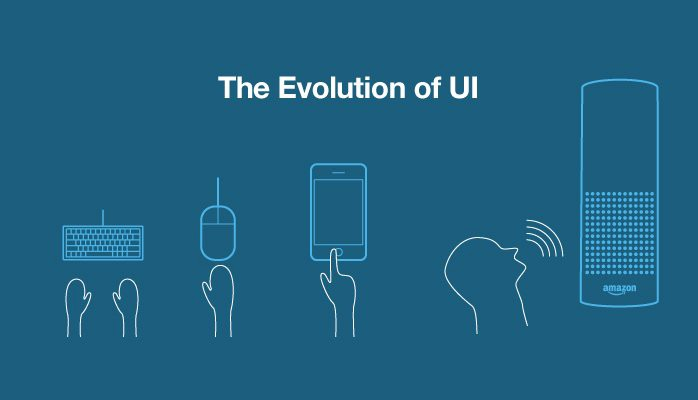
\includegraphics[width=0.9\textwidth]{bilder/evolution-ui.jpg}
    \caption{Chronologische Entwicklung von \aclp{UI} \cite{techlabs_what_2017}}
    \label{fig:evolution-ui}
\end{figure}

\subsection{Grundbegriffe}
\label{subsec:cui-grundbegriffe}

Im Folgenden werden einige Grundbegriffe, die immer wieder in Kombination mit \acp{CUI} vorkommen, erläutert.

Für den Begriff \textbf{\ac{KI}} oder \textbf{\ac{AI}} existiert eine Vielzahl von Definitionen und Interpretationen. Grundsätzlich zielt er darauf ab, einer Maschine intelligentes Verhalten anzueignen. Nach einer der ersten Definitionen für \ac{KI} von Alan M. Turing ist ein System dann intelligent, wenn es in seinen Antworten und Reaktionen nicht von einem Menschen zu unterscheiden ist \cite[S. 237]{nahrstedt_algorithmen_2012}. Der Begriff wird im Zusammenhang mit vielen anderen Forschungsbereichen verwendet, wie zum Beispiel intelligentem menschlichen Verhalten oder Entscheidungsfindung. Bezogen auf \aclp{CUI} bedeutet \acl{KI}, die Bedeutung eines Satzes herauszufinden und zuzuordnen. Dabei darf es keine Rolle spielen, wie der Nutzer seine Intention ausdrückt. \cite[S. 52]{nishith_pathak_artificial_2017}

\textbf{\ac{NLP}} beschreibt Techniken und Methoden zur maschinellen Verarbeitung natürlicher Sprache. Das Ziel ist es dabei, mit der Entwicklung neuartiger Applikationen die Interaktion zwischen Mensch und Maschine auf Basis von natürlicher Sprache zu verbessern \cite[S. 1]{deng_deep_2018}. Häufig ist in diesem Zusammenhang auch von \textbf{\ac{NLU}} die Rede, was einen Teilbereich von \ac{NLP} darstellt. Bei \ac{NLU} geht es dabei explizit darum, einen eingegebenen Text zu interpretieren und Informationen oder Intentionen daraus zu \mbox{gewinnen \cite[S. 15]{ovchinnikova_integration_2012}}.

\textbf{\ac{ML}} bezeichnet ein fundamentales Konzept zum Realisieren von \ac{KI}. Dadurch kann ein System auf Basis von Datenbeständen und Algorithmen  dazulernen, Vorhersagen treffen, Muster erkennen oder Lösungen entwickeln \cite[S. 9]{nishith_pathak_artificial_2017}. \ac{ML} ermöglicht einem System somit Entscheidungen zu treffen, ohne dass diese zuvor explizit programmiert oder vordefiniert werden \cite[S. 187]{mitrevski_developing_2018}. 

\textbf{\ac{DL}} ist eine Technik aus dem Bereich \acl{ML}. In diesem Bereich sind so genannte \acp{ANN}, quasi Modelle nach dem Vorbild von biologischen neuronalen Netzen, weit verbreitet. Mit Hilfe von \ac{DL} und der heute zur Verfügung stehenden Rechenleistung ist es nun möglich, diese sehr rechenintensiven Netzwerke schneller und zuverlässiger abzuarbeiten als herkömmliche Methoden des \aclp{ML}. Für ein möglichst intelligent und zuverlässig arbeitendes System sind dazu riesige Datenmengen, in diesem Zusammenhang oft als \textbf{Big Data} bezeichnet, nötig. \cite[S. 9]{nishith_pathak_artificial_2017}\cite[S. 9-10]{vieira_introduction_2018}

Der Begriff \textbf{\ac{DM}} bezeichnet das Systemverhalten in Abhängigkeit von Nutzeranfragen. Dabei können neben der Intention des Nutzers auch weitere Informationsquellen, wie der Gesprächsverlauf oder Ergebnisse aus Datenbankabfragen relevant sein. Die Komplexität des \ac{DM} kann dabei je nach Umfang und Eigenschaften des Systems variieren. \cite[S. 209-210]{mctear_conversational_2016}

Zwei der wichtigsten Begriffe im Bereich \ac{CUI} sind  \textbf{Intents} und \textbf{Entities}. Der \textit{Intent} gibt an, welches Vorhaben der Nutzer umsetzen will. Dazu wird die textuelle Nutzeranfrage mit Hilfe von \ac{NLU} verarbeitet und daraus der Intent extrahiert. Ist die Intention erkannt, kann eine entsprechende Aktion ausgeführt werden. Die Begriffe Intent, Intention und Vorhaben können im Verlauf dieser Arbeit als gleichwertig betrachtet werden. \textit{Entities} sind wichtige Parameter oder Schlüsselwörter in einer Nutzeranfrage. Entitäten geben wichtige Zusatzinformationen zu einem Intent an und können helfen, diesen überhaupt erst zu identifizieren. Dabei gibt es sowohl Systementitäten (z.B. Wochentag) als auch userspezifische Entitäten (z.B. Flugzeugtyp). \cite[S. 27, 44-45]{khan_build_2018}\cite[S. 12-13]{mitrevski_developing_2018} \\
Dies soll anhand eines Beispiels verdeutlicht werden. Die verwendeten Bezeichnungen für Intents, Entitäten und Parameter sind fiktiv und dienen lediglich dem besseren Verständnis. 

\begin{center}
Nutzer: \textit{„Kannst du mir einen Flug von \colorbox{SkyBlue}{Nürnberg} nach \colorbox{YellowGreen}{Berlin} buchen?“} \\
\colorbox{Peach}{[Intent erkannt: BucheFlugIntent]} \\
Chatbot: \textit{„Wann möchtest du fliegen?“}\\
Nutzer: \textit{„Am \colorbox{Rhodamine}{Freitag}“} \\
Chatbot: \textit{„Ich habe folgende Flüge gefunden.“} \\
\end{center}

Aus der ersten Frage des Nutzers kann der Intent \textbf{\textcolor{Peach}{\textit{BucheFlugIntent}}} sowie die beiden Entitäten \textbf{\textcolor{SkyBlue}{\textit{Abflughafen}}} und \textbf{\textcolor{YellowGreen}{\textit{Zielflughafen}}} ermittelt werden. Es fehlt allerdings noch die Auskunft nach dem Tag des Abflugs. Das System arbeitet dabei über eine Rückfrage und erwartet als Antwort einen Wert der Systementität \textit{Wochentag}. Gibt der Nutzer eine entsprechende Antwort (z.B. \textbf{\textcolor{Rhodamine}{\textit{Freitag}}}), hat das System alle notwendigen Daten erhalten und kann über ein entsprechendes \acl{DM} eine Antwort generieren.

\subsection{Chatbot}
\label{subsec:cui-chatbot}

Der Begriff Chatbot oder auch Chatterbot setzt sich aus den beiden Begriffen \textit{chat} \mbox{(= Gespräch)} und \textit{bot} (= Kurzform für Roboter) zusammen. In der Informatik wird ein Bot als weitgehend selbstständig laufendes Programm bezeichnet. Ein Chatbot ist somit eine Softwareanwendung zur Realisierung einer Unterhaltung zwischen Mensch und Maschine \cite[S. 232]{smolinski_innovationen_2017}. Die meisten Chatbots sind derzeit textbasiert, einige bieten allerdings auch die Möglichkeit der sprachlichen Ein- und Ausgabe. Das Ziel ist es dabei, dem Chatbot intelligentes Verhalten anzueignen und ihn dadurch für unterschiedlichste Aufgaben verwenden zu können. Um dies zu ermöglichen, werden die in \ref{subsec:cui-grundbegriffe} beschriebenen Techniken angewendet.

Einer der größten Vorteile von Chatbots im Vergleich zu herkömmlichen mobilen Applikationen ist, dass der Nutzer dem System sein Vorhaben auf natürliche Art und Weise mitteilt. Nach einer Statistik aus \cite{mcgrath_when_2018} haben immer noch 70\,\% der Menschen in reichen Ländern mangelnde oder gar keine Computerkenntnisse. \aclp{CUI} und damit auch Chatbots umgehen diese Probleme, da alle Menschen den natürlichen Gesprächsdialog kennen und verstehen. Aus Entwicklersicht ist die Verarbeitung von natürlicher Sprache jedoch schwieriger zu handhaben als beispielsweise ein \acl{UI} mit verschiedenen Buttons. Zwar funktioniert das mit modernsten \ac{NLP}-Plattformen wie \textit{Dialogflow} bereits erstaunlich gut, allerdings gibt es bei komplizierteren oder ungewöhnlicheren Formulierungen noch Probleme. Ein anderer Ansatz ist es dabei, das \acl{CUI} mit Visualisierungen zu erweitern. So kann beispielsweise eine Rückfrage seitens des Chatbots schnell und einfach durch eine Auswahl an Popup-Buttons beantwortet werden. Die Textbox am unteren Ende wird dabei zu jeder Zeit angezeigt und bietet dem Nutzer die Möglichkeit zur textbasierten Kommunikation. Mittels einer \textit{Web View} können dabei ganze \acs{HTML}-Seiten geladen und angezeigt werden. Verwendet werden sie für Aufgaben, die für ein chatbasiertes \acl{UI} nur schwer oder gar zu kompliziert umzusetzen \mbox{sind. \cite[S. 7-10]{khan_build_2018}}

Hinsichtlich der Architektur gibt es eine Reihe verschiedener Technologien, Frameworks und Plattformen um einen Chatbot zu realisieren. Im Folgenden soll daher eine Möglichkeit vorgestellt werden, die sich im Rahmen einer Recherche als plausibel und auch für die weitere Arbeit nutzbar herausgestellt hat. Das Schaubild dazu zeigt Abbildung \ref{fig:aufbau-chatbot}.

Ein \textit{User} schreibt zu Beginn der Konversation eine Nachricht über eine \textit{Messaging Platform} an das \textit{\acl{NLP}} Tool. Es gibt einige Nachrichtenplattformen, in denen Chatbots entwickelt und integriert werden können. Vorreiter in diesem Gebiet war vor allem der chinesische Messenger \textit{WeChat}, ehe in den letzten Jahren weitere Nachrichtenplattformen wie beispielsweise der \textit{Facebook Messenger} oder \textit{Slack} nachzogen \cite{rocketbots.io_china_2017}. Nach \cite{riya_study_2018} sind im Bereich \acl{NLP} derzeit die Plattformen \textit{Dialogflow, Wit.ai, Amazon lex, Luis} und \textit{IBM Watson} marktführend. Diese Plattformen kümmern sich um das \acl{NLU} und ordnen den Anfragen die Intents und Entities zu. 

Die \textit{Bot-Logic} interpretiert die Nachricht und leitet sie an das Backend, in der Abbildung \ref{fig:aufbau-chatbot} als \textit{Information Sources} dargestellt, weiter. Durch immer mehr Nutzeranfragen wird der Chatbot trainiert und kann sich dadurch stetig verbessern. Dahinter steckt das in \ref{subsec:cui-grundbegriffe} erklärte Prinzip des \textit{\acl{ML}}. Im Backend findet dann üblicherweise das \acl{DM} statt. Hier werden die Informationen verarbeitet und Entscheidungen in Form von \textit{Actions} getroffen. 

Zudem können gegebenenfalls weitere Informationsquellen, beispielsweise aus \textit{Datenbanken}, angebunden werden. Außerdem ist es möglich \textit{\acp{API}} wie zum Beispiel die \textit{Google Calendar API} zum Verwalten von Terminen in das Backend einzubinden. Gibt es Probleme mit der Dialogführung oder kommt der Chatbot an seine Grenzen, kann die Nachricht an einen echten Menschen, in der Darstellung als \textit{Human Intervention} bezeichnet, weitergeleitet werden. \cite{fourault_ultimate_2017}
\newline

\begin{figure}[htb]
    \centering
    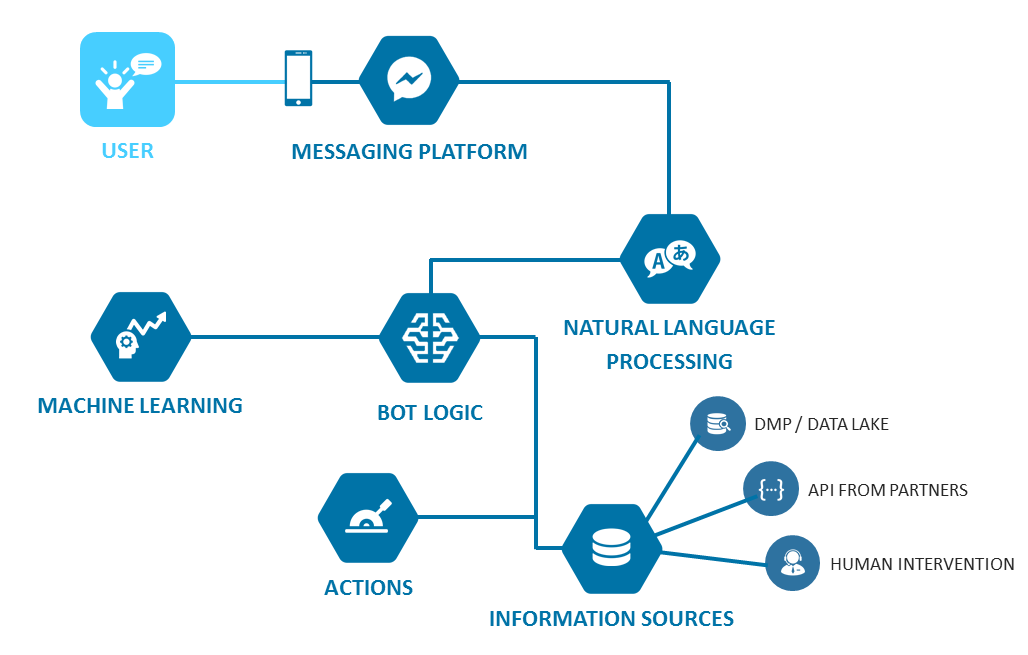
\includegraphics[width=1\textwidth]{bilder/aufbau-chatbot_v2.png}
    \caption{Aufbau eines Chatbots \cite{fourault_ultimate_2017}}
    \label{fig:aufbau-chatbot}
\end{figure}

\newpage
\section{Android Applikation}
\label{sec:basics-android-applikation}

Das Smartphone-Betriebssystem \textit{Android} hat derzeit in Deutschland einen Marktanteil von etwa 83\,\%\footnote{Stand: September 2018} \cite{statistica.com_marktanteile_2018}. Der Standard für die Entwicklung von Android Applikationen ist \textit{Java}, allerdings wird seit einiger Zeit auch \textit{Kotlin} vollständig unterstützt. Kotlin ist eine statisch typisierte Programmiersprache, die auf \ac{JVM} basiert. Einer der größten Vorteile ist dabei, dass Java und Kotlin gemeinsam innerhalb eines Projekts genutzt und sogar automatisch in die jeweils andere Sprache übersetzt werden können. Entwickelt wurde Kotlin von der Firma  \textit{JetBrains}, die auch die Entwicklungsumgebung \textit{Android Studio} zur Verfügung stellt. \cite[S. 272]{prasad_reddy_beginning_2017}

\subsection{Manifest}
\label{subsec:basics-android-manifest}

Zu Beginn jeder Android Applikation steht das \textit{Manifest}, repräsentiert durch die Datei \textit{AndroidManifest.xml}. Es nutzt \ac{XML} und dient als zentraler Punkt zur Deklaration von wichtigen Informationen über die App und ihre Komponenten. Hier werden unter anderem Aktivitäten, Services und Berechtigungen eingetragen \cite[S. 41]{allen_beginning_2015}. Im Folgenden ist eine beispielhafte Manifest Datei dargestellt, welche einen grundlegenden Eindruck vom Aufbau vermitteln soll.
\newline

\begin{lstlisting}[caption={Beispielhafte AndroidManifest.xml Datei}, captionpos=b, label={lst:manifest-xml}, language=XML]
<?xml version="1.0" encoding="utf-8"?>
<manifest xmlns:android="http://schemas.android.com/apk/res/android"
    package="com.example.michaelwagner.beispiel">
    
    <uses-permission android:name="android.permission.INTERNET"/>
    
    <application
        android:allowBackup="true"
        android:icon="@mipmap/ic_launcher"
        android:label="@string/app_name"
        android:roundIcon="@mipmap/ic_launcher_round"
        android:supportsRtl="true"
        android:theme="@style/AppTheme">
        <activity android:name=".Activities.MainActivity">
            <intent-filter>
                <action android:name="android.intent.action.MAIN" />
                <category android:name="android.intent.category.LAUNCHER" />
            </intent-filter>
        </activity>
        <activity android:name=".Activities.SecondActivity"></activity>
    </application>
</manifest>
\end{lstlisting}

Der Name hinter dem Tag \textit{package} dient der Identifikation der App auf dem Smartphone oder auch im \textit{Google Play Store}. Durch die Angabe von \textit{uses-permission} können diverse Berechtigungen, wie hier etwa \textit{INTERNET} zur Herstellung von Internetverbindungen, erteilt werden. Einige häufig verwendete Permissions sind \textit{CAMERA} für Kamerazugriff, \textit{ACCESS\_FINE\_LOCATION} für den genauen Standort und \mbox{\textit{RECORD\_AUDIO}} zur Sprachaufnahme via Mikrofon. Das Element \textit{application} definiert das Anfangsverhalten der App. Die Attribute für \textit{icon}, \textit{label} oder \textit{theme} definieren Basisinformationen wie das Icon oder den Namen für die App. Außerdem muss jede \textit{activity} dort eingetragen sein. Dabei muss auch eine \textit{Launcher Activity} deklariert werden, die der Nutzer als Erstes beim Start der App sieht.. \cite[S. 42-43]{allen_beginning_2015}\cite{android_developers_app_2018}

\subsection{Layout}
\label{subsec:basics-android-layout}

Wie schon beim Manifest wird auch für das Layout einer Android App die erweiterbare Auszeichnungssprache \ac{XML} genutzt. Das Layout definiert den Aufbau des \aclp{UI}. Unterschieden werden dabei \textit{View}- und \textit{ViewGroup}-Objekte. Eine ViewGroup ist eine Art unsichtbarer Container, der die Struktur für weitere Elemente vorgibt. Jede Layout-Datei besitzt dabei genau eine übergeordnete ViewGroup, die für das gesamte \ac{UI} gilt. Nach \cite[S. 79-80]{allen_beginning_2015} sind die am häufigsten verwendeten Layout-\mbox{Container}:
\begin{itemize}
\item\textbf{RelativeLayout} - Verschiedene Regeln zur relativen Anordnung der Elemente unter-, über- oder nebeneinander 
\item\textbf{LinearLayout} - Alle Elemente werden in einer Richtung, horizontal oder vertikal, angeordnet
\item\textbf{ConstraintLayout} - Keine verschachtelten ViewGroups, alle Elemente werden relativ angeordnet, über so genannte Constraints (Regeln)
\end{itemize}

Eine View ist die Basisklasse eines \textit{Widgets}, wie \textit{Button} oder \textit{TextView}. Widgets werden genutzt, um ein interaktives \acl{UI} zu erstellen \cite[S. 137]{jackson_learn_2013}. Die Views und ViewGroups unterstützen verschiedene Attribute. Dabei gibt es sowohl Attribute für alle Elemente als auch spezifische Attribute, die nur bestimmte Elemente implementieren können. Generell sollten bei der Angabe von Höhe, Breite oder Schriftgröße konstante Werte vermieden werden. Besser ist die Angabe von relativen Maßen wie \textit{\ac{dp}}, \textit{wrap\_content} oder \textit{match\_parent}, weil dadurch sichergestellt wird, dass die App auch auf unterschiedlichen Bildschirmgrößen korrekt dargestellt wird. Tabelle \ref{tab:attributes-layout-elements} zeigt eine kleine Auswahl an Attributen inklusive Beispielwert und Bedeutung. \cite{android_developers_layouts_2018}
\newline
\def\arraystretch{1.5}
\begin{table}[ht!]
    \centering
    \begin{tabular}{| C{3.5cm} | C{2.5cm} | C{7cm} | } 
    \hline \textbf{Attribut} & \textbf{Beispielwert} & \textbf{Bedeutung} \\ [0.5ex] 
    \hline android:id & @+id/my\_button & Eindeutiger Identifier des Elements \\
    \hline android:layout\_width & wrap\_content  & Breite des Elements an Inhalt anpassen \\
    \hline android:layout\_height & match\_parent & Höhe des Elements wie übergeordnetes Element  \\
    \hline android:text & Das ist ein Text & Textinhalt des Elements \\
    \hline android:textSize & 12dp & Schriftgröße des Elements \\
    \hline android:background & \#f9aa20 & Hintergrundfarbe des Elements \\
    \hline
    \end{tabular}
    \caption{Attribute von Layout-Elementen}
    \label{tab:attributes-layout-elements}
\end{table}

\subsection{Activity}
\label{subsec:basics-android-activity}

Eine Aktivität (engl. \textit{Activity}) repräsentiert einen Bildschirm, mit dem der Nutzer interagieren kann. Die Aktivität selbst stellt dabei in der Regel keine Benutzeroberfläche bereit, sondern ist mit einem entsprechen \ac{XML}-Layout verknüpft. Ein äußerst wichtiges Prinzip im Zusammenhang mit Aktivitäten ist der Lebenszyklus. Dabei werden Aktivitäten via \textit{Callback}-Methoden über Zustandsänderungen informiert. Jede dieser Methoden kann überschrieben werden. \cite[S. 187-188]{gerber_learn_2015}\cite{programmieren_lernen_programmier_2018} 

\clearpage
Die verschiedenen Zustände und dazugehörigen Methoden werden im Folgenden anhand von Abbildung \ref{fig:android-lebenszyklus-acitvity} ausführlich erläutert. 

\begin{itemize}
\item\textbf{onCreate()}: Wird beim erstmaligen Erzeugen der Aktivität aufgerufen. Hier sollten Initialisierungen vorgenommen, Views erzeugt oder Daten geladen werden. Anschließend wird \textit{onStart()} aufgerufen.

\item\textbf{onRestart()}: Die Aktivität muss zuvor gestoppt worden sein. Der Aufruf erfolgt, wenn User zu der Activity zurück navigiert. Der Methode folgt immer \textit{onStart()}.

\item\textbf{onStart()}: Wird aufgerufen, kurz bevor die Aktiviät auf dem Bildschirm sichtbar wird. Anschließend wird \textit{onResume()} aufgerufen. 

\item\textbf{onResume()}: Diese Methode wird ausgeführt, wenn die Aktivität bereit für Benutzereingaben ist. Nach Beendigung dieser Methode wird die Aktivität ausgeführt.

\item\textbf{onPause()}: Wird kurz vor dem Start einer anderen Aktivität aufgerufen. Geänderte Daten oder Zustände sollten an dieser Stelle gespeichert werden. Anschließend wird \textit{onResume()} aufgerufen, wenn die Activity wieder in den Vordergrund rückt oder \textit{onStop()}, wenn sie verdeckt wird. 

\item\textbf{onStop()}: Wird aufgerufen, wenn die Aktivität nicht mehr sichtbar ist. Nach dieser Methode kann das Android-System den App-Prozess aufgrund von Speicherplatzmangel direkt beenden. Anschließend folgt die \textit{onRestart()} Methode, wenn die Activity wieder fortgesetzt wird oder die \textit{onDestroy()} Methode, wenn die Activity endgültig zerstört wird.

\item\textbf{onDestroy()}: Aufruf kurz vor dem Zerstören der Aktivität. Erfolgen kann dies planmäßig innerhalb der Applikation oder durch das Android-System. Nachdem dies der letzte Aufruf ist, folgt keine weitere Methode.

\end{itemize}

\begin{figure}[htb]
    \centering
    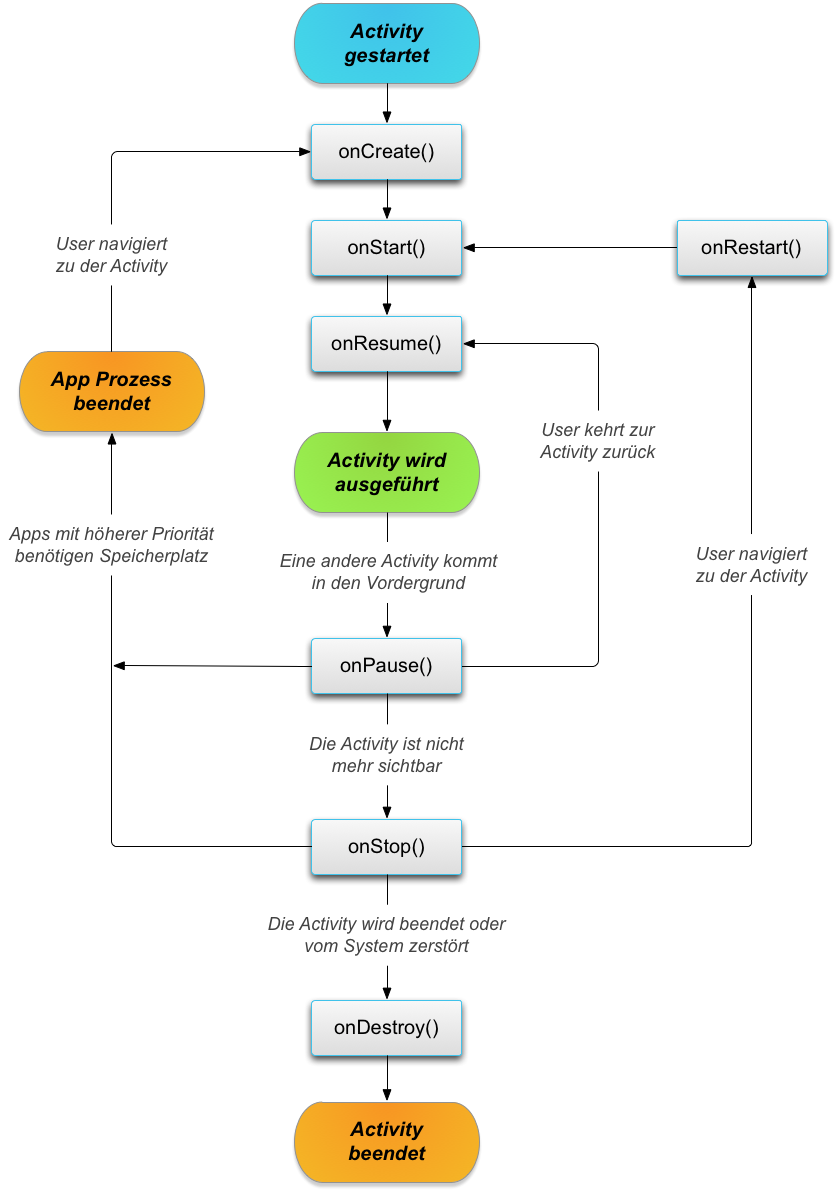
\includegraphics[width=1\textwidth]{bilder/android_activity_lifecycle.png}
    \caption{Lebenszyklus einer Aktivität \cite{programmieren_lernen_programmier_2018}}
    \label{fig:android-lebenszyklus-acitvity}
\end{figure}


\chapter{Konzeption}
\label{cha:konzeption}

In diesem Kapitel werden die Anforderungen an den Chatbot und ein Konzept für die Implementierung erarbeitet.  Dafür werden Ansichten und Methoden aus dem Bereich \textit{Usability Engineering} verwendet. Usability wird auch als Gebrauchstauglichkeit bezeichnet und definiert sich wie folgt: 

\begin{quote}
    Das Ausmaß, in dem ein Produkt durch bestimmte Benutzer in einem bestimmten Nutzungskontext dazu genutzt werden kann, bestimmte Ziele effektiv, effizient und zufriedenstellend zu erreichen \cite[S. 11]{richter_usability_2016}.
\end{quote}

Der \textit{Nutzungskontext} umfasst dabei die Benutzer, deren Aufgaben, soziale und physische Umgebung sowie die aufgewendeten Ressourcen. Die \textit{Effektivität} misst dabei die Vollständigkeit und Genauigkeit der Zielerreichung. Das Kriterium \textit{Effizienz} bezeichnet den Aufwand und die Ressourcen zur Zielerreichung. Die \textit{Zufriedenstellung} gibt Auskunft über die Freiheit von Beeinträchtigungen und positive Einstellung des Benutzers gegenüber dem System. 

Die Definition von Usability impliziert dabei jedoch immer eine sehr funktionsbezogene Betrachtungsweise. Um auch Aspekte wie Emotionen, Ästhetik und Wahrnehmungen zu betrachten, kann das Konzept der \textit{\ac{UX}} angewendet werden. Die \acl{UX} erweitert die Usability und definiert sich wie folgt:

\begin{quote}
   Wahrnehmungen und Reaktionen einer Person, die aus der tatsächlichen und/oder der erwarteten Benutzung eines Produktes, eines Systems oder einer Dienstleistung resultieren \cite[S. 14]{gast_user_2018}.
\end{quote}

\ac{UX} umfasst demnach auch Effekte auf den Nutzer, die ein System bereits vor oder auch nach seiner Verwendung hat. Diese Empfindungen haben wiederum Einfluss auf den nachfolgenden Aspekt (\textit{„Nach der Nutzung ist vor der Nutzung“}).
Die Usability bleibt dennoch ein wichtiger Faktor und Teil der \acl{UX}. Aufgrund der umfassenderen Betrachtungsweise wird der Begriff \ac{UX} immer öfter auch anstelle der Bezeichnung \textit{Usability} verwendet. Abbildung \ref{fig:usability-user-experience} erläutert die beiden Begriffe anhand einer grafischen Darstellung.
\newline

\begin{figure}[htb]
    \centering
    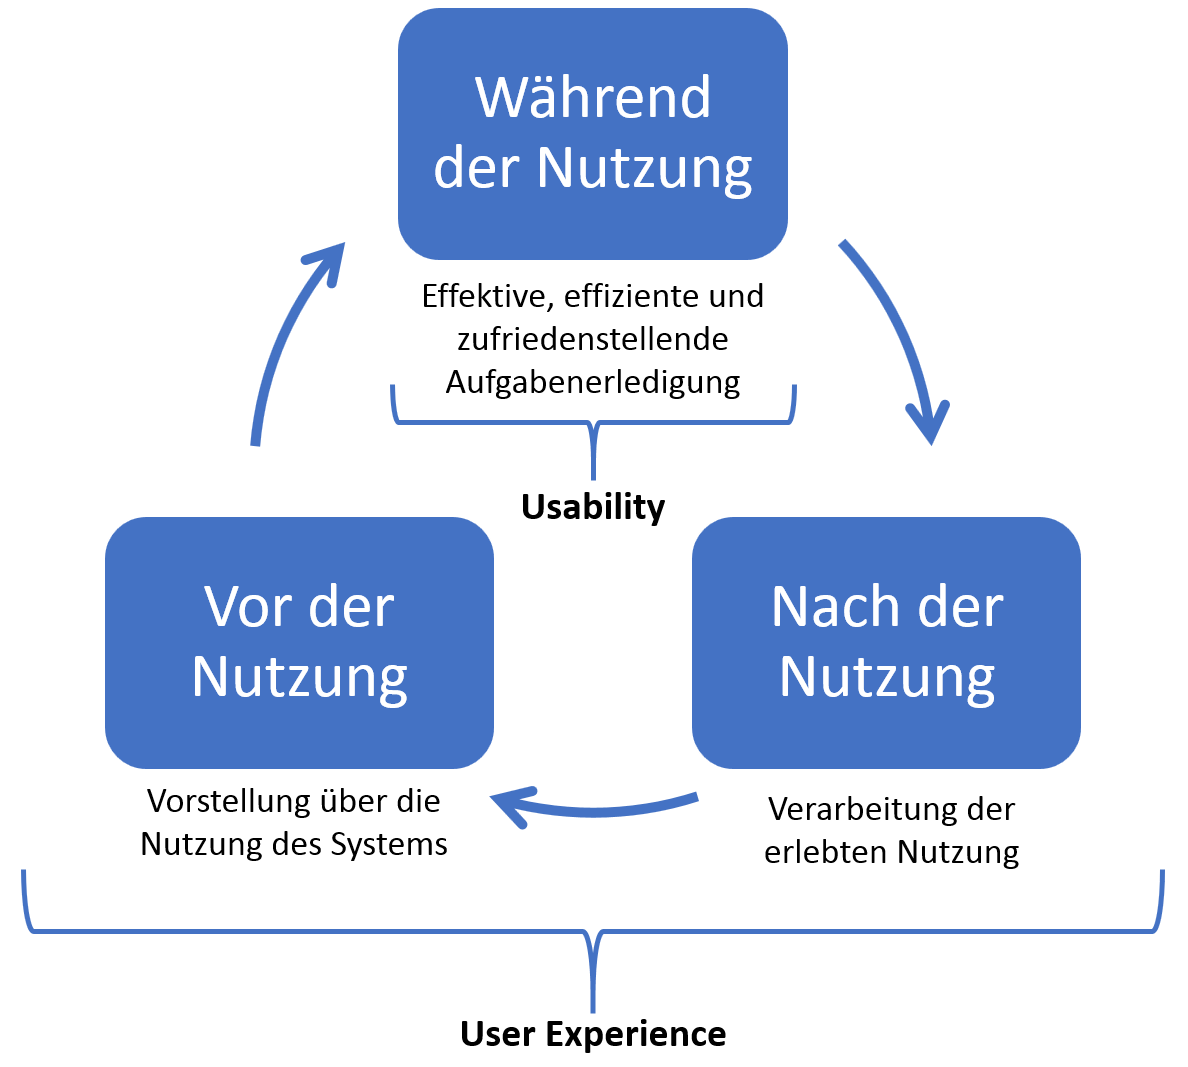
\includegraphics[width=0.8\textwidth]{bilder/usability-user-experience_v2.png}
    \caption{Usability und \acl{UX}}
    \label{fig:usability-user-experience}
\end{figure}

Sowohl Usability als auch User Experience stellen einen wichtigen Faktor in der Softwareentwicklung dar. Gerade im Bereich der \aclp{CUI} ist die Anwendung dieser Konzepte und Methodiken äußerst wichtig. Nachdem der Benutzer beim \ac{CUI} auf natürliche Art und Weise mit dem System interagiert, müssen Formulierungen und Ausdrucksweisen fehlerfrei erkannt und interpretiert werden. Zudem müssen auch eventuelle Rückfragen, Statusmeldungen oder Antworten korrekt und ohne Spielraum für Missinterpretationen formuliert werden. 

Ein weiterer wichtiger Aspekt in diesem Zusammenhang ist das \textit{\ac{UCD}}, im Deutschen oft als \textit{menschzentrierter Gestaltungsprozess} übersetzt. Diese nutzerzentrierte Gestaltung zielt darauf ab, interaktive Produkte so zu gestalten, dass sie über eine hohe Gebrauchstauglichkeit verfügen. Der Begriff beschreibt Gestaltungsprozesse, die den zukünftigen Benutzer mit seinen Aufgaben, Zielen und Eigenschaften ins Zentrum des Entwicklungsprozesses stellen. Dabei spielt die frühe Fokussierung auf den Nutzer und dessen Anforderungen eine entscheidende Rolle. Der Prozess sieht außerdem Iterationen vor, sobald Evaluierungsergebnisse Bedarf dafür aufzeigen. \cite[S. 67-68]{tryfonas_human_2016} 

Diese Vorgehensweise hat sich in den letzten Jahren bei der Entwicklung von Mobile- und Webapplikationen bewährt. Die grundlegenden Nutzeranforderungen ändern sich nicht durch einen Wechsel des Interfaces von \ac{GUI} zu \ac{CUI}. Es muss jedoch verstanden werden, welche Methoden und Techniken in diesem Zusammenhang sinnvoll sind und verwendet werden sollten. Werden diese Aspekte bei der Entwicklung eines Chatbots angewendet, so können auch hier wertvolle Daten gesammelt werden, woraus dann hochwertige \aclp{UI} entstehen. \cite{chandra_how_2018} 

Die Inhalte des \textit{\acl{UCD}} sind in der \textit{ISO 9241-210} festgehalten und können anhand von Abbildung \ref{fig:user-centered-design} grafisch dargestellt werden.
\newline

\begin{figure}[htb]
    \centering
    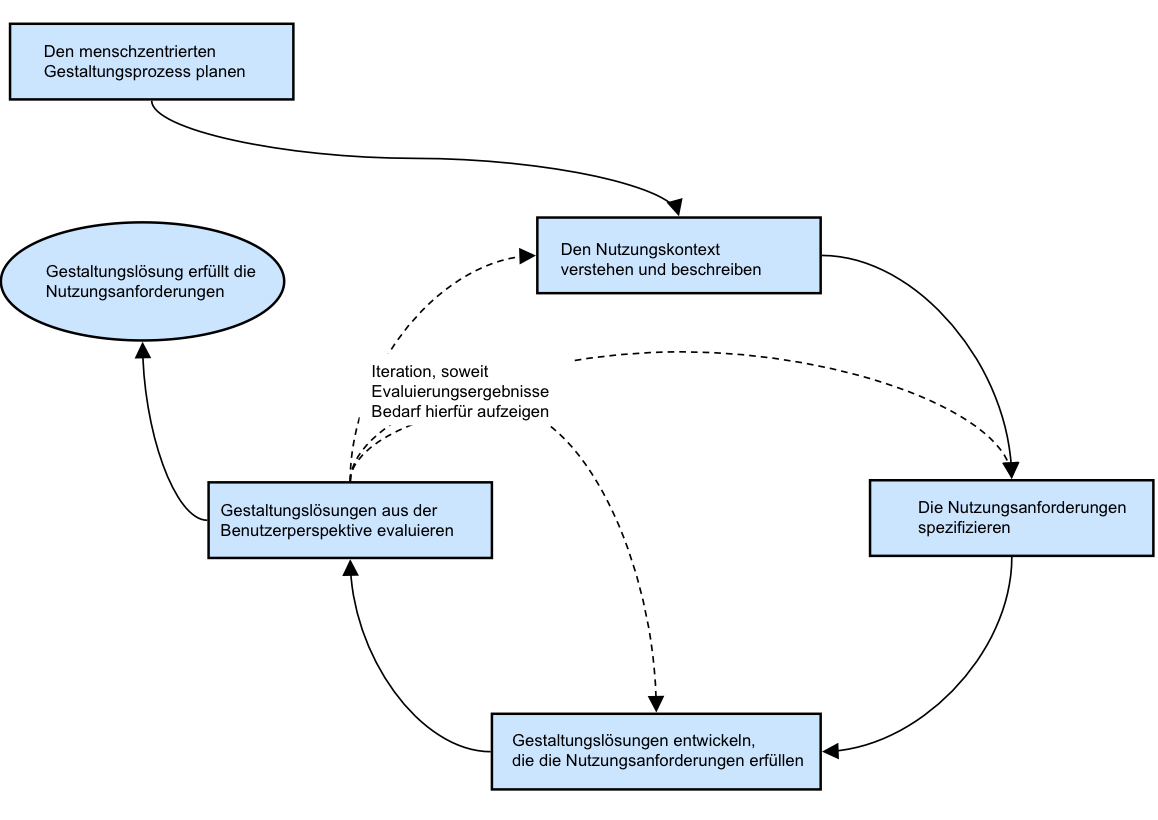
\includegraphics[width=1.0\textwidth]{bilder/user-centered-design.png}
    \caption{\acl{UCD} - Menschzentrierter Gestaltungsprozess \cite{geis_neue_2010}}
    \label{fig:user-centered-design}
\end{figure}

Um all diese Ziele zu erreichen, werden zunächst Überlegungen hinsichtlich des Requirements Engineering angestellt. Dazu können verschiedene Techniken aus dem Bereich des Usability- und Requirements Engineering eingesetzt werden. Mit Hilfe einer prototypischen Umsetzung können diese Überlegungen anschließend überprüft und evaluiert werden.

\section{Requirements Engineering}
\label{sec:requirements-engineering}

Requirements Engineering befasst sich damit, die Bedürfnisse der Benutzer, Auftraggeber
und weiterer Interessengruppen, im Allgemeinen auch als Stakeholder bezeichnet, hinreichend aufzuarbeiten \cite[S. 23]{richter_usability_2016}. Darauf basierend können dann Rückschlüsse auf die Rahmenbedingungen, Qualitätsanforderungen sowie vorgesehene Funktionen und Systemverhalten geschlossen werden. 

\subsection{Fragebogen}
\label{subsec:fragebogen}

Um einen groben Überblick über die Thematik zu erhalten, sollen zunächst das Verhalten und die Präferenzen bei der Raumbuchung im Office der \adorsys\ erfasst werden. Um eine mögliche Voreingenommenheit gegenüber Chatbots zu vermeiden, wird der Hintergrund und das explizite Thema der Masterarbeit in diesem Zusammenhang nicht erwähnt. Die Zielgruppe sind dabei alle Mitarbeiter der \adorsys\ unabhängig davon, wie oft diese in der Regel einen Raum buchen. 

Um möglichst alle relevanten Informationen einzufangen, soll dazu ein Online-Frage\-bogen erstellt werden. Mit dessen Hilfe lassen sich quantitative Daten sammeln und direkt elektronisch auswerten. Zur Erstellung und Durchführung des Fragebogens werden im Folgenden die Anwendungen \textit{Survey Monkey}, \textit{Typeform} und \textit{Google Forms} genauer betrachtet. Dazu wird, wenn es unterschiedliche Varianten gibt, jeweils die kostenlose Basisvariante der Anwendungen untersucht. Die kostenlosen Varianten der Anwendungen werden verwendet, um möglichst keine Mehrkosten zu generieren sowie den Aufwand und die damit verbundenen Verzögerungen minimal zu halten. Die Anforderungen resultieren aus den Rahmenbedingungen des zuvor erstellten Fragebogens. So besteht dieser aus 18 Fragen, bei denen es sich hauptsächlich um Basis-Fragetypen wie Multiple-Choice, Textfelder oder linearen Skalen handelt. Relevant ist dabei auch die Anonymisierung der Daten, um möglichst ehrliche und ungefilterte Antworten zu erhalten. Das Unterbinden einer Mehrfachteilnahme ist ebenso wünschenswert. 

Der vollständige Fragebogen ist aus Gründen der besseren Lesbarkeit im Anhang \ref{sec:anhang-fragebogen} zu finden. 
Tabelle \ref{tab:umfrage-toolauswahl} zeigt eine Übersicht der Anforderungen und betrachteten Anwendungen. Erfüllte Anforderungen sind dabei mit einem \textit{grünen Haken}, nicht erfüllte mit einem \textit{roten Kreuz} versehen. Ein \textit{gelbes Warndreieck} sagt aus, dass die Anforderung nur unter einer bestimmten Bedingung erfüllt werden kann. Die Inhalte der Tabelle stützen sich auf die Informationen aus \cite{surveymonkey_surveymonkey_2018}, \cite{typeform_plans_2018} und \cite{google_forms_google_2018}.
\newline

\begin{table}[!htb]
\centering
 \begin{tabular}{ | m{5cm} || C{2cm}| C{2cm} | C{2cm} |} 
 \hline
 Anforderungen & Survey Monkey & Typeform & Google Forms 
 \\
 \hhline{=::===}
 18 Fragen & \xmark & \xmark & \cmark\\ 
 \hline Basis-Fragetypen & \cmark & \cmark & \cmark \\
 \hline Anonymisierung & \cmark & \cmark & \cmark\\ 
 \hline Mehrfachteilnahme unterbinden & \cmark & \danger & \cmark\\ 
 \hline
\end{tabular}
\caption{Auswahl einer Anwendung für den Fragebogen}
\label{tab:umfrage-toolauswahl}
\end{table}

Die beiden Anwendungen Survey Monkey und Typeform ermöglichen in der Basisvariante nur maximal zehn Fragen. Bei Google Forms gibt es eine solche Beschränkung dagegen nicht. Die für den Fragebogen relevanten Basis-Fragetypen wie Multiple-Choice, Textfelder oder lineare Skalen unterstützen dagegen alle Anwendungen. Gleiches gilt für die Möglichkeit, die erfassten Daten zu anonymisieren. Die Unterbindung einer Mehrfachteilnahme ist mit Typeform nur über Umwege möglich, wird von Survey Monkey und Google Forms dagegen standardmäßig unterstützt. Aufgrund der erläuterten Kriterien fällt die Wahl der Anwendung auf Google Forms. Die Anwendung unterstützt alle Anforderungen und kann ohne zusätzliche Kosten genutzt werden. 

Im Folgenden werden einige markante Ergebnisse aus dem Fragebogen herausgegriffen und genauer betrachtet. Die Fragen sind dabei oft nach Schlagwörtern wie \textit{gewöhnlich} oder \textit{in der Regel} gestellt und müssen daher mit Vorsicht betrachtet werden, um keine falschen Rückschlüsse auf die Ergebnisse zu ziehen. 

Knapp die Hälfte der Befragten buchen täglich oder alle zwei bis drei Tage einen Raum. Dabei ist erwähnenswert, dass sich der Fragebogen auf die Raumbuchung im Office der \adorsys\ bezieht und einige der Befragten durch Ihre Tätigkeit bei Kunden und in Projekten oft außerhalb des Büros arbeiten. Daraus lässt sich schließen, dass das Buchen von Räumen bei vielen Mitarbeitern ein fester Bestandteil des Arbeitsalltags ist. 

Über 60\,\% der Buchungen werden dabei mindestens einen Tag im Voraus getätigt, mit knapp 2\,\% gibt es vergleichsweise wenige Buchungen über Wochen oder Monate im Voraus. Erklären lässt sich dies dadurch, dass weit im Voraus geplante Termine oft einen Workshop- oder Schulungs-Charakter haben, über mehrere Stunden gehen und eine größere Anzahl an Teilnehmern besitzen. Diese müssen entsprechend frühzeitig geplant werden, kommen aber vergleichsweise selten vor. 

Erwähnenswert ist außerdem das Ergebnis auf die Frage nach der gewöhnlichen Besprechungsdauer. Über 90\,\% der Teilnehmer geben an, dass ihre Besprechungen in der Regel weniger als zwei Stunden dauern. Dies ist möglicherweise auf die Vielzahl an relativ häufigen und gleichermaßen kürzeren Termine wie beispielsweise Code-Reviews, Team-Meetings aber auch Vorstellungs- oder Mitarbeitergesprächen zurückzuführen. 

Einige Fragen beziehen sich auf das \textit{E-Paper Display} am Eingang der Besprechungsräume, welches den aktuellen Status des Raumes sowie das nächste anstehende Meeting anzeigt. Außerdem bietet es durch Bedienung die Möglichkeit, den Belegungsplan des Raumes einzusehen und den Raum direkt oder zu einem späteren Zeitpunkt zu reservieren. Nach den Ergebnissen aus dem Fragebogen nutzen etwa zwei Drittel das E-Paper Display, wenn sie sofort einen Raum benötigen. Um einen Raum zu einem späteren Zeitpunkt zu verwenden, nutzen es dagegen nur knapp 8\,\%. Als Grund hierfür könnte die Bedienung eine Rolle spielen. Wenn sofort ein freier Raum benötigt wird, zeigt das Display den Status des Raumes an und bietet die Möglichkeit, den Raum über einen Klick zu reservieren. Für eine Reservierung zu einem späteren Zeitpunkt ist eine aufwendigere Bedienung des E-Paper Displays nötig. 

Mehr als die Hälfte der Teilnehmer finden eine Bestätigung der Raumbuchung sinnvoll. Als häufigste Gründe dafür werden das Vermeiden von Leerbuchungen und eine gesteigerte Konsistenz von Buchung zum tatsächlichen Status genannt. Auf der Gegenseite stehen Bedenken in Form von Vergessen der Bestätigung sowie Mehrarbeit und zusätzlicher Aufwand bei der Buchung. 

Auf die Frage nach bevorzugten Räumen bei der Buchung gibt es relativ eindeutige Ergebnisse. Knapp 60\,\% der Befragten nannten in diesem Zusammenhang die Räume R1, R2 und R4. Häufig genannte Gründe hierfür sind die angenehme Raumgröße für bis zu acht Personen und die Helligkeit des Raumes durch die großen Fenster (Tageslicht). Den Raum R3 bevorzugen nur etwa 28\,\% der Teilnehmer und führen dies meist auf die Nutzung des Videokonferenzsystems zurück. Da dieser Raum keine Fenster für direktes Tageslicht hat, ist er auch weniger beliebt. Die Räume R3 und R4 sind durch ein Milchglas bzw. einen Vorhang zusätzlich diskreter, was für die Befragten bei gewissen Terminen relevant ist. Außerdem stimmten etwa 12\,\% für den Raum R6 und begründeten dies mit der großen Anzahl an Teilnehmern. 

Es besteht außerdem die Möglichkeit, Besprechungsräume über einen \textit{Slackbot} zu reservieren. Ein Slackbot ist sozusagen ein Chatbot innerhalb der Nachrichtenplattform Slack. Dieser kann über eine \ac{API} relativ einfach eingerichtet werden. Damit ist es möglich, Räume kommandobasiert abzufragen oder zu reservieren. Nach den Ergebnissen des Fragebogens wird dieser Slackbot allerdings bisher kaum bis gar nicht genutzt. Dies ist möglicherweise auf die Bedienung zurückzuführen. Auf die Frage, wie die Befragten am liebsten ihre Raumbuchung durchführen würden, antworteten aber immerhin 6,5\,\% mit der Antwort: \textit{Slackbot}. Daraus lässt sich schließen, dass der Wunsch nach der Durchführung einer Raumbuchung über ein \acl{CUI} bei einigen Nutzern vorhanden ist, bisher aber noch nicht zufriedenstellend erfüllt \mbox{wurde}.

\subsection{Interviews}
\label{subsec:interviews}

Durch den Fragebogen ist es möglich, einen allgemeinen Einblick in das Verhalten und die Präferenzen bei der Raumbuchung zu erhalten. Diese Methode liefert allerdings hauptsächlich quantitative Daten. Um einen tieferen Einblick in das Nutzungsverhalten zu erlangen, sollen nun qualitative Daten gesammelt werden. Diese Daten können im Rahmen eines Interviews erhoben werden. Diese Methode bietet den Vorteil, direkt auf die Antworten des Interviewten eingehen zu können und mögliche Unklarheiten sofort zu beseitigen. Zudem liefert ein Interview durch die direkte Kommunikation sehr komplexe und detaillierte Daten. Damit ist gemeint, dass zusätzlich zu den verbalen Aussagen auch die Mimik und Gestik des Befragten wertvolle Hinweise liefern kann. 

Bei der Auswahl der Probanden wird Wert darauf gelegt, unterschiedlichste Charaktere und Rollen zu interviewen. Diese sollen sich sowohl im Tätigkeitsfeld, als auch in ihren technischen Fähigkeiten oder Präferenzen unterscheiden. Die Haupttätigkeitsfelder der vier Interviewten sind in Tabelle \ref{tab:interviewte-taetigkeitsfeld} dargestellt.
\newline

\begin{table}[H]
\centering
 \begin{tabular}{ | C{2cm} || C{5cm} || C{2cm} |} 
 \hline
 Interviewter & Haupttäigkeitsfeld & Kürzel \\
 \hhline{=::==}
 \hline I1 & Development & D \\ 
 \hline I2 & Coaching & C\\ 
 \hline I3 & Human Resources & HR \\ 
 \hline I4 & Vertrieb & V \\ 
 \hline
\end{tabular}
\caption{Haupttätigkeitsfelder der Interviewten}
\label{tab:interviewte-taetigkeitsfeld}
\end{table}

Im Verlauf des Interviews wird dabei auf verschiedene Zusammenhänge und Hintergründe im Kontext einer Raumbuchung eingegangen. Die Kernpunkte und Überbegriffe des Interviewleitfadens sind nachfolgend aufgelistet. 

\begin{itemize}
    \item Vorgehen/Ablauf bei der Raumbuchung
    \item Fragen zum E-Paper Display 
    \item Fragen zum Zeitmanagement
    \item Ergänzende Fragen
\end{itemize}

Ein vollständiger Interviewleitfaden mit allen Fragen ist in Anhang \ref{sec:anhang-interviewleitfaden} zu finden. Um sicherzustellen, dass keine Informationen verloren gehen, wird das Interview mit einem Aufnahmegerät aufgezeichnet. Der Interviewer kann während des Interviews Notizen anfertigen und eine ausführliche schriftliche Auswertung nachträglich durch- führen. Eine entsprechende Einverständniserklärung wird jedem Teilnehmer vor Beginn des Interviews zur Unterschrift vorgelegt. Diese ist im Anhang \ref{sec:anhang-einverstaendnis-interview} zu finden. 

In Bezug auf die Durchführung eines Interviews gibt es einige wichtige Verhaltensregeln. So ist es zunächst wichtig, dem Teilnehmer einen neutralen und vertrauenswürdigen Eindruck zu vermitteln. Dazu können so genannte \textit{Warming-Up Fragen} als Eisbrecher genutzt werden. Die Fragen im Verlauf des Interviews sollten neutral formuliert werden, sodass sie den Befragten nicht in eine Richtung lenken. Um optimale Ergebnisse zu erzielen, kann das \textit{Meister-Schüler-Modell} angewendet werden. Der Interviewte ist dabei der Meister, der Interviewer der Schüler. Alles, was der Meister sagt, ist richtig. Der Interviewer passt sich also dem Interviewten an, widerspricht und verbessert ihn nicht. Der Teilnehmer kann keine falschen Antworten geben. Ziel des Interviews ist es, die Gedanken und Meinungen des Nutzers zu erfassen und zu \mbox{verstehen}. 

Nachfolgend sollen einige Auffälligkeiten, Übereinstimmungen oder auch Diskrepanzen im Rahmen der vier Interviews beschrieben werden. Eine ausführliche, schriftliche Auswertung ist im Anhang \ref{sec:anhang-interview-auswertung} zu finden. 

Auffällige Übereinstimmungen gibt es im Raumbuchungsverhalten, sowohl um einen Raum jetzt sofort, als auch zu einem späteren Zeitpunkt zu buchen. Wie bereits im Fragebogen erkennbar war, werden die E-Paper Displays nur genutzt um einen Raum für jetzt sofort zu buchen. Dieses Vorgehen ist bei allen Interviewten nahezu identisch. Es wird zunächst physikalisch in den Raum und am E-Paper nachgeschaut, ob der Raum frei ist und dieser wird anschließend direkt per Knopfdruck gebucht. Wird ein Raum zu einem bestimmten Zeitpunkt in der Zukunft benötigt, bevorzugen die Interviewten eine Raumbuchung am Rechner über das \textit{Web Interface} vom Google-Kalender. Folgende Stärken und Schwächen wurden in diesem Zusammenhang erwähnt. In den nachfolgenden Klammern steht jeweils, wie oft der Aspekt erwähnt wurde.

\begin{itemize}
    \item[+] Freie Zeiten von Räumen und Personen nebeneinander darstellen (3)
    \item[+] Überblick und Übersichtlichkeit (3)
    \item[+] Längere Termine oder Serientermine (1)
    \item[+] Feedback falls Raum nicht frei (1)
    \item[+] Andere Leute können Termin bearbeiten (1)
    \item[+] Möglichkeit zum Einplanen von Pufferzeiten (1)
    \item[+] Überall verfügbar, sowohl Office als auch privater Rechner (1)
    \item[-] Anfrage zum Verschieben bzw. Verlegen von anderen Terminen (2)
    \item[-] Keine genaue Information bei Konflikt in wiederkehrendem Termin (1)
    \item[-] Räume fälschlicherweise als verfügbar angezeigt (1)
    \item[-] Raumnamen irritierend (1)
    \item[-] Hangout-Link standardmäßig im Termin (1)
    \item[-] Kürzel der Teilnehmer unpersönlich (1)
    \item[-] Teams bzw. Gruppen definieren (1)
\end{itemize}

In Bezug auf die Verwendung des Slackbots äußerte I1, dass bei der Verwendung unklar ist was geschrieben werden muss, um einen Raum zu buchen. Außerdem sind die Antworten bzw. das Feedback des Slackbots nicht hilfreich. Dies deckt sich mit der Interpretation der Ergebnisse des Fragebogens aus \ref{subsec:fragebogen}. 

Auch die Frage nach der Bestätigung der Raumbuchung spiegelt in etwa die Eindrücke aus dem Fragebogen wider. Die prinzipiellen Vorteile dieser Idee, wie die Vermeidung von Leerbuchungen oder die bessere Konsistenz des Raumstatus, erscheinen allen Interviewten als sinnvoll. Allerdings gibt es auch hier Bedenken hinsichtlich der Umsetzung und Art der Bestätigung. Außerdem sind dabei unterschiedliche Betrachtungsweisen aufgefallen. Der einen Ansicht nach ist es besser, wenn Besprechungsräume einen freien Raumstatus anzeigen, aber dennoch belegt sind. Der anderen Ansicht nach ist es besser, wenn die Räume im Zweifel belegt anzeigen und dann doch frei sind. Dies soll durch ein Zitat von I2 verdeutlicht werden: \textit{„Ich find‘s blöder wenn belegt ist und frei drin steht als wenn‘s andersrum der Fall ist"}

 Der Wunsch nach Diskretion tauchte mehrfach im Rahmen der Interviews auf. So äußerte I3 den Wunsch nach einer Art \textit{Privatisierung} des E-Paper Displays bei gewissen Terminen, wie Mitarbeiter- oder Vorstellungsgesprächen. Es soll von außen nicht erkennbar sein, welchen Titel der Termin hat. Nachdem das E-Paper allerdings nur den Titel aus dem Kalender anzeigt, ist dies eher als Problem auf den Google-Kalender zurückzuführen. Weiterhin spielte in diesem Zusammenhang die Auswahl des Besprechungsraums eine Rolle. Wirklich diskret, begünstigt durch Milchglas bzw. einen Vorhang, sind nur die beiden Besprechungsräume R3 und R4. Diesen Aspekt äußerte I3 ebenfalls bei der Frage nach bevorzugten Räumen. 

Generell decken sich die Aussagen bezüglich der bevorzugten Räume mit den Ergebnissen des Fragebogens. Die Räume R1, R2 und R4 sind aufgrund der Helligkeit durch Tageslicht und ihre angenehme Größe sehr beliebt. Der Raum R4 hat durch seine Hochstühle außerdem einen gewissen Workshop-Charakter. Wie bereits erwähnt, bieten die Räume R3 und R4 eine gewisse Diskretion und werden daher für bestimmte Arten von Meetings bevorzugt. Zudem ist der Raum R3 der Einzige, der über ein Videokonferenzsystem verfügt. I4 merkte allerdings an, dass die Räume R3 und R4 durch die Lüftung und Klimaanlage teilweise sehr laut werden können. Zudem hat der Raum R3 leider keine Fenster mit direktem Tageslicht und wirkt deshalb sehr dunkel. Auf den Raum R6 greifen die Interviewten in der Regel nur zu, wenn es die Teilnehmerzahl erfordert. Generell gilt dabei der Gedanke, den Kollegen keine \textit{besonderen} Räume (Videokonferenzraum R3, großer Raum R6) wegzunehmen, wenn diese nicht unbedingt benötigt werden. 

In Anlehnung an die Ergebnisse aus dem Fragebogen und den Interviews ergibt sich die in Tabelle \ref{tab:raum-priorisierung} dargestellte, standardmäßige Priorisierung der Räume.
\newline

\begin{table}[!htb]
\centering
 \begin{tabular}{ | C{1cm} || C{1.5cm} || C{1.5cm} || C{2cm} || C{2cm} || C{2.5cm} |} 
 \hline
 Prio & Raum & Plätze & Tageslicht & Diskretion & Besonderheiten \\
 \hhline{=::=====}
 \hline 1 & R1 & 8 & \cmark & \xmark & - \\ 
 \hline 2 & R2 & 8 & \cmark & \xmark & - \\ 
 \hline 3 & R4 & 8 & \cmark & \cmark & Hochstühle \\ 
 \hline 4 & R3 & 9 & \xmark & \cmark & Videokonferenz \\ 
 \hline 5 & R6 & 20 & \danger & \xmark & - \\ 
 \hline
\end{tabular}
\caption{Priorisierung der Räume}
\label{tab:raum-priorisierung}
\end{table}

I3 erwähnte den interessanten Ansatz, aus der Formulierung der Buchungsanfrage den Kontext zu erschließen. Somit könnten hierbei bereits Informationen über die Art des Termins gewonnen und eine entsprechende Priorisierung der Räume getroffen werden. Formuliert der Nutzer seine Anfrage beispielsweise nach einem Mitarbeiter- oder Vorstellungsgespräch, schlägt das System zuerst einen Raum mit Diskretion (R3, R4) vor. Möchte der User hingegen einen Raum für einen Workshop oder eine Schulung buchen, könnte dazu implizit eine große Teilnehmerzahl angenommen werden und der Raum R6 vorgeschlagen werden. 

In diesem Zusammenhang könnte auch eine Verbesserung des Workflows beim Buchen von ganztägigen Terminen getroffen werden. I3 merkte an, dass hierzu derzeit oft drei Buchungen durchführt werden. Einen Slot zum Vorbereiten des Termins, eine Kernzeit mit allen Teilnehmern und einen Slot zum Nachbereiten des Termins. Wünschenswert wäre hier ein Workflow, der nur eine Kernbuchung beinhaltet und im Buchungsprozess eine Vor- und Nachbereitung vorsieht, welche dann automatisch \textit{um den Kerntermin herum} gelegt wird. 

Auch wenn einige der Erkenntnisse aus den konkreten Interviewfragen weniger hilfreich für die nachfolgende Bearbeitung des Themas sind, können dennoch wichtige Gesichtspunkte in die Entwicklung des Systems fließen. Vor allem die Priorisierung der Räume und Ideen zur Verbesserung des Workflows erscheinen äußerst sinnvoll und geben gute Ansatzpunkte für den weiteren Verlauf der Arbeit. Außerdem konnten dadurch viele wertvolle Informationen über das Verhalten und die Präferenzen bei der Raumbuchung und -nutzung gewonnen werden.

\subsection{Personae}
\label{subsec:personae}

Die Persona ist eine häufig eingesetzte Methode aus dem Bereich \acl{HCI}. Sie stellt eine Art \textit{Prototyp} für eine bestimmte Gruppe von Nutzern dar und verkörpert deren Bedürfnisse, Fähigkeiten, Verhaltensweisen und Ziele. Eine Persona ist also eine fiktive Person, mit deren Hilfe Entwickler und Designer eine klare Vorstellung über die Empathien und Verhaltensweisen der Nutzer erhalten.

Nicht zu unterschätzen sind in diesem Zusammenhang die Charaktereigenschaften einer Persona. Der erstellte Charakter soll einprägsam und einfach zu verinnerlichen sein. Dazu wird der Persona mit zusätzlichen Informationen wie Name, Alter, einem Bild oder persönlichem Zitat mehr Leben eingehaucht. \cite[S. 57-58]{richter_usability_2016} 

Der Ausgangspunkt für die Erarbeitung von Personae sind Informationen über die zukünftigen Benutzer eines Systems. Dazu dienen die Ergebnisse aus dem Fragebogen und den Interviews, die in den vorherigen Kapiteln beschrieben wurden. Da eine Persona stellvertretend für eine Gruppe von Nutzern steht, werden nur einige fiktive Personen erdacht. Die Auswahl der Personae ist angelehnt an die vier Interviewten aus \ref{subsec:interviews} und wird im Folgenden nochmals kurz vorgestellt. 

\begin{itemize}
    \item \textbf{D}: Mitarbeiter in der Projektumsetzung (Development, Design, DevOps)
    \item \textbf{HR}: Mitarbeiter im Bereich Human Resources
    \item \textbf{C}: Mitarbeiter im Bereich Coaching
    \item \textbf{V}: Vertriebsmitarbeiter
\end{itemize}

Die vier Personae sollen bestimmte Verhaltensweisen darstellen und gegebenenfalls etwas überzeichnen. Zur genaueren Definition der Verhaltensweisen werden Gegensatzpaare gebildet und die Personae entsprechend eingeordnet. Die Gegensatzpaare beziehen sich auf die verschiedenen Arten der Termine sowie das Verhalten und die Präferenzen bei der Raumbuchung. Die Einordnung geht aus den Informationen des Fragebogens und der Interviews hervor und ist in Abbildung \ref{fig:persona-einordnung-kriterien} dargestellt. 
\newline

\begin{figure}[H]
    \vspace{0,5cm}
    \centering
    \begin{tikzpicture}
    % Daten in Foreach-Schleife eintragen und zeichnen lassen
    \foreach \yPos/\leftkriterium/\rightkriterium/\developer/\hr/\coaching/\vertrieb in                                                                            {0/häufig/selten/4/3/8/1,  
                                                     2.5/vertraulich/unkritisch/4/1.5/8/1,  
                                                     5/wiederholend/einmalig/2/10/8.5/9,   
                                                     7.5/interaktiv/präsentativ/1/10/3/5,
                                                     10/Kollegen/Fremde/2/8/3/10,
                                                     12.5/einzel/Gruppe/3.5/1/10/3,
                                                     15/lang/kurz/7.5/10/1/8,
                                                     17.5/geplant/spontan/9/3/1/2}
        {
            \draw (3cm,\yPos) -- (13cm,\yPos);  % Achse horizontal (Abzisse)
            \draw (3cm,\yPos) -- (3cm,\yPos cm - 0.1 cm);  % linkes Ende der Abzisse
            \draw (3cm,\yPos) -- (3cm,\yPos cm + 0.1 cm);  % linkes Ende der Abzisse
            \draw (13cm,\yPos cm) -- (13cm,\yPos cm - 0.1 cm);  % rechtes Ende der Abzisse
            \draw (13cm,\yPos cm) -- (13cm,\yPos cm + 0.1 cm);  % rechtes Ende der Abzisse
            
            % Kriterien links/rechts
            \node[text=black, left] at (3cm,\yPos) {\leftkriterium};
            \node[text=black, right] at (13cm,\yPos) {\rightkriterium};
            
            % Positionierung der Personae
            \node[text=black, right] at (\developer cm + 2 cm,\yPos cm + 0.3 cm) {\textbf{D}};
            \node[text=black, right] at (\hr cm + 2 cm,\yPos cm + 0.3 cm) {\textbf{HR}};
            \node[text=black, right] at (\coaching cm + 2 cm,\yPos cm + 0.3 cm) {\textbf{C}};
            \node[text=black, right] at (\vertrieb cm + 2 cm,\yPos cm + 0.3 cm) {\textbf{V}};
        }
       
    \end{tikzpicture}
    \caption{Einordnung der Kriterien zu den Personae}
    \label{fig:persona-einordnung-kriterien}
\end{figure}

Alle erdachten Personae werden im Folgenden kurz beschrieben. Eine ausführliche Darstellung befindet sich aus Gründen der besseren Lesbarkeit im Anhang \ref{sec:anhang-personae}. 
\newline

\definecolor{firstblue}{HTML}{054f72} % adorsys blau
\definecolor{secondblue}{HTML}{0984bf} % Sekundäres adorsys blau

% Define box and box title style
\tikzstyle{mybox} = [draw=firstblue, fill=white, very thick,
    rectangle, rounded corners, inner sep=10pt, inner ysep=15pt]
\tikzstyle{fancytitle} =[fill=firstblue, text=white, very thick, inner xsep=8pt, inner ysep=5pt, rounded corners]

\begin{tikzpicture}
\node [mybox] (box){%
    \begin{minipage}{0.95\textwidth}
        In Abbildung \ref{fig:persona-development} ist Heiko Neumann dargestellt. Er ist Softwareentwickler und stellt die Persona aus dem Bereich \textit{Development} dar. In seiner täglichen Arbeit möchte Heiko jederzeit spontane Code-Reviews durchführen können. Außerdem organisiert und verwaltet er ein wöchentliches Team-Meeting zum fachlichen Austausch mit seinen Kollegen.
    \end{minipage}
};
\node[fancytitle, right=20pt] at (box.north west) { Persona \textit{Development} };
\end{tikzpicture}

\begin{tikzpicture}
\node [mybox] (box){%
    \begin{minipage}{0.95\textwidth}
        Die Abbildung \ref{fig:persona-coaching} zeigt die Persona Sandra Böhm aus dem Bereich \textit{Coaching}. Sie veranstaltet in der Regel Workshops und Schulungen. In dem Zusammenhang ist sie im ständigen Austausch mit verschiedenen Kollegen, um einen passenden Termin für den nächsten Workshop zu finden. In diesem Zusammenhang möchte sie nicht ewig nach freien Räumen suchen müssen. 
    \end{minipage}
};
\node[fancytitle, right=20pt] at (box.north west) { Persona \textit{Coaching} };
\end{tikzpicture}

\begin{tikzpicture}
\node [mybox] (box){%
    \begin{minipage}{0.95\textwidth}
        Michelle Färber aus Abbildung \ref{fig:persona-human-resources} ist an den Bereich \textit{\acl{HR}} angelehnt. Vorstellungs- und Mitarbeitergespräche stehen bei ihr an der Tagesordnung. Um ihrem Gegenüber eine angenehme Gesprächsatmosphäre bieten zu können, legt sie großen Wert auf Privatsphäre und Diskretion. Sie ist der Meinung, dass nur unter harmonischen Bedingungen gute Ergebnisse erzielt werden können.
    \end{minipage}
};
\node[fancytitle, right=20pt] at (box.north west) { Persona \textit{Human Resources} };
\end{tikzpicture}

\begin{tikzpicture}
\node [mybox] (box){%
    \begin{minipage}{0.95\textwidth}
        Die Persona Eric Schweizer aus Abbildung \ref{fig:persona-vertrieb} repräsentiert den Bereich \textit{Vertrieb}. Zwischen seinen eng getakteten Terminen pendelt er oft zwischen unterschiedlichen Orten. Der Vertriebsmitarbeiter ist nur selten im Office und nutzt sein Smartphone, um den Überblick in seinem vollen Terminkalender zu behalten und sich auf die zeitliche Verfügbarkeit seiner Kunden einzustellen.
    \end{minipage}
};
\node[fancytitle, right=20pt] at (box.north west) { Persona \textit{Vertrieb} };
\end{tikzpicture}

Durch das Modellieren der Personae auf Grundlage des Fragebogens und der Interviews können wichtige Erkenntnisse gewonnen werden. Die Personae liefern dabei wertvolle Informationen im Zusammenhang mit dem Nutzungskontext und die damit verbundenen Anforderungen an das System. Abschließend konnte hierbei ein guter Eindruck über die Ziele und Wünsche der Nutzer aus den verschiedenen Tätigkeitsfeldern vermittelt werden.

\clearpage
\section{Prototyping}
\label{sec:prototyping}

Prototyping ist eine Methode, bei der so früh wie möglich eine erste, vereinfachte Version (Prototyp) der angestrebten Lösung realisiert wird \cite[S. 25]{fuchs_requirements-engineering_2002}. Diese wird genutzt, um das System zu evaluieren und zu verbessern, noch bevor ein lauffähiges System vorhanden ist. Abhängig vom verfolgten Ziel ist der Prototyp in seinen Eigenschaften mehr oder weniger stark ausgeprägt. Ein Prototyp lässt sich dabei durch die Betrachtung der folgenden Dimensionen charakterisieren. \cite[S. 72-73]{richter_usability_2016}

\begin{itemize}
  \item Der \textit{Funktionsumfang} beschreibt, welche und wie viele Funktionen, bezogen auf den gesamten Umfang, im Prototyp gezeigt werden sollen
  
  \item Als \textit{Funktionstiefe} wird bezeichnet, wie detailliert die einzelnen Funktionen wiedergegeben werden sollen
  
  \item Die \textit{Darstellungstreue} gibt an, wie ähnlich der Prototyp dem Endprodukt in Bezug auf Aussehen und Benutzeroberfläche sein soll
  
  \item Mit der \textit{Interaktivität} wird beschrieben, wie interaktiv der Prototyp sein soll
  
  \item Mit \textit{Datengehalt} ist gemeint, ob reale Daten, Beispiele oder nur Platzhalter für Bezeichnungen zum Einsatz kommen
  
  \item Die \textit{technische Reife} beschreibt, wie viel der endgültigen Technologie im Prototyp verwendet wird
\end{itemize}

In diesem Zusammenhang wird auch oft von \textit{low-fidelity}, \textit{mid-fidelity} und \textit{high-fidelity} Prototypen gesprochen. Diese Begriffe und deren Unterschiede werden daher im Folgenden kurz erläutert.

\begin{itemize}
  \item \textit{low-fidelity:} Dies ist die am einfachsten gehaltene und kostengünstigste Ausprägung eines Prototyps. In den ersten Schritten werden oft einfache Sketches mittels Stift und Papier entworfen. Die Ideen der Entwickler können dabei schnell in eine begreifbare Form gebracht werden. Durch die Visualisierung und Kommunikation ergibt sich ein besseres Verständnis des Produkts.
  
  \item \textit{mid-fidelity:} Oft wird nur zwischen low-fidelity und high-fidelity gesprochen. Ein mid-fidelity Prototyp ist eine Art Zwischenschritt und entspricht einem erweiterten low-fidelity Prototyp. Seine Darstellung ist dabei weiterhin zurückhaltend und größtenteils in schwarz-weiß gehalten. Der Vorteil ist, dass hierbei bereits digitale und interaktive Benutzeroberflächen zum Einsatz kommen. Benötigte Daten oder komplexe Funktionen werden dabei meist vereinfacht oder nur vorgetäuscht.
  
  \item \textit{high-fidelity:} Dieser Prototyp bildet ein interaktives System so ab, wie es tatsächlich sein soll. Das Design ist dabei meist größtenteils ausformuliert, Funktionsumfang oder -tiefe können dagegen noch eingeschränkt sein. Diese Art ist dabei sehr zeit- und ressourcenintensiv, weshalb dabei oft Technologien zum Einsatz kommen, die später auch im Produkt genutzt werden können.
\end{itemize}

Der Prototyp im Rahmen der Konzeption dieser Arbeit wird dabei zwischen low- und mid-fidelity umgesetzt. Der Funktionsumfang soll dabei relativ hoch sein und möglichst viele Szenarien des endgültigen Produkts anbieten. Die Funktionstiefe beschränkt sich dabei eher auf die visuelle Darstellung ohne Anbindung an ein Backend oder ähnliches. Die Darstellung soll bereits in vielen Teilen in die Richtung des Produkts gehen, dabei aber trotzdem dezent wirken. Zudem soll der Prototyp sehr interaktiv sein, um auch tatsächlich den realen Kommunikationsfluss bei der Interaktion zu simulieren. Als Datenmodell werden dabei statische, fiktive Werte zum Einsatz kommen. Technisch gesehen lässt sich für das Endprodukt dabei wenig bis gar nichts nutzen, da der Prototyp in einer komplett anderen Entwicklungsumgebung und Zielplattform entwickelt wird. 

\subsection{Anforderungen}
\label{subsec:anforderungen-prototyp}

Beim prototypischen Aufbau des Chatbots geht es darum zu erkennen, ob eine gewisse Konversationsstruktur oder \ac{UI}-Erweiterung für die User funktioniert und verständlich ist oder nicht. Der Prototyp soll daher die Möglichkeit bieten, Ideen relativ schnell und unkompliziert umsetzen und evaluieren zu können. Ist diese Möglichkeit gegeben, können die erarbeiteten Konzepte sehr früh getestet werden (\textit{test early - fail early}). Der Vorteil ist dabei, dass Probleme frühzeitig erkannt und beseitigt werden können. Kommen diese Fehler erst im späteren Verlauf zum Vorschein, verursachen sie deutlich mehr Aufwand. In Bezug auf einen komplexen Chatbot, der in der Realität von Trainingsdaten und Machine Learning profitiert, muss eine vereinfachte Testumgebung verwendet werden. 

Eine erste Möglichkeit ist dabei das \textit{Paper Prototyping}. Bei dieser low-fidelity Methode wird mit Hilfe von gezeichneten oder gedruckten Komponenten das Verhalten eines zu entwickelnden Systems simuliert. Dabei können vor allem erste, prinzipielle Ideen wie der Aufbau eines User Interfaces und die Anordnung von Labels oder Buttons evaluiert werden. In Bezug auf die Entwicklung eines Chatbots müssen dafür vorgefertigte Textpassagen oder \ac{UI}-Elemente erstellt werden, die dann bei Bedarf genutzt werden können. Ein Vorteil dieser Methode ist sicherlich, dass Skizzen sehr schnell erstellt und angepasst werden können. Außerdem können alle Personen intuitiv damit umgehen. Diese Vorgehensweise erweckt beim Probanden allerdings nicht den Eindruck, dass er ein interaktives oder gar intelligentes System bedient. Daher soll zunächst ein anderer Ansatz verfolgt werden. 

Nachdem als Prototyp kein komplett funktionales System aufgesetzt wird, soll dies mit Hilfe der \textit{\ac{WOz}} Methode umgesetzt werden. Mit \ac{WOz}-Prototypen werden meist komplexe Systemreaktionen durch  einen menschlichen Assistenten simuliert \cite[S. 342]{weber_kompendium_2008}. So können komplexe Dialoge evaluiert werden, bevor überhaupt ein spracherkennendes System implementiert wird. Der menschliche Agent (\acl{WOz}) steuert die Reaktionen des Prototyps auf Basis von Texteingaben des Users. Es muss dazu also keine aufwendige \ac{NLP}-Plattform verwendet oder gar implementiert werden. Dabei geht der \ac{WOz} nach konkreten Regeln vor, die zuvor für das System festgelegt wurden. Ein \ac{WOz}-Test kann gemäß Abbildung \ref{fig:wizard-of-oz-v1} aufgebaut werden.
\newline

\begin{figure}[htb]
    \centering
    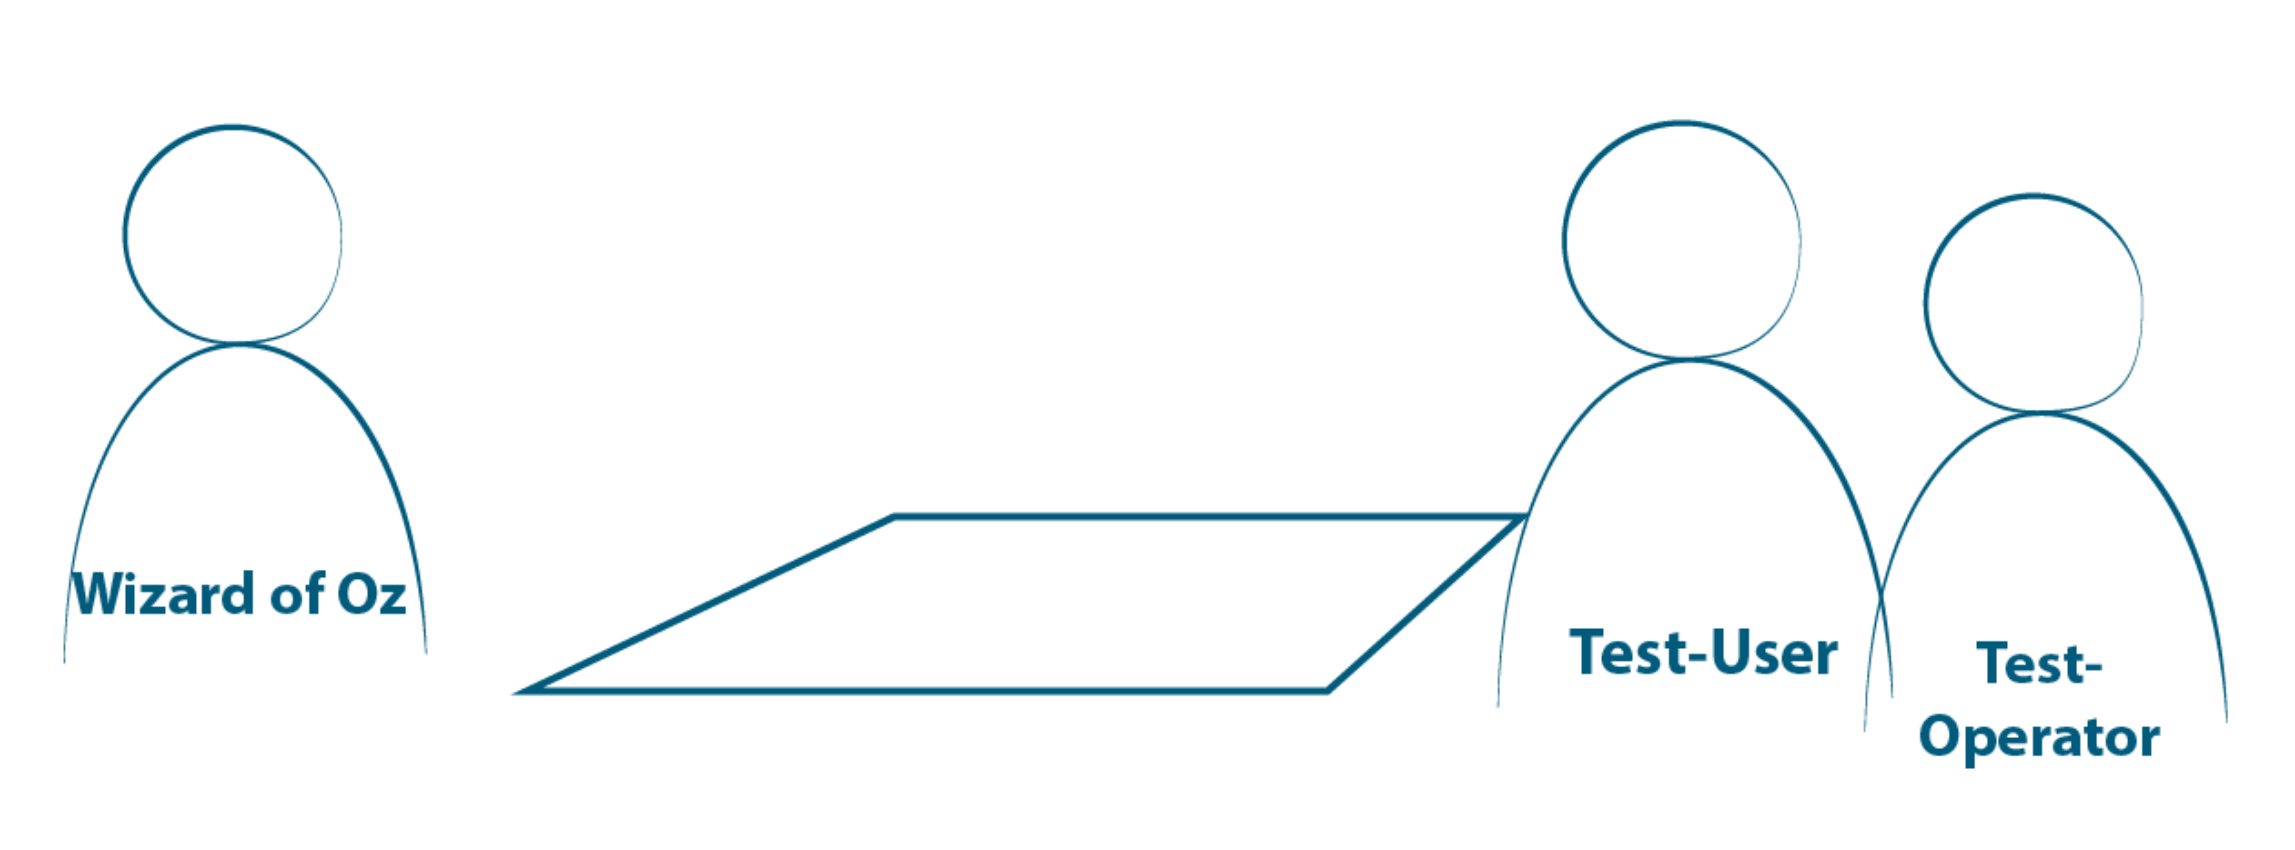
\includegraphics[width=0.75\textwidth]{bilder/WizardOfOz_v1.png}
    \caption{Einfaches Prototyping mit der \acl{WOz} Methode}
    \label{fig:wizard-of-oz-v1}
\end{figure}

Dabei sitzt der \acl{WOz} auf der einen, der Test-User und Test-Operator auf der anderen Seite eines Tisches. Der Operator moderiert das Szenario und führt die Testperson durch die Aufgaben. Der User bearbeitet die Aufgaben und sendet seine Anfragen an den \ac{WOz}, der diese nach einem zuvor definierten Ablaufszenario beantwortet. Der Operator kann währenddessen Notizen über die Testdurchführung machen.

Der große Nachteil bei einer Durchführung an diesem Aufbau ist, dass sich alle Beteiligten gegenseitig sehen und hören können. Der \acl{WOz} bekommt also sowohl die Kommunikation zwischen Test-User und Test-Operator, als auch deren Gestiken und Mimiken mit. Er könnte das System durch diese weiteren Informationskanäle daher anders bedienen, als er es bei einer reinen Textanfrage tun würde. Dieses Problem gilt gleichermaßen auch umgekehrt. Wenn die Testperson den \ac{WOz} sieht und realisiert, dass die Antworten von ihm kommen ist die Illusion von der Interaktion mit einem intelligenten System zerstört. \cite{bluemm_designing_2017} 

Diese Probleme lassen sich beheben, wenn der \acl{WOz} in einen Raum, Test-User und Test-Operator in einen anderen Raum platziert werden (siehe Abbildung \ref{fig:wizard-of-oz-v2}).
\newline

\begin{figure}[htb]
    \centering
    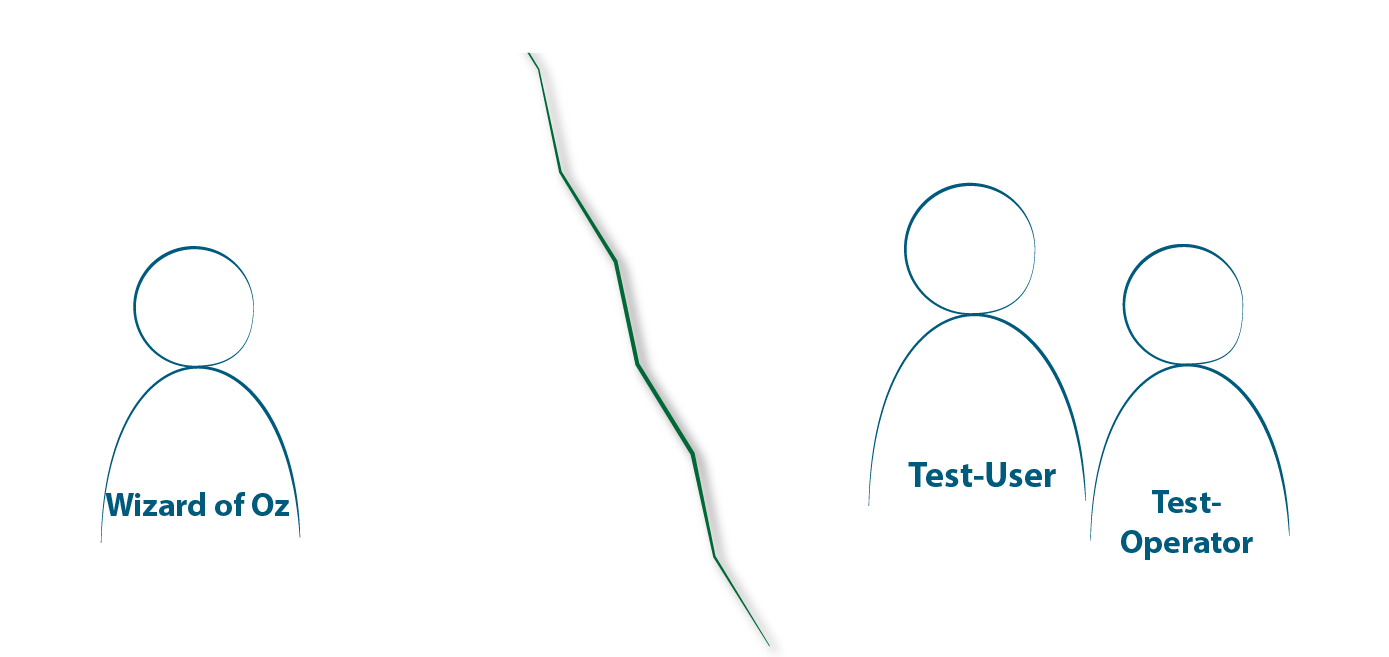
\includegraphics[width=0.75\textwidth]{bilder/WizardOfOz_v2.png}
    \caption{Erweitertes Prototyping mit der \acl{WOz} Methode}
    \label{fig:wizard-of-oz-v2}
\end{figure}

Im einfachsten Fall könnte dies mit Hilfe eines \textit{Chat Messengers}, wie z.B. Slack umgesetzt werden. User und Operator sitzen dazu in einem Raum, der \ac{WOz} in einem anderen. Beide haben jeweils ein Fenster des Chat Messengers geöffnet, wodurch sie ihre Nachrichten austauschen können. Die prinzipiellen Anforderungen an getrennte Räume und der Möglichkeit zum Textnachrichten-Austausch sind damit gegeben. Problematisch wird in diesem Zusammenhang aber die Chat-Umgebung an sich. Zunächst könnte der User erkennen, dass es sich um eine standardmäßige Messaging Platform handelt und die Illusion vom intelligenten Chatbot zerstören. Weiterhin sind die Möglichkeiten zur \ac{UI}-Erweiterung begrenzt, wodurch nur ein Bruchteil des Funktionsumfangs getestet werden könnte. Diese Nachteile sollen im nächsten Schritt egalisiert werden.  

Der Test-User soll nun eine prototypische Benutzeroberfläche an einem Rechner bedienen. Seine Eingaben sendet er dabei über eine Netzwerkverbindung direkt an den \ac{WOz}. Nachdem dieser ein Mensch ist, versteht er alle Intentionen des Nutzers und kann diese entsprechend zuordnen. Dabei geht er nach festgelegten Regeln vor und sendet die Antworten zurück an den User. Diese Antworten tippt er nicht selbst, sondern bedient sich dabei an vorgefertigten Phrasen, Textpassagen oder \ac{UI}-Elementen. Diese unterscheiden sich dabei je nach Szenario oder Intention des Nutzers. Bei einer übersichtlichen Gestaltung der Benutzeroberfläche findet sich der \acl{WOz} auch bei komplexen Tests zurecht. 

\subsection{Prototyping Tool}
\label{subsec:prototyping-tool}

Um all diese Anforderungen umsetzen zu können, wird ein \textit{\ac{cpt}} verwendet\footnote{Die Arbeit im Prototyping Tool stammt vom \ac{CUI}-Team der \adorsys\ unter der Leitung von Steffen Blümm}. Umgesetzt wird dies mit \textit{Max} von \textit{Cycling74}. Max ist eine grafische Entwicklungsumgebung, in der Module in einer Art \textit{Baukastensystem} verbunden werden. Die Entwicklung und Implementierung in diesem Zusammenhang ist nicht Bestandteil dieser Arbeit und soll daher nicht weiter beschrieben werden. Das Prototyping-System wird im Rahmen der Arbeit zur konzeptionellen Überprüfung der Konversationsstruktur und der \ac{UI}-Elemente genutzt. Wichtig zu erwähnen ist in diesem Zusammenhang, dass es gemäß der vorherigen Überlegungen zwei Benutzeroberflächen (Panels) gibt. Eine der Benutzeroberflächen bedient der \acl{WOz}, die andere der Test-User. Wie bereits zuvor festgelegt, befinden sich die jeweiligen Rechner in verschiedenen Räumen und tauschen ihre Daten über eine Netzwerkverbindung aus. 
\newline

\begin{figure}[H]
    \centering
    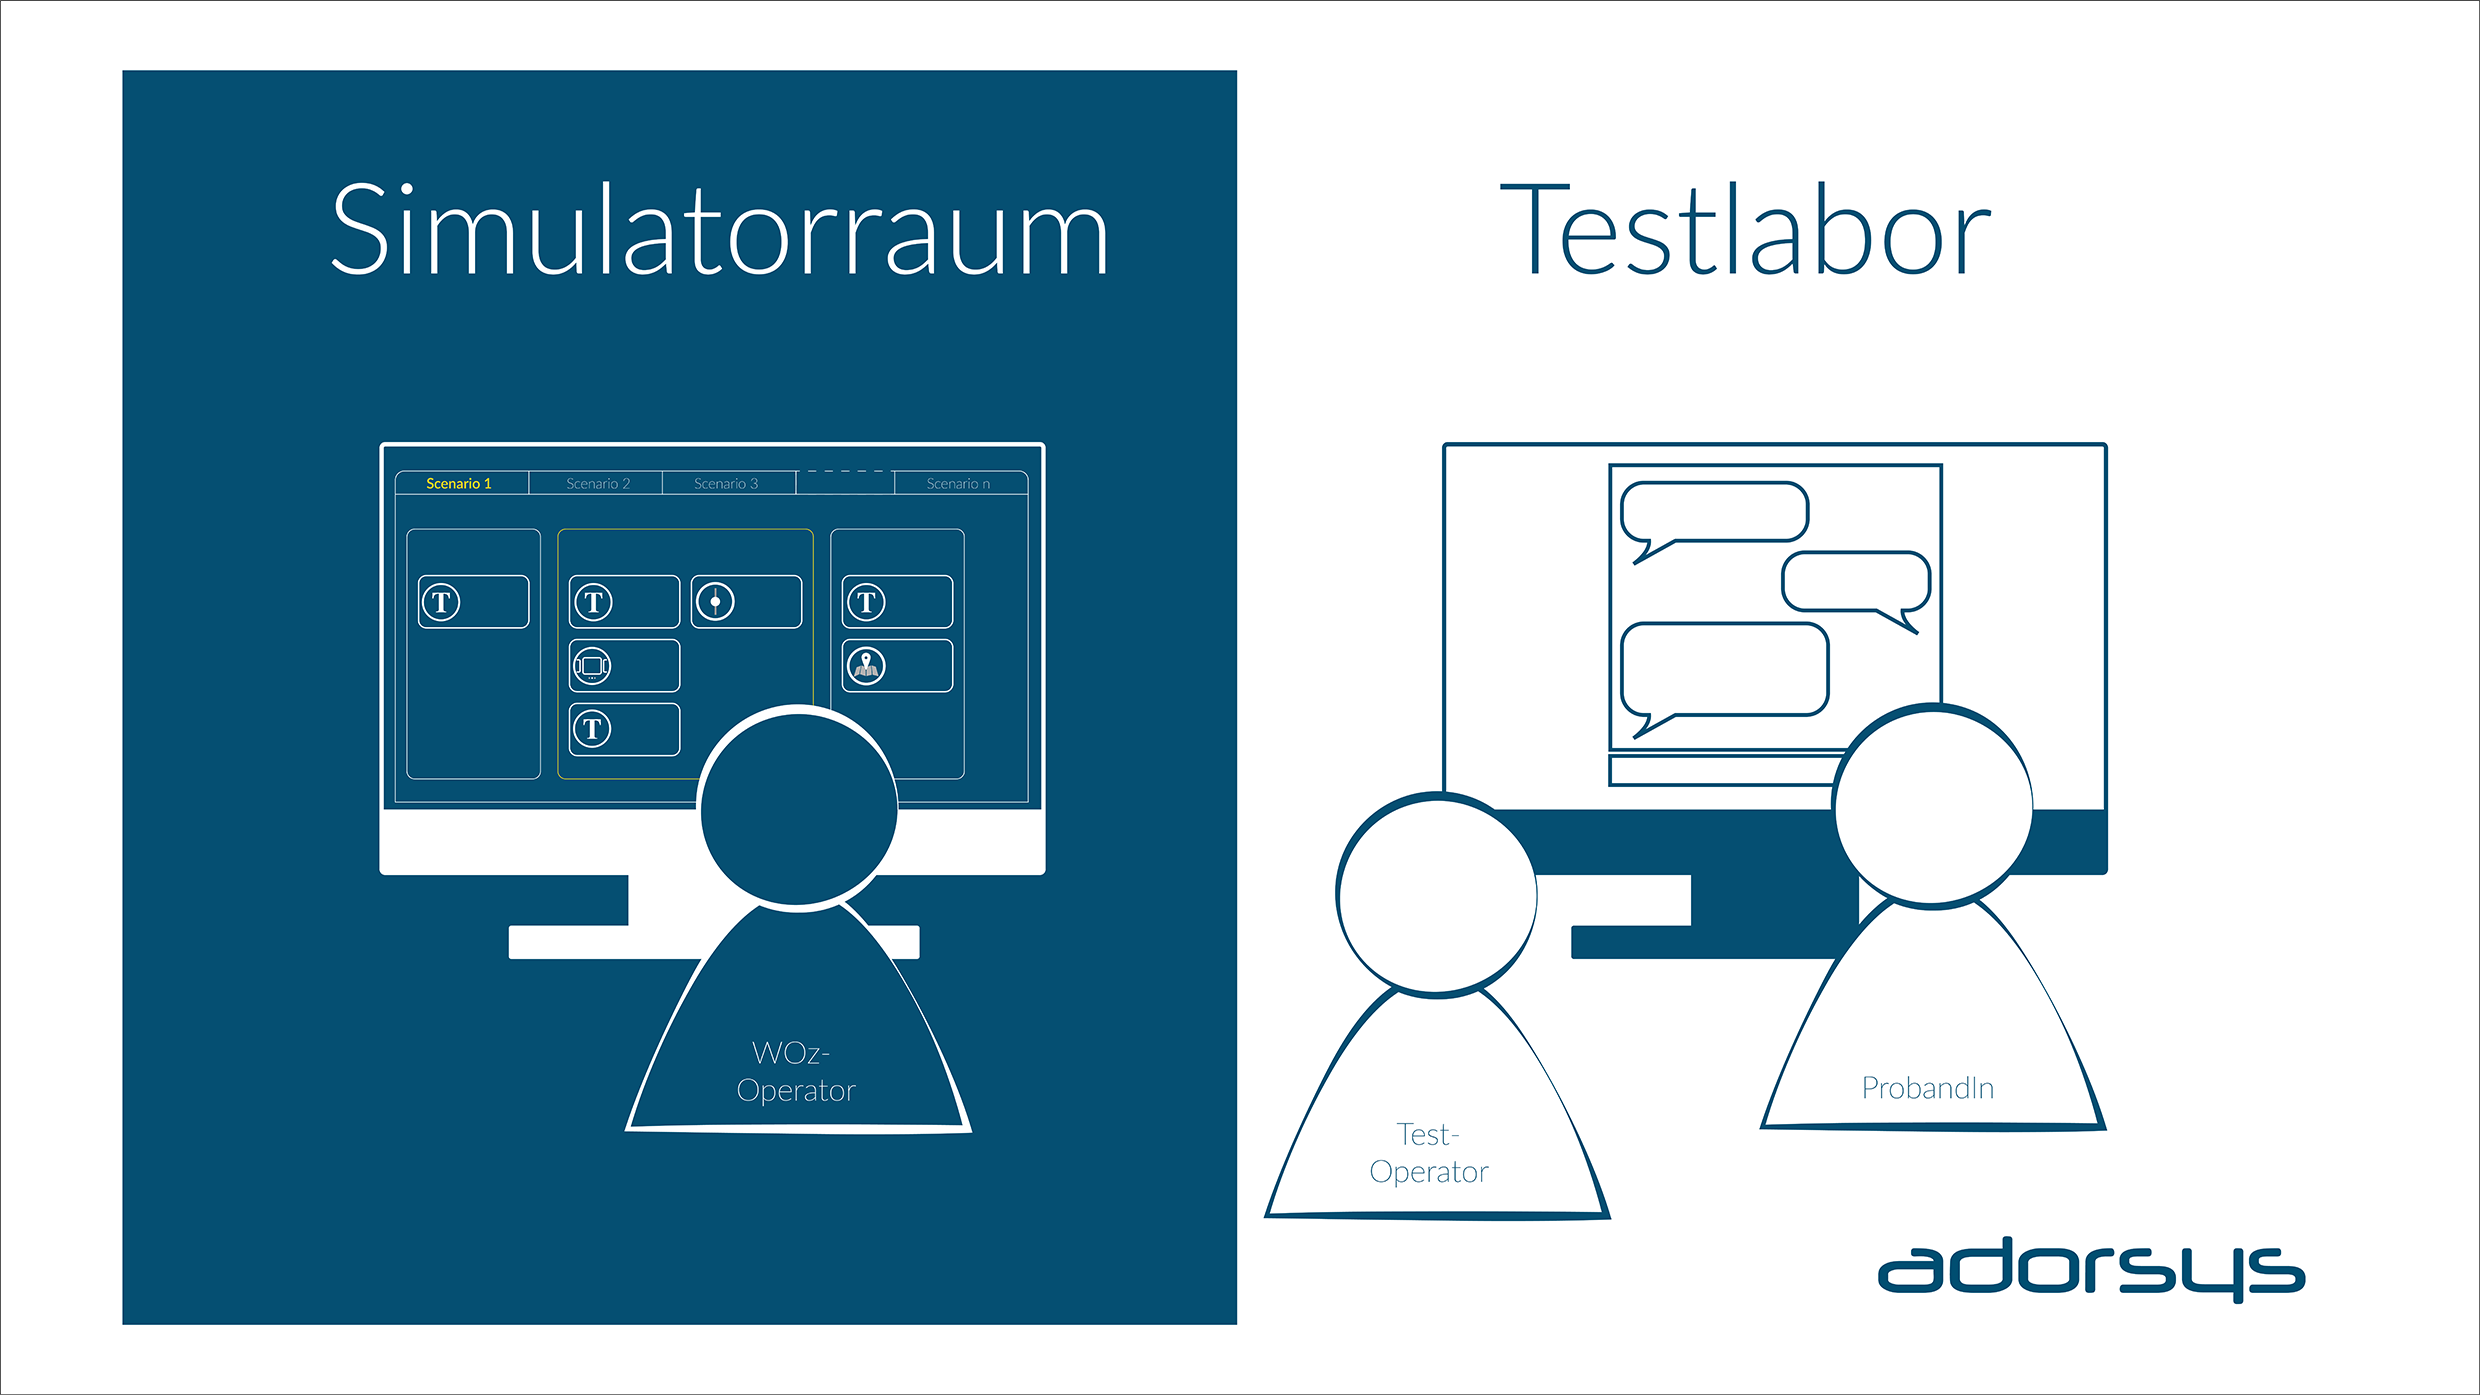
\includegraphics[width=0.75\textwidth]{bilder/WizardOfOz_v3.png}
    \caption{Komplettaufbau des Prototypings mit der Wizard of Oz Methode}
    \label{fig:wizard-of-oz-v3}
\end{figure}

Mit dem \textit{Tester-Panel} interagiert in der Regel nur der Test-User. Es ist dafür zuständig, dass die vom Nutzer eingegebenen Textanfragen übertragen werden. Seine Textnachrichten kann der User über die dunkelgraue Leiste am unteren Rand eingeben und abschicken. Außerdem gibt dieses Panel die vom \acl{WOz} generierten Antworten aus. Diese können, wie schon im vorherigen Teil der Arbeit beschrieben, sowohl Textnachrichten als auch erweiterte \ac{UI}-Elemente sein. Ziel dieser prototypischen User-Tests ist herauszufinden, welche erweiterten \aclp{UI} für den Nutzer verständlich sind und ihn bei der Raumbuchung unterstützen. Die entsprechenden \ac{UI}-Elemente können dann interaktiv bedient werden. Ein beispielhafter Ausschnitt des Tester-Panels ist in Abbildung \ref{fig:tester-panel} dargestellt. Eine ausführliche Darstellung aller \ac{UI}-Elemente befindet sich aus Gründen der besseren Lesbarkeit im Anhang \ref{sec:anhang-ui-elemente-prototyping}.
\newline

\begin{figure}[H]
    \centering
    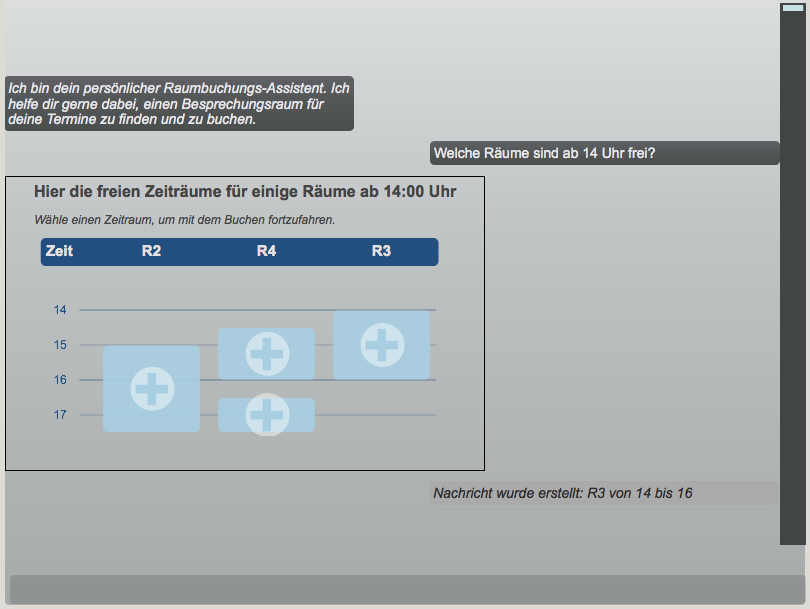
\includegraphics[width=0.8\textwidth]{bilder/TesterPanel.png}
    \caption{Grafische Benutzeroberfläche des Tester-Panels}
    \label{fig:tester-panel}
\end{figure}

Der \ac{WOz} sitzt während der Durchführung vor dem \textit{Simulator-Panel}. Diese Benutzeroberfläche kann gemäß eines vorher definierten Szenarios dynamisch aufgebaut werden. Dabei kann auf vordefinierte Phrasen oder \ac{UI}-Elemente zurückgegriffen werden. Zudem blinkt ein kleiner Kreis oben links, sobald der User auf der Tastatur tippt. Sendet er eine Nachricht ab, erscheint diese ebenfalls in der oberen linken Ecke. Durch das Triggern der Nachrichten wird Zeit gespart, da der \ac{WOz} nicht jede Antwort selbst generieren und formulieren muss. Außerdem ist so die Möglichkeit gegeben, dass jeder User innerhalb eines bestimmten Szenarios die gleichen Antworten und Formulierungen erhält, wodurch eine Verfälschung der Testergebnisse verhindert wird. Die Benutzeroberfläche des Simulator-Panels ist in Abbildung \ref{fig:simulator-panel} dargestellt.
\newline

\begin{figure}[H]
    \centering
    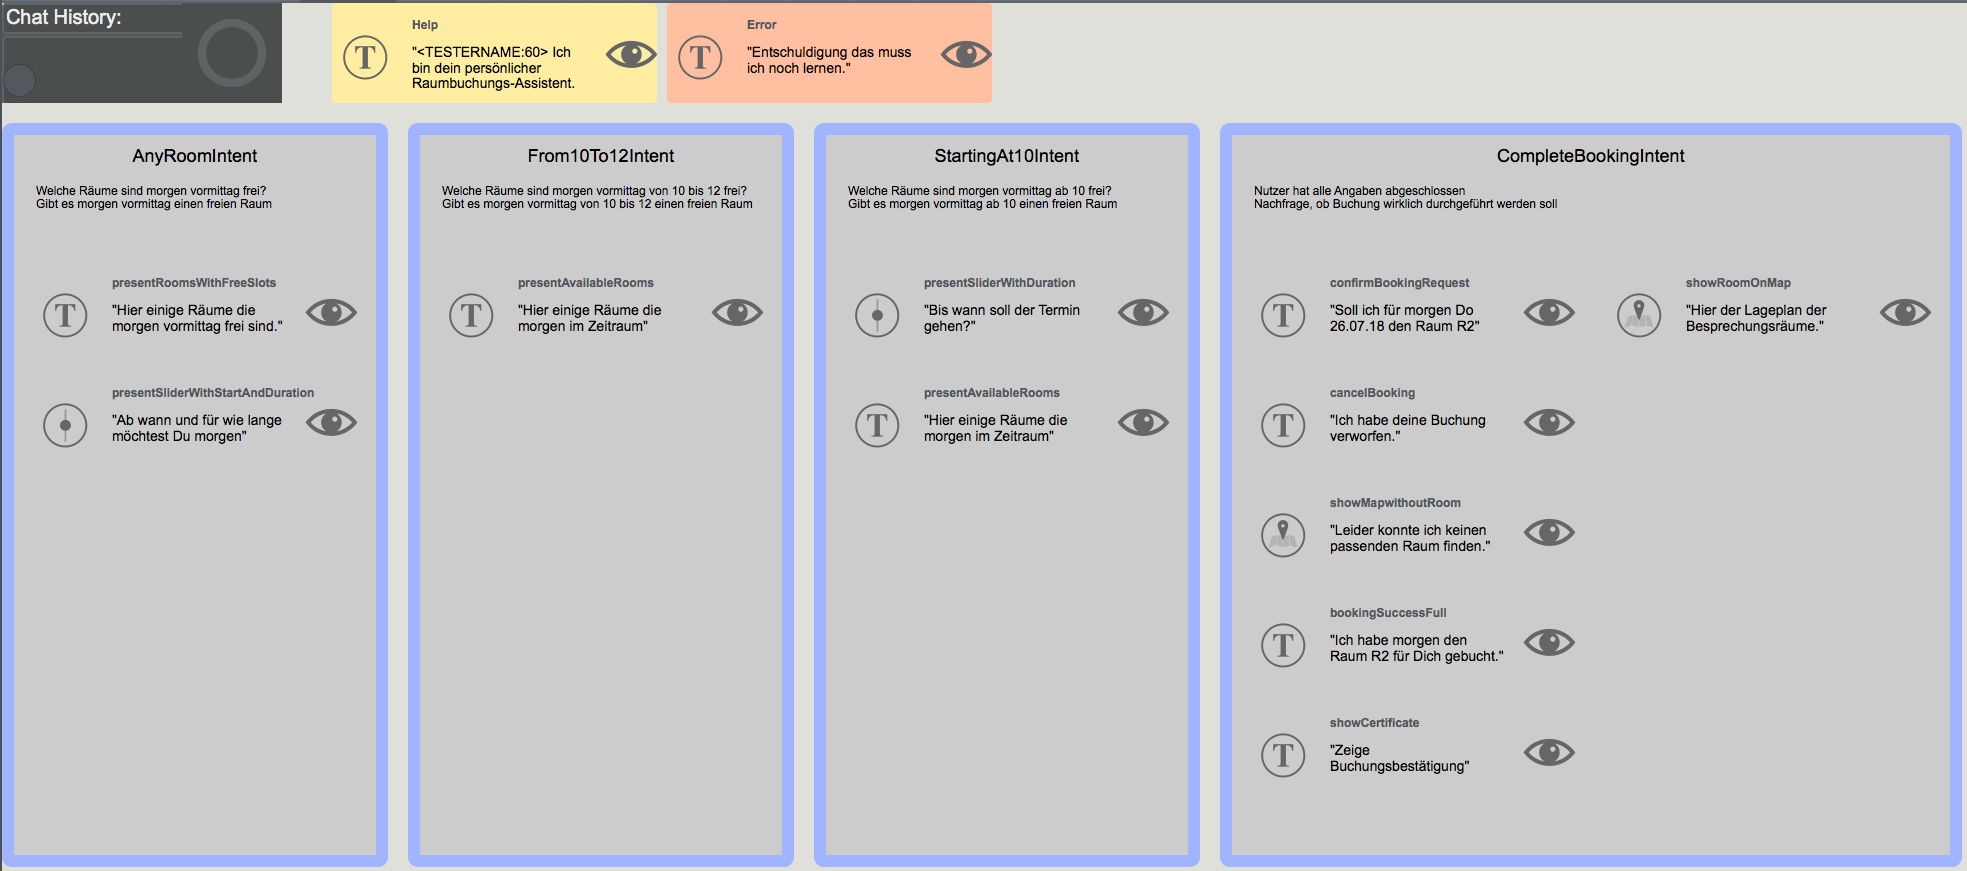
\includegraphics[width=1.0\textwidth]{bilder/simulator-panel.png}
    \caption{Grafische Benutzeroberfläche des Simulator-Panels}
    \label{fig:simulator-panel}
\end{figure}

Um ein \textit{Szenario} mit den verschiedenen Intents und Responses zu erstellen, wird eine Art \textit{Skript} verwendet. Dieses Skript wird im Format \textit{\ac{JSON}} geschrieben und enthält die entsprechenden Elemente in strukturierter Form. Für jedes Szenario gibt es dabei einen eigenen Tab (Tabs sind nicht in der Abbildung \ref{fig:simulator-panel} ersichtlich). 

Innerhalb jedes Szenarios können dann \textit{Intents} (blaue Rahmen) angelegt werden. Die ersten beiden Intents jedes Szenarios heißen \textit{helpIntent} und \textit{errorIntent}. Diese sind zum Schnellzugriff in der oberen Leiste (gelbes und oranges Feld) und triggern einfache Textnachrichten. Jeder Intent ist gleichermaßen aufgebaut und enthält die Parameter \textit{name}, \textit{utterances} und \textit{responses} (siehe Abbildung \ref{fig:json-structure}). 

Mit dem Parameter \textit{name} kann dem Intent ein Überbegriff zugeordnet werden. Unter \textit{utterances} können einige Beispielsätze des Users aufgezählt werden, die dem Operator das Bedienen erleichtern. Der letzte Parameter \textit{responses} kann je nach Art der Nachricht sehr umfangreich werden. 

Jede Response hat einen Parameter \textit{subject}, mit dem ihr ein Name zugeordnet werden kann. Mit Hilfe einer \textit{phrase} wird angegeben, welche Textnachricht an den User gesendet wird. Mit einem \textit{hint} kann dieser Text darunter zusätzlich in kleinerer Schrift ergänzt werden. Die Werte für \textit{type} und \textit{tags} ordnen der Response ein entsprechendes \ac{UI}-Element zu. Dabei gibt es verschiedene Elemente, wie z.B. eine \textit{CalendarView}, eine \textit{CollectionView} oder unterschiedliche \textit{Slidebars}. Mit Hilfe des Parameters \textit{payload} können dann zusätzliche Informationen über Startzeit, Dauer, Datum oder Raumname mitgegeben werden. An dieser Stelle soll aus Gründen der Übersichtlichkeit auf eine umfangreiche Darstellung verzichtet werden. Stattdessen ist nachfolgend zur beispielhaften Darstellung der Struktur einer Response die Implementierung einer kurzen \textit{Textmessage} in Listing \ref{lst:szenario-json} dargestellt. 
\newline

\begin{figure}[H]
    \centering
    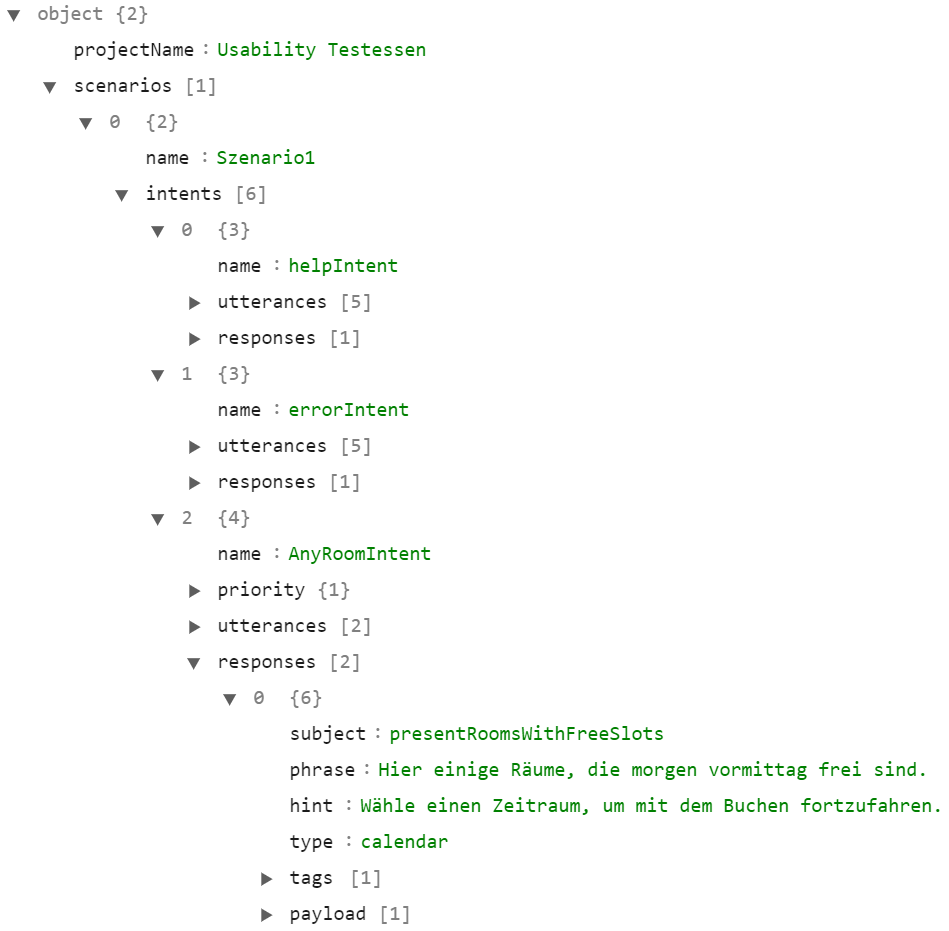
\includegraphics[width=1\textwidth]{bilder/json-structure-v2.PNG}
    \caption{Struktur eines Szenarios im \acs{JSON}-Format}
    \label{fig:json-structure}
\end{figure}
\clearpage
\begin{lstlisting}[caption={Beispielhafte Response im \acs{JSON}-Format}, captionpos=b, label={lst:szenario-json}, language=myjson]
{
    "responses": [
    {
        "subject": "Help",
        "phrase": "Ich bin dein persoenlicher Raumbuchungs Assistent. Ich helfe dir gerne dabei, einen Besprechungsraum fuer deine Termine zu finden und zu buchen.",
        "type": "textmessage"
    }]
}

\end{lstlisting}

\subsection{Usability Testessen}
\label{subsec:usability-testessen}

Erste User Tests mit dem \textit{Prototyping Tool} konnten mit externen Nutzern im Rahmen eines so genannten \textit{Usability Testessens}\footnote{www.usability-testessen.org} durchgeführt werden. Bei dieser Veranstaltung bringen Entwickler ihre Prototypen, Websites oder Apps mit. Freiwillige, vom Produkt unabhängige Nutzer testen diese dann auf ihre Gebrauchstauglichkeit. Dies hat den Vorteil, dass die Nutzer in der Regel keinen Bezug zum Produkt haben und somit ein unvoreingenommenes und ehrliches Feedback abgeben. 

Die Veranstalter selbst bezeichnen das als \textit{Speedtesting}. Die Probanden testen die verschiedenen Produkte in sechs Runden à zwölf Minuten. Nach Ablauf einer Runde wandern die Tester zum nächsten Stand. Getestet wird dabei mit Hilfe der \textit{Thinking-Aloud-Methode}. Dabei wird der Teilnehmer während der Testsitzung angehalten zu äußern, was er gerade denkt oder fühlt. Die Methode liefert somit ein schnelles Feedback und hilft, Usability-Probleme zu identifizieren. Um sicherzustellen, dass keine Informationen verloren gehen, wird der User Test mit einem Aufnahmegerät aufgezeichnet. Eine entsprechende Einverständniserklärung wird jedem Teilnehmer vor Beginn des Tests zur Unterschrift vorgelegt. Diese ist im Anhang \ref{sec:anhang-einverstaendniserklaerung-feedback-ext} zu finden. 

Der Testdurchlauf besteht im Wesentlichen aus zwei Teilen. Zunächst wird der Proband gebeten, ein bestimmtes Szenario mit Hilfe des Protoyping Tools abzuarbeiten. Als Benutzeroberfläche steht ihm dabei das Tester-Panel (vgl. Abbildung \ref{fig:tester-panel}) zur Verfügung. Alle seine Anfragen werden über eine Netzwerkverbindung an den \acl{WOz} gesendet, der vordefinierte Antworten über das Simulator-Panel (vgl. Abbildung \ref{fig:simulator-panel}) auswählen kann. Dem Proband wird somit der Eindruck einer Interaktion mit einem intelligenten Chatbot vorgetäuscht, hinter dem in Wirklichkeit ein Mensch steckt. Während der Nutzer das Szenario bearbeitet, können dank der Thinking-Aloud-Methode wertvolle Notizen zu Wahrnehmung und Verhalten des Nutzers gemacht \mbox{werden}. 

\begin{tikzpicture}
\node [mybox] (box){%
    \begin{minipage}{0.95\textwidth}
        Beschreibung:\\
        \textit{„Du willst morgen Vormittag um 10 Uhr an einem Meeting (Skype) teilnehmen, das bis zu 2 Stunden dauern kann. Die Videokonferenz findet an deinem eigenen Rechner statt. Um deine Kollegen nicht zu stören, willst du nicht vom Arbeitsplatz, sondern von einem Besprechungsraum aus teilnehmen. }\\
        Aufgabe:\\
        \textit{Lasse dir die verfügbaren Räume anzeigen und reserviere anschließend den Raum R2 von 10 bis 12 Uhr.“}
    \end{minipage}
};
\node[fancytitle, right=20pt] at (box.north west) { Szenario \textit{Usability Testessen} };
\end{tikzpicture}

Ist das Szenario erfolgreich abgeschlossen, wird der User noch gebeten, einen \textit{Feedback-Fragebogen} auszufüllen. Dieser besteht aus elf Gegensatzpaaren hinsichtlich der Wahrnehmung und Einstellung des Nutzers zum Produkt. Die Fragen sind dabei durch eine Skala mit fünf Auswahlmöglichkeiten zu beantworten. Eine Übersicht der Kriterien des Feedback-Fragebogens ist in der nachfolgenden Liste dargestellt.

\begin{itemize}
    \setlength{\itemindent}{0.5cm}
    \item verständlich $\longleftrightarrow$ unverständlich
    \item leicht zu erlernen $\longleftrightarrow$ schwer zu erlernen
    \item schnell $\longleftrightarrow$ langsam
    \item aufgeräumt $\longleftrightarrow$ überladen
    \item unterstützend $\longleftrightarrow$ behindernd
    \item angenehm $\longleftrightarrow$ unangenehm
    \item einfach $\longleftrightarrow$ kompliziert
    \item sympathisch $\longleftrightarrow$ unsympathisch
    \item erwartungskonform $\longleftrightarrow$ nicht erwartungskonform 
    \item effizient $\longleftrightarrow$ ineffizient 
    \item übersichtlich $\longleftrightarrow$ verwirrend 
\end{itemize}

Eine ausführliche Auflistung der Fragebögen mit Notizen zu den jeweiligen Teilnehmern befindet sich im Anhang \ref{sec:anhang-feedback-ext}. Die Inhalte und deren durchschnittliche Bewertung sind in Abbildung \ref{fig:diagram-auswertung-usability-testessen} anhand eines Diagramms dargestellt. Die gelbe Referenzlinie zeigt die durchschnittliche Bewertung des Systems durch alle Probanden. 
\newline

\begin{figure}[H]
    
  \begin{tikzpicture}

      \definecolor{myblue}{HTML}{0984bf} % Sekundäres adorsys blau
      \definecolor{myyellow}{HTML}{eed525} % adorsys gelb
      
      \draw (0cm,0cm) -- (13.2cm,0cm);  % Achse horizontal (Abzisse)
      \draw (0cm,0cm) -- (0cm,-0.1cm);  % linkes Ende der Abzisse
      \draw (13.2cm,0cm) -- (13.2cm,-0.1cm);  % rechtes Ende der Abzisse
      
      \draw (-0.1cm,0cm) -- (-0.1cm,10.5cm);  %Achse vertikal (Ordinate)
      \draw (-0.1cm,0cm) -- (-0.2cm,0cm);  % unteres Ende der Ordinate
      \draw (-0.1cm,10.5cm) -- (-0.2cm,10.5cm) node [left] {\%};  % oberes Ende der Ordinate
    
      % Hilfslinien bei 10, 20, ..., 90, 100 mit Beschriftung
      \foreach \x in {10,20,30,40,50,60,70,80,90,100}
        \draw[gray!50, text=black] (-0.2 cm,\x mm) -- (13.2 cm,\x mm) % Zeichnen der Hilfslinien
            node at (-0.5 cm,\x mm) {\x}; % Beschriftung der Hilfslinien
    
      % Gelber Strich, Avergave
      \draw[line width=0.5mm, myyellow] (-0.1 cm,80 mm) -- (13.1 cm,80 mm); % Zeichnen der Hilfslinien
      
      %\node at (6.7cm,11cm) {Zustimmung in Prozent};  %Überschrift
    
      \foreach \pos/\index in     {0.3/1,  % \pos ist Position der Säulen
                                  1.5/2,  % \index zählt bis 11 hoch
                                  2.7/3,
                                  3.9/4,
                                  5.1/5,
                                  6.3/6,
                                  7.5/7,
                                  8.7/8,
                                  9.9/9,
                                  11.1/10,
                                  12.3/11}
        {
        
        % Datensatz 'values' lesen -> Aus Index das jeweilige Kriterium und den Wert lesen
        \DTLassign{valuesTestEssen}{\index}{\kriterium=kriterium,\wert=wert}
        
         \draw[fill=myblue] (\pos cm,0cm) rectangle (0.6cm+\pos cm,\wert mm) % die Säulen
           node at (0.3cm + \pos cm,\wert mm + 0.3cm) {\wert}; %die Prozente über den Säulen
         \node[text=white, rotate=90, right] at (0.3 cm +\pos cm,0.5cm) {\textbf{\kriterium}}; %Säulenbeschriftung
        };
        
    \end{tikzpicture}
    \caption{Ergebnisse des Usability Testessens}
    \label{fig:diagram-auswertung-usability-testessen}
\end{figure}

Im Großen und Ganzen gaben die Probanden positives Feedback. Im Durchschnitt ergibt sich eine Zustimmung zum System von ca. 80\,\%. Insgesamt gibt es dabei keine allzu großen Diskrepanzen. Anzumerken ist, dass ein Großteil der Nutzer den Prototyp als \textit{angenehm} (88\,\%), \textit{verständlich} und \textit{schnell} (je 83\,\%) empfand. Etwas weniger, aber dennoch 75\,\% Zustimmung bekamen Kriterien wie \textit{aufgeräumt} oder \textit{übersichtlich}, was jedoch auch auf die prototypische Umgebung zurückzuführen sein kann. Anzumerken ist hierbei, dass aufgrund von begrenzter Zeit und Umfang dieser Testveranstaltung keine fundierte Aussage über qualitative oder funktionale Eigenschaften des Systems getroffen werden kann. Die Bewertung ist jedoch äußerst hilfreich, um ein erstes, schnelles Feedback der geplanten Applikation zu erhalten und hilft damit bei der weiteren Konzeption des Systems.

Die ersten Ergebnisse spiegeln sich auch mit einigen Zitaten der Probanden wider. \textit{„Wenn das bei uns so einfach funktionieren würde, wäre das schon toll.“} oder \textit{„Das hätte ich auch gerne, ich kenne das komplizerter.“} sind nur einige Zitate in diesem Zusammenhang. Daraus lässt sich ableiten, dass die Nutzer dem System grundsätzlich positiv gegenüberstehen und sowohl die Raumbuchung via Chatbot als auch die \ac{UI}-Erweiterungen verständlich sind. 

Von beinahe allen Probanden wurde außerdem erwähnt, dass das Feature \textit{Chatbot is thinking} hilfreich ist und den Chatbot obendrein sympathisch macht. Mit dieser Funktion wird die Zeit überbrückt, die der Chatbot für die Verarbeitung einer Nutzereingabe benötigt. Als negatives Feedback erwähnten einige User die farblichen Markierungen im Lageplan. Hier geht die farbliche Markierung des gebuchten Raumes gegenüber den anderen Symbolen unter. Abgesehen davon war der Lageplan jedoch hilfreich. Als Anmerkung nannten die Nutzer immer wieder die Frage nach der Ausstattung der Räume. Hier spielten vor allem die Fragen nach WLAN, Anzahl der Plätze, Whiteboard, Flipchart, Beamer, Getränke oder Catering eine Rolle. Zudem äußerten einige User den Wunsch, dass der gebuchte Termin anschließend automatisch in ihren elektronischen Kalender eingetragen werden soll.    

\subsection{Szenarien}
\label{subsec:szenarien}

Im Rahmen von ausführlichen User Tests werden verschiedene Szenarien, basierend auf die erdachten Personae aus \ref{subsec:personae}, entwickelt. Entsprechend den jeweiligen Bereichen Development, Coaching, Human Resources und Vertrieb wird jeweils ein spezifisches Szenario erstellt. Die Szenarien werden im Folgenden kurz vorgestellt und deren Hintergedanken beschrieben.

Das Szenario aus dem Bereich \textit{Development} ist an die Persona Heiko Neumann angelehnt. Heiko ist Softwareentwickler und möchte zusammen mit einem Kollegen ein spontanes Code-Review durchführen. Er hat dabei keine besonderen Ansprüche an einen Raum. Für seine Buchung wird die entsprechende Raumhierarchie aus \ref{tab:raum-priorisierung} \mbox{angewendet}. 

\begin{tikzpicture}
\node [mybox] (box){%
    \begin{minipage}{0.95\textwidth}
        Beschreibung: \\
        \textit{Du willst jetzt sofort (14:00 Uhr) ein Meeting (Code-Review) machen. Der Termin dauert mindestens eine halbe Stunde und findet mit einem weiteren Kollegen statt. Um ungestört arbeiten zu können, willst du einen beliebigen Besprechungsraum dafür buchen.} \\
        Aufgabe: \\
        \textit{Lasse dir die verfügbaren Räume anzeigen und reserviere anschließend den Raum R3 so, dass du ihn ab jetzt eine Stunde nutzen kannst.} \\
        Weitere Informationen: \\
        \textit{Titel für den Termin: Keinen Titel angeben}
    \end{minipage}
};
\node[fancytitle, right=20pt] at (box.north west) { Szenario \textit{Development} };
\end{tikzpicture}

Sandra Böhm ist die Persona aus dem Bereich \textit{Coaching}. Sie möchte einen interaktiven Scrum Workshop veranstalten. Aufgrund der Teilnehmerzahl von zwölf Personen benötigt sie dazu den Raum R6. Das System soll dabei erkennnen, dass es sich um einen ganztägigen Termin handelt und bei der Buchung, entsprechend der Idee aus \ref{subsec:interviews}, nach Vor- und Nachbereitungszeit für den Termin fragen. Wählt der User eine entsprechende Vor- und Nachbereitungszeit aus, nimmt das System direkt alle drei Buchungen vor und erleichtert dem Nutzer somit die Buchung von drei einzelnen Terminen. 

\begin{tikzpicture}
\node [mybox] (box){%
    \begin{minipage}{0.95\textwidth}
        Beschreibung: \\
        \textit{Du willst einen interaktiven Scrum Workshop halten. Daran werden etwa zwölf Leute teilnehmen, weshalb du den Raum R6 benötigst. Der Termin soll als ganztägiges Ereignis stattfinden. Die Kernzeit für alle Teilnehmer ist dabei von 9:00 Uhr bis 17:00 Uhr. Für dich selbst möchtest du jedoch zusätzlich je eine Stunde zur Vor- und Nachbereitung des Workshops buchen.} \\
        Aufgabe: \\
        \textit{Lasse dir die nächsten Termine anzeigen, an denen der Raum R6 ganztägig frei ist und reserviere ihn anschließend für den nächstmöglichen Zeitpunkt zu den oben stehenden Bedingungen.} \\
        Weitere Informationen: \\
        \textit{Titel für den Termin: „Scrum Workshop“}
    \end{minipage}
};
\node[fancytitle, right=20pt] at (box.north west) { Szenario \textit{Coaching} };
\end{tikzpicture}

Die Persona Michelle Färber repräsentiert den Bereich \textit{Human Resources}. In dem spezifischen Szenario möchte sie einen Raum für ein Vorstellungsgespräch buchen. Wird dem System entsprechend mitgeteilt, dass es sich um ein Vorstellungsgespräch handelt, ändert sich die Priorisierung der Räume. Räume, die Diskretion bieten, werden in diesem Fall höher priorisiert und zuerst vorgeschlagen. 

\begin{tikzpicture}
\node [mybox] (box){%
    \begin{minipage}{0.95\textwidth}
        Beschreibung: \\
        \textit{Du arbeitest im Bereich HR und möchtest einen Raum für ein Vorstellungsgespräch buchen. Du hast mit dem Bewerber einen Termin am nächsten Montag von 10:00 Uhr bis 11:30 Uhr vereinbart. Da du als HR-Mitarbeiter möchtest, dass der Bewerber sich wohlfühlt und möglichst ein gewisses Maß an Diskretion gegeben ist, ergibt sich für dich folgende Priorisierung der Räume: R4 (Diskretion, hell), R3 (Diskretion, dunkel), R1 (keine Diskretion, hell), R2 (keine Diskretion, hell). } \\
        Aufgabe: \\
        \textit{Reserviere den bestmöglichen Raum zu den oben genannten Bedingungen.}  \\
        Weitere Informationen: \\
        \textit{Titel für den Termin: „VG Java Entwickler“}
    \end{minipage}
};
\node[fancytitle, right=20pt] at (box.north west) { Szenario \textit{Human Resources} };
\end{tikzpicture}

Eric Schweizer steht für die Persona aus dem \textit{Vertrieb}. Er möchte für die kommende Woche ein Projektanbahnungsgespräch organisieren. Die Uhrzeit ist durch den Kunden fest vorgegeben. Er benötigt dazu keinen besonderen Raum. Für seine Buchung wird die entsprechende Raumhierarchie aus Tabelle \ref{tab:raum-priorisierung} angewendet. 

\begin{tikzpicture}
\node [mybox] (box){%
    \begin{minipage}{0.95\textwidth}
        Beschreibung: \\
        \textit{Du willst nächste Woche am Dienstag ein Projektanbahnungsgespräch organisieren. Zu dem Termin kommen neben dir noch ein Designer, der vorgesehene Projektmanager sowie drei Mitarbeiter des Kunden. Das Meeting soll um 9:30 Uhr beginnen und etwa 2-3 Stunden dauern.} \\
        Aufgabe: \\
        \textit{Lasse dir die verfügbaren Räume anzeigen und reserviere anschließend den Raum R1 von 9:30 Uhr bis 13:00 Uhr.} \\
        Weitere Informationen: \\
        \textit{Titel für den Termin: „Projektanbahnung VR Bank“}
    \end{minipage}
};
\node[fancytitle, right=20pt] at (box.north west) { Szenario \textit{Vertrieb} };
\end{tikzpicture}




\subsection{Workflow}
\label{subsec:workflow}

Zu den beschriebenen Szenarien werden User Tests durchgeführt. Der damit verbundene Workflow und die Grundüberlegungen sollen im Folgenden anhand eines spezifischen Szenarios erläutert werden. Für diesen Fall wird das Szenario aus dem Bereich \textit{Vertrieb} betrachtet. 

Um diese Aufgabe zu erledigen und den Raum R1 von 9:30 Uhr bis 13:00 Uhr zu reservieren, hat der Nutzer verschiedene Möglichkeiten. Diese sind in Abbildung \ref{fig:decision-tree-vertrieb} in Form eines Entscheidungsbaums (engl. \textit{decision tree}) dargestellt. Die einzelnen Zweige werden anschließend genauer erläutert.
\newline

\begin{figure}[H]
    \centering
    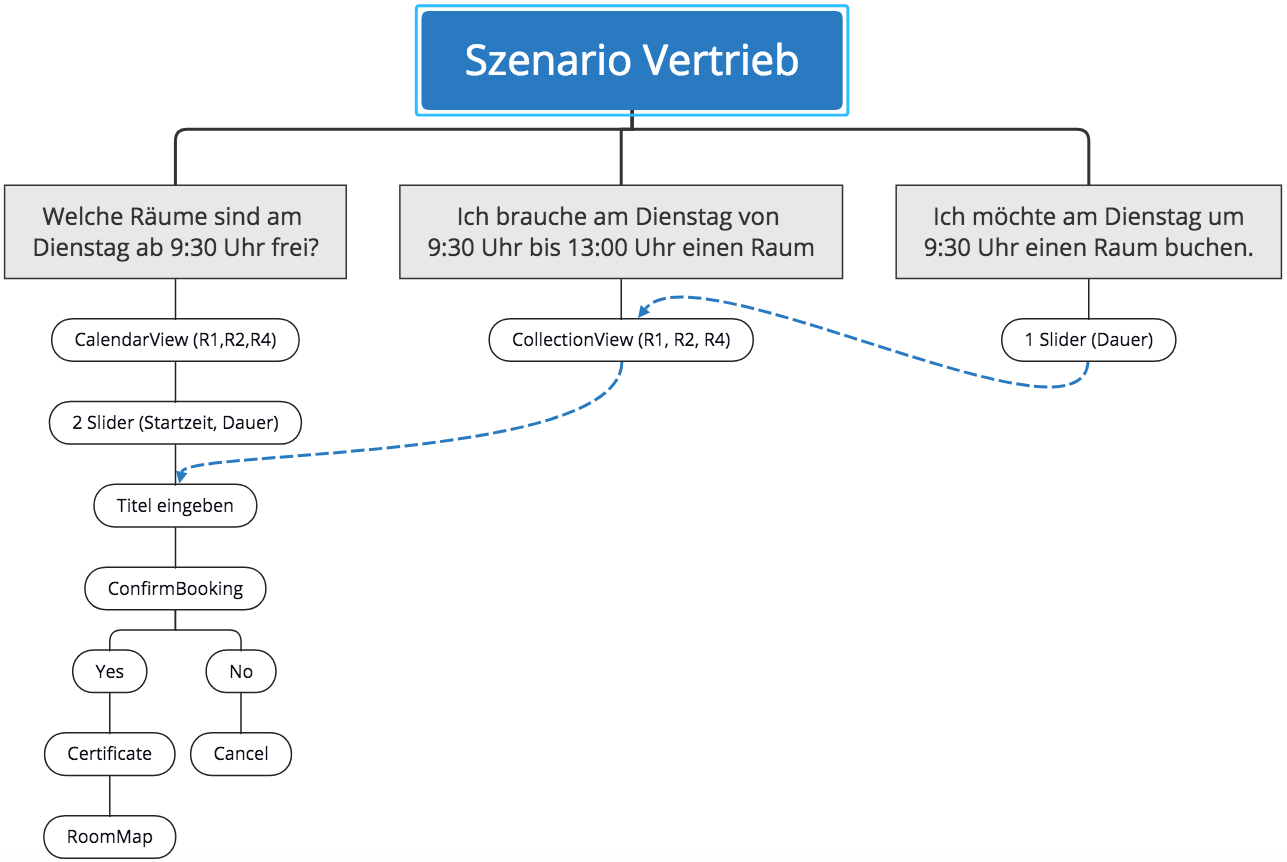
\includegraphics[width=0.9\textwidth]{bilder/SzenarioVertriebMindMap.png}
    \caption{Entscheidungsbaum zum Szenario \textit{Vertrieb}}
    \label{fig:decision-tree-vertrieb}
\end{figure}

Zunächst kann sich der Nutzer die ab 9:30 Uhr verfügbaren Räume anzeigen lassen (linker Zweig). Eine entsprechende Formulierung könnte so aussehen:

\begin{center}
    \textit{Welche Räume sind am Dienstag ab 9:30 Uhr frei?}
\end{center}

Das System zeigt daraufhin eine \textit{CalendarView} mit den verfügbaren Räumen. Der Nutzer wählt einen für seinen Zeitraum passenden Zeitslot aus und wird anschließend mit Hilfe von zwei \textit{Slidern} nach der Startzeit und Dauer seines Termins gefragt. Danach hat das System alle notwendigen Parameter und kann die Buchung nach Eingabe eines Titels abschließen.

Bei anderer Formulierung der Intention kann das System direkt erkennen, dass der Nutzer einen Raum von 9:30 Uhr bis 13:00 Uhr benötigt (mittlerer Zweig). Diese Formulierung könnte beispielsweise so lauten:

\begin{center}
    \textit{Ich brauche am Dienstag von 9:30 Uhr bis 13:00 Uhr einen Raum.}
\end{center}

Das System erkennt direkt den Start- und Endzeitpunkt des Termins und kann die verfügbaren Räume mit Hilfe einer \textit{CollectionView} anzeigen. Wählt der Nutzer einen Raum aus, hat das System alle notwendigen Parameter und kann mit der Eingabe des Titels fortfahren. 

Ist die Formulierung ähnlich, beinhaltet allerdings nur den Startzeitpunkt von 9:30 Uhr für den Termin, kann mit einem kleinen Umweg genauso vorgegangen werden (rechter Zweig). Eine Möglichkeit der Formulierung wäre:

\begin{center}
    \textit{Ich möchte am Dienstag um 9:30 Uhr einen Raum buchen.}
\end{center}

Das System fragt den Nutzer über einen \textit{Slider} nach der Dauer des Termins. Hat der User diese eingegeben, kann auf gleiche Art und Weise vorgegangen werden. Der Raum wird über eine \textit{CollectionView} ausgewählt und die Buchung anschließend \mbox{abgeschlossen}. 

Der Abschluss einer Buchung trifft sich für alle möglichen Zweige an einem Punkt wieder. In diesem Szenario ist das die Stelle, an der die \textit{Eingabe des Titels} erfolgt. Im Rahmen der Arbeit wird eine Festlegung zur Angabe von Titeln bei Terminen getroffen. Ab einer Dauer des Termins von 1,5 Stunden muss ein Termin einen Titel haben. Dauert der Termin weniger als 1,5 Stunden, kann der Nutzer optional und auf eigenen Wunsch einen Titel hinzufügen. Tut er dies nicht, wird ein automatisch generierter Titel mit dem Namen des Organisators eingetragen. Anschließend wird die Buchung noch über das \ac{UI}-Element \textit{ConfirmBooking} abgeschlossen.
\clearpage
Der \acl{WOz} hat die in \ref{subsec:prototyping-tool} beschriebene Operator-Ansicht. Die Zweige des oben beschriebenen Entscheidungsbaums sind in Abbildung \ref{fig:operator-screen-vertrieb} als blaue Kästen wieder zu finden. 
\newline

\begin{figure}[H]
    \centering
    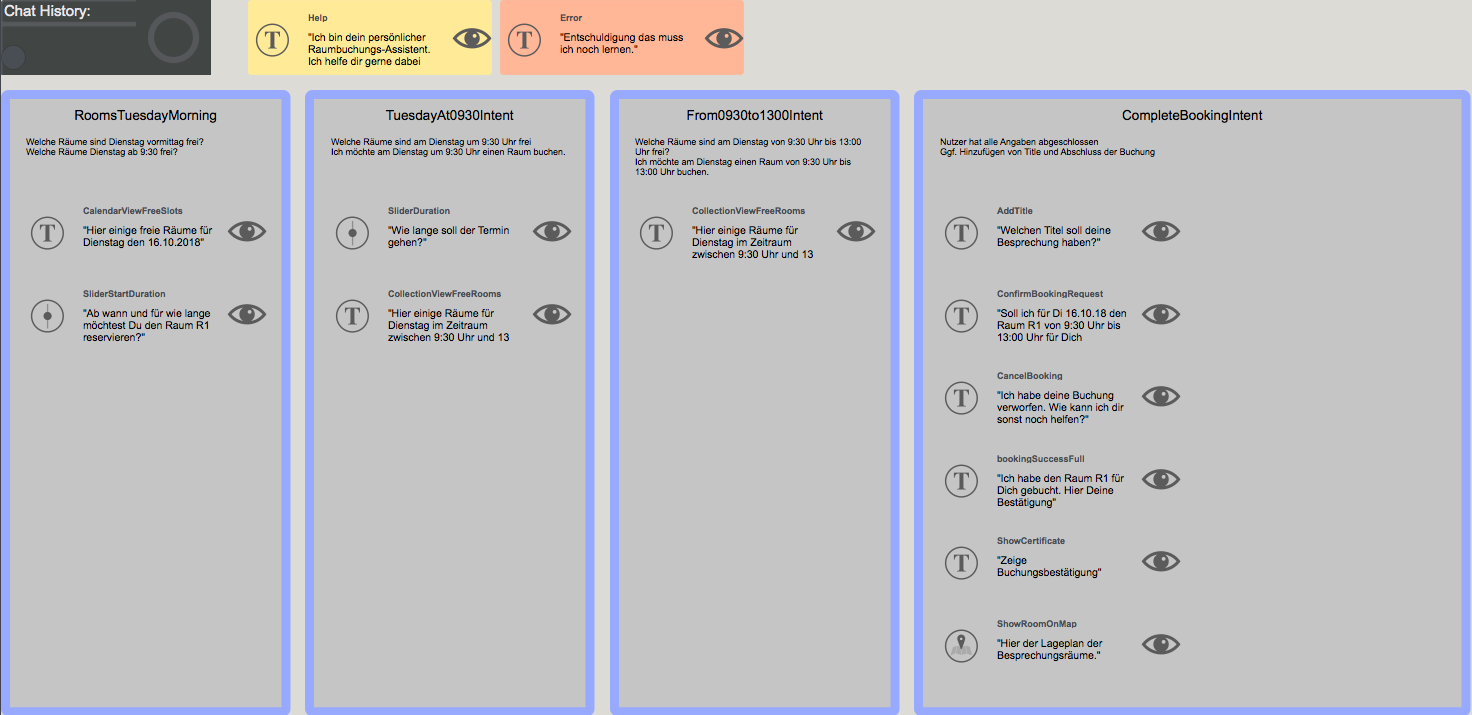
\includegraphics[width=1.0\textwidth]{bilder/OperatorSzenarioVertrieb.png}
    \caption{Benutzeroberfläche des Operators zum Szenario \textit{Vertrieb}}
    \label{fig:operator-screen-vertrieb}
\end{figure}

Die linken drei Kästen können entsprechend von oben nach unten abgearbeitet werden. Danach befindet sich der Knotenpunkt zur Eingabe des Titels. Ab hier ist der Ablauf für alle Fälle gleich, wonach der rechte blaue Kasten von oben nach unten durchlaufen wird. 

Der Test-User bekommt von all dem nicht viel mit. Er bearbeitet das Szenario und wählt eine für ihn passende Formulierung aus. Über die Benutzeroberfläche des Tester-Panels interagiert er mit dem System und erhält entsprechende Rückmeldungen in Form von Text oder \ac{UI}-Elementen. Ein möglicher Durchlauf aus der Sicht des Probanden ist in Abbildung \ref{fig:test-user-screen-vertrieb} dargestellt.
\newline

\begin{figure}[H]
    \centering
    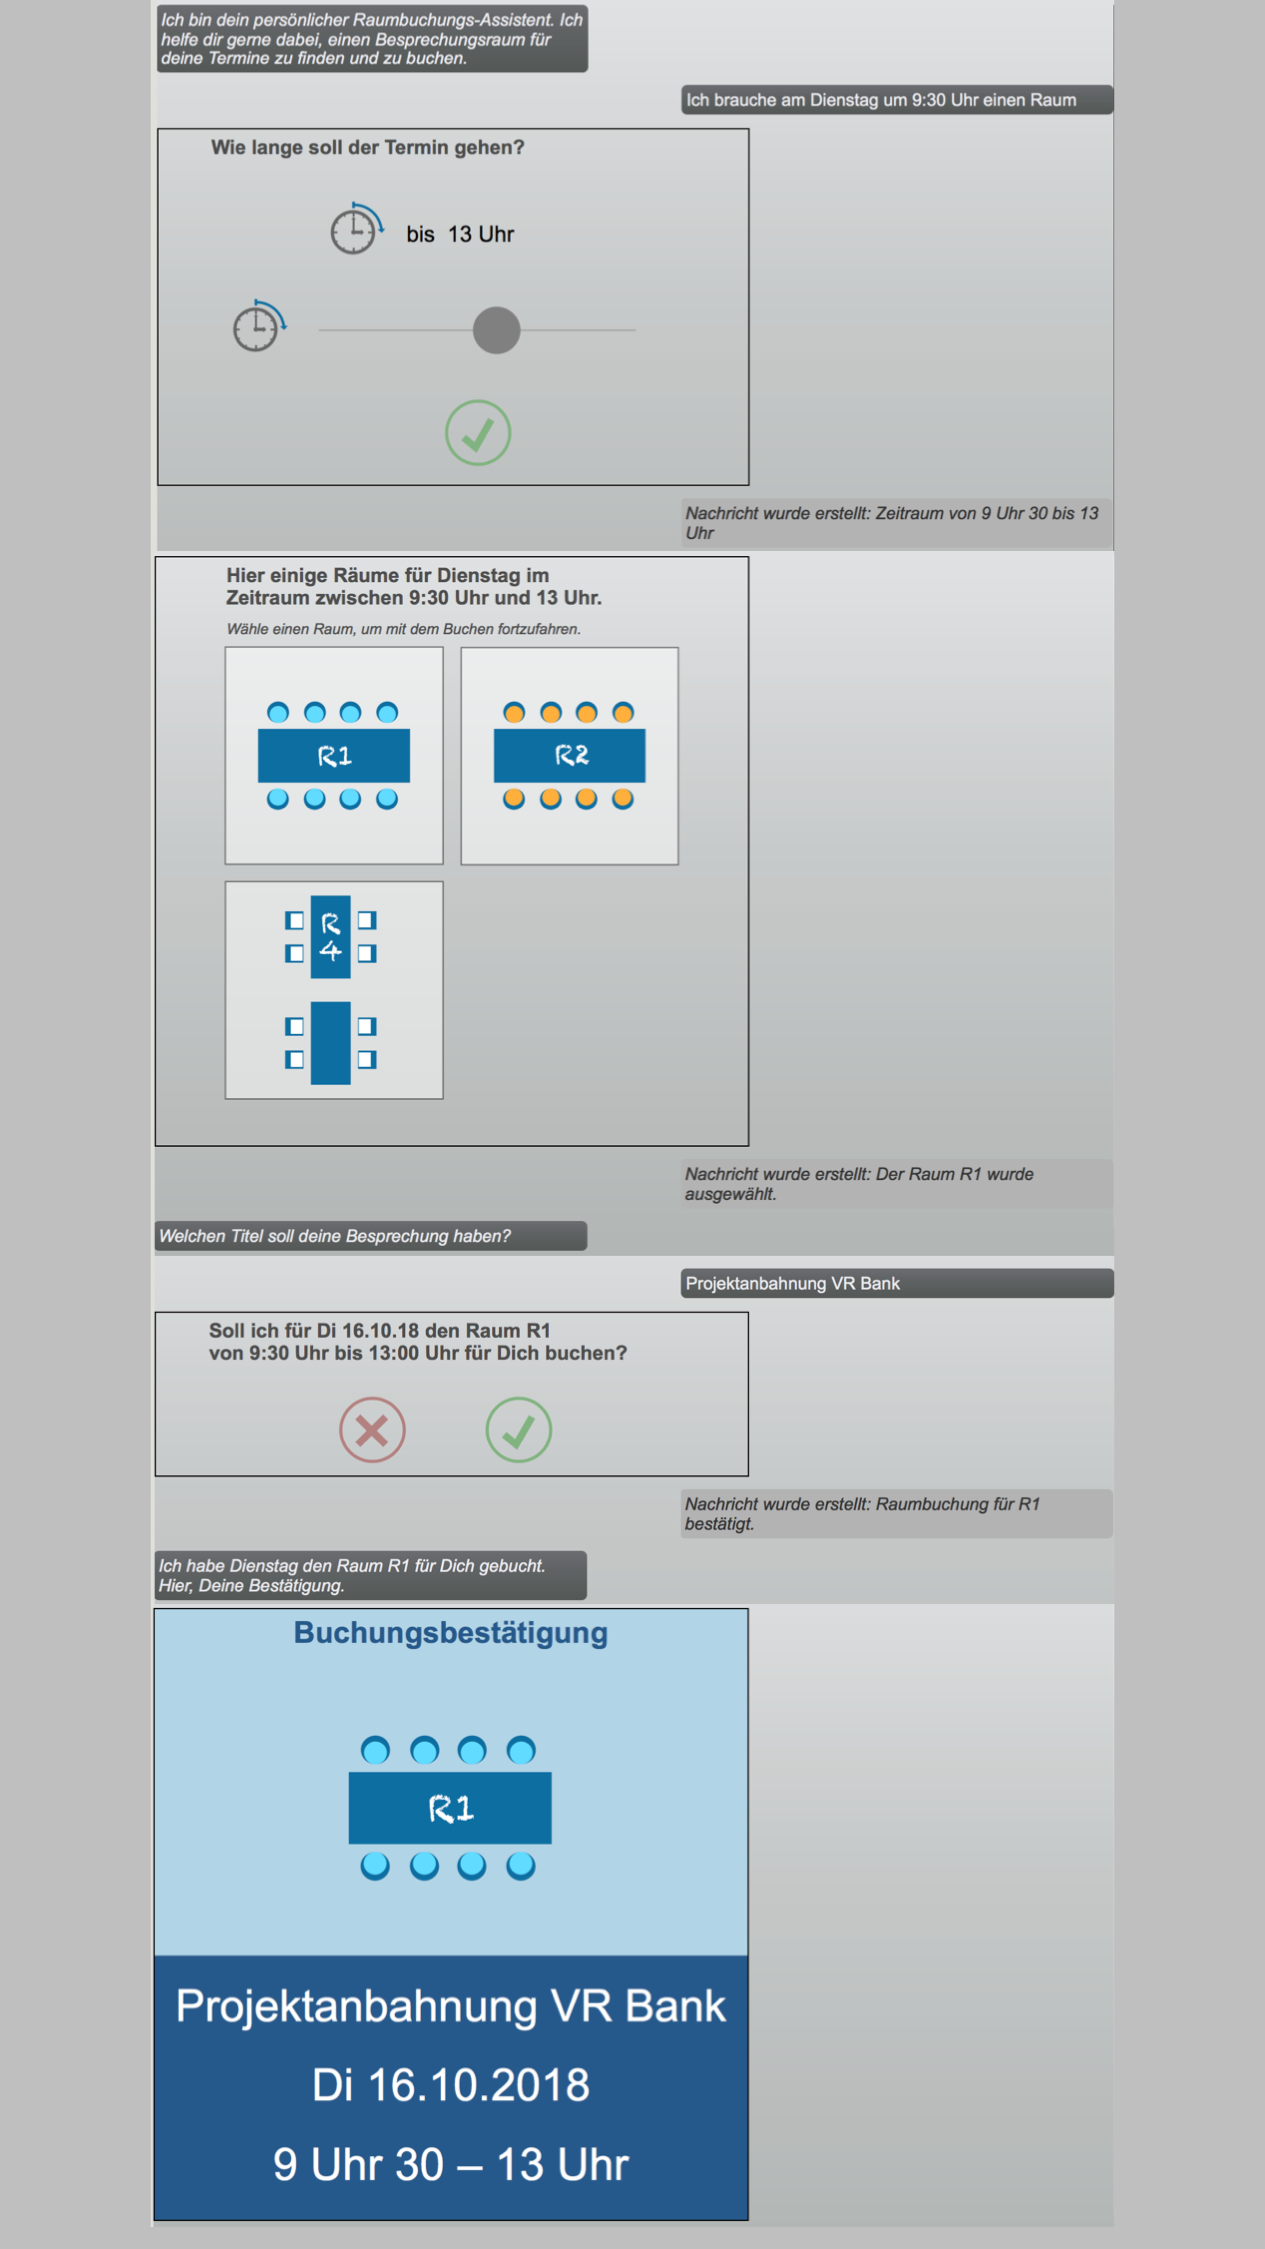
\includegraphics[width=0.85\textwidth]{bilder/WorkflowTesterPanel.png}
    \caption{Benutzeroberfläche des Probanden zum Szenario \textit{Vertrieb}}
    \label{fig:test-user-screen-vertrieb}
\end{figure}

\subsection{User Tests}
\label{subsec:user-tests}

Zur Evaluierung der konzeptionellen Überlegungen werden abschließend User Tests durchgeführt. Grundsätzlich sollen dabei Parallelen zu den ersten Tests im Rahmen des Usability Testessens (siehe \ref{subsec:usability-testessen}) gezogen werden können. Daher wird der Prototyp auch in diesem Fall von sechs Probanden getestet. Aufgrund der intensiveren Betrachtungen im Kontext des Requirements Engineering in Form von Fragebögen, Interviews oder der Entwicklung von Personae fällt der Test in diesem Fall umfangreicher aus. Die Probanden bearbeiten jedes der in \ref{subsec:szenarien} definierten Szenarien als eigenständige Aufgabe. Auch hier wird wieder die \textit{Thinking-Aloud-Methode} angewendet und der User Test mit einem Aufnahmegerät aufgezeichnet. Dazu wird die entsprechende Einverständniserklärung aus Anhang \ref{sec:anhang-einverstaendnis-user-test} verwendet. 

Nach der Begrüßung und Unterschrift der Einveständniserklärung bearbeitet der Proband die vier Szenarien in einer zuvor festgelegten Reihenfolge. Nachdem die Nutzer bereits nach wenigen Arbeitsschritten die Bedienung des Systems erlernen, werden die Szenarien unterschiedlich angeordnet, um so eine Verfälschung der Ergebnisse auszuschließen. Dazu werden die vier Szenarien für die User mit Hilfe eines Online-Tools randomisiert \cite{jumk.de_generator_2018}. In Tabelle \ref{tab:szenarien-randomisierung} ist die unterschiedliche Reihenfolge der Szenarien und die jeweils dazugehörige, anonymisierte User-\acs{ID} dargestellt.
\newline

\begin{table}[!htb]
\centering
 \begin{tabular}{ | C{3cm} || C{1.5cm} || C{1.5cm} || C{1.5cm} || C{1.5cm} |} 
 \hline
 User-\acs{ID} & 1 & 2 & 3 & 4  \\
 \hhline{=::====}
 \hline user1723 & HR01 & V01 & D01 & C01 \\ 
 \hline user2626 & D01 & V01 & C01 & HR01 \\ 
 \hline user5156 & C01 & V01 & HR01 & D01 \\ 
 \hline user7027 & V01 & C01 & HR01 & D01 \\ 
 \hline user9337 & V01 & D01 & HR01 & C01 \\ 
 \hline user9716 & C01 & D01 & V01 & HR01 \\ 
 \hline
\end{tabular}
\caption{Randomisierung der Szenarien}
\label{tab:szenarien-randomisierung}
\end{table}

Nach erfolgreicher Durchführung aller Szenarien füllt der Proband den bereits in \ref{subsec:usability-testessen} beschriebenen Feedback-Fragebogen aus. Eine ausführliche Auflistung der Fragebögen mit Notizen zu den jeweiligen Teilnehmern befindet sich im Anhang \ref{sec:anhang-feedback-user-tests}. 

Im Folgenden werden die Ergebnisse des Feedback-Fragebogens in Abbildung \ref{fig:diagram-auswertung-user-test} dargestellt und bewertet. Die gelbe Referenzlinie zeigt die durchschnittliche Bewertung des Systems durch alle User. 
\newline

\begin{figure}[htb]
    
  \begin{tikzpicture}

      \definecolor{myblue}{HTML}{0984bf} % Sekundäres adorsys blau
      \definecolor{myyellow}{HTML}{eed525} % adorsys gelb
     
      \draw (0cm,0cm) -- (13.2cm,0cm);  % Achse horizontal (Abzisse)
      \draw (0cm,0cm) -- (0cm,-0.1cm);  % linkes Ende der Abzisse
      \draw (13.2cm,0cm) -- (13.2cm,-0.1cm);  % rechtes Ende der Abzisse
      
      \draw (-0.1cm,0cm) -- (-0.1cm,10.5cm);  %Achse vertikal (Ordinate)
      \draw (-0.1cm,0cm) -- (-0.2cm,0cm);  % unteres Ende der Ordinate
      \draw (-0.1cm,10.5cm) -- (-0.2cm,10.5cm) node [left] {\%};  % oberes Ende der Ordinate
    
      % Hilfslinien bei 10, 20, ..., 90, 100 mit Beschriftung
      \foreach \x in {10,20,30,40,50,60,70,80,90,100}
        \draw[gray!50, text=black] (-0.2 cm,\x mm) -- (13.2 cm,\x mm) % Zeichnen der Hilfslinien
            node at (-0.5 cm,\x mm) {\x}; % Beschriftung der Hilfslinien
    
       % Gelber Strich, Avergave
      \draw[line width=0.5mm, myyellow] (-0.1 cm, 83 mm) -- (13.1 cm, 83 mm); % node [right] {\o} 
    
      %\node at (6.7cm,11cm) {Zustimmung in Prozent};  %Überschrift
    
      \foreach \pos/\index in     {0.3/1,  % \pos ist Position der Säulen
                                  1.5/2,  % \index zählt bis 11 hoch
                                  2.7/3,
                                  3.9/4,
                                  5.1/5,
                                  6.3/6,
                                  7.5/7,
                                  8.7/8,
                                  9.9/9,
                                  11.1/10,
                                  12.3/11}
        {
        
        % Datensatz 'values' lesen -> Aus Index das jeweilige Kriterium und den Wert lesen
        \DTLassign{valuesUserTest}{\index}{\kriterium=kriterium,\wert=wert}
        
         \draw[fill=myblue] (\pos cm,0cm) rectangle (0.6cm+\pos cm,\wert mm) % die Säulen
           node at (0.3cm + \pos cm,\wert mm + 0.3cm) {\wert}; %die Prozente über den Säulen
         \node[text=white, rotate=90, right] at (0.3 cm +\pos cm,0.5cm) {\textbf{\kriterium}}; %Säulenbeschriftung
        };
        
    \end{tikzpicture}
    \caption{Ergebnisse des User Tests}
    \label{fig:diagram-auswertung-user-test}
\end{figure}

Im Vergleich zu den User Tests beim \nameref{subsec:usability-testessen} steigerte sich die Zustimmung zum System um etwa drei Prozent auf ca. 83\,\%. In dieser zweiten Testreihe werden auch die Diskrepanzen zwischen den unterschiedlichen Kriterien deutlicher. Dies könnte daran liegen, dass sich die Nutzer in diesem Fall deutlich länger, nämlich über vier statt nur einem Szenario, mit dem System auseinandersetzten. 

Heraus stechen die Bewertungen für \textit{verständlich} mit 88\,\%, \textit{leicht zu erlernen} mit \mbox{92\,\%}, \textit{unterstützend} mit 96\,\% und \textit{einfach} mit gar 100\,\%. All diese Kriterien beziehen sich auf die direkte Interaktion mit dem System und bestätigen den Eindruck, dass der Umgang mit dem konzipierten Chatbot intuitiv und einfach zu erlernen ist. Grund für diese auffallend positive Bewertung sind vermutlich das Verständnis der natürlichen Sprache und die Unterstützung des Users durch die Möglichkeit der Eingabe über \ac{UI}-Elemente. 

Grundsätzlich empfand die Mehrzahl der Probanden den Chatbot als \textit{schnell} (75\,\%). Hierbei ist anzumerken, dass sich einige der User bei der Bewertung nicht auf den Workflow beziehen, sondern auf die teilweise etwas längere Antwortzeit durch den \acl{WOz}. Diese sind natürlich durch die Art des Prototypings begründet und im Endprodukt nicht mehr in dieser Form vorhanden. 

Wie bereits beim Usability Testessen, schneiden die Bewertungen \textit{aufgeräumt} (67\,\%) und \textit{übersichtlich} (71\,\%) am schlechtesten ab. Schon bei dieser ersten Testreihe kam die Vermutung auf, dass dies auf die prototypische Umgebung zurückzuführen sein kann. Zusätzlich kann nach dem zweiten Test gesagt werden, dass einigen Nutzern die \ac{UI}-Elemente, wie beispielsweise die Buchungsbestätigung, zu groß und wuchtig sind und sie sich diese etwas kleiner und kompakter gewünscht hätten. 

Mit einer Bewertung von 79\,\% empfanden die Probanden den Chatbot als durchaus \textit{sympathisch}. Einigen Nutzern fehlte in diesem Zusammenhang noch etwas der Charakter des Chatbots. Hierbei könnte ein Charakterdesign in Form eines Namen oder Avatar hilfreich sein. Diese Hypothese wird im Kapitel \nameref{sec:ausblick} nochmals aufgegriffen und erläutert. 

Eine solide Bewertung von 83\,\% steht bei den Attributen \textit{angenehm}, \textit{erwartungskonform} und \textit{effizient}. Genau diese Kriterien spiegeln im Prinzip das Gesamtergebnis wieder und zeigen, dass die Probanden sich gerne mit dem System auseinandergesetzt haben und das Gefühl bekamen, vom Chatbot verstanden zu werden. Abschließend lässt sich zur Auswertung der Kriterien also sagen, dass der Workflow und die Kombination aus natürlicher Sprache und \ac{UI}-Elementen prinzipiell verständlich und leicht zu erlernen ist. Die Nutzer bekommen das Gefühl, vom Chatbot verstanden und unterstützt zu werden. Optimieren lässt sich in diesem Zusammenhang sicherlich noch die Übersichtlichkeit und Performance des Systems, sowie einige Feinheiten an Workflow oder \ac{UI}-Elementen.

Des Weiteren liefern die User Tests interessante Eindrücke in das mentale Modell der Nutzer. Ein mentales Modell beschreibt die Annahme von Nutzern über die Funktionsweise eines Systems \cite{rita_strebe_mental_2015}. In diesem Zusammenhang beschreibt das Modell, welche Vorstellung ein individueller Nutzer zum Ablauf einer Raumbuchung hat. Dabei hat jeder Nutzer sein eigenes mentales Modell. Ziel ist es nun, im Verlauf der User Tests herauszufinden welche Gemeinsamkeiten und Unterschiede in den mentalen Modellen der Nutzer herrschen. Am Ende kann sich dann auf eine Vorgehensweise geeinigt werden, die für einen Großteil der Nutzer zutrifft. Anzumerken ist hierbei, dass im Rahmen dieses User Tests die sechs Probanden nicht ausreichen, um eine fundierte Aussage zu treffen. Die Tests geben allerdings erste interessante Einblicke in das mentale Modell der Nutzer. 

Im Szenario \textit{Coaching} kommt es zu Unterschieden im mentalen Modell der Nutzer. Ein entscheidender Arbeitsschritt ist hierbei, wann die Angabe der Vor- und Nachbereitungszeit für den Termin gemacht werden soll. Einige User würden dies gerne vor der Auswahl der Kernzeit des Termins, andere lieber danach oder gar ganz am Ende tun. Weiterhin ergeben sich Unterschiede, ob bei der Angabe der Kernzeit bereits die Vor- und Nachbereitungszeit mit eingerechnet wird oder nicht. Auch hier hatten die User unterschiedliche Vorstellungen. Nach Erläuterung der Hintergründe und Gedankengänge zu diesem Workflow erachten diesen jedoch alle Probanden als sinnvoll. Dabei wurde angemerkt, dass dies nach einmaligem Durchführen oder einer initialen Einführung problemlos angewendet werden kann. 
\chapter{Implementierung}
\label{cha:implementierung}

In diesem Kapitel wird die Auswahl der für die Umsetzung benötigten Komponenten beschrieben und deren Kommunikation und Schnittstellen geklärt. Anschließend werden Anmerkungen zur Implementierung gegeben und der Workflow anhand von Beispielen verdeutlicht. Den Kern des Kapitels bilden die drei Hauptkomponenten bestehend aus \textit{Android Applikation}, \textit{Dialogflow Agent} und \textit{Node.js Webservice}.

\section{Auswahl der Komponenten}
\label{sec:auswahl-komponenten}

In diesem Kapitel werden die verwendeten Plattformen und Komponenten beschrieben. Als Vorlage dient dabei der in \ref{subsec:cui-chatbot} vorgestellte Aufbau eines Chatbots. Einige der Komponenten sind dabei von Beginn an festgelegt, bei anderen bedarf es einer technischen Einordnung oder Entscheidungsfindung. Abbildung \ref{fig:Komponenten-v1} zeigt die drei Hauptkomponenten und die Interaktion des Users.
\newline

\begin{figure}[htb]
    \centering
    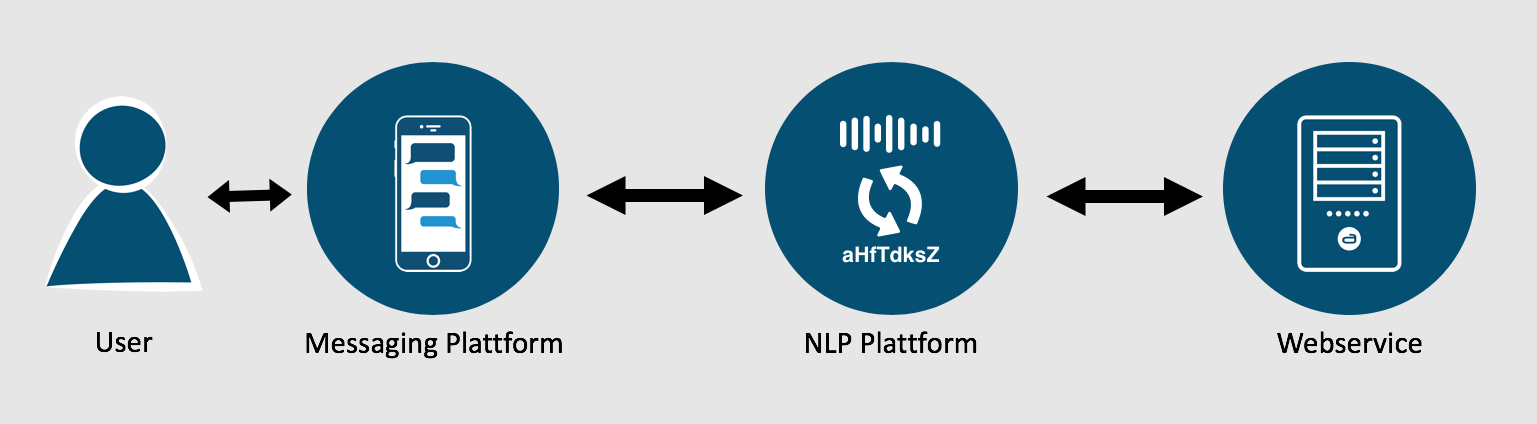
\includegraphics[width=0.9\textwidth]{bilder/Komponenten-v1.png}
    \caption{Übersicht der drei Hauptkomponenten}
    \label{fig:Komponenten-v1}
\end{figure}

\subsection{Frontend}
\label{subsec:frontend}

Zu Beginn jeder Interaktion mit einem Chatbot steht ein Frontend oder, wie in \ref{subsec:cui-chatbot} bezeichnet, eine Messaging Platform. Diese stellt gewissermaßen das Interface dar, über das der User seine Nachrichten eingeben und abschicken kann. 

Wie bereits eingangs erwähnt, gibt es einige Nachrichtenplattformen, in denen Chatbots entwickelt und integriert werden können. Häufig verwendet werden hierbei der Facebook Messenger, WeChat oder Slack. Teilweise bieten diese Plattformen bereits die Möglichkeit zur Darstellung und Integration von \ac{UI}-Elementen in Form von Buttons oder Auswahllisten. Die Vorgehensweise und Umsetzung ist dabei allerdings gleichermaßen einfach wie begrenzt. Während es relativ unkompliziert möglich ist, Antwortmöglichkeiten auf die Frage eines Chatbots via Popup-Buttons zu visualisieren, sind komplexere oder modifizierte \ac{UI}-Elemente nur schwierig bis gar nicht \mbox{umsetzbar}. 

Nachdem die \adorsys \, den Google-Kalender nutzt gibt es von Beginn an den Wunsch bzw. die Idee, dass die Nutzer des Chatbots sich mit dem gewöhnlichen Firmenaccount und der Endung \textit{@adorsys.de} anmelden und authentifizieren können. Die Integration des Firmenkontos in eine andere Nachrichtenplattform erscheint dabei weder besonders sinnvoll noch risikofrei. 

All diese Kriterien führen dazu eine eigene, unabhängige Lösung zu nutzen. Wie bereits dem Titel der Arbeit zu entnehmen ist, handelt es sich dabei um eine Android Applikation. 

\subsection{NLP-Plattform}
\label{subsec:nlp-plattform}

Ein wesentlicher Bestandteil des Chatbots ist die \ac{NLP}-Plattform. Nach der Entscheidung aus \ref{subsec:frontend} sollte dabei nach Möglichkeit ein Android \textit{\ac{SDK}} zur Verfügung stehen. Ein \ac{SDK} ist typischerweise eine Ansammlung von Tools und bereits geschriebenem Programmcode, die bei der Entwicklung von Software-Anwendungen unterstützen. Wichtig ist zudem, dass an die Plattform ein \textit{Server} angebunden werden kann. Die Applikation soll zunächst auf \textit{Deutsch}, später möglicherweise auch noch auf \textit{Englisch} umgesetzt werden. Daher werden auch die beiden zu unterstützenden Sprachen \mbox{betrachtet}. 

Nachdem der Chatbot eine Raumreservierung durchführen soll, muss die ausgewählte \ac{NLP}-Plattform entsprechende Systementitäten unterstützen und erkennen. Wichtig sind in diesem Zusammenhang vor allem Entitäten für \textit{Datum}, \textit{Uhrzeit}, \textit{Dauer} und \textit{Anzahl}. Während sich \textit{Datum}, \textit{Uhrzeit} und \textit{Dauer} auf die Start- und Endzeit des Termins beziehen, können durch die Entität \textit{Anzahl} Informationen über die Anzahl der teilnehmenden Personen gewonnen werden. Zudem wird eine möglichst unbeschränkte und kostenfreie \textit{Nutzung} in Bezug auf die Anzahl der Anfragen (engl. \textit{queries}) \mbox{betrachtet}. 

Auf Basis dieser Anforderungen werden im Folgenden einige der bekanntesten Plattformen für \textit{\acl{NLP}} miteinander verglichen. Nach \cite{riya_study_2018} sind dies derzeit die Plattformen \textit{Dialogflow} von Google, \textit{Wit.ai} von Facebook, Amazon \textit{Lex}, Microsoft \textit{Luis} und IBM \textit{Watson}. 
\newline

\begin{table}[!htb]
\centering
 \begin{tabular}{ | C{3cm} || C{1.8cm}| C{1.8cm} | C{1.8cm} | C{1.8cm} | C{1.8cm} |} 
 \hline
  & Dialogflow & Wit.ai & Lex & Luis & Watson \\
 \hhline{=::=====}
 Android \ac{SDK} & \cmark & \xmark & \cmark & \cmark & \danger \\
 \hline Serveranbindung & \cmark & \cmark & \cmark & \cmark & \cmark \\ 
 \hline Sprache: Deutsch & \cmark & \cmark & \xmark & \cmark & \xmark \\ 
 \hline Sprache: Englisch & \cmark & \cmark & \cmark & \cmark & \cmark \\ 
 \hline Entität: Datum & \cmark & \cmark & \cmark & \cmark & \cmark \\
 \hline Entität: Uhrzeit & \cmark & \cmark & \cmark & \cmark & \cmark \\
 \hline Entität: Dauer & \cmark & \cmark & \xmark & \cmark & \cmark \\
 \hline Entität: Anzahl & \cmark & \cmark & \cmark & \cmark & \cmark \\ 
 \hline Freie Nutzung & \cmark & \cmark & \danger & \danger & \danger \\
 \hline
\end{tabular}
\caption{Vergleich verschiedener NLP-Plattformen}
\label{tab:nlp-plattform-vergleich}
\end{table}

Die Informationen aus Tabelle \ref{tab:nlp-plattform-vergleich} stützen sich auf die Inhalte in \cite{cabot_technology_solution_analysis_2018}, \cite{wit_wit_2018} und \cite{amazon_lex_built-slot_2018}. Erfüllte Anforderungen sind mit einem \textit{grünen Haken} und nicht erfüllte mit einem \textit{roten Kreuz} versehen. Die \textit{gelben Warndreiecke} bedeuten, dass die Anforderungen nur teilweise oder unter bestimmten Bedingungen erfüllt werden. Im Fall von IBM Watson gibt es beispielsweise kein offizielles \textit{Android \ac{SDK}}, es unterstützt allerdings die Programmiersprache Java. Im Zusammenhang mit der Anforderungen \textit{Freie Nutzung} bedeutet ein gelbes Dreieck, dass die Plattform nur einen bestimmten Zeitraum oder bis zu einer bestimmten Anzahl an Anfragen kostenfrei ist. 

Aufgrund der Erkenntnisse aus Tabelle \ref{tab:nlp-plattform-vergleich} fällt die Wahl auf die Plattform Dialogflow. Diese erfüllt alle Anforderungen und kann ohne zusätzliche Kosten genutzt werden. 

\subsection{Webservice}
\label{subsec:webservice}

In Anlehnung an den Abschnitt \ref{subsec:cui-chatbot} wird bei der Umsetzung eines intelligenten Chatbots, der mehr als nur \textit{short answers} gibt, immer ein Backend für das \acl{DM} genutzt. Der Server muss also die von der \ac{NLP}-Plattform Dialogflow bereitgestellten \ac{JSON}-Objekte verarbeiten. In diesem Fall kommen auf den Webservice weitere Aufgaben in Form von Authentifizierung, Kalenderfreigabe oder die Abfrage von freien Räumen zu. 

Bei der Implementierung des Backends wird \textit{Node.js} verwendet. Node.js ist eine serverseitige \textit{\ac{JS}} Plattform und zudem kompatibel zu Dialogflow. Mit Hilfe von Node.js lässt sich ein Webserver realisieren. Zusätzlich lassen sich vorkompilierte Module oder einfache JavaScript-Dateien einbinden. Die Verwaltung der Module übernimmt der \textit{\ac{npm}}. Dieser hilft bei der Installation und Aktualisierung der Module und berücksichtigt dabei auch deren Abhängigkeiten untereinander. Der \ac{npm} macht es somit einfach, den Webserver mit beliebigen Modulen zu erweitern.

Der Server muss also Zugriff auf weitere Daten, Module und \acp{API} haben, welche im Folgenden kurz beschrieben werden. 

\begin{itemize}
\item Zur Verwaltung von Terminen kann die Schnittstelle \textbf{\textit{Goolge Calendar \ac{API}}} verwendet werden. Damit können unter anderem Termine für einen Nutzer erstellt, geändert oder gelesen werden. 
\item An die Datenbank bestehen in diesem Status noch keine speziellen Anforderungen. Es sollen gegebenenfalls Einträge der User mit Profilinformationen und Zugriffstoken für die Kalender-Authentifizierung abgespeichert werden. Dazu reicht ein einfaches \textit{\ac{NoSQL}}-Datenbank\-system wie \textbf{\textit{MongoDB}}. 
\item Zudem müssen die im Office verfügbaren Büroräume nach ihrer Verfügbarkeit abgefragt und an das Backend angebunden werden. Die Besprechungsräume sind dabei als Ressourcen in der Domäne der \adorsys\ angelegt und können ebenfalls über die Google Calendar \ac{API} angesprochen werden.
\end{itemize}

Eine Übersicht aller Komponenten ohne Kommunikation zeigt die Abbildung \ref{fig:komponenten-v2}.
\newline

\begin{figure}[H]
    \centering
    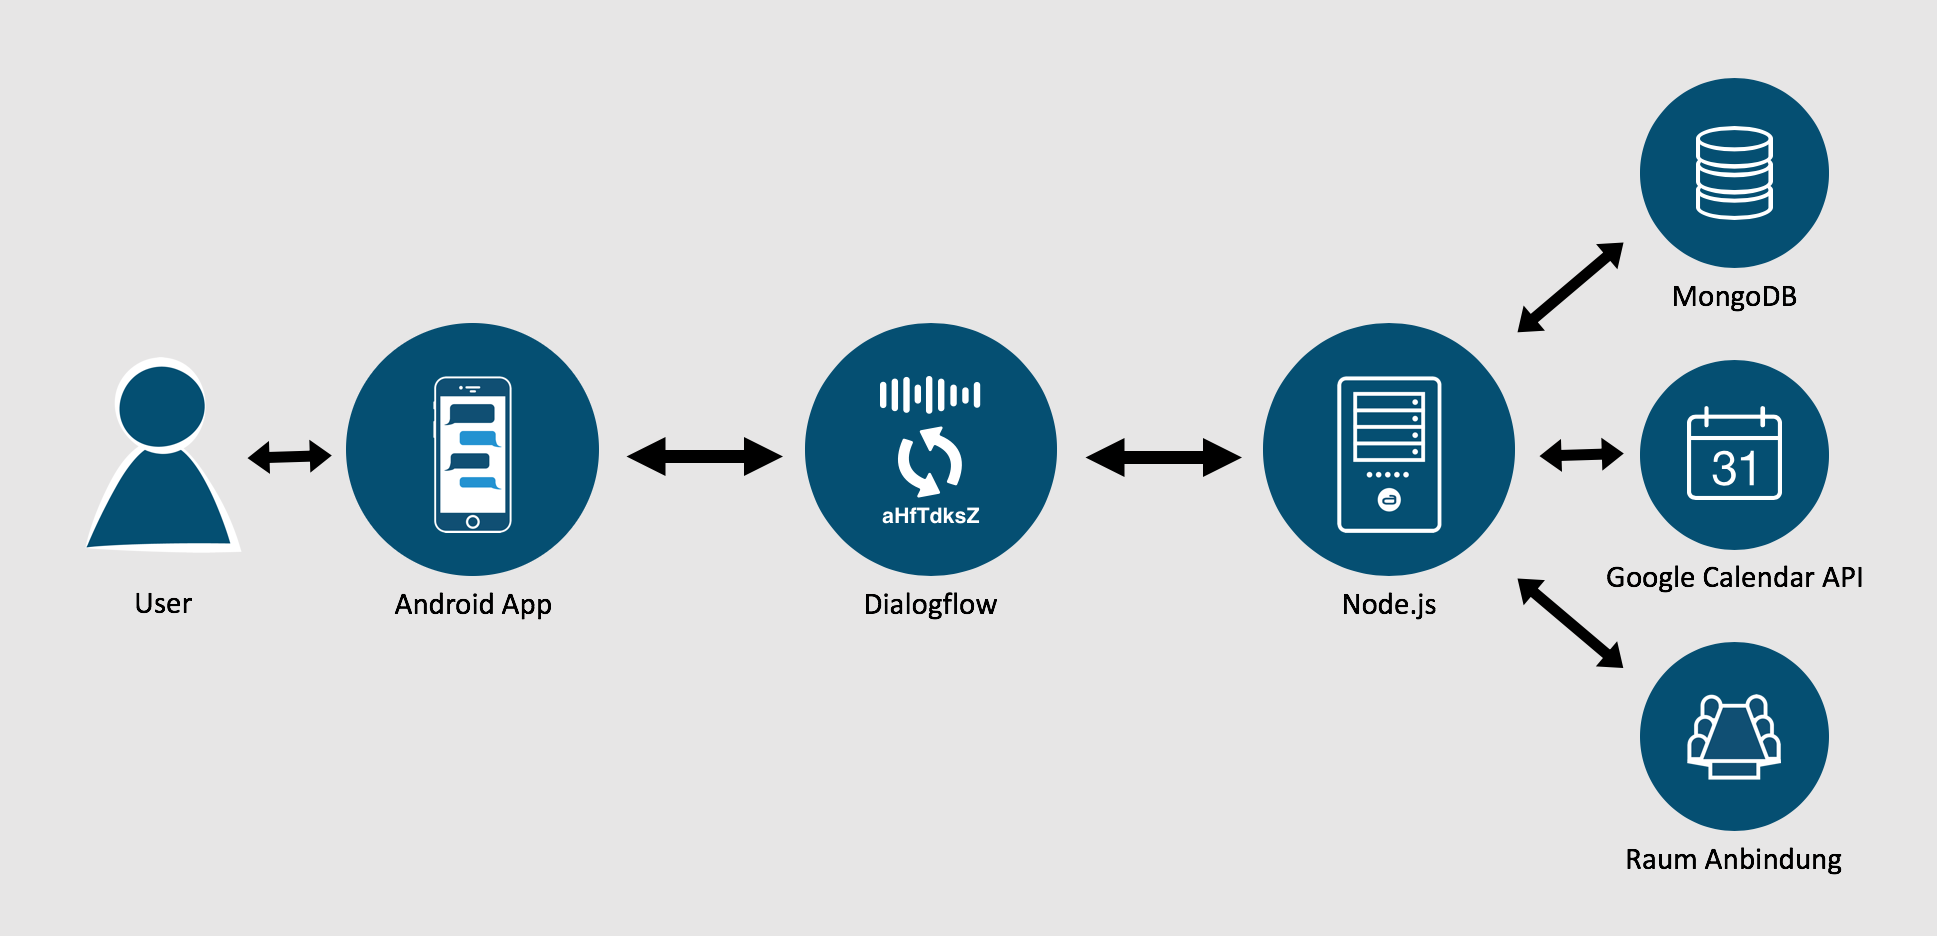
\includegraphics[width=1\textwidth]{bilder/Komponenten-v2.png}
    \caption{Übersicht aller Komponenten ohne Kommunikation}
    \label{fig:komponenten-v2}
\end{figure}

\section{Kommunikation}
\label{sec:kommunikation}

Nachdem im vorangegangenen Kapitel \ref{sec:auswahl-komponenten} die verschiedenen Komponenten beschrieben wurden, stellt sich nun die Frage wie all diese unterschiedlichen Plattformen miteinander kommunizieren. Um dies zu beantworten, werden einige in der Arbeit erprobten Ansätze erläutert und bewertet. 

\subsection{Authentifizierung und Autorisierung}
\label{subsec:authentifizierung-authorisierung}

Wie bereits eingangs erwähnt, nutzt die \adorsys\ den Google-Kalender. Für den Nutzer ist es demnach wünschenswert und komfortabel, wenn er sich in der App auf einer Art \textit{Loginpage} anmelden kann. Genutzt werden können dazu die gewöhnliche E-Mail-Adresse mit der \textit{@adorsys.de}-Endung, welche auf dem Google-Kalender basiert, und das entsprechende Passwort. Der Login innerhalb der App kann für beliebige Anwendungszwecke konfiguriert werden. So lassen sich dabei in der Basisvariante nach erfolgreicher Anmeldung beispielsweise Profilinformationen wie Vor- und Nachname oder der individuelle \ac{ID} eines Nutzers (auch \textit{Person-\ac{ID}}) gewinnen. Je nach Anwendungsfall kann zudem die E-Mail-Adresse oder auch ein \textit{Android-\ac{ID}-Token} erhalten werden. Zu dem Android-\ac{ID}-Token können zusätzlich so genannte \textit{Scopes} hinzugefügt werden, die beispielsweise Lese- oder Schreibzugriff auf den Kalender gewähren. \cite{google_developers_integrating_2018} 

Die erste Idee ist hierbei, bei Anmeldung in der App einen Android-\ac{ID}-Token zu erhalten, der durch alle Komponenten durchgeschleift wird. Dieser würde also über die Textanbindung der App an Dialogflow und deren Verarbeitung im Backend mitgeliefert werden. Damit wäre in jedem Schritt klar, von wem die aktuelle Textnachricht kommt. Außerdem kann jederzeit auf Profilinformationen zugegriffen werden. Bei genauerer Betrachtung treten hierbei zwei wesentliche Probleme auf. Zum einen gibt es keine Möglichkeit, über das Android \ac{SDK} weitere Daten in die Textanfrage an Dialogflow zu stecken. Das \ac{JSON}-File wird anhand des eingegebenen Textes und weiterer Konfigurationen automatisch erzeugt und kann somit nicht modifiziert werden. Ein weiteres Problem stellt sich bei der Authentifizierung mittels Android-\ac{ID}-Token im Backend dar. Aus Sicherheitsgründen ist es nicht möglich, mit einem Token aus einer Android Applikation im Backend auf Kalenderereignisse zuzugreifen \cite{google_developers_authenticate_2018}. 

Für den Zugriff auf Kalenderereignisse im Backend ist nämlich ein eigener, serverseitiger \textit{access token} notwendig. Dieser kann nach dem Aufruf eines Authentifizierungslinks und der Generierung eines Authentifizierungscodes schließlich im Backend erzeugt werden. Mitgeliefert wird dabei noch ein dazugehöriger \textit{refresh token}, der bei Ablauf zur Generierung eines neuen \textit{access token} genutzt werden kann. Außerdem gibt es die Möglichkeit der Verifizierung des Android-\ac{ID}-Tokens im Backend. Über entsprechende Bibliotheken und Methoden kann dabei der Android-\ac{ID}-Token verfiziert und Basis-Profilinformationen wie Name, E-Mail-Adresse oder Person-\ac{ID} herausgefunden werden. 

Zunächst wird noch ein weiterer Ansatz verfolgt. Dabei muss überlegt werden, woran eine Nachricht von bzw. an Dialogflow identifiziert werden kann. Im \ac{JSON}-File von Dialogflow steht neben den Informationen zum geschriebenen Text, dem Intent und verschiedenen Entitäten auch eine \ac{ID} für die aktuelle Session. Diese \textit{Session-\ac{ID}} bleibt dabei im Laufe einer Konversation unverändert und kann somit als \acl{ID} im Backend verwendet werden. Um im Backend zu wissen, zu wem diese Session-\ac{ID} gehört, muss ihr ein weiterer \acl{ID} zugeordnet werden. Denkbar wäre hierbei eine universelle \textit{Device-\ac{ID}} des Geräts. Es gibt dazu mehrere Möglichkeiten, wie beispielsweise eine sogenannte \textit{Unique Telephony Number}, die \textit{MAC-Adresse}, eine \textit{Seriennummer} oder eine \textit{Secure Android-\ac{ID}} \cite{saurel_s._how_2018}. 

Eine dieser Device-\acp{ID} würde dann zusammen mit der Session-\ac{ID} in einer Datenbank liegen, wo sie als gemeinsamer Eintrag miteinander verknüpft werden. Verarbeitet der Server nun im Rahmen des \aclp{DM} eine Nutzeranfrage, kann anhand der Session-\ac{ID} die dazugehörige Device-\ac{ID} aus der Datenbank geholt und somit die Anfrage einem konkreten Nutzer bzw. Gerät zugeordnet werden. Außerdem können zu diesen Einträgen passende Token für den Zugriff auf den Google-Kalender in der Datenbank hinterlegt werden. 

Nachteilig an der Lösung mit der Verknüpfung von Session-\ac{ID} und Device-\ac{ID} ist, dass diese beiden Werte keinerlei Informationen über die Identität des Nutzers geben. Hier kann nun wieder der Google-Login innerhalb der App genutzt werden. Nachdem der User sich erfolgreich angemeldet hat, stehen seine persönlichen Informationen wie Name, E-Mail-Adresse und Person-\ac{ID} zur Verfügung. Nachdem die Person-\ac{ID} universell und für jedes Google-Konto eindeutig ist, kann diese problemlos für den Datenbankeintrag und die damit verbundene Verknüpfung zur Session-\ac{ID} und den Token aus dem Backend verwendet werden. Die Device-\ac{ID} wird damit überflüssig. Im Backend kann die Session-\ac{ID} dann jederzeit über die Abfrage einer Datenbank zugeordnet und entsprechende Daten für die Identität des Users oder seine Token für den Kalenderzugriff gelesen werden. 

Nach ausführlicher Betrachtung stellt sich die Möglichkeit einer Zuordnung des Users durch seine aktuelle Session-\ac{ID} und der Person-\ac{ID} seines Google-Accounts als beste Möglichkeit heraus. Wird der Google-Login innerhalb einer App genutzt, um sich im Backend zu authentifizieren, sollten die Informationen in jedem Fall verschlüsselt übertragen werden \cite{google_developers_authenticate_2018}. Dazu kann der innerhalb der Android App generierte \ac{ID}-Token an den Server gesendet und dort authentifiziert werden. Anschließend können daraus alle notwendigen Profilinformationen exportiert und in einer Datenbank zusammen mit der entsprechenden Session-\ac{ID} gespeichert werden. Möchte der User auf seinen Kalender zugreifen, muss er dies innerhalb der App einmalig mittels einer im Backend generierten \ac{URL} bestätigen. Anschließend werden sein \textit{access token} und \textit{refresh token} in der Datenbank hinterlegt. Aus den vorhergehenden Überlegungen ergibt sich für die Struktur zur Kommunikation zwischen den Komponenten das Schaubild aus Abbildung \ref{fig:komponenten-v3}.
\newline

\begin{figure}[htb]
    \centering
    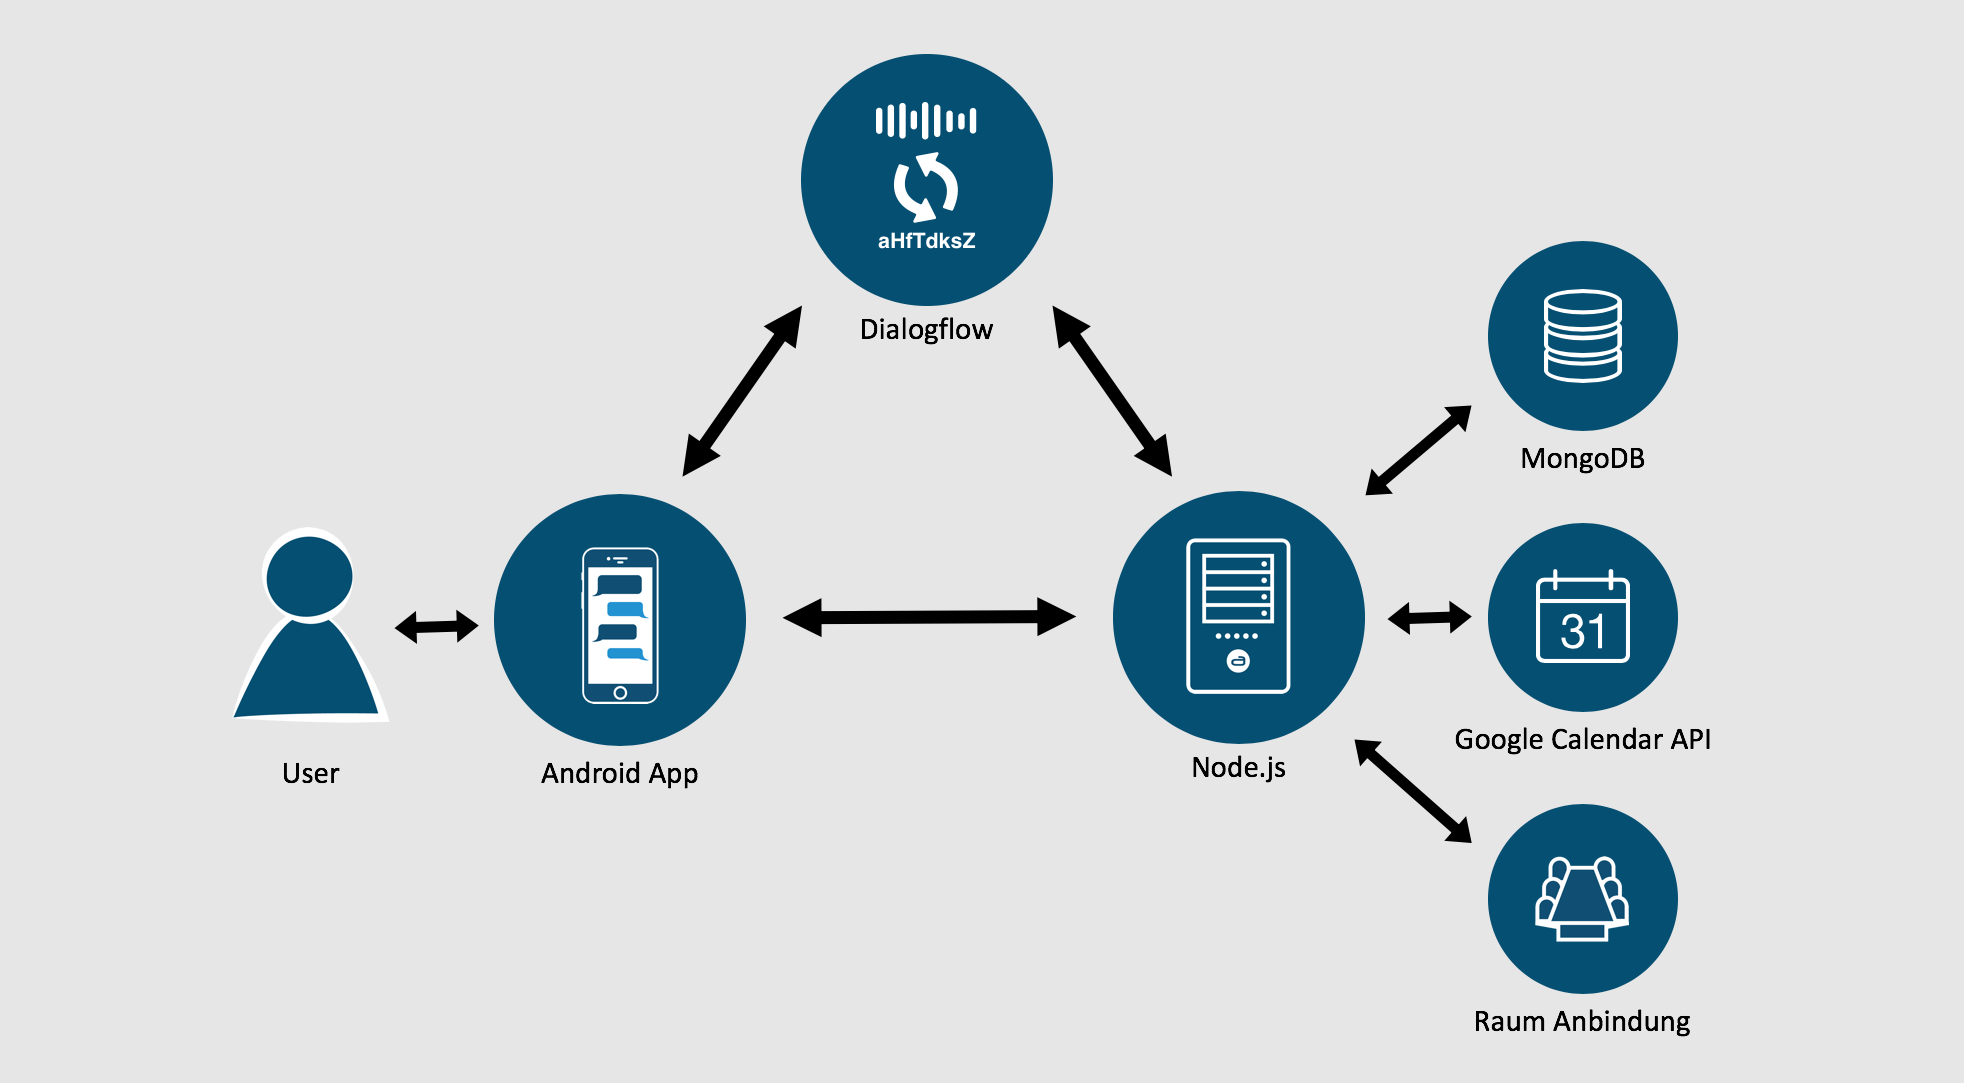
\includegraphics[width=1\textwidth]{bilder/Komponenten-v3.png}
    \caption{Übersicht aller Komponenten mit Kommunikation}
    \label{fig:komponenten-v3}
\end{figure}

\subsection{Schnittstellen}
\label{subsec:Schnittstellen-Konzeption}

Als Schnittstellen zwischen den Komponenten kommen verschiedene Techniken zum Einsatz. Die verwendeten Techniken sollen daher im Folgenden kurz erläutert \mbox{werden}. 

\begin{enumerate}
  \item Von einer Android Applikation aus kann das \textit{Android \ac{SDK} für api.ai}\footnote{api.ai heißt jetzt Dialogflow} genutzt werden, um Anfragen an Dialogflow zu senden \cite{skachkov_dialogflow-android-client:_2018}. Damit können sowohl sprach- als auch textbasierte Anfragen an Dialogflow gesendet und die Antworten ausgewertet werden. 
  
  \item Zur Kommunikation zwischen der Android App und dem Node.js Webservice kann \textit{Retrofit} verwendet werden. Retrofit ist ein \ac{REST} Client für Android und Java und basiert auf der \textit{OkHttp} Bibliothek. Damit ist es möglich, strukturierte Daten (z.B. \ac{JSON}) zu einem \ac{REST}-basierten Webservice zu schicken oder abzurufen. \cite{vogel_using_2018} 
  
  \item Mit Hilfe von \textit{Bespoken} kann eine Verbindung vom Dialogflow Agent auf den lokalen Rechner hergestellt werden. Über einen Proxy-Dienst gibt das Tool eine \ac{URL} aus, welche im Agent als Webhook hinterlegt wird \cite{bespoken_api.ai_2018}. Dies ist allerdings nur so lange relevant, wie der Webservice auf einem lokalen Rechner läuft. Zum einem späteren Zeitpunkt kann hier auf eine \ac{REST}-Schnittstelle zurückgegriffen werden. 
  
  \item Um vom Node.js Webserver aus mit einer MongoDB kommunizieren zu können, kann über \ac{npm} ein \textit{MongoDB Driver} installiert werden. Anschließend kann das entsprechende Modul in den Server eingebunden und über eine \ac{API} darauf zugegriffen werden. \cite{npmjs_mongodb_2018}
  
  \item Der Webservice kann Kalenderereignisse über die \textit{Google Calendar \ac{API}} abfragen oder erstellen. Auch diese wird über ein Modul in Node.js eingebunden. Die Google Calendar \ac{API} basiert wiederum auf \ac{REST} und \ac{HTTP}. \cite{google_developers_node.js_2018}
  
  \item Die Raumanbindung im Backend geschieht ebenfalls über die \textit{Google Calendar \ac{API}}. Die Besprechungsräume sind dabei als Ressourcen in der Domäne der \mbox{\adorsys} angelegt und können nach ihrer Verfügbarkeit abgefragt werden.
  
\end{enumerate}

\clearpage
\section{Android Applikation}
\label{sec:android-applikation}

Wie bereits dem Titel der Arbeit zu entnehmen ist und unter \ref{subsec:frontend} nochmals ausführlich erläutert wird, handelt es sich bei dem Frontend bzw. der Messaging Platform des Systems um eine Android App. Über diese Applikation ist es dem Nutzer möglich, sich im Rahmen des Raumbuchungssystems einzuloggen und anschließend durch die Benutzung eines Chatbots Räume zu reservieren. Im Folgenden soll hierzu ein Überblick gegeben, allerdings nicht detaillierter auf den Quelltext eingegangen werden. Es wird dabei versucht, die Bedienung und den Workflow der App beispielhaft zu verdeutlichen. Dabei ist es leider nicht immer möglich, jeden Arbeitsschritt auf seine kleinste Ebene zu zerlegen. Vielmehr werden die prinzipiellen Abläufe anhand einiger Abbildungen erläutert.

\subsection{Manifest}
\label{subsec:manifest}

Im Android Manifest werden einige grundlegende Informationen deklariert. Nachdem die App über Dialogflow mit dem Internet verbunden sein muss, wird eine entsprechende \textit{Permission} im Manifest verwaltet. Des Weiteren werden hier die beiden Aktivitäten \textit{LoginActivity} und \textit{ChatActivity} eingetragen, wobei die LoginActivity als \textit{Main-} bzw. \textit{Launcher-}Aktivität festgelegt und beim Start der App als erstes aufgerufen wird. Zudem kann hier das Icon der Applikation geändert werden. Das Icon wird vom Nutzer angewählt, wenn er die App auf seinem Smartphone starten möchte und hat eine dementsprechend wichtige Bedeutung. Das Icon\footnote{Das Icon wurde von Mona Kögel entworfen} ist in Abbildung \ref{fig:android-app-icon} dargestellt.
\newline

\begin{figure}[H]
    \centering
    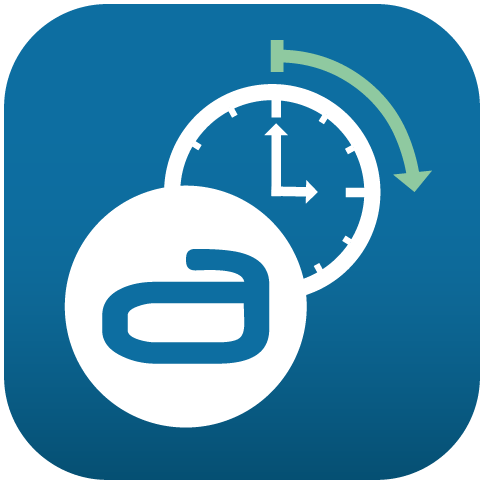
\includegraphics[width=0.2\textwidth]{bilder/AppIcon.png}
    \caption{Icon der Android Applikation}
    \label{fig:android-app-icon}
\end{figure}

\subsection{Anmelden}
\label{subsec:login-activity}

Nach erstmaligem Start der Applikation findet sich der Nutzer auf einer \textit{Loginpage} wieder. Der Login wurde gemäß der offiziellen Dokumentation zum \textit{Google Sign-In für Android Applikationen} integriert \cite{google_developers_integrating_2018}. Abbildung \ref{fig:android-login-screen} zeigt die relevanten \mbox{Anmeldebildschirme}. 

Auf der linken Seite ist der Startbildschirm zu sehen. Betätigt der Nutzer den Button \textit{Sign in}, kann er aus seinen mit dem Android-Device verknüpften Google-Accounts wählen oder einen weiteren beliebigen Account verknüpfen. Nach erfolgreicher Anmeldung steht anschließend ein \textit{Android-\ac{ID}-Token} zur Verfügung, der wie bereits unter \ref{subsec:authentifizierung-authorisierung} beschrieben, im Backend verifiziert werden kann. Erwähnenswert ist in diesem Zusammenhang, dass dieser Login mit allen Google-Konten funktioniert, eine tatsächliche Raumbuchung im späteren Verlauf allerdings nur mit Accounts innerhalb der Domäne der \adorsys\ möglich ist. Ist der Nutzer erfolgreich eingeloggt, ändert sich der \textit{Login Status} auf dem Screen und der User wird automatisch zum Chatbot weitergeleitet.
\newline

\begin{figure}[H]
    \centering
    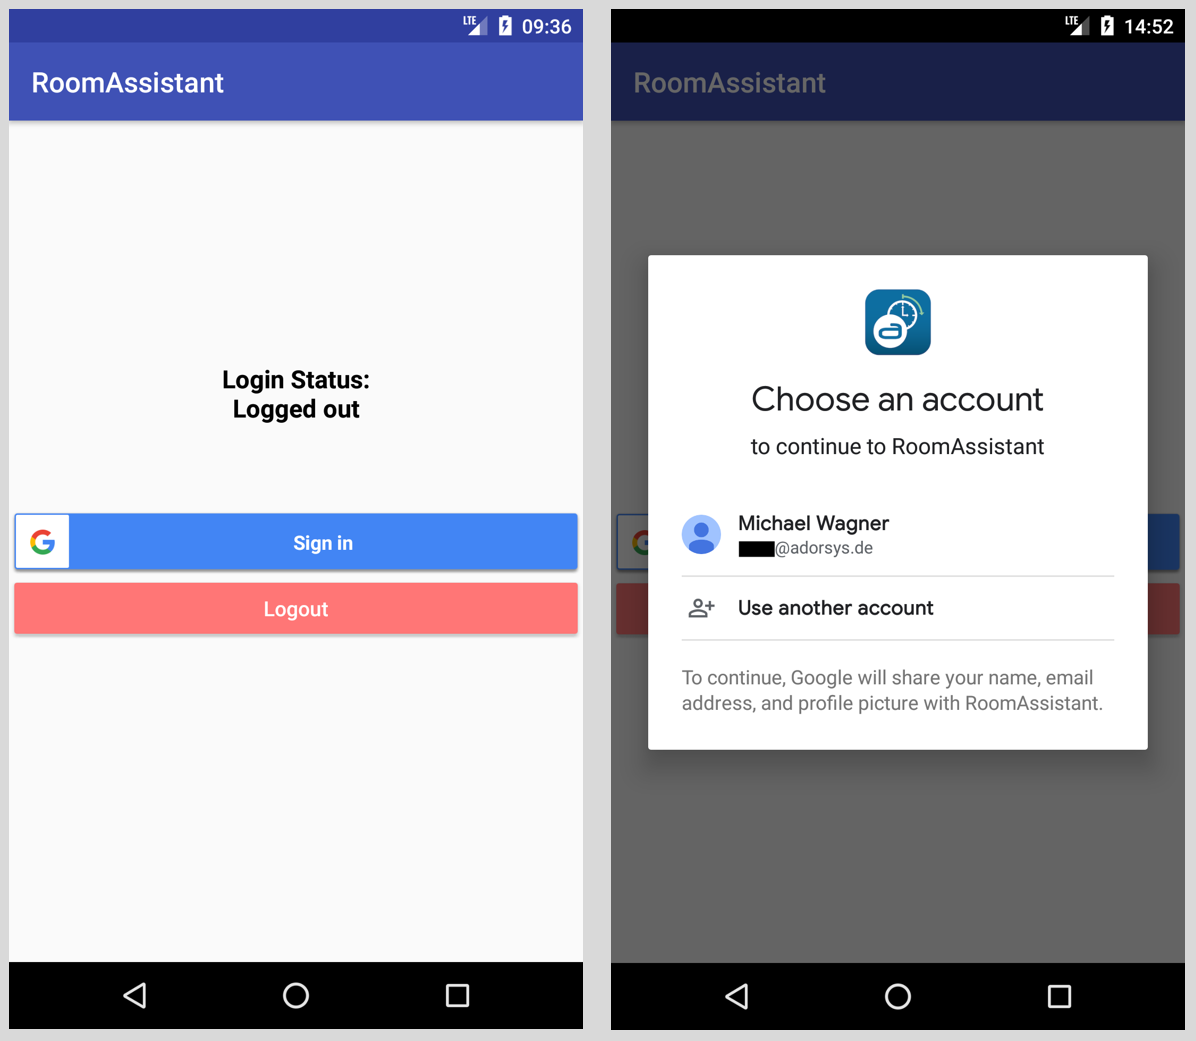
\includegraphics[width=0.8\textwidth]{bilder/LoginScreenCombined.png}
    \caption{Benutzeroberfläche zum Anmelden in der Android Applikation}
    \label{fig:android-login-screen}
\end{figure}

\FloatBarrier
\subsection{Kalenderzugriff}
\label{subsec:authorization-prozess}

Beim Start der \textit{ChatActivity} wird zunächst, vom Nutzer unbemerkt, eine Art \textit{Handshake} durchgeführt. Die Applikation sendet einen Request mit der Query \textit{Hallo} an Dialogflow. Über den Webhook kann diese Anfrage dann im Node.js Webservice ausgewertet werden. Anhand der mitgelieferten Daten können die dazugehörigen Nutzereinträge aus der Datenbank gelesen werden. In diesem Zuge wird auch direkt der Eintrag für die aktuelle Session-\ac{ID} aktualisiert. Anschließend wird geprüft, ob bereits ein gültiger \textit{access token} in der Datenbank vorhanden ist. Eine entsprechende \ac{JSON}-Response wird zunächst zurück an Dialogflow und von dort aus zurück zur Android App gesendet. Abbildung \ref{fig:sequence-diagramm-authorization-flow} verdeutlicht diesen Prozess durch die Darstellung eines entsprechenden Sequenzdiagramms.
\newline

\begin{figure}[H]
    \centering
    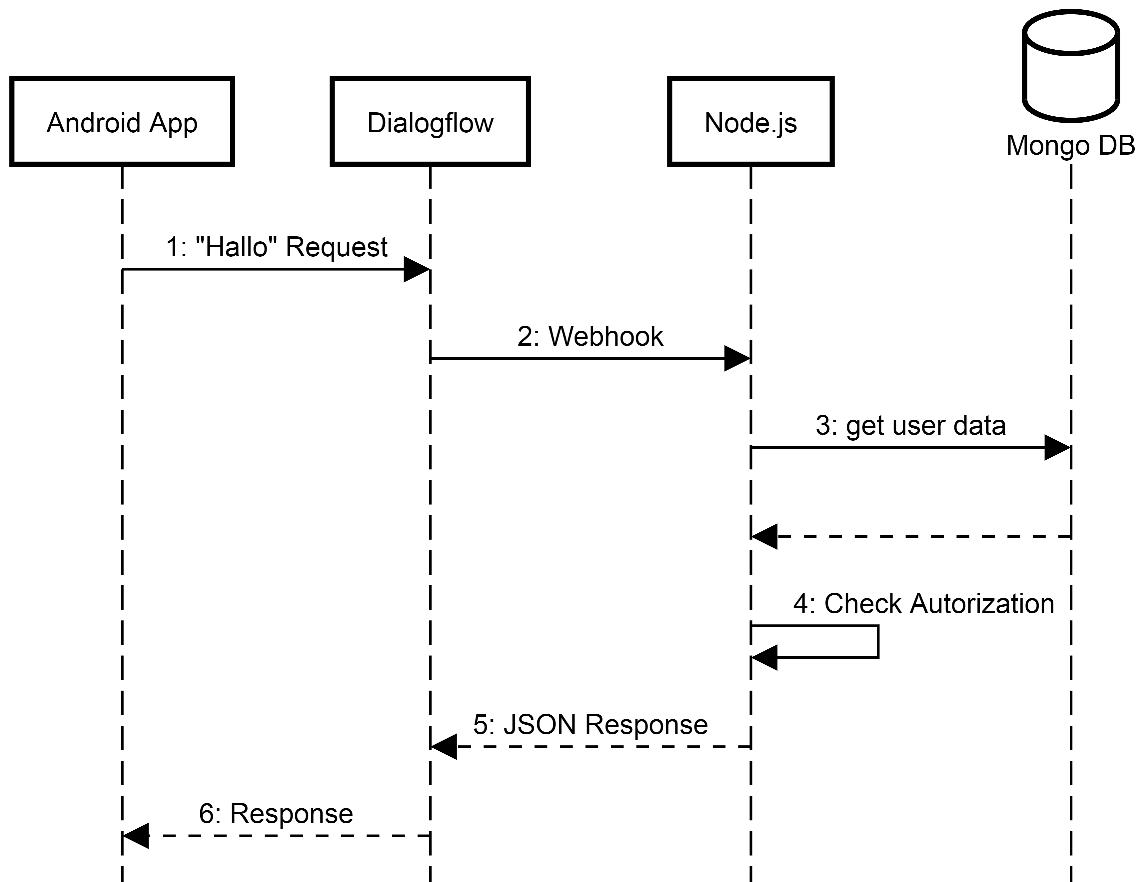
\includegraphics[width=0.9\textwidth]{bilder/Authorization-Flow.png}
    \caption{Sequenzdiagramm zur Autorisierung}
    \label{fig:sequence-diagramm-authorization-flow}
\end{figure}

Ist der User noch nicht autorisiert, wird er durch eine entsprechende Response dazu aufgefordert. Diese Abfolge ist in Abbildung \ref{fig:android-authorization-screen} festgehalten. Innerhalb der \textit{ChatActivity} öffnet sich in diesem Zusammenhang ein Browserfenster (linker Screen), in dem sich der Nutzer anmelden und Zugriff auf seinen Kalender gewähren kann (mittlerer Screen). Hat er dies getan, erhält er einen \textit{Authorization Code}, den er dem Chatbot anschließend zuschickt (rechter Screen). Im Backend wird der entsprechende Code geprüft, der \textit{access token} bzw. \textit{refresh token} generiert und in der Datenbank hinterlegt. Der Chatbot vermeldet dem Nutzer die Nachricht, dass die Autorisierung erfolgreich war. Beim nächsten Konversationsstart kennt der Chatbot den Nutzer und begrüßt ihn mit Phrasen wie \textit{„Hey, willkommen zurück“} oder \textit{„Schön dich zu sehen. Was kann ich für dich tun?“}.
\newline

\begin{figure}[H]
    \centering
    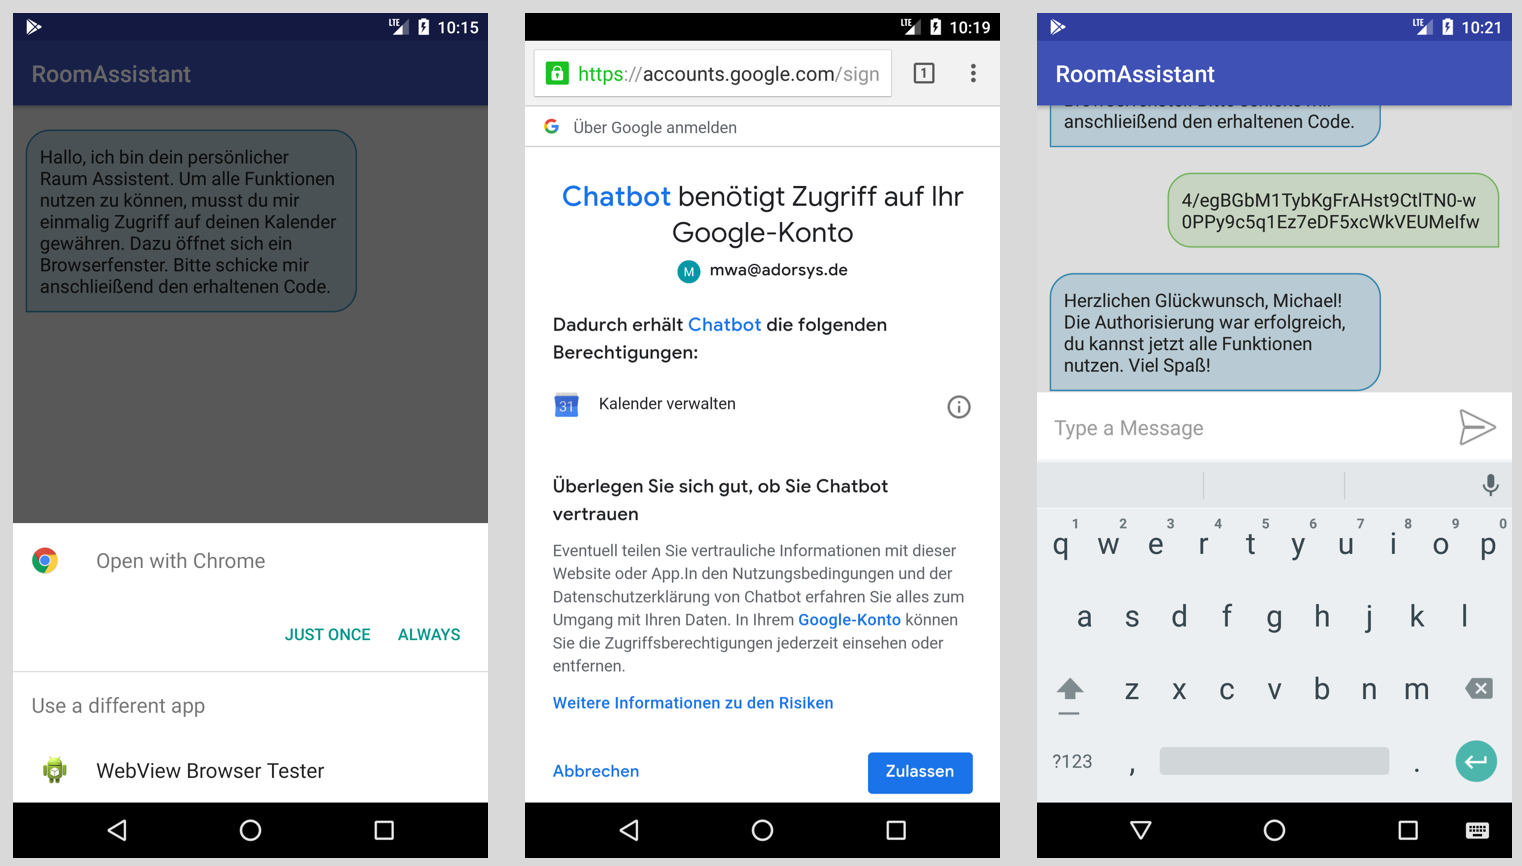
\includegraphics[width=0.9\textwidth]{bilder/AuthorizationScreenCombined.PNG}
    \caption{Benutzeroberfläche zum Autorisieren in der Android Applikation}
    \label{fig:android-authorization-screen}
\end{figure}

\FloatBarrier
\subsection{Chat Interface}
\label{subsec:Chat Interface}

Die \textit{ChatActivity} bzw. das \textit{Chat Interface} stellt das Kernelement der Android Applikation dar. Es besteht im Prinzip aus einer \textit{RecyclerView}, einem \textit{EditText} Feld und einem  \textit{Button}. Diese sind durch mehrere, verschachtelte \textit{RelativeLayouts} so angeordnet, dass sich Eingabefeld und Sendebutton immer am unteren Rand befinden. Bei Eingabe einer Nachricht durch den Nutzer klappt sich eine Tastatur auf und die RecyclerView passt sich entsprechend an. In die RecyclerView können verschiedene Elemente nach und nach eingeschoben werden, sodass für den Nutzer am Ende ein chronologischer und scrollbarer Nachrichtenverlauf sichtbar wird. Dieses Prinzip wurde zuvor bereits im rechten Screen der Abbildung \ref{fig:android-authorization-screen} dargestellt. 

Die \ac{UI}-Erweiterungen sind dabei in einer eigenen \ac{XML}-Datei definiert und werden codeseitig von einer Art \textit{Adapter} verwaltet. Dieser Adapter beinhaltet eine Liste mit Instanzen einer eigenen Klasse \textit{ChatMessage}. Eine Chatmessage hat üblicherweise je ein Attribut für den \textit{Content} und den \textit{Type}. Der Content beschreibt den anzuzeigenden Text, während der Type angibt um welche Art von Nachricht es sich handelt. Aufgrund des Umfangs und der begrenzten Zeit wurden in der Arbeit nur einige im Rahmen der Konzeption entstandenen \ac{UI}-Erweiterungen umgesetzt. Diese werden in Tabelle \ref{tab:arten-nachrichten-chat-interface} genauer erläutert.
\newline

\begin{table}[!htb]
\centering
 \begin{tabular}{ | C{4cm} || C{1.5cm} || C{5cm} || C{2cm} |} 
 \hline
 Type & Art & Beschreibung & Orientierung \\
 \hhline{=::===}
 \hline MSG\_SENT & Text & Textnachricht User & rechts \\ 
 \hline MSG\_RECEIVED & Text & Textnachricht Chatbot & links \\ 
 \hline BUTTON\_YES\_NO & Buttons & Textnachricht mit Buttons ja/nein & links \\ 
 \hline SLIDER\_DURATION & Slider & Textnachricht mit Slider für Dauer & links \\ 
 \hline
\end{tabular}
\caption{Arten von Nachrichten im Chat Interface}
\label{tab:arten-nachrichten-chat-interface}
\end{table}

Diese Unterscheidung macht es möglich, der RecyclerView je nach Ausgangspunkt unterschiedliche \ac{UI}-Elemente hinzuzufügen. Ein beispielhafter Konversationsablauf mit allen implementierten \ac{UI}-Elementen ist in Abbildung \ref{fig:android-chat-interface-screen} dargestellt. 

Sendet der User eine Textnachricht an den Chatbot, erscheint seine rechtsbündige Textnachricht mit entsprechender farblicher Kennzeichnung. Entsprechendes gilt analog für die Textnachrichten des Chatbots. Auch das Feature \textit{Chatbot is thinking} kann somit implementiert werden. Dazu wird nach Abschicken der Nutzeranfrage an Dialogflow eine Textnachricht vom Typ \textit{MSG\_RECEIVED} in die RecyclerView geschoben. Diese bleibt dort so lange, bis die Antwort vom Backend und über Dialogflow zurück kommt. 

Dies dauert je nach Komplexität in der Regel wenige Sekunden. Der Nutzer erhält also direkt Feedback, dass seine Anfrage bearbeitet wird. Wurde die Response erhalten, kann das Element wieder entfernt werden und je nach Nachrichtenart die tatsächliche Rückmeldung des Systems angezeigt werden. Slider oder Buttons lassen sich nun wie gewohnt bedienen. Wird eine Auswahl über einen Button bestätigt, senden die \textit{onClick} Ereignisse eine Nachricht in textueller Form an Dialogflow und der Ablauf beginnt wieder von vorne. 

Da alle Eingaben des Nutzers über Dialogflow laufen und dort in Form einer \mbox{Textquery} ankommen müssen, lässt sich das System auch jederzeit über das Texteingabefeld bedienen. Die \ac{UI}-Erweiterungen dienen lediglich als Vorschlag und Angebot durch das System und sollen gegebenenfalls die Bedienung des Chatbots erleichtern.
\newline

\begin{figure}[H]
    \centering
    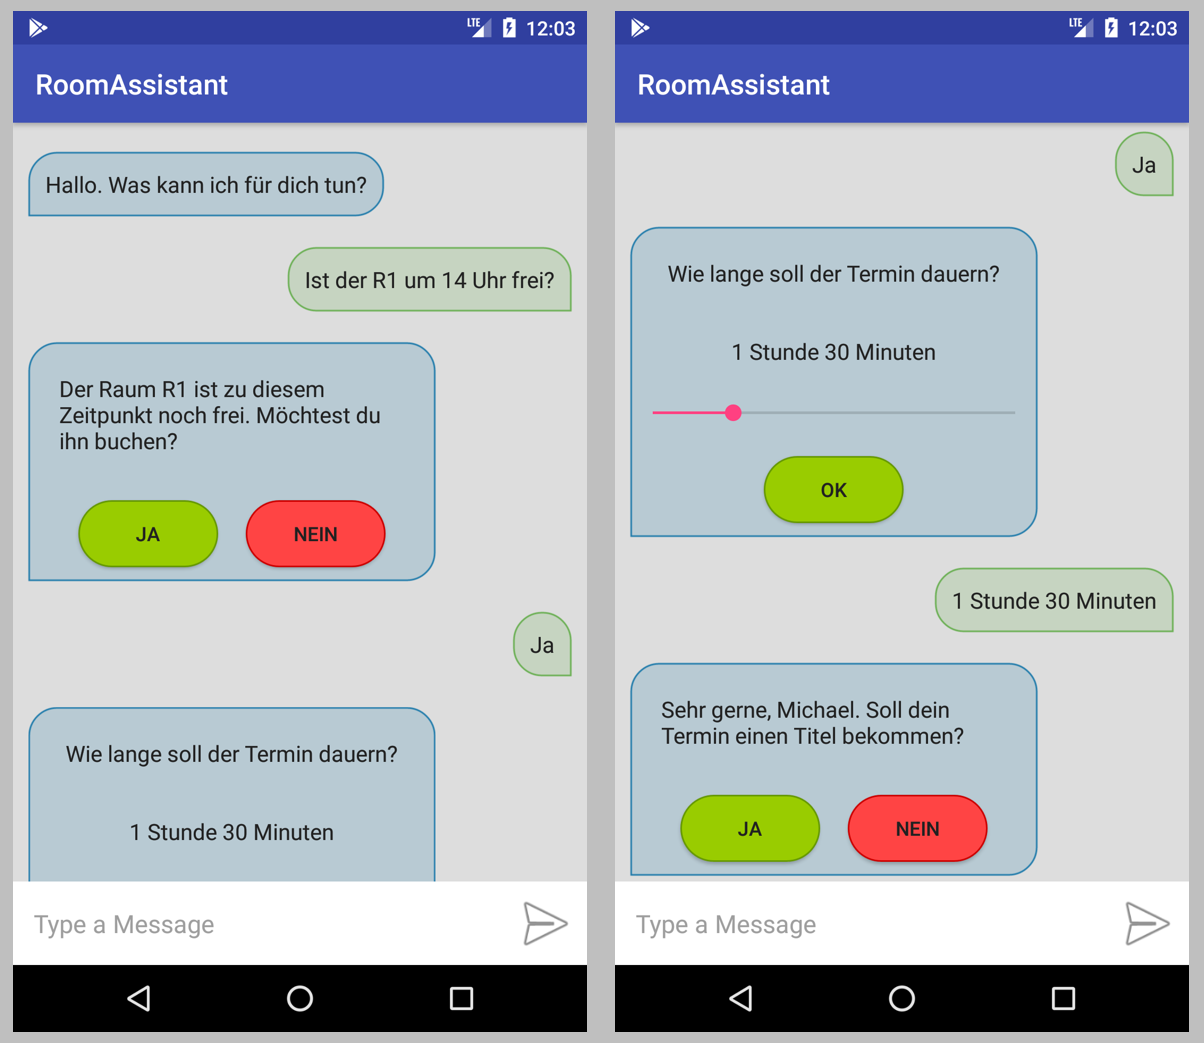
\includegraphics[width=0.9\textwidth]{bilder/ChatInterfaceCombined.png}
    \caption{Chat Interface in der Android Applikation}
    \label{fig:android-chat-interface-screen}
\end{figure}

Es ist nicht immer leicht, das Prinzip und den Umgang mit einer mobilen Applikation nur durch textuelle Beschreibung und Abbildungen darzustellen. Um die Bedienung und den Workflow der Android Applikation greifbarer zu machen, befinden sich auf der CD im Anhang einige \textit{Videos} zum beispielhaften Ablauf einer \textit{Autorisierung}, \textit{Raumbuchung} oder \textit{-abfrage}.



\clearpage
\section{Dialogflow Agent}
\label{sec:dialogflow-agent}

Nach dem ausführlichen Vergleich verschiedener \ac{NLP}-Plattformen in  \ref{subsec:nlp-plattform} fiel die Wahl auf Dialogflow. Die prinzipielle Aufgabe der \ac{NLP}-Plattform ist es, die Intents und Entitäten der Nutzeranfrage zu erkennen und richtig zuzuordnen. Außerdem ist Dialogflow für einen möglichst flüssigen Konversationsflow zuständig. All diese Aufgaben kombiniert in diesem Zusammenhang ein so genannter \textit{Agent}. 

Abbildung \ref{fig:dialogflow-agent-overview} zeigt den prinzipiellen Aufbau eines \textit{Dialogflow Agents} (orange Komponenten). Im Grunde kann dieses Strukturbild analog zu der Abbildung \ref{fig:komponenten-v2} betrachtet werden. 
\newline

\begin{figure}[H]
    \centering
    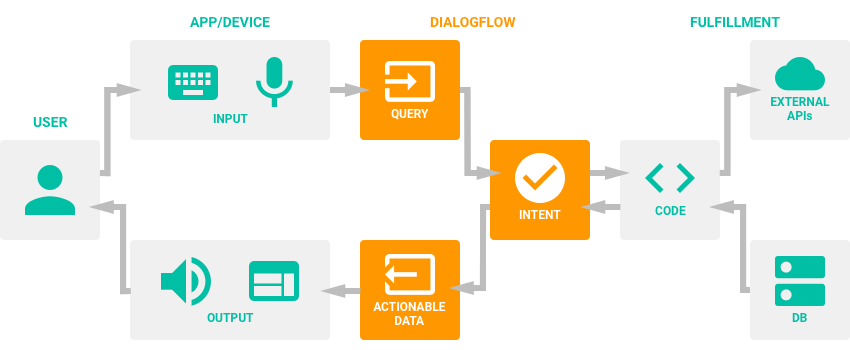
\includegraphics[width=0.9\textwidth]{bilder/dialogflow-agent.png}
    \caption{Prinzipieller Aufbau eines Dialogflow Agents \cite{google_cloud_agents_2018}}
    \label{fig:dialogflow-agent-overview}
\end{figure}

Die linke Seite stellt den User inklusive seiner Ein- und Ausgabemöglichkeiten dar. Im Rahmen der Arbeit ist dies die zuvor beschriebene Android Applikation. Direkt danach ist der Dialogflow Agent anzuordnen. Er erhält eine Query, also die Nutzeranfrage in Textform, ordnet diese einem Intent zu und zieht die relevanten Entitäten heraus. Das hier als \textit{Fulfillment} bezeichnete stellt im Rahmen der Arbeit das Backend dar. Hier werden die Intents und Entitäten ausgewertet und externe \acp{API} oder Datenbanken angebunden. Eine entsprechende Response gelangt dann auf dem Rückweg wiederum über Dialogflow an den User. 

\subsection{Intents}
\label{subsec:agent-intents}

Aufgrund der begrenzten Zeit liegt der Fokus in der Implementierung auf der grundlegenden Funktion. Dazu soll es möglich sein, über das \acl{CUI} nach freien Räumen zu suchen und diese zu reservieren. Auch die Umsetzung der Intents wird daher auf diese beiden Fälle beschränkt. Zudem gibt es standardmäßig bei der Erstellung eines \textit{Agents} je einen \textit{Default Welcome Intent} zur Begrüßung und einen \textit{Default Fallback Intent} als Absicherung, wenn der Chatbot den Nutzer nicht verstanden hat. Um die verschiedenen Intents und Abläufe etwas konkreter darstellen zu können, sind diese in Abbildung \ref{fig:dialogflow-agent-structure} zusammengefasst. Die Abbildung dient der Verdeutlichung des Workflows und stimmt daher nicht eins zu eins mit dem tatsächlichen Agent überein. 
\newline

\begin{figure}[H]
    \centering
    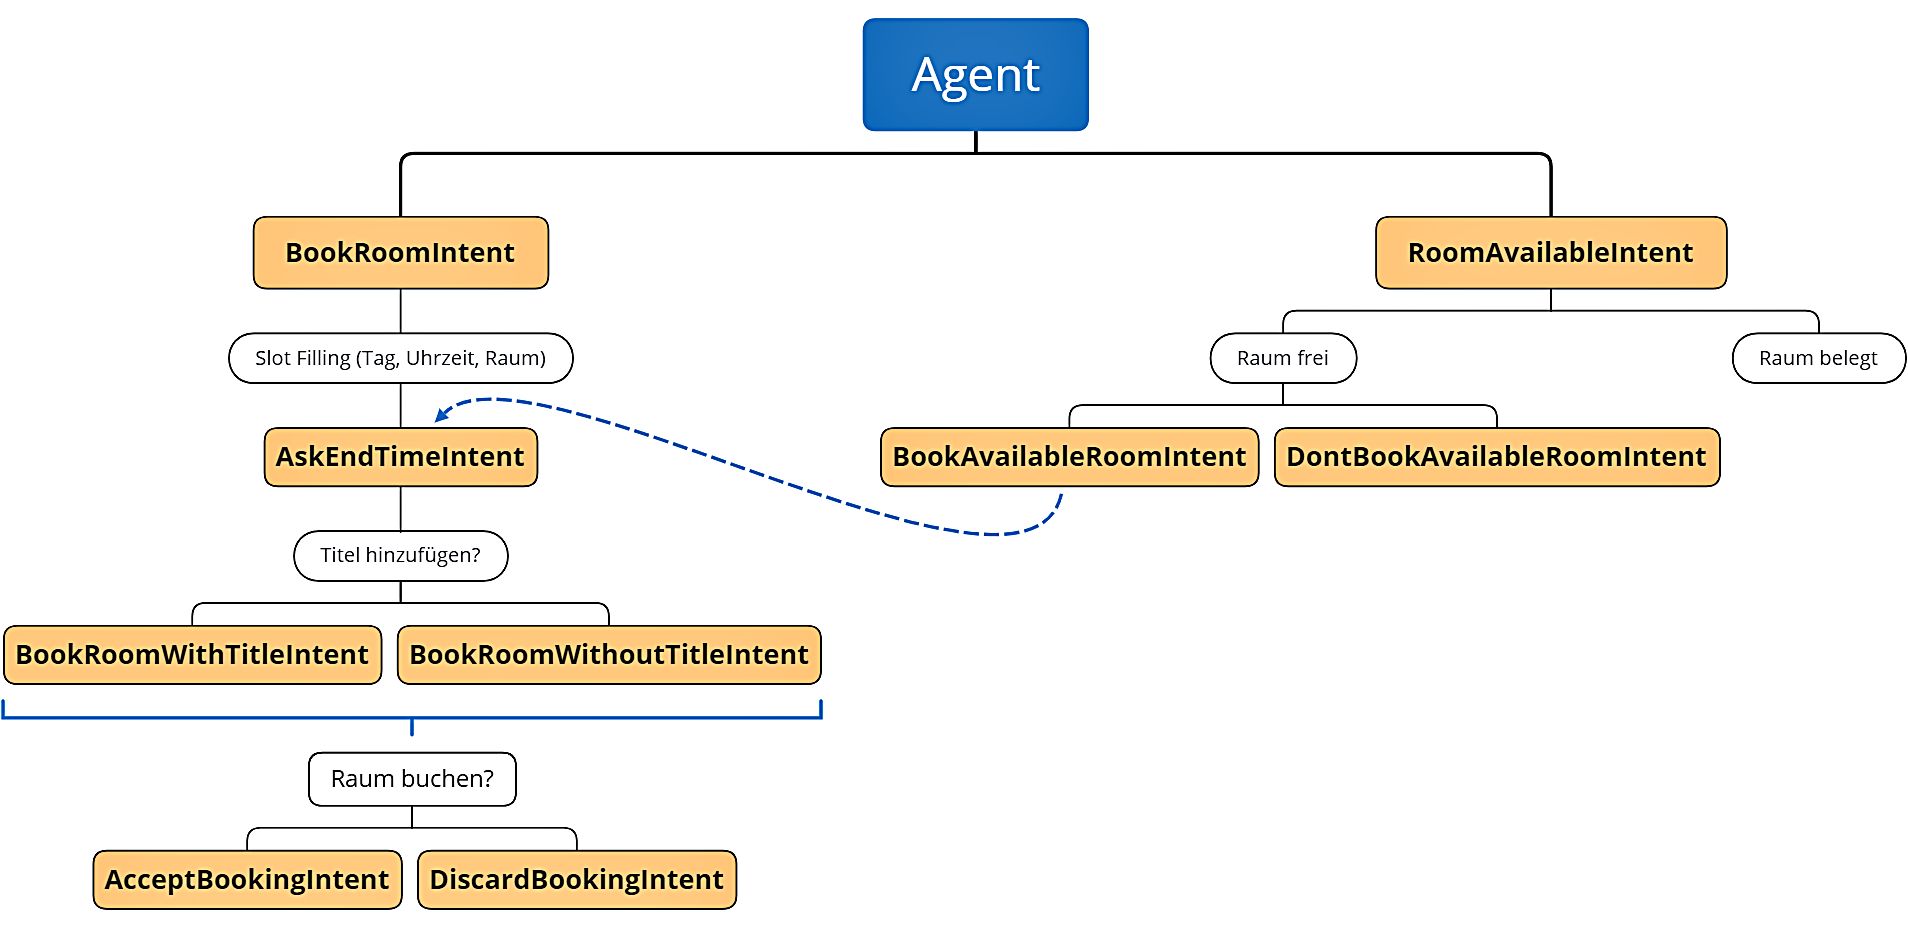
\includegraphics[width=1\textwidth]{bilder/DialogflowIntentStructure_win.PNG}
    \caption{Struktur der Intents im Dialogflow Agent}
    \label{fig:dialogflow-agent-structure}
\end{figure}

Zur Realisierung der Raumbuchung gibt es die beiden Intents \textit{BookRoomIntent} und \textit{RoomAvailableIntent}. Erkennt der Chatbot, dass der Nutzer einen Raum buchen möchte, findet zunächst ein so genanntes \textit{Slot Filling} statt. Dabei werden nach und nach alle für die Buchung notwendigen Parameter abgefragt. Ohne diese Parameter kann im Backend keine Aussage getroffen werden, ob ein oder mehrere Räume zu diesem Zeitpunkt noch frei sind. Ist eine Anfrage in sofern verifiziert, dass alle nötigen Parameter vorhanden sind und der Raum frei ist, springt der Agent in den \textit{AskEndTimeIntent}. Hier wird der Nutzer dann gebeten, eine Endzeit oder Dauer des Termins anzugeben. Anschließend wird noch eine Festlegung zum Titel des Termins getroffen. Wie bereits vorher festgelegt, müssen alle Termine ab 1,5 Stunden einen spezifischen Titel haben. Für kürzere Meetings ist die Angabe eines Titels optional. Möchte der User keinen Titel angeben, wird vom System ein Standardtitel mit der E-Mail-Adresse des Organisators eingetragen. Vor der endgültigen Buchung gibt es noch eine Art \textit{Confirm Message}, mit der der Nutzer die Buchung final bestätigt. 

Möchte der Nutzer dagegen zunächst nur nach einem oder mehreren freien Räumen suchen, wird dies über den \textit{RoomAvailableIntent} realisiert. Wird explizit nach einem Raum gefragt oder ist zu dem gewählten Zeitpunkt nur ein Raum frei, besteht für den User die Möglichkeit, durch einen einfachen Buttonklick direkt in die Buchung des Raums zu springen. Ab hier wiederholt sich dann der zuvor beschriebene Ablauf nach dem \textit{AskEndTimeIntent}. 

\subsection{Entitäten}
\label{subsec:agent-entities}

Im Kontext der Raumbuchung kommen viele, verschiedene Entitäten vor. Wie in Tabelle \ref{tab:nlp-plattform-vergleich} untersucht, werden die relevanten Parameter schon als so genannte \textit{System Entities} von Dialogflow mitgeliefert \cite{dialogflow_system_2018}. Eine Ausnahme stellt hierbei die Entität für den Raum dar. In Dialogflow ist es allerdings problemlos möglich, eigene Entitäten, so genannte \textit{Developer Entities} zu definieren. In der Tabelle \ref{tab:agent-entities} sind alle im Rahmen des Agents verwendeten Entitäten aufgeführt. 
\newline

\begin{table}[H]
\centering
 \begin{tabular}{ | C{2.5cm} || C{1.5cm} || C{4.5cm} || C{4cm} |} 
 \hline
 Name & Art & Beispiel & Beschreibung \\
 \hhline{=::===}
 \hline @sys.date & System & 2018-10-17T12:00:00+02:00 & Datum (ISO-8601)\\ 
 \hline @sys.time & System & 2018-10-17T16:30:00+02:00 & Uhrzeit (ISO-8601)\\ 
 \hline @sys.duration & System & \{"'amount"':1,"'unit"':"'stunde"'\} & Dauer als Objekt \\
 \hline @sys.any & System & Vorstellungsgespräch & Beliebiger Terminname \\ 
 \hline @RoomEntity & Developer & R1 & Name des Raumes \\ 
 \hline
\end{tabular}
\caption{Übersicht der Entitäten des Dialogflow Agents}
\label{tab:agent-entities}
\end{table}

Die Systementitäten \textit{date} und \textit{time} müssen getrennt betrachtet werden. Beide liefern einen Zeitstempel im \textit{ISO-8601 Format}. Im Backend wird dann aus der Information für Datum und Uhrzeit ein kombinierter Zeitstempel errechnet. Für die Dauer des Termins kann der Typ \textit{duration} verwendet werden. Dieser liefert ein Objekt mit einem Integer für den Wert und einem String für die Einheit. Als Titel kann über den Typ \textit{any} ein beliebiger Text eingegeben werden. Die selbst erstellte Entität für die verschiedenen Räume kann den Namen jedes Besprechungsraums beinhalten. Weiterhin gibt es hierbei den Wert \textit{RX}, falls der Nutzer keinen bestimmten Raum buchen möchte.

\section{Node.js Webservice}
\label{sec:nodejs-webservice}

Wie bereits in \ref{subsec:webservice} beschrieben, wird für die Implementierung des Backends Node.js verwendet. Auf das Backend kommen in diesem Fall mehrere Aufgaben zu. Es erhält über einen so genannten Webhook ein von Dialogflow generiertes \ac{JSON}-Objekt. In diesem Objekt sind alle für die aktuelle Session relevanten Daten aufgelistet. Da nicht alle von Dialogflow mitgelieferten Daten relevant sind, wird zunächst über einen \textit{Callback} ein Objekt generiert, in dem alle relevanten Daten zur Useranfrage abgelegt sind. Die relevanten Daten sind in Tabelle \ref{tab:data-dialogflow-json} aufgelistet.
\newline

\begin{table}[H]
\centering
 \begin{tabular}{ | C{3cm} || C{1.5cm} || C{8cm} |} 
 \hline
 Name & Art & Beschreibung \\
 \hhline{=::==}
 \hline session\_id & String & Identifier zur Zuordnung zu User aus Datenbank \\ 
 \hline intent\_id & String  & Eindeutiger Identifier für den Intent \\ 
 \hline intent\_name & String & Name des Intents \\
 \hline parameters & Object  & Sämtliche relevante Parameter, z.B. time, date, etc. \\ 
 \hline
\end{tabular}
\caption{Relevante Daten aus Dialogflow \acs{JSON}-Request}
\label{tab:data-dialogflow-json}
\end{table}

Weiterhin wird eine Datenbankanbindung benötigt, in der die Daten der User gespeichert und verwaltet werden. Die Zuordnung im Rahmen der Anfragen von Dialogflow geschieht durch die Session-\ac{ID}. Jeder Datenbankeintrag besitzt eine universelle \mbox{Person-\ac{ID}}, über die der Eintrag einem User zugeordnet werden kann. Zudem sind die E-Mail-Adresse und der Vorname des Nutzers hinterlegt. Über die abgespeicherten Token kann anschließend ein Zugriff auf die Kalenderereignisse stattfinden. Der Wert für das \textit{expiry date} dient dem internen Handling zur Überprüfung der Gültigkeit und Erneuerung des \textit{access token}. Eine Übersicht aller Parameter zu einem Nutzereintrag in der Datenbank ist in Tabelle \ref{tab:data-datenbank} dargestellt.
\newline

\begin{table}[H]
\centering
 \begin{tabular}{ | C{3cm} || C{1.5cm} || C{7cm} |} 
 \hline
 Name & Art & Beschreibung \\
 \hhline{=::==}
 \hline session\_id & String & Identifier zur Zuordnung des Users \\ 
 \hline person\_id & String & Eindeutiger Identifier des Google-Accounts \\ 
 \hline email & String & E-Mail-Adresse des Users \\ 
 \hline given\_name & String & Vorname des Users \\ 
 \hline access\_token & String & Zugriffs Token des Users \\ 
 \hline refresh\_token & String & Refresh Token des Users \\
 \hline expiry\_date & Number  & Ablaufdatum des Tokens \\ 
 \hline
\end{tabular}
\caption{Parameter aus der Datenbank}
\label{tab:data-datenbank}
\end{table}

Die Anbindung der \textit{Google Calendar \ac{API}} zum Abfragen und Erstellen von Terminen ist ebenso Aufgabe des Webservices. Die Google Calendar \ac{API} kann dabei sowohl für den Eintrag in den Kalender des Users, als auch für die Abfrage der Besprechungsräume im Office der \adorsys\ verwendet werden. Die Räume sind dabei als Ressourcen innerhalb der Domäne der Firma angelegt und über eine kryptische E-Mail-Adresse ansprechbar. Abfragen von freien Zeiträumen und Einträge in die Terminkalender können dann gemäß \cite{google_developers_node.js_2018} und \cite{google_developers_create_2018} getätigt werden.

Um die Einträge in der Datenbank auf dem aktuellen Stand zu halten, müssen die aktuelle Session-\ac{ID} und der zum Nutzer gehörige Android-\ac{ID}-Token über eine \ac{HTTP}-Nachricht von der Android App an das Backend geschickt werden. Auf die gleiche Weise wird auch der Authentifizierungscode versendet, aus dem anschließend im Backend die Token für den Kalenderzugriff generiert werden. Für diese Funktionalitäten werden im Backend so genannte Endpunkte definiert. Um dies zu realisieren wird das Node.js-Framework \textit{Express} verwendet. Damit kann relativ einfach und minimalistisch eine \ac{REST}-Schnittstelle umgesetzt werden. Es wird dazu jeweils eine \textit{POST-Methode} zum Verifizieren von Session-\ac{ID} und Android-\ac{ID}-Token, sowie der Auswertung des Authentifizierungscodes implementiert.

Im Backend findet mit den von Dialogflow gelieferten Daten sozusagen das \acl{DM} statt. Welches \ac{UI}-Element die Android App am Ende als Antwort für den User anzeigen soll, ist durch ein \ac{JSON}-Objekt definiert. Dabei gibt es die Möglichkeit, Daten über einen so genannten \textit{payload} durch Dialogflow durchzuschleifen. Ein Beispiel der Darstellung des \ac{UI}-Elements im Backend zeigt Listing \ref{lst:json-payload}.
\newline

\begin{lstlisting}[caption={Darstellung des \acs{UI}-Elements im Backend im \acs{JSON}-Format}, captionpos=b, label={lst:json-payload}, language=myjson]
"payload": 
{
    "android": 
	 {
        "type": "button",
        "text": "Soll dein Termin einen Titel haben?"
	 }
}
\end{lstlisting}

Zur Unterscheidung der unterschiedlichen \ac{UI}-Elemente dient hierbei der \textit{type}. In Listing \ref{lst:json-payload} ist dies ein \textit{button}, der im Frontend eine Phrase und die Auswahlbuttons \textit{Ja}/\textit{Nein} darstellt. Der \textit{text} repräsentiert an dieser Stelle die Phrase, die der Nutzer als Antwort erhält und ist für alle \ac{UI}-Elemente notwendig. Anstelle von \textit{button} kann an dieser Stelle auch \textit{textmessage} oder \textit{slider} angegeben werden. Die Zuordnung ist analog zu der im Unterkapitel \nameref{subsec:Chat Interface} angegebenen Tabelle \ref{tab:arten-nachrichten-chat-interface}.

Auf diese Art und Weise können nun beliebig viele, weitere \ac{UI}-Elemente definiert und umgesetzt werden. Dabei muss natürlich das entsprechende \ac{UI}-Element auch in der Android App bekannt und implementiert sein. Als erstes Modell und zum Datenaustausch funktioniert dies auch problemlos. Jedoch erscheinen zukünftige Probleme nicht unvermeidbar. Über die gewählte Architektur und den Komponentenaufbau aus \ref{sec:auswahl-komponenten} müssen die entsprechenden Daten immer durch Dialogflow hindurch geschleust werden. Ändert sich hierbei der Aufbau des \ac{JSON}-Objekts oder wird gar das Durchschleifen von Daten unterbunden, so muss die gewählte Vorgehensweise geändert werden oder ist im schlimmsten Fall gar nicht mehr realisierbar. Als Anregung sei in diesem Zusammhang erwähnt, dass die Komponenten \textit{Webservice} und \textit{\ac{NLP}-Plattform} in ihrer Anordnung auch vertauscht werden könnten. Dies hätte den Vorteil, dass Dialogflow nur noch für das \textit{\acl{NLU}} zuständig wäre und keine Daten darüber mitgeschleift werden müssen. Diese Ansätze werden allerdings nicht weiter beleuchtet, sondern dienen lediglich als kritische Hinterfragung der eigenen Struktur.

Abschließend sollen alle für das System relevanten Komponenten und der damit verbundene Ablauf vom Senden einer Nachricht durch den User bis zur Rückmeldung einer Nachricht in der App anhand eines Sequenzdiagramms dargestellt werden. Anzumerken ist hierbei, dass dieses Diagramm natürlich nicht für alle Anwendungsfälle gleich ist. Es soll vielmehr die Hintergründe anhand eines typischen und häufig vorkommenden Use Cases, wie beispielsweise der Abfrage eines freien Raumes, verdeutlichen. Das entsprechende Sequenzdiagramm ist in Abbildung \ref{fig:sequence-diagramm-basic-system-interaction} dargestellt.
\newline

\begin{figure}[H]
    \centering
    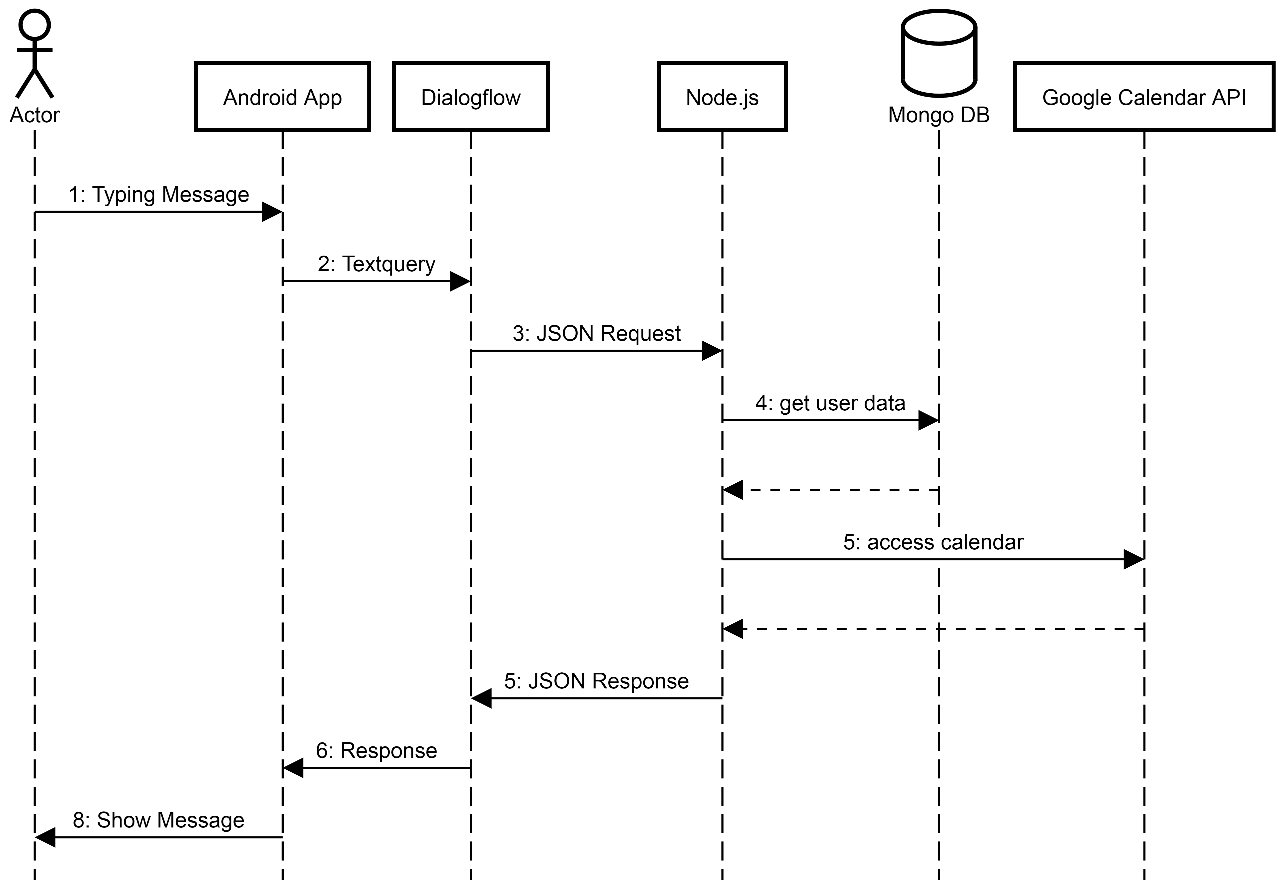
\includegraphics[width=1\textwidth]{bilder/Basic-System-Interaction.png}
    \caption{Sequenzdiagramm zur Interaktion der Systeme}
    \label{fig:sequence-diagramm-basic-system-interaction}
\end{figure}

In der Android Applikation tippt der User zunächst eine Nachricht ein oder bedient sich eines bereits vorhandenen \ac{UI}-Elements und sendet so eine textuelle Nachricht an Dialogflow. Dort wird die Nachricht mit Hilfe von \acl{NLU} interpretiert und gelangt über den Webhook an den Node.js Server. Anhand der hinterlegten Session-\ac{ID} können die relevanten Informationen und Zugriffstoken aus einer MongoDB Datenbank gelesen werden. Sind alle Zugriffsrechte vorhanden, können über die Google Calendar \ac{API} freie Räume abgefragt oder gebucht werden. Eine entsprechende Rückmeldung sendet der Webservice mit Hilfe einer \ac{JSON}-Response an Dialogflow. Über die in der Android App eingebundene Bibliothek gelangt die Antwort letztendlich zurück zum User und wird ihm entsprechtend als Text oder \ac{UI}-Element angezeigt.


\chapter{Schlussbetrachtung}
\label{cha:schlussbetrachtung}

Im folgenden Kapitel wird die gesamte Arbeit rekapituliert. Dabei wird anhand der Vorgehensweise nochmals auf die wichtigsten Erkenntnisse eingegangen und diese erläutert. Anhand eines kurzen Ausblicks werden Anregungen für weitere Untersuchungen gegeben.

\section{Fazit}
\label{sec:fazit}

Gegenstand der Arbeit war die Konzeptionierung und Implementierung einer Android Applikation zur Raumbuchung via \acl{CUI}. Dazu wurden zunächst die Anforderungen an ein \ac{CUI} im Allgemeinen und auch im Kontext der Raumbuchung mit Hilfe von Methoden aus dem Bereich Usability Engineering betrachtet. 

In diesem Zusammenhang konnten mit Hilfe eines Fragebogens, Interviews und der Entwicklung von Personae ausführliche Einblicke in das Buchungsverhalten der Nutzer gewonnen werden. Hierbei wurde klar, dass die Ziele und Absichten der User sehr kontextspezifisch sind. So hat beispielsweise ein Mitarbeiter aus dem Bereich \textit{Human Resources} ein ganz anderes Verhalten und Präferenzen bei der Buchung als jemand aus dem Bereich \textit{Coaching}. Schnell wurde deutlich, dass diese Unterschiede erkannt und verinnerlicht werden müssen, bevor ein sinnvolles und zielgerichtetes Protoyping überhaupt stattfinden kann. 

Anhand von Papier-Prototypen und deren anschließender Umsetzung anhand eines Klickdummys konnten die ersten Ansätze auf ihre Plausibilität hin untersucht werden, bevor sie dann im Prototyping Tool umgesetzt wurden. Diese verschiedenen Ebenen des Prototypings sind eine gute Hilfe, um am Anfang uneingeschränkt und kreativ Ideen aufbringen zu können, diese anschließend möglichst schnell einem \textit{plausibility check} zu unterziehen und abschließend zu entscheiden, ob diese weiterverfolgt oder verworfen werden. 

Anschließend stand der Workflow, also die Vorgehensweise vom Anfang bis zum Abschluss der Buchung, im Vordergrund. Hierfür wurden auf Grundlage der Ergebnisse aus dem Requirements Engineering und in Anlehnung an die entwickelten Personae verschiedene Szenarien entworfen. Für jedes Szenario wurden dabei die unterschiedlichen Möglichkeiten und Wege bis zum Ende der Buchung betrachtet und anhand von Entscheidungsbäumen dargestellt. Dabei wurde deutlich, dass es je nach Art des Szenarios große Unterschiede in Bezug auf die Variation der Nutzeranfrage gibt. Im Kapitel \ref{subsec:workflow} wurde dabei zum einfacheren Verständnis das weniger umfangreiche Szenario aus dem Bereich \textit{Vertrieb} gewählt. Für ein anderes Szenario steigt der Umfang der möglichen Eingangsformulierungen des Users allerdings schnell auf bis zu zwölf Zweige an. Dies verdeutlicht die enorme Variabilität des Nutzers bei der Verwendung eines \aclp{CUI}.

Durch die Umsetzung der Ansätze mit Hilfe des Prototyping Tools werden schnell Probleme beim Workflow oder im mentalen Modell des Nutzers erkannt. Der Vorteil ist hierbei, dass diese Probleme noch im Status der Konzeption bzw. im Prototyping behoben werden können. In Abbildung \ref{fig:kosten-fehlerbehebung-softwareentwicklung} sind die Kosten der Fehlerbehebungen in der Softwareentwicklung über die verschiedenen Entwicklungsphasen dargestellt. Die Vorgehensweise nach dem Motto \textit{„test early - fail early“} spart hierbei also sowohl Zeit und Aufwand, als auch Kosten.
\newline
\begin{figure}[H]
    \centering
    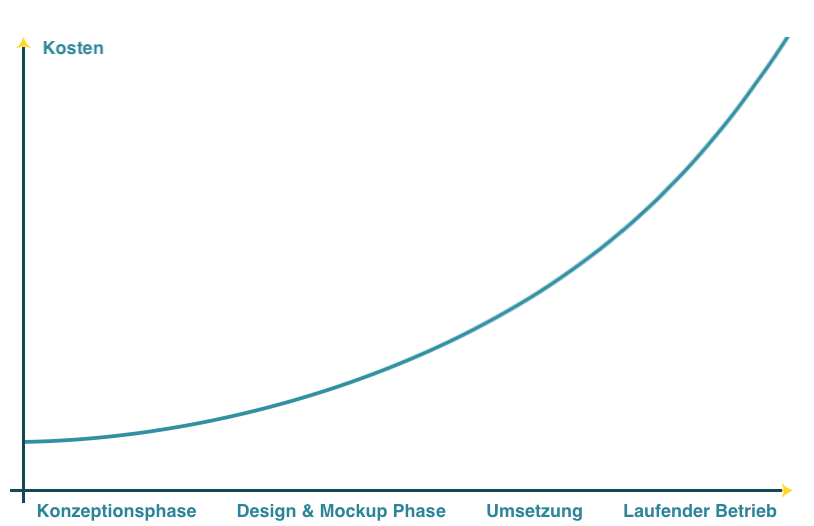
\includegraphics[width=0.9\textwidth]{bilder/fehlerkostensoftware.png}
    \caption{Kosten der Fehlerbehebung in der Softwareentwicklung \cite{claus_degendorfer_wie_2016}}
    \label{fig:kosten-fehlerbehebung-softwareentwicklung}
\end{figure}

Die prinzipielle Idee eines \acl{CUI} mit der Kombination aus Text und \ac{UI}-Elementen im Kontext einer Raumbuchung ist für die Nutzer verständlich. Dies bestätigen die Ergebnisse und Rückmeldungen aus den User Tests. Zudem bieten diese gute Ansatzpunkte für eine weitere Bearbeitung der Thematik. Darauf soll explizit noch im Folgekapitel \textit{\nameref{sec:ausblick}} eingegangen werden.

Wie auch dem Umfang der entsprechenden Kapitel \textit{\nameref{cha:konzeption}} und \textit{\nameref{cha:implementierung}} zu entnehmen ist, stellt die konzeptionelle Betrachtung einen großen Teil der Arbeit dar. Wie zuvor erläutert ist dies gleichermaßen wichtig wie notwendig, um ein fundiertes Verständnis über die Thematik zu erhalten. Nichtsdestotrotz ist auch die Implementierung ein fester Bestandteil der Arbeit und wurde entsprechend umgesetzt. Durch die Auswahl der Komponenten und deren Aufbau sowie die Klärung ihrer Kommunikation und Schnittstellen konnte hierbei ein solides Grundgerüst für eine weitere Implementierung aufgebaut werden. Einige der im Prototyping erprobten Ansätze in Bezug auf den Konversationsfluss und der \ac{UI}-Elemente konnten hierbei bereits einfließen. Dem Nutzer ist es möglich, mit Hilfe der Android Applikation nach freien Räumen im Office der \adorsys\ zu suchen und einen Besprechungsraum zu reservieren.

\section{Ausblick}
\label{sec:ausblick}
Aufgrund des begrenzten Zeitrahmens in Abschlussarbeiten können meist leider nicht alle Inhalte einer Thematik ausreichend beleuchtet oder umgesetzt werden. Daher dient dieses Unterkapitel dazu, einige Anmerkungen und Ausblicke für weitere Betrachtungen aufzugreifen und zu erläutern. 

Wie bereits eingangs erwähnt, dient Sprache sowohl der schriftlichen als auch der mündlichen Konversation. In dieser Arbeit lag der Fokus auf der Entwicklung eines textuellen \acp{CUI} in Form eines Chatbots. Denkbar wäre hier also eine Erweiterung des Systems um eine sprachbasierte Eingabemöglichkeit. Dabei wird die gesprochene Sprache über ein Mikrofon aufgenommen und über \textit{\ac{ASR}} in Textform konvertiert. Die textuelle Sprache kann anschließend weiter verarbeitet werden. Der Rückweg zur Ausgabe des Audiosignals wird dann mit Hilfe von \textit{\ac{TTS}} realisiert.

Während der Durchführung der User Tests kam häufig die Frage nach einem Namen oder dem Aussehen des Chatbots auf. Viele Nutzer haben einen Charakter des Chatbots erwartet oder gar vermisst. In diesem Zusammenhang erscheint ein Charakterdesign für den Chatbot als sinnvoll. Dabei erhält der Chatbot einen Namen und einen Avatar, was ihn für den User transparenter und sympathischer macht. 

Nahezu unverzichtbar ist für den Kontext einer Raumbuchung natürlich die Einladung von weiteren Personen. Dieser Teil wurde im Rahmen der Arbeit bewusst zunächst außen vor gelassen, muss aber früher oder später fester Bestandteil des Systems sein. Großen Mehrwert hat das System hier bei der Terminfindung. So können beispielweise alle Teilnehmer eines Meetings angegeben und der nächstmögliche freie Termin inklusive passendem Raum vorgeschlagen werden. Eine ergänzende Idee ist hierbei, im System gewisse Teams zu hinterlegen. So könnte der User beispielsweise nur angeben, er möchte alle Mitglieder aus dem \textit{iOS-Team} zu einem Termin einladen und das System schlägt ihm mögliche Zeiträume vor, bei dem alle oder zumindest ein Großteil der Teilnehmer verfügbar ist. 

Enormes Potenzial für den Anwendungsfall der Raumbuchung bietet auch die Technologie des \aclp{ML}. Bis zum derzeitigen Stand der Arbeit befindet sich \acl{ML} nur im Bereich der \ac{NLP}-Plattform. Dies passiert jedoch unter der Oberfläche von Dialogflow und stellt somit keinen direkten Berührungspunkt dar. Eine eigene Umsetzung aus dem Bereich \ac{ML} im Rahmen des \aclp{DM} könnte die Intelligenz des Systems wesentlich verbessern. Ein mögliches Anwendungsgebiet ist hierbei das Erkennen und Erlernen von Verhaltensmustern eines Nutzers bei der Buchung. Damit wäre das System in der Lage, für einen Nutzer spezifische Vorhersagen über die Raumpräferenzen oder die Auswahl von Vor- und Nachbereitungszeit für einen Termin zu treffen. 

% alle Glossareinträge werde automatisch angezeigt (auch wenn sie nicht verwendet werden) -> dadurch müssen sie nicht expliztit mit \gls{} aufgerufen werden
%\csappto{theglossary}{\label{cha:glossar}}
%\printglossaries    

\small
%\bibliographystyle{literatur/IEEEtran} standard
\bibliographystyle{literatur/alpha} % added by mwa
\bibliography{literatur/Bibliographie}

\normalsize

%\addchap{Eidesstattliche Erklärung}

Ich, \autor, Matrikel-Nr.\ \matrikelnr, versichere hiermit, dass ich meine Masterarbeit mit dem Thema
\begin{quote}
\textit{\titel}
\end{quote}
selbständig verfasst und keine anderen als die angegebenen Quellen und Hilfsmittel benutzt habe, wobei ich alle wörtlichen und sinngemäßen Zitate als solche gekennzeichnet habe. Die Arbeit wurde bisher keiner anderen Prüfungsbehörde vorgelegt und auch nicht veröffentlicht.

Mir ist bekannt, dass ich meine Masterarbeit zusammen mit dieser Erklärung fristgemäß nach Vergabe des Themas in dreifacher Ausfertigung und gebunden im Prüfungsamt der Ohm-Hochschule abzugeben oder spätestens mit dem Poststempel des Tages, an dem die Frist abläuft, zu senden habe.\\[6ex]

\ort, den \today


\rule[-0.2cm]{5cm}{0.5pt}

\textsc{\autor} 


\begin{appendix}
    \clearpage
    \pagenumbering{roman}
    \chapter{Anhang}
    \label{sec:Anhang}
    % Rand der Aufzählungen in Tabellen anpassen
    \setdefaultleftmargin{1em}{}{}{}{}{}
    \section{Ergebnisse des Fragebogens}
\label{sec:anhang-fragebogen}

Im Folgenden werden die Fragen und Antworten des Online Fragebogens ausführlich dargestellt. Die Anzahl der Teilnehmer kann dabei variieren, da manche Fragen als Pflichtfragen deklariert wurden und andere nicht. Ob die Frage eine Pflichtfrage ist, Single- oder Multiple-Choice und wie viele der Teilnehmer die Frage beantwortet haben, ist jeweils nachstehend kurz angegeben.

\begin{enumerate}
    \item \textbf{Wie häufig buchst du einen Raum?} \\
    Pflichtfrage, Single-Choice, Anzahl Teilnehmer: 46
    \begin{itemize}
        \item[] 6 (13,0\,\%): täglich
        \item[] 14 (30,4\,\%): alle 2-3 Tage
        \item[] 10 (21,7\,\%): wöchentlich
        \item[] 9 (19,6\,\%): monatlich
        \item[] 7 (15,2\,\%): nie
    \end{itemize}
    
    \item \textbf{Wie lange im Voraus buchst du in der Regel einen Raum?} \\ 
    Pflichtfrage, Single-Choice, Anzahl Teilnehmer: 46
    \begin{itemize}
        \item[] 4 (8,7\,\%): unmittelbar
        \item[] 4 (8,7\,\%): am selben Tag
        \item[] 11 (23,9\,\%): ein Tag
        \item[] 17 (37,0\,\%): mehrere Tage
        \item[] 1 (2,2\,\%): Wochen/Monate
        \item[] 9 (19,6\,\%): Ich habe noch nie einen Raum gebucht
    \end{itemize}
    
    \item \textbf{Wie lange dauern deine Besprechungen in der Regel?} \\ 
    Keine Pflichtfrage, Single-Choice, Anzahl Teilnehmer: 46
    \begin{itemize}
        \item[] 13 (28,3\,\%): < 1 Std.
        \item[] 30 (65,2\,\%): 1 - 2 Std.
        \item[] 3 (6,5\,\%): 2 - 3 Std.
        \item[] 0 (0,0\,\%): 3 - 4 Std.
        \item[] 0 (0,0\,\%): > 4 Std.
    \end{itemize}
    
    \item \textbf{Wie oft stimmt die gebuchte Dauer eines Termins mit der tatsächlichen überein?} 
    \\ 
    Keine Pflichtfrage, Single-Choice, Anzahl Teilnehmer: 38
    \begin{itemize}
        \item[] 9 (23,7\,\%): sehr oft
        \item[] 21 (55,3\,\%): oft
        \item[] 3 (7,9\,\%): ausgeglichen
        \item[] 5 (13,2\,\%): selten
        \item[] 0 (0,0\,\%): sehr selten
    \end{itemize}
    
    \item \textbf{Wie oft wird ein Meeting beendet, weil die Buchung des Raums abgelaufen ist, obwohl noch Gesprächsbedarf bestehen würde?} \\ 
    Keine Pflichtfrage, Single-Choice, Anzahl Teilnehmer: 38
    \begin{itemize}
        \item[] 1 (2,6\,\%): sehr oft
        \item[] 7 (18,4\,\%): oft
        \item[] 10 (26,3\,\%): ausgeglichen
        \item[] 15 (39,5\,\%): selten
        \item[] 5 (13,2\,\%): sehr selten
    \end{itemize}
    
    \item \textbf{Hast du beim Buchen von Räumen einen festen oder flexiblen Zeitpunkt?} \\ 
    Keine Pflichtfrage, Single-Choice, Anzahl Teilnehmer: 44
    \begin{itemize}
        \item[] 4 (9,1\,\%): fest
        \item[] 8 (18,2\,\%): eher fest
        \item[] 19 (43,2\,\%): ausgeglichen
        \item[] 7 (15,9\,\%): eher flexibel
        \item[] 6 (13,6\,\%): flexibel
    \end{itemize}
    
    \item \textbf{Wie oft benutzt du den Slackbot Joan?} \\ 
    Pflichtfrage, Single-Choice, Anzahl Teilnehmer: 46
    \begin{itemize}
        \item[] 1 (2,2\,\%): jede Buchung
        \item[] 2 (4,3\,\%): eher fest
        \item[] 2 (4,3\,\%): ausgeglichen
        \item[] 0 (0,0\,\%): Selten
        \item[] 41 (89,1\,\%): nie
    \end{itemize}
    
    \item \textbf{Nutzt du das E-Paper Display an den Räumen, wenn du sofort einen Raum benötigst?} \\ 
    Pflichtfrage, Single-Choice, Anzahl Teilnehmer: 46
    \begin{itemize}
        \item[] 16 (34,8\,\%): immer
        \item[] 15 (32,6\,\%): oft
        \item[] 5 (10,9\,\%): ausgeglichen
        \item[] 5 (10,9\,\%): selten
        \item[] 5 (10,9\,\%): nie
    \end{itemize}
    
    \item \textbf{Nutzt du das E-Paper Display an den Räumen, wenn zu einem späteren Zeitpunkt den Raum verwenden möchtest} \\ 
    Pflichtfrage, Single-Choice, Anzahl Teilnehmer: 46
    \begin{itemize}
        \item[] 1 (2,2\,\%): immer
        \item[] 3 (6,5\,\%): oft
        \item[] 5 (10,9\,\%): ausgeglichen
        \item[] 9 (19,6\,\%): selten
        \item[] 28 (60,9\,\%): nie
    \end{itemize}
    
    \item \textbf{Wie oft stimmt deiner Erfahrung nach der Belegungsstatus des Raumes mit den Angaben auf dem E-Paper Display überein?} \\ 
    Pflichtfrage, Single-Choice, Anzahl Teilnehmer: 46
    \begin{itemize}
        \item[] 3 (6,5\,\%): immer
        \item[] 11 (23,9\,\%): oft
        \item[] 21 (45,7\,\%): ausgeglichen
        \item[] 11 (23,9\,\%): selten
        \item[] 0 (0,0\,\%): nie
    \end{itemize}
    
    \item \textbf{Wie oft benötigst du bei deinen Meetings bestimmtes Equipment?} \\
    Gemeint ist damit Equipment, das nicht standardmäßig in den Räumen vorhanden ist, also etwas anderes als AppleTV, Fernseher, Whiteboard. \\ 
    Pflichtfrage, Single-Choice, Anzahl Teilnehmer: 46
    \begin{itemize}
        \item[] 1 (2,2\,\%): immer
        \item[] 19 (41,3\,\%): oft
        \item[] 5 (10,9\,\%): ausgeglichen
        \item[] 15 (32,6\,\%): selten
        \item[] 6 (13,0\,\%): nie
    \end{itemize}
    
     \item \textbf{Wie führst du deine Raumbuchungen aktuell am häufigsten durch?} \\ 
     Pflichtfrage, Single-Choice, Anzahl Teilnehmer: 46
    \begin{itemize}
        \item[] 39 (84,8\,\%): Computer - Web Interface
        \item[] 7 (15,2\,\%): Ich habe noch nie einen Raum gebucht
        \item[] 0 (0,0\,\%): Smartphone - Web Interface
        \item[] 0 (0,0\,\%): Slackbot Joan
    \end{itemize}
    
    \item \textbf{Wie würdest du deine Raumbuchung am liebsten durchführen?} \\ 
    Pflichtfrage, Single-Choice, Anzahl Teilnehmer: 46
    \begin{itemize}
        \item[] 34 (73,9\,\%): Computer - Web Interface
        \item[] 5 (10,9\,\%): Smartphone - Applikation
        \item[] 3 (6,5\,\%): Computer - Anwendung
        \item[] 3 (6,5\,\%): Slackbot Joan
        \item[] 1 (2,2\,\%): Smartphone - Web Interface
    \end{itemize}
    
    \item \textbf{Wie fändest du es, wenn du die Raumbuchung bestätigen müsstest?} \\ 
    Pflichtfrage, Single-Choice, Anzahl Teilnehmer: 46
    \begin{itemize}
        \item[] 11 (23,9\,\%): gut
        \item[] 15 (32,6\,\%): eher gut
        \item[] 6 (13,0\,\%): neutral
        \item[] 6 (13,0\,\%): eher schlecht
        \item[] 8 (17,4\,\%): schlecht
    \end{itemize}
    
    Begründungen:
    \begin{itemize}
        \item ich nicht weiß ob immer daran denke [Auswahl: neutral]
        \item ich sicherlich nicht daran denke, denn nach der Raumbuchung (die nicht abgelehnt wird) ist die Sache bei mir abgehakt [Auswahl: schlecht]
        \item Dann Räume auch wieder frei werden, allerdings sollte das Zeitintervall schon auch ein paar Minuten -> 15/20 tolerieren [Auswahl: eher gut]
        \item der Raum bei nicht Benutzung als frei markiert ist somit weiter verwendbar [Auswahl: eher gut]
        \item weil dann sicher ist welches Meeting in dem Raum ist, falls man zb zu spät kommt, wissen will das genau das meeting um zb 13 Uhr zu ende ist,... [Auswahl: eher gut]
        \item dadurch der Raum nicht leerstehen würde [Auswahl: eher gut]
        \item Räume sind beschränkte Ressource und es kann immer etwas dazwischen kommen [Auswahl: gut]
        \item Räume die nicht bestätigt werden, auch wieder freigegeben werden können [Auswahl: gut]
        \item so vermieden wird, das unnötig Räume gebucht werden, die danach doch nicht gebraucht werden und leer stehen [Auswahl: eher gut]
        \item Bei nicht Bestätigung wird der Raum sofort wieder freigegeben [Auswahl: gut]
        \item nicht bestätigte Räume wieder freigegeben werden und somit wieder nutzbar für andere Kollegen sind [Auswahl: gut]
        \item sichergestellt wird, dass der Raum auch gebraucht wird und keine Leerbuchung stattfindet [Auswahl: eher gut]
        \item gebuchte Räume, die nicht verwendet werden Verschwendung sind [Auswahl: eher gut]
        \item der Raum dann bei kurzfristigen Änderungen nicht unnötig vergeben bleibt [Auswahl: gut]
        \item genug zu tun und eh zuviel spam [Auswahl: eher schlecht]
        \item es mir vorkommt, als müsste ich die Buchung 2x durchführen [Auswahl: schlecht]
        \item Zeitraubend, überflüßig [Auswahl: eher schlecht]
        \item Außenstehende dann sofort wissen, ob das Meeting wirklich stattfindet oder nicht [Auswahl: eher gut]
        \item Sonst gebuchte Räume leer stehen [Auswahl: eher gut]
        \item Verstehe die Frage nicht das muss man jetzt ja auch? [Auswahl: gut]
        \item leer stehende Räume vermieden werden können [Auswahl: neutral]
        \item zusaetzlicher Aufwand + wozu? [Auswahl: schlecht]
        \item der Raum dann wieder freigegeben wird, wenn nicht genutzt [Auswahl: eher gut]
        \item zu aufwendig [Auswahl: schlecht]
        \item Overhead [Auswahl: eher schlecht]
        \item kurzer Aufwand für mehr Klarheit [Auswahl: gut]
        \item dann sicher festgestellt werden kann, das der Raum auch tatsächlich benutzt wird und die Raum ansonsten für andere Personen wieder zur Verfügung steht [Auswahl: gut]
        \item man dann die genaue Anzahl an Teilnehmer weiß [Auswahl: gut]
        \item doppelte Arbeit [Auswahl: schlecht]
        \item ich finde, dass das niemand hilft. Das größte Problem bei uns, dass man ohne Buchung Räume besitzt [Auswahl: schlecht]
        \item weniger Probleme mit Fehlbuchungen und ungenutzten Räumen [Auswahl: gut]
        \item mehr darüber nachgedacht werden würde, ob der Raum tatsächlich benötigt wird oder ob sich das Meeting erledigt hat [Auswahl: eher gut]
    \end{itemize}
    
    \item \textbf{Gibt es bevorzugte Räume bei deiner Buchung?} \\ 
    Keine Pflichtfrage, Multiple-Choice, Anzahl Teilnehmer: 25
    \begin{itemize}
        \item[] 14 (56,0\,\%): Raum R1
        \item[] 15 (60,0\,\%): Raum R2
        \item[] 7 (28,0\,\%): Raum R3
        \item[] 14 (56,0\,\%): Raum R4
        \item[] 3 (12,0\,\%): Raum R6
    \end{itemize}
    
    Begründungen:
    \begin{itemize}
        \item wir oft Konferenzen mit Mitarbeitern haben, die nicht im Office vorort sind [Auswahl: R3]
        \item R4 - nicht einfach einsehbar -> privater [Auswahl: R2;R4]
        \item nicht zu großer Raum [Auswahl: R1;R2;R4]
        \item Perfekte Anzahl von Sitzplätzen und Raumgröße [Auswahl: R1;R2]
        \item meine Meetings nicht so groß sind, und ich meistens keine ViCo brauche (Auswahl: R1;R2;R4]
        \item ausreichend Platz um sich mit Leuten darin zu bewegen und ausreichend Schreibfläche [Auswahl: R4]
        \item Whiteboard, TV, Stühle [Auswahl: R1;R2]
        \item am angenehmsten , R6 nur für große Meetings, R1,R2 komische Tische [Auswahl: R3]
        \item Gute Atmosphäre, Klimanalge perfekt, Tische und Ausstattung am besten, Gutes Licht! (negativ beispiel R3 Videoraum...) [Auswahl: R1; R4]
        \item passen gut zu meinen Meetings [Auswahl: R1;R2;R4]
        \item Kleinere Räume [Auswahl: R1;R2;R3;R6]
        \item großer Kreis an Leuten, häufig auch Workshops [Auswahl: R4;R6]
        \item es mit Videokonferenzsystem aufgebaut ist [Auswahl: R3]
        \item es dort hell ist, es gibt Fenster und man wird von außen nicht so beobachtet [R1;R2;R4]
    \end{itemize}
    
    \item \textbf{Welche Kriterien sind für dich bei der Raumbuchung relevant?} \\ 
    Pflichtfrage, Multiple-Choice, Anzahl Teilnehmer: 46
    \begin{itemize}
        \item[] 41 (89,1\,\%): Anzahl der Personen
        \item[] 25 (54,3\,\%): Art der Besprechung
        \item[] 19 (41,3\,\%): Ausstattung
        \item[] 18 (39,1\,\%): Dauer der Besprechung
        \item[] [Anmerkung]
        \item[] Für die folgenden Punkte stimmte je ein Teilnehmer (2,2\,\%)
        \begin{itemize}
            \item Diskretion (dass man in den Raum nicht reinschauen kann + den Bildschirm nicht lesen kann)
            \item Platz zum bewegen, Schreibfläche und Sichtbarkeit der Schreibfläche für alle (nichts gedrängtes)
            \item Teilnehmer außerhalb des Offices?
        \end{itemize}
    \end{itemize}
    
    \item \textbf{Worin besteht dein Haupttätigkeitsfeld?} \\ 
    Pflichtfrage, Single-Choice, Anzahl Teilnehmer: 46
    \begin{itemize}
        \item[] 20 (43,5\,\%): Entwicklung
        \item[] 8 (17,4\,\%): Projektleitung
        \item[] 4 (8,7\,\%): HR
        \item[] 3 (6,5\,\%): DevOps
        \item[] 2 (4,3\,\%): Vertrieb
        \item[] 4 (8,7\,\%): Design
        \item[] 1 (2,2\,\%): Finanzen
        \item[] 1 (2,2\,\%): Workshops, Interviews, Coaching
        
        \item[] 1 (2,2\,\%): Geschäftsleitung
        \item[] 1 (2,2\,\%): PSD2
        \item[] 1 (2,2\,\%): Mehrere der o.g. Themen also nicht eingrenzbar
    \end{itemize}
    
    \item \textbf{Bitte wähle zum Abschluss noch dein Alter aus.} \\ 
    Keine Pflichtfrage, Single-Choice, Anzahl Teilnehmer: 45
    \begin{itemize}
        \item[] 6 (13,3\,\%): unter 25
        \item[] 28 (62,2\,\%): 25 - 34
        \item[] 10 (22,2\,\%): 35 - 44 
        \item[] 1 (2,2\,\%): über 45
    \end{itemize}
    
\end{enumerate}

\clearpage
\section{Interviewleitfaden}
\label{sec:anhang-interviewleitfaden}

Wir beschäftigen uns mit der Raumbuchung im Office der \adorsys{}. Konkret geht es dabei um das Design, die Bedienung und die Funktionalität eines Chatbots, mit dessen Hilfe Mitarbeiter und Mitarbeiterinnen einen Besprechungsraum reservieren können. Hierfür führen wir ein Interview durch, in dem wir Ihnen einige Fragen zu dem Thema stellen werden. 
Ihre Informationen werden von uns anonymisiert, vertraulich behandelt und ausschließlich für Forschungszwecke verwendet. 

Das Interview wird voraussichtlich ca. 45 Minuten dauern.

[Vorgehen]

\begin{enumerate}

    \item Für welche Arten von Besprechungen buchen Sie Besprechungsräume? [Prompts: Bewerbungsgespräch, Mitarbeitergespräch, Team Meeting, etc.] $\rightarrow$ Ergänzend fragen: Sind diese Besprechungen wiederkehrende Ereignisse?
    
    \item Wenn bei [1] wiederkehrendes Meeting $\rightarrow$ Wie oft wird das Meeting angepasst? [Prompts: Uhrzeit oder Tag ändert sich, Teilnehmer ändern sich, etc.]
    
    \item Was sind Ihre Arbeitsschritte vor, während und nach dem Meeting? [Prompts: Unterschied zwischen Repeated und Single Meeting]
    
    \item Wenn Sie zu einem bestimmten Zeitpunkt in der Zukunft einen freien Raum benötigen, wie gehen Sie vor? [Prompts: Web Interface, Slack, etc.]
    
    \item Wenn Sie jetzt sofort einen freien Raum benötigen würden, wie gehen Sie vor? [Prompts: Web Interface, Slack, etc.]
    
    \item Um die Buchung eines Raumes durchzuführen, was sind für Sie wichtige Informationen? [Prompts: Ausstattung, Anzahl der Plätze]

\end{enumerate}

[Raumbuchung]

\begin{enumerate}

    \item Verwenden Sie momentan das Web Interface von Google, um einen Raum zu buchen? [Prompts: Je nach Antwort schauen, ob alle weiteren Fragen zu diesem Thema gestellt werden]
    
    \item Wozu verwenden Sie das Web Interface von Google? [Prompts: Raum buchen, Termin anlegen, Raumbelegung abfragen]
    
    \item Was sind aus Ihrer Sicht die Stärken des Web Interfaces von Google? [Prompts: Die Auswertung des Fragebogens ergab, dass über 80\% der Befragten die Raumbuchung derzeit mit dem Web Interface von Google durchführen.]
    
    \item Was funktioniert aus Ihrer Sicht mit dem Web Interface von Google nicht so gut?
    
    \item Was könnte man am Web Interface von Google verbessern bzw. welches Feature vermissen Sie? 
    
    \item Mit welchem Device verwenden Sie das Web Interface von Google? Und warum? [Prompts: Computer, Smartphone] 
    
    \item Verwenden Sie momentan den Slackbot Joan, um einen Raum zu buchen? [Prompts: Je nach Antwort schauen, ob alle weiteren Fragen zu diesem Thema gestellt werden.]
    
    \item Wozu verwenden Sie den Slackbot Joan? [Prompts: Raum buchen, Termin anlegen, Raumbelegung abfragen]
    
    \item Was sind aus Ihrer Sicht die Stärken des Slackbot Joan? [Prompts: Die Auswertung des Fragebogens ergab, dass etwa 8\% der Befragten die Raumbuchung am liebsten mit dem Slackbot Joan durchführen würden.]
    
    \item Was funktioniert aus Ihrer Sicht mit dem Slackbot Joan nicht so gut?
    
    \item Was könnte man am Slackbot Joan verbessern bzw. welches Feature vermissen Sie? 
    
    \item Mit welchem Device verwenden Sie den Slackbot Joan? Und warum? [Prompts: Computer, Smartphone] 
    
    \item Halten Sie es für sinnvoll, wenn Sie die Raumbuchung bestätigen müssten? Und warum? Wenn JA $\rightarrow$ Frage 15; wenn NEIN $\rightarrow$ Frage 14
    
    \item Wenn 13 $\rightarrow$ NEIN: Wäre es für Sie in Ordnung, wenn die Bestätigung der Raumbuchung intuitiv funktionieren würde? [Prompts: Ein häufiger Kritikpunkt ist dabei der Mehraufwand für den Nutzer. Die Auswertung des Fragebogens ergab, dass ca. 50\% der Befragten eine Bestätigung sinnvoll finden würden, um beispielsweise Leerbuchungen zu vermeiden]
    
    \item Wenn 13 $\rightarrow$ JA: Kennen Sie die manuelle Bestätigung der Raumbuchung aus dem alten Office? Wenn JA $\rightarrow$ Frage 16; Wenn NEIN $\rightarrow$ [E-Paper Display]
    
    \item Wenn 15 $\rightarrow$ JA: Hat die manuelle Bestätigung der Raumbuchung im alten Office für Sie funktioniert? 

\end{enumerate}

[E-Paper Display]

\begin{enumerate}

    \item Wird das E-Paper Display an den Räumen von Ihnen genutzt, um einen Raum für sofort zu suchen? Und warum? [Prompts: Die Auswertung des Fragebogens ergab, dass etwa 2/3 der Befragten das E-Paper Display nutzen, um einen Raum für sofort zu suchen.]

    \item Wird das E-Paper Display an den Räumen von Ihnen genutzt, um einen Raum zu einem späteren Zeitpunkt zu buchen? Und warum? [Prompts: Die Auswertung des Fragebogens ergab, dass etwa 80\% der Befragten das E-Paper Display nicht nutzen, wenn sie einen Raum zu einem späteren Zeitpunkt verwenden möchten.]

    \item Wie oft stimmt Ihrer Erfahrung nach der Belegungsstatus des Raumes mit den Angaben auf dem E-Paper Display überein? [Prompts: Die Auswertung des Fragebogens ergab, dass nur etwa 1/3 der Befragten das Gefühl haben, dass die Angaben auf dem E-Paper Displays in der Regel stimmen.]

    \item Welche Informationen können Sie aus der E-Paper Display herauslesen? [Prompts: Aktueller Status des Raums, Nächster Termin]

    \item Was wären sinnvolle Informationen, welche das E-Paper anzeigen könnte?
    
\end{enumerate}

[Zeitmanagement]

\begin{enumerate}

    \item Wie oft wird aus Ihrer Sicht die Länge eines Termins eingehalten?
    
    \item Was tun Sie, wenn ein Termin länger dauert als gedacht und der Nachfolgetermin bereits auf den Raum wartet?
    
    \item Wie bekommen Sie Informationen über die Raumbelegung nach Ihrem eigenen Termin? 
    
    \item Wie häufig muss ein Termin aufgrund von Zeitüberschreitung umkoordiniert werden? [Prompts: Termin vertagt, verschoben, unterbrochen]

    \item Wie häufig müssen Sie trotz eines gebuchten Raumes auf einen anderen ausweichen, weil dieser dann doch belegt ist? 

\end{enumerate}

[Ergänzende Fragen]

\begin{enumerate}
        
    \item Wie häufig sind Sie in einem Termin mit externen Leuten?
    
    \item Wie häufig kommen Sie in einen Besprechungsraum, der nicht in akzeptablen Zustand ist? [Prompts: Ausstattung fehlt, Tische oder Stühle verschoben, Whiteboards nicht gesäubert, etc.]

    \item  Wenn bei [2] Antwort: häufig $\rightarrow$ Wie fänden Sie eine Benachrichtigung (z.B. 10 Minuten vor dem Termin), der Sie darauf hinweist den Zustand des Raums zu überprüfen?
    
    \item Wie häufig benötigen Sie zusätzliche Ausstattung in Ihren Meetings, also mehr als Whiteboard, AppleTV und Fernseher? [Prompts: Die Auswertung des Fragebogens ergab, dass fast die Hälfte der Befragten häufig zusätzliche Ausstattung benötigen]

    \item Wäre es hilfreich, wenn das System Fragen nach zusätzlicher Ausstattung beantworten könnte? [Prompts: Moderatorenkoffer, Flipchart, etc.]
        
    \item Gibt es Räume, die Sie bevorzugt buchen? Und warum?
    
    \item Gibt es Räume, die für Ihre Besprechungen unbrauchbar sind? Für alle Arten Ihrer Besprechungen und warum?
        
    \item Gibt es beim Vorgang „Buchen und Nutzen von Besprechungsräumen“ Aspekte, die den Prozess schwierig gestalten?  [Prompts: Unterschied zwischen Repeated und Single Meeting]

    \item In welchen Punkten könnte man aus Ihrer Sicht das Buchen und das Nutzen von Besprechungsräumen besser gestalten? [Prompts: Unterschied zwischen Repeated und Single Meeting]
        
    \item Haben Sie sonst noch offene Punkte oder Anmerkungen, die wir vielleicht übersehen haben?

\end{enumerate}
\clearpage
\section{Einverständniserklärung zum Interview}
\label{sec:anhang-einverstaendnis-interview}

\begin{itemize}
\item Projekt: Masterarbeit Conversational Room Booking
\item Unternehmen: \adorsys\
\item Projektleitung: Steffen Blümm, Technical Lead iOS / CUI
\item Interviewerin/Interviewer: Michael Wagner
\end{itemize}

Ich erkläre mich dazu bereit, im Rahmen des oben beschriebenen Projekts an einen Interview teilzunehmen. Ich wurde über die Ziele des Projekts informiert. Ich kann das Interview jederzeit abbrechen, weitere Interviews ablehnen und meine Einwilligung in eine Aufzeichnung und Niederschrift des Interviews jederzeit zurückziehen, ohne dass mir dadurch irgendwelche Nachteile entstehen.

Ich bin damit einverstanden, dass das Interview mit einem Aufnahmegerät aufgezeichnet und sodann von den Projektmitgliedern ausgewertet wird. Für die Auswertung des Interviews werden alle Angaben zu meiner Person aus dem Text entfernt und/oder anonymisiert. Mir wurde außerdem versichert, dass das Interview in Veröffentlichungen nur in Ausschnitten zitiert wird, um sicherzustellen, dass ich auch durch die Reihenfolge von im Interview erwähnten Ereignissen nicht für Dritte erkennbar sein werde. \\ \\ \\ \\ \\

Datum, Unterschrift des Interviewten

\clearpage

\section{Ergebnisse der Interviews}
\label{sec:anhang-interview-auswertung}

\subsection{Interviewter I1}
\label{subsec:interview-i1}

[Vorgehen]

\begin{enumerate}

    \item Arten von Besprechungen [00:45]
    \begin{itemize}
        \item Projekt Meetings [Repeated]
        \item Regelmäßige Termine mit Fachbereich [Repeated]
        \item Spontane Meetings [Single]
    \end{itemize}
    
    \item Anpassung des Meetings [01:45]
    \begin{itemize}
        \item Selten (zwei Mal im Jahr)
    \end{itemize}
    
    \item Arbeitsschritte vor, während und nach dem Meeting [02:08]
    \begin{itemize}
        \item[] [Repeated]
        \item Vorher nichts zu tun $\rightarrow$ Raum ist schon gebucht
        \item Während und danach nichts zu tun
        \item[] [Single]
        \item Vorher Raum organisieren mit Google Kalender $\rightarrow$ Suchen von freien Besprechungsräumen
    \end{itemize}
    
    \item Raum zu bestimmtem Zeitpunkt in der Zukunft buchen [03:30]
    \begin{itemize}
        \item Schauen im Google Kalender, ob Raum zu bestimmten Zeitpunkt frei ist
        \item Abhängig wie viele Leute teilnehmen (großer/kleiner Raum)
        \item Beachten, ob Videokonferenz nötig
    \end{itemize}
    
    \item Raum jetzt sofort buchen [04:09]
    \begin{itemize}
        \item{} [1] Physikalisches nachschauen, ob jemand im Raum 
        \item{} [2] Wenn frei $\rightarrow$ E-Paper Display Joan anschauen, ob für jetzt gerade ein Termin eingetragen ist
        \item{} [3] Wenn frei $\rightarrow$ Drücken „jetzt den Raum buchen“ direkt am E-Paper Display
    \end{itemize}
    
    \item Wichtige Informationen zur Buchung [05:19]
    \begin{itemize}
        \item Anzahl der Personen
        \item Größe des Raums
        \item Ausstattung (Fernseher, AppleTV)
        \item Stühle (Hochstühle für längeres Meeting besser)
    \end{itemize}

\end{enumerate}

[Raumbuchung]

\begin{enumerate}

    \item Nutzung des Web Interfaces von Google [06:32]
    \begin{itemize}
        \item Ja
    \end{itemize}
    
    \item Wozu Web Interface von Google [06:44]
    \begin{itemize}
        \item Schauen, ob Raum frei ist
        \item Raum reservieren
    \end{itemize}
    
    \item Stärken des Web Interfaces von Google [07:03]
    \begin{itemize}
        \item Alle Räume nebeneinander $\rightarrow$ Schnellerer Überblick
        \item Sinnvoll beim Buchen von längeren Terminen, man sieht schneller die Lücken
        \item Vorgehen: Alle Räume anhaken $\rightarrow$ nebeneinander darstellen $\rightarrow$ Schauen für welchen Timeslot frei
        \item Auch für wiederkehrende Termine gut $\rightarrow$ Bei wöchentlichem Meeting die nächsten Wochen schauen, ob Raum immer frei ist [Anmerkung: Terminserien sind oft alle zwei Wochen]
        \item Bekommt auch Feedback, wenn Raum an einem Tag der Terminserie nicht frei („Raum nimmt Termin an oder nicht“), [Anmerkung: Feedback kommt nicht gleich, sondern erst nach Abschluss der Buchung]
    \end{itemize}
    
    \item Schwächen des Web Interfaces von Google [10:25]
    \begin{itemize}
        \item Konflikt bei wiederkehrendem Termin $\rightarrow$ Besprechungsraum lehnt Termin ab, man weiß aber nicht genau zu welchem Termin der Konflikt auftritt
    \end{itemize}
    
    \item Verbesserungen bzw. vermisste Features beim Web Interface von Google [11:05]
    \begin{itemize}
        \item Bei Buchen von längerem Termin $\rightarrow$ Möglichkeit, andere Termine in anderen Raum zu verlegen [In Diskussion: Anfrage zum Verlegen]
    \end{itemize}
    
    \item Verwendetes Device beim Web Interface von Google [12:17]
    \begin{itemize}
        \item MacBook $\rightarrow$ Browser 
        \item Smartphone Browser nie ausprobiert
    \end{itemize}
    
    \item Nutzung des Slackbots Joan [13:06]
    \begin{itemize}
        \item Nein [Einmal versucht zu verwenden $\rightarrow$ hat nicht funktioniert]
    \end{itemize}
    
    \item Wozu Slackbot Joan [13:42]
    \begin{itemize}
        \item Raum für jetzt sofort buchen (hat allerdings nicht funktioniert)
    \end{itemize}
    
    \item Stärken des Slackbots Joan
    \begin{itemize}
        \item[] [Anmerkung: Die Frage wurde I1 nicht gestellt, da der Slackbot Joan kaum genutzt wurde]
    \end{itemize}
    
    \item Schwächen des Slackbots Joan [14:23]
    \begin{itemize}
        \item Wusste nicht was man schreiben soll
        \item Wusste nicht was ich mit Antwort/Feedback des Slackbots anfangen soll
    \end{itemize}
    
    \item Verbesserungen bzw. vermisste Features beim Slackbot Joan
    \begin{itemize}
        \item[] [Anmerkung: Die Frage wurde I1 nicht gestellt, da der Slackbot Joan bisher kaum genutzt wurde]
    \end{itemize}
    
    \item Verwendetes Device beim Slackbot Joan [14:46]
    \begin{itemize}
        \item MacBook $\rightarrow$ Slack App
    \end{itemize}
    
    \item Bestätigung der Raumbuchung sinnvoll [15:10]
    \begin{itemize}
        \item Ja
        \item Vorteil, um Leerbuchungen zu vermeiden (Termine eingetragen aber werden nicht abgesagt)
        \item Aktualisierung der Termine durch Bestätigung (sollte simpel funktionieren, direkt am Raum, I1 möchte nicht extra den Rechner aufklappen, um Buchung zu bestätigen)
    \end{itemize}
    
    \item Bestätigung der Raumbuchung in Ordnung, wenn intuitiv
    \begin{itemize}
        \item[] [Anmerkung: Die Frage wurde I1 nicht gestellt, da die Bestätigung der Raumbuchung generell für sinnvoll gehalten wird]
    \end{itemize}
    
    \item Ist manuelle Bestätigung aus dem alten Office bekannt [16:29]
    \begin{itemize}
        \item Nein
    \end{itemize}
    
    \item Hat manuelle Bestätigung aus dem alten Office funktioniert
    \begin{itemize}
        \item[] [Anmerkung: Die Frage wurde I1 nicht gestellt, da die manuelle Bestätigung der Raumbuchung aus dem alten Office nicht bekannt war]
    \end{itemize}

\end{enumerate}

[E-Paper Display]

\begin{enumerate}

    \item Nutzung des E-Paper Displays, um Raum sofort zu suchen [16:57]
    \begin{itemize}
        \item Ja $\rightarrow$ Erst physikalisches schauen ob Raum frei ist $\rightarrow$ schauen am E-Paper, ob Raum frei ist $\rightarrow$ Raum direkt über E-Paper buchen
        \item Zitat I1: \textit{"Wenn ich sehe da ist jemand in dem Raum drin und das E-Paper sagt frei, dann ist er für mich trotzdem nicht frei."}
    \end{itemize}

    \item Nutzung des E-Paper Displays, um Raum zu späteren Zeitpunkt zu buchen [17:59]
     \begin{itemize}
        \item Nein (weiß nicht das es überhaupt geht)
        \item Für späteren Termin nicht extra zum Raum gehen $\rightarrow$ dann lieber Web Interface Google Kalender
        \item Nur erste View des E-Paper wird genutzt
    \end{itemize}

    \item Übereinstimmung Belegungsstatus des Raumes mit E-Paper Display [19:03]
     \begin{itemize}
        \item Bei eigener Buchung: Immer
        \item Generell, wenn Raum leer steht aber eigentlich Termin gebucht ist: Häufiger (10\% der Fälle)
        \item[] [Anmerkung: I1 ist im Durchschnitt nur 1,5 Tage/Woche im Office und hat trotzdem diesen Eindruck.]
    \end{itemize}

    \item Derzeitige Informationen auf E-Paper Display [20:19]
     \begin{itemize}
        \item Wann der nächste Termin ist
        \item Name des Termins
        \item Ob Raum gerade frei ist
    \end{itemize}

    \item Sinnvolle Informationen auf E-Paper Display [20:49]
     \begin{itemize}
        \item Name der Person, die Raum gebucht hat (Kürzel steht bereits da und würde ausreichen)
    \end{itemize}
    
\end{enumerate}

[Zeitmanagement]

\begin{enumerate}

    \item Einhaltung Terminlänge [21:59]
     \begin{itemize}
        \item Länger (5\,\%)
        \item Kürzer (20\,\%)
    \end{itemize}
    
    \item Reaktion bei Terminüberschreitung [23:08]
     \begin{itemize}
        \item Bekommt man meistens gar nicht mit (außer Kollegen unterbrechen)
        \item Anderen Raum suchen (physikalisches schauen, ob Raum frei)
    \end{itemize}
    
    \item Information über Raumbelegung nach eigenem Termin [23:39]
     \begin{itemize}
        \item Idealfall: Weiß man vorher aus Google Kalender
        \item Kollegen von Nachfolgetermin weisen persönlich darauf hin 
        \item In der Praxis schaut man nicht vorher im Google Kalender oder auf dem E-Paper, ob und wann ein Nachfolgetermin stattfindet (außer man sieht es zufällig bei der Buchung und hat es noch im Hinterkopf)
    \end{itemize}
    
    \item Termin aufgrund von Zeitüberschreitung umkoordinieren [24:45]
     \begin{itemize}
        \item 5\% 
    \end{itemize}

    \item Trotz gebuchten Raumes auf anderen ausweichen [25:12]
     \begin{itemize}
        \item Selten bis nie
    \end{itemize}

\end{enumerate}

[Ergänzende Fragen]

\begin{enumerate}
        
    \item Termine mit externen Leuten [25:53]
    \begin{itemize}
        \item Generell: 80\%
        \item Hier im Office: 10\%
        \item[] [Anmerkung: I1 ist die meiste Zeit der Woche vor Ort bei Kunden mit Partnerunternehmen zusammen tätig.]
    \end{itemize}
    
    \item Besprechungsräume nicht in akzeptablen Zustand [26:51]
    \begin{itemize}
        \item Selten (Whiteboards immer gewischt)
    \end{itemize}

    \item Benachrichtigung zum Überprüfen des Raumzustands
    \begin{itemize}
        \item[] [Anmerkung: Die Frage wurde I1 nicht gestellt, da die vorherige Frage nicht mit „häufig“ beantwortet wurde]
    \end{itemize}
    
    \item Zusätzliche Ausstattung in Meeting [27:30]
    \begin{itemize}
        \item Nie (wird durch 3. Punkt widerlegt) 
        \item Moderatorenkoffer/Flipchart bringen Moderatoren mit
        \item Post-It‘s und Stifte in jedem Raum wären gut
    \end{itemize}

    \item Beantwortung von Fragen nach zusätzlicher Ausstattung durch System hilfreich [29:13]
    \begin{itemize}
        \item Ja, generell schon
    \end{itemize}
        
    \item Bevorzugte Räume [29:45]
    \begin{itemize}
        \item Passend für den Rahmen des Meetings
        \item Nicht den Größten (R6) wenn ich ihn nicht brauche
        \item Nicht den Videokonferenzraum (R3) wenn ich ihn nicht brauche
        \item Hintergedanke: Den Kollegen keinen „besonderen“ Raum wegnehmen, den ich eigentlich nicht brauche
    \end{itemize}
    
    \item Unbrauchbare Räume [30:36]
    \begin{itemize}
        \item R6 vermeiden $\rightarrow$ immer sehr kühl und zu groß $\rightarrow$ Klimaanlage nicht gut steuerbar
        \item Sonst keine Präferenzen
    \end{itemize}
        
    \item Aspekte, die „Buchen und Nutzen von Besprechungsräumen“ schwierig gestalten [31:18]
    \begin{itemize}
        \item Bei längerem Termin (über 2 Std.) $\rightarrow$ Problem mit kurzen Terminen, die die Buchung eines Raumes für einen längeren Zeitraum verhindern
    \end{itemize}

    \item Buchen und Nutzen von Besprechungsräumen besser gestalten [33:08]
    \begin{itemize}
        \item Bestätigen der Buchung
        \begin{itemize}
            \item Um Leerbuchungen zu vermeiden (sollte einfach und schnell funktionieren)
            \item Am E-Paper direkt bestätigen oder Push-Benachrichtigung zum Bestätigen
            \item Benachrichtigung zum Terminstart 
            \item Zeitintervall zum Bestätigen je nach Länge des Termins 
        \end{itemize}
    \end{itemize}
        
    \item Offene Punkte oder Anmerkungen [36:10]
    \begin{itemize}
        \item{} [Anmerkung: I1 hatte keine weiteren Anmerkungen]
    \end{itemize}

\end{enumerate}

\clearpage
\subsection{Interviewter I2}
\label{subsec:interview-i2}

[Vorgehen]

\begin{enumerate}

    \item Arten von Besprechungen [00:26]
    \begin{itemize}
        \item Trainings
        \item Interviews
        \item Workshops
        \item Vorstellungsgespräche
        \item Kundentermine
        \item Spontane Meetings
    \end{itemize}
    
    \item Anpassung des Meetings [02:45]
    \begin{itemize}
        \item Gering (Uhrzeit wird geändert)
    \end{itemize}
    
    \item Arbeitsschritte vor, während und nach dem Meeting [04:00]
     \begin{itemize}
        \item Teilweise Raum 30 min vorher buchen um Vorbereitungen zu treffen
        \item Raum bei Training den ganzen Tag blockieren
        \item Teilweise auch danach noch 1 Stunde buchen für Nachbereitungen
    \end{itemize}
    
    \item Raum zu bestimmtem Zeitpunkt in der Zukunft buchen [05:10]
     \begin{itemize}
        \item Im Google Kalender
        \begin{itemize}
            \item Ungefährer Zeitraum
            \item Wunschtermin in Kalender
            \item Welche Räume sind frei (passen Bedürfnisse zum Raum)
            \item Wenn Raum nicht frei? $\rightarrow$ andere Zeit suchen, vorher und nachher schauen
            \item Wunsch: Bestimmten Raum für zwei Stunden nächste Woche mit Angabe der Teilnehmer (vor allem bei Trainings mit bestimmtem Raum und größerem Zeitintervall bzw. Dauer)
            \item Problem mit kleinen Terminen, die einen längeren Tag „blockieren“ (andere Termine verschieben)
            \item Idee: Angabe: Möchte 2-Tages-Schulung machen (2 Tage, je 8 Std, ca. 9-17 Uhr, vorher eine Stunde vorbereiten, danach eine Stunde nachbereiten $\rightarrow$ 3 Buchungen oder eine Buchung von 8-18 Uhr)
        \end{itemize}
    \end{itemize}
    
    \item Raum jetzt sofort buchen [12:22]
     \begin{itemize}
        \item{} [1] An Räumen vorbeilaufen (physikalisches nachschauen)
        \item{} [2] Wenn physikalisch frei $\rightarrow$ E-Paper Display Joan anschauen, ob für jetzt gerade ein Termin eingetragen ist
        \item{} [3] Wenn physikalisch nicht frei $\rightarrow$ Schauen wann Termin zu Ende ist
        \item{} [4] Wenn E-Paper frei $\rightarrow$ Drücken „jetzt den Raum buchen“ direkt am E-Paper Display (schön und cool, nicht extra in Hosentasche greifen müssen)
        \item[] [Anmerkung: Gut, dass nicht alles gebucht werden kann (Boxen, Ecke bei Bibliothek, etc.)]
    \end{itemize}
    
    \item Wichtige Informationen zur Buchung [16:05]
     \begin{itemize}
        \item „3 Kategorien“
        \begin{itemize}
            \item Großer Raum (R6)
            \item Raum zum Aktivieren von Leuten, aber nicht mehr als 10 Leute (R4)
            \item Räume zum angenehmen Arbeiten (R1, R2)
        \end{itemize}
    \end{itemize}

\end{enumerate}

[Raumbuchung]

\begin{enumerate}

    \item Nutzung des Web Interfaces von Google [17:10]
     \begin{itemize}
        \item Ja
        \item[] [Anmerkung: I2 verwendet auch noch das E-Paper Joan, nicht aber den Slackbot]
    \end{itemize}
    
    \item Wozu Web Interface von Google [18:00]
     \begin{itemize}
        \item Raum buchen
        \item Raum suchen
        \item Leute zu Terminen einladen (auch ohne Räume)
        \item Blocker für sich selbst setzen (seine Zeit)
    \end{itemize}
    
    \item Stärken des Web Interfaces von Google [18:43]
     \begin{itemize}
        \item Verfügbare Räume werden angezeigt (gefilterte Liste, nebeneinander)
        \item Möglichkeit, dass andere Leute den Termin bearbeiten können (Leute einladen, etc.)
        \item Übersichtlich, einfach, aufgeräumt
    \end{itemize}
    
    \item Schwächen des Web Interfaces von Google [20:26]
     \begin{itemize}
        \item Manche Räume werden als verfügbar angezeigt, sind es aber nicht
        \item Raumnamen sind teilweise komisch (adorsys – 4. Stock – R1)
        \item Hangoutlink standardmäßig drin
        \item Teilnehmer mit Kürzel angegeben (unpersönlich)
    \end{itemize}
    
    \item Verbesserungen bzw. vermisste Features beim Web Interface von Google [23:51]
     \begin{itemize}
        \item Kurzer Termin blockiert das Anlegen eines langen Termins $\rightarrow$ Anfrage, den kurzen Termin zu verschieben
    \end{itemize}
    
    \item Verwendetes Device beim Web Interface von Google [26:47]
     \begin{itemize}
        \item MacBook $\rightarrow$ Browser
        \item Smartphone nicht performant genug dafür (Schreiben von langer Agenda lieber mit Tastatur)
    \end{itemize}
    
    \item Nutzung des Slackbots Joan [28:21]
     \begin{itemize}
        \item Nein
        \item[] [Anmerkung: I2 kennt den Slackbot Joan nicht, nur das E-Paper Display]
    \end{itemize}
    
    \item Wozu Slackbot Joan
     \begin{itemize}
        \item[] [Anmerkung: Die Frage wurde I2 nicht gestellt, da der Slackbot Joan noch nie genutzt wurde] 
    \end{itemize}
    
    \item Stärken des Slackbots Joan
     \begin{itemize}
        \item[] [Anmerkung: Die Frage wurde I2 nicht gestellt, da der Slackbot Joan noch nie genutzt wurde] 
    \end{itemize}
    
    \item Schwächen des Slackbots Joan
     \begin{itemize}
        \item[] [Anmerkung: Die Frage wurde I2 nicht gestellt, da der Slackbot Joan noch nie genutzt wurde] 
    \end{itemize}
    
    \item Verbesserungen bzw. vermisste Features beim Slackbot Joan
     \begin{itemize}
        \item[] [Anmerkung: Die Frage wurde I2 nicht gestellt, da der Slackbot Joan noch nie genutzt wurde] 
    \end{itemize}
    
    \item Verwendetes Device beim Slackbot Joan
     \begin{itemize}
        \item[] [Anmerkung: Die Frage wurde I2 nicht gestellt, da der Slackbot Joan noch nie genutzt wurde] 
    \end{itemize}
    
    \item Bestätigung der Raumbuchung sinnvoll [28:53]
     \begin{itemize}
        \item Nein
    \end{itemize}
    
    \item Bestätigung der Raumbuchung in Ordnung, wenn intuitiv [28:53]
     \begin{itemize}
        \item Am Display: kritisch (möglicherweise vergessen, Display Akku leer?)
        \item Benachrichtigung: Hilft nicht, 10-15min vor und nach Termin beschäftigt, Kopf manchmal nicht frei dazu
        \item[] [Anmerkung: I2 findet eine Bestätigung der Raumbuchung nur sinnvoll, wenn auch Bedarf (im Sinne von Raumknappheit) da ist]
    \end{itemize}
    
    \item Ist manuelle Bestätigung aus dem alten Office bekannt
     \begin{itemize}
        \item Nein
    \end{itemize}
    
    \item Hat manuelle Bestätigung aus dem alten Office funktioniert
     \begin{itemize}
        \item[] [Anmerkung: Die Frage wurde I2 nicht gestellt, da die manuelle Bestätigung der Raumbuchung aus dem alten Office nicht bekannt war] 
    \end{itemize}

\end{enumerate}

[E-Paper Display]

\begin{enumerate}

    \item Nutzung des E-Paper Displays, um Raum sofort zu suchen [34:24]
     \begin{itemize}
        \item Ja $\rightarrow$ allerdings nur sofort Raum zu buchen (Erklärung siehe [Vorgehen]/Frage 5)
    \end{itemize}

    \item Nutzung des E-Paper Displays, um Raum zu späteren Zeitpunkt zu buchen [34:55]
     \begin{itemize}
        \item Nein, zu behäbig zu bedienen
        \item Zum Planen lieber Rechner verwenden (mehr Zeit und schneller, Leute einladen, Agenda schreiben, weitere Vorbereitungen)
    \end{itemize}

    \item Übereinstimmung Belegungsstatus des Raumes mit E-Paper Display [37:40] 
     \begin{itemize}
        \item Eindruck, dass es eher stimmt
        \item Zitat I2: \textit{„Ich find‘s blöder wenn belegt ist und frei drin steht als wenn‘s andersrum der Fall ist“}
    \end{itemize}

    \item Derzeitige Informationen auf E-Paper Display [39:35]
     \begin{itemize}
        \item Status des Raums (frei/belegt)
        \item Nächster Termin
        \item Wie lange belegt
        \item Name des Termins
        \item Name der Person
    \end{itemize}

    \item Sinnvolle Informationen auf E-Paper Display [40:13]
     \begin{itemize}
        \item Mehr Informationen als in (4) nicht nötig
        \item Keine Teilnehmerliste, keine Agenda
    \end{itemize}
    
\end{enumerate}

[Zeitmanagement]

\begin{enumerate}

    \item Einhaltung Terminlänge [41:41]
     \begin{itemize}
        \item Länge meist eingehalten (mit Ausnahmen)
        \item Geringe Über- und Unterschreitungen (15-30min)
    \end{itemize}
    
    \item Reaktion bei Terminüberschreitung [43:05]
     \begin{itemize}
        \item Raum verlassen (Beenden und neuer Termin, Ausweichen auf Bibliothek)
        \item Fragen, ob noch wenige Minuten überzogen werden darf
    \end{itemize}
    
    \item Information über Raumbelegung nach eigenem Termin [45:18]
     \begin{itemize}
        \item Beim Buchen sehen das direkt danach Termin stattfindet
        \item Vor dem Reingehen auf das E-Paper schauen
        \item[] [Anmerkung: I2 schaut nicht vor jeden Termin nach, ob es direkt einen Anschlusstermin gibt]
    \end{itemize}
    
    \item Termin aufgrund von Zeitüberschreitung umkoordinieren [47:10]
     \begin{itemize}
        \item Sehr selten
    \end{itemize}

    \item Trotz gebuchten Raumes auf anderen ausweichen [47:51]
     \begin{itemize}
        \item 1-2 mal passiert in 5 Monaten
        \item Grund: Kundentermin im Raum $\rightarrow$ Hatte Vorrang 
    \end{itemize}

\end{enumerate}

[Ergänzende Fragen]

\begin{enumerate}
        
    \item Termine mit externen Leuten [49:02]
     \begin{itemize}
        \item Eher nicht so oft
    \end{itemize}
    
    \item Besprechungsräume nicht in akzeptablen Zustand [49:20]
    \begin{itemize}
        \item 50/50 (Whiteboards teilweise nicht sauber, Glas stehen geblieben, Stühle im R6 öfters nicht richtig rein geschoben)
    \end{itemize}

    \item Benachrichtigung zum Überprüfen des Raumzustands [50:38]
     \begin{itemize}
        \item Nicht gut
        \item[] [Anmerkung: I2 schaltet Benachrichtigungen zu Terminen generell aus]
    \end{itemize}
    
    \item Zusätzliche Ausstattung in Meeting [51:43]
     \begin{itemize}
        \item Post-It‘s und Stifte nahezu immer
    \end{itemize}

    \item Beantwortung von Fragen nach zusätzlicher Ausstattung durch System hilfreich [52:33]
     \begin{itemize}
        \item Nein, brauche nur Post-It’s und Stifte
        \item Manchmal extra Whiteboard
    \end{itemize}
        
    \item Bevorzugte Räume [53:11]
     \begin{itemize}
        \item R1 und R2 (Fenster, Ausblick)
        \item R4 weil man nicht sitzt, sondern steht
    \end{itemize}
    
    \item Unbrauchbare Räume [54:21]
     \begin{itemize}
        \item R3, zu großer Tisch für kleinen Raum, dunkel
        \item R6 nicht praktikabel, zu viele Tische, Schlauchform, Wände nicht von überall gut als Arbeitsfläche einsehbar
    \end{itemize}
        
    \item Aspekte, die „Buchen und Nutzen von Besprechungsräumen“ schwierig gestalten [55:28]
     \begin{itemize}
        \item Auflösen von kleinem Termin $\rightarrow$ das großer Termin Platz hat
    \end{itemize}

    \item Buchen und Nutzen von Besprechungsräumen besser gestalten [56:40]
     \begin{itemize}
        \item Konflikte beim Suchen von (längerem) Termin
        \item Szenario: Zeitraum vorschlagen mit gewissen Personen $\rightarrow$ automatischer Terminvorschlag, wenn alle (+Raum) verfügbar sind
        \item Mittagessen, Kekse, Nüsse bei externen Leuten (einheitliche Regelung und Ansprechstation)
        \item Kontext des Termines erschließen (Schulung, Kundentermine, etc.)
    \end{itemize}
        
    \item Offene Punkte oder Anmerkungen [59:40]
     \begin{itemize}
        \item Bezug auf Fragebogen: Frage, wie lange Termin üblicherweise dauert
        \begin{itemize}
            \item Zeit variiert sehr stark 
            \item Von 15 min bis 2 Tage alles möglich
        \end{itemize}
    \end{itemize}

\end{enumerate}

\subsection{Interviewter I3}
\label{subsec:interview-i3}

[Vorgehen]

\begin{enumerate}

    \item Arten von Besprechungen [00:34]
    \begin{itemize}
        \item Vorstellungsgespräche
        \item Mitarbeitergespräche
        \item Sämtliche Meetings die man so hat (z.B. Produktpräsentation)
        \item[] $\rightarrow$ Alles einmalige Ereignisse, keine wiederkehrenden
    \end{itemize}
    
    \item Anpassung des Meetings
     \begin{itemize}
        \item[] [Anmerkung: Frage wurde I3 nicht gestellt, da er keine wiederkehrenden Besprechungen bucht]
    \end{itemize}
    
    \item Arbeitsschritte vor, während und nach dem Meeting [01:19]
     \begin{itemize}
        \item Vorher: Welchen Raum? 
        \item Für Anforderungen passend
        \begin{itemize}
            \item Größe (nicht R6 für Vorstellungsgespräch)
            \item Diskretion (R3/R4 für Mitarbeitergespräch)
        \end{itemize}
    \end{itemize}
    
    \item Raum zu bestimmtem Zeitpunkt in der Zukunft buchen [03:18]
     \begin{itemize}
        \item Raum zu dieser Zeit frei? Welcher Raum? Passend für Bedürfnisse
        \item Mindestens eine Woche vorher buchen
    \end{itemize}
    
    \item Raum jetzt sofort buchen [04:42]
     \begin{itemize}
        \item{} [1] Erst auf E-Paper Joan schauen
        \item{} [2] Raum auch physikalisch frei 
        \item{} [3] Wenn Raum frei $\rightarrow$ Drücken „jetzt den Raum buchen“ direkt am E-Paper Display 
    \end{itemize}
    
    \item Wichtige Informationen zur Buchung [06:02]
     \begin{itemize}
        \item Anzahl der Plätze
        \item Diskretion
        \item[] [Anmerkung: I3 bucht in der Regel nur Vorstellungsgespräche oder Mitarbeitergespräche mit wenigen Personen]
    \end{itemize}

\end{enumerate}

[Raumbuchung]

\begin{enumerate}

    \item Nutzung des Web Interfaces von Google [07:10]
     \begin{itemize}
        \item Ja
    \end{itemize}
    
    \item Wozu Web Interface von Google [07:37]
     \begin{itemize}
        \item Raumbuchungen
        \item Personen zu Termin einladen
    \end{itemize}
    
    \item Stärken des Web Interfaces von Google [09:06]
     \begin{itemize}
        \item Sehr übersichtlich
        \item Gleichzeitig freie Zeiten von anderen Personen/Räumen
        \item Dadurch Möglichkeit, Puffer einzuplanen (Überzogene Termine, Wegezeit)
        \item[] [Anmerkung: I3 würde am liebsten über den Apple Kalender buchen und hat dies auch ausprobiert, funktioniert aber scheinbar nicht oder nicht gut]
    \end{itemize}
    
    \item Schwächen des Web Interfaces von Google [11:18]
     \begin{itemize}
        \item Keine, alle notwendigen Informationen da
        \item[] [Anmerkung: I3 arbeitet erst seit einigen Monaten mit dem Google Kalender]
    \end{itemize}
    
    \item Verbesserungen bzw. vermisste Features beim Web Interface von Google [11:53]
     \begin{itemize}
        \item Nein
        \item[] [Anmerkung: I3 arbeitet erst seit einigen Monaten mit dem Google Kalender]
    \end{itemize}
    
    \item Verwendetes Device beim Web Interface von Google [12:08]
     \begin{itemize}
        \item MacBook $\rightarrow$ Browser 
        \item Smartphone noch nie ausprobiert
    \end{itemize}
    
    \item Nutzung des Slackbots Joan [12:44]
     \begin{itemize}
        \item Nein
        \item[] [Anmerkung: I3 kennt den Slackbot Joan nicht, nur das E-Paper Display]
    \end{itemize}
    
    \item Wozu Slackbot Joan
     \begin{itemize}
        \item[] [Anmerkung: Die Frage wurde I3 nicht gestellt, da der Slackbot Joan noch nie genutzt wurde]
    \end{itemize}
    
    \item Stärken des Slackbots Joan
     \begin{itemize}
        \item[] [Anmerkung: Die Frage wurde I3 nicht gestellt, da der Slackbot Joan noch nie genutzt wurde]
    \end{itemize}
    
    \item Schwächen des Slackbots Joan
     \begin{itemize}
        \item[] [Anmerkung: Die Frage wurde I3 nicht gestellt, da der Slackbot Joan noch nie genutzt wurde] 
    \end{itemize}
    
    \item Verbesserungen bzw. vermisste Features beim Slackbot Joan
     \begin{itemize}
        \item[] [Anmerkung: Die Frage wurde I3 nicht gestellt, da der Slackbot Joan noch nie genutzt wurde] 
    \end{itemize}
    
    \item Verwendetes Device beim Slackbot Joan
     \begin{itemize}
        \item[] [Anmerkung: Die Frage wurde I3 nicht gestellt, da der Slackbot Joan noch nie genutzt wurde] 
    \end{itemize}
    
    \item Bestätigung der Raumbuchung sinnvoll [14:31]
     \begin{itemize}
        \item Nein
    \end{itemize}
    
    \item Bestätigung der Raumbuchung in Ordnung, wenn intuitiv [14:49]
     \begin{itemize}
        \item Ja, falls Termine ausfallen (um Raum wieder frei zu geben, keine Leerbuchungen)
        \item Zeitraum etwa 15min nach Terminstart
        \item Bestätigung nicht am Rechner, sondern über E-Paper oder Smartphone
    \end{itemize}
    
    \item Ist manuelle Bestätigung aus dem alten Office bekannt [17:00]
     \begin{itemize}
        \item Nein
    \end{itemize}
    
    \item Hat manuelle Bestätigung aus dem alten Office funktioniert
     \begin{itemize}
        \item[] [Anmerkung: Die Frage wurde I3 nicht gestellt, da die manuelle Bestätigung der Raumbuchung aus dem alten Office nicht bekannt war]
    \end{itemize}

\end{enumerate}

[E-Paper Display]

\begin{enumerate}

    \item Nutzung des E-Paper Displays, um Raum sofort zu suchen [19:03]
     \begin{itemize}
        \item Ja $\rightarrow$ für spontane Meetings 
        \item Buchen dann direkt am E-Paper Display
    \end{itemize}

    \item Nutzung des E-Paper Displays, um Raum zu späteren Zeitpunkt zu buchen [20:08]
     \begin{itemize}
        \item Nein, wenn genug Zeit ist dann direkt am Rechner über das Google Web Interface
    \end{itemize}

    \item Übereinstimmung Belegungsstatus des Raumes mit E-Paper Display [21:18] 
     \begin{itemize}
        \item Eindruck, dass es meistens stimmt
    \end{itemize}

    \item Derzeitige Informationen auf E-Paper Display [22:20]
     \begin{itemize}
        \item Uhrzeit
        \item Status des Raums (frei/belegt)
    \end{itemize}

    \item Sinnvolle Informationen auf E-Paper Display [22:40]
     \begin{itemize}
        \item Wunsch: „Privatisierung“ bei Mitarbeitergespräch
        \item Möglichkeit für Personal, Titel auf „privat“ ändern
        \item Generelle Möglichkeit, auch im Kalender der jeweiligen Person 
    \end{itemize}
    
\end{enumerate}

[Zeitmanagement]

\begin{enumerate}

    \item Einhaltung Terminlänge [25:27]
     \begin{itemize}
        \item So gut wie nie zu lange
        \item Eher zu kurz (reichlich Zeit eingeplant)
        \item[] [Anmerkung: I3 bucht seine Termine in der Regel mit etwas Pufferzeit]
    \end{itemize}
    
    \item Reaktion bei Terminüberschreitung [26:40]
     \begin{itemize}
        \item Gespräch in anderen Raum verlegen
        \item Neuer Termin zu anderer Zeit
        \item Anderen Ort im Office suchen
    \end{itemize}
    
    \item Information über Raumbelegung nach eigenem Termin [27:33]
     \begin{itemize}
        \item E-Paper Display (I3 schaut aber nicht jedes mal vorher auf das Display)
        \item[] [Anmerkung: Beim alten Arbeitgeber von I3 gab es einen 30-Minuten Puffer zwischen allen Terminen, für Getränke und Catering]
    \end{itemize}
    
    \item Termin aufgrund von Zeitüberschreitung umkoordinieren [28:49]
     \begin{itemize}
        \item Noch nie
    \end{itemize}

    \item Trotz gebuchten Raumes auf anderen ausweichen [29:21]
     \begin{itemize}
        \item Noch nie
    \end{itemize}

\end{enumerate}

[Ergänzende Fragen]

\begin{enumerate}
        
    \item Termine mit externen Leuten [29:43]
     \begin{itemize}
        \item 75\% externe Leute (durch Vorstellungsgespräche)
    \end{itemize}
    
    \item Besprechungsräume nicht in akzeptablen Zustand [30:42]
     \begin{itemize}
        \item Sehr selten 
        \item[] [Anmerkung: I3 geht meist 15min vor dem Termin in den Raum und schaut, ob dieser in Ordnung ist]
    \end{itemize}

    \item Benachrichtigung zum Überprüfen des Raumzustands [32:11]
     \begin{itemize}
        \item Nicht notwendig, schaut sowieso vorher nach
    \end{itemize}
    
    \item Zusätzliche Ausstattung in Meeting [33:38]
     \begin{itemize}
        \item Ausstattung nahezu überall gleich und bestens
    \end{itemize}

    \item Beantwortung von Fragen nach zusätzlicher Ausstattung durch System hilfreich [35:30]
     \begin{itemize}
        \item Generell ja 
        \item Möglicherweise aktiver Hinweis nach der Buchung (Moderatorenkoffer, Post-It’s, Flipchart, HDMI-Anschluss, Getränke)
    \end{itemize}
        
    \item Bevorzugte Räume [36:38]
     \begin{itemize}
        \item R1 und R2 (Heller durch Fenster, Ausblick)
        \item Nachteil im R1/R2: Man kann nicht an der Stirnseite sitzen (bevorzugt bei Vorstellungsgesprächen)
        \item R3 und R4 (Diskretion, lieber für Vorstellungsgespräche und Mitarbeitergespräche, hohe Stühle im R4 kein Problem)
    \end{itemize}
    
    \item Unbrauchbare Räume [38:55]
     \begin{itemize}
        \item Kein zu großer Raum (R6) für Vorstellungsgespräch
    \end{itemize}
        
    \item Aspekte, die „Buchen und Nutzen von Besprechungsräumen“ schwierig gestalten [39:52] 
     \begin{itemize}
        \item Nein, bisher noch keine Probleme
    \end{itemize}

    \item Buchen und Nutzen von Besprechungsräumen besser gestalten [41:59]
     \begin{itemize}
        \item Kalender funktioniert gut
        \item Eigene Tools zu umständlich
        \item Wunsch nach „Privatisierung“ von bestimmten Terminen
    \end{itemize}
        
    \item Offene Punkte oder Anmerkungen [43:14]
     \begin{itemize}
        \item E-Paper funktioniert gut (Status des Raums, schnelles reingehen und buchen direkt am Display)
    \end{itemize}

\end{enumerate}

\subsection{Interviewter I4}
\label{subsec:interview-i4}

[Vorgehen]

\begin{enumerate}

    \item Arten von Besprechungen [00:32]
    \begin{itemize}
        \item Projektbezogene Meetings (Reviews, Retrospektive, Plannings, Scrum)
        \item Jour-fixe
        \item Bewerbungsgespräche, Mitarbeitergespräche
        \item Kundengespräche
        \item Workshops
        \item[] $\rightarrow$ Sowohl Single aus auch Repeated Meetings
    \end{itemize}
    
    \item Anpassung des Meetings [01:45]
     \begin{itemize}
        \item So gut wie gar nicht
    \end{itemize}
    
    \item Arbeitsschritte vor, während und nach dem Meeting [02:13]
     \begin{itemize}
        \item Wie viele Personen?
        \item Welcher Raum? (Passend für Bedürfnisse bzw. Art des Meetings)
        \begin{itemize}
            \item R4 (Kreativraum)
            \item R3 (Videokonferenz)
            \item R1/R2 als „normale“ Räume
            \item R6 bei mehr Personen und längerer Zeit (Luft besser)
        \end{itemize}
        \item Vorbereitungen für Meeting direkt davor
        \item Inhalte der Meetings meist „on the fly“ entwickelt
    \end{itemize}
    
    \item Raum zu bestimmtem Zeitpunkt in der Zukunft buchen [04:25]
     \begin{itemize}
        \item Web Interface Google Kalender
        \begin{itemize}
            \item Meist Zeit vom Kunden vorgegeben (feste Zeit)
            \item Verfügbarkeit von anderen Teilnehmern
            \item Welcher Raum ist verfügbar? Passend für Meeting
            \item Raum buchen (Buchungen innerhalb eines Monats voraus, aus [Zeitmanagement/Frage 3] aufgenommen)
        \end{itemize}
        \item[] [Anmerkung: Für spontane Meetings mit wenigen Personen nutzt I4 oft die Arbeitsboxen]
    \end{itemize}
    
    \item Raum jetzt sofort buchen [06:26]
     \begin{itemize}
        \item{} [1]	Physikalisches schauen, ob Raum frei ist
        \item{} [2]	Wenn ja $\rightarrow$ E-Paper schauen, ob frei
        \item{} [3]	Direkt buchen über E-Paper Display
    \end{itemize}
    
    \item Wichtige Informationen zur Buchung [07:12]
     \begin{itemize}
        \item Raumgröße
        \item Anzahl der Personen
        \item Ausstattung im Allgemeinen (Wunsch nach Beamer)
    \end{itemize}

\end{enumerate}

[Raumbuchung]

\begin{enumerate}

    \item Nutzung des Web Interfaces von Google [08:36]
     \begin{itemize}
        \item Ja
    \end{itemize}
    
    \item Wozu Web Interface von Google [08:44]
     \begin{itemize}
        \item Raumbuchungen
        \item Terminplanung
        \item Abgleich mit den Kalendern von Kollegen
        \item Verwendung nur zum Planen von Terminen, nicht wenn sofort ein Raum benötigt wird
    \end{itemize}
    
    \item Stärken des Web Interfaces von Google [10:30]
     \begin{itemize}
        \item Überall verfügbar (ob Office oder privater Rechner)
    \end{itemize}
    
    \item Schwächen des Web Interfaces von Google [12:45]
     \begin{itemize}
        \item Teams/Gruppen definieren und dazu einen Termin finden (funktioniert dann aber nur mit internen Mitarbeitern)
    \end{itemize}
    
    \item Verbesserungen bzw. vermisste Features beim Web Interface von Google [15:00]
    \begin{itemize}
        \item Outlook: Auswahl von Teilnehmern $\rightarrow$ dann Vorschlag eines Raumes, der zu Anzahl Personen und Zeitintervall passt
        \item Platzoptimierung (nicht Umschalten zwischen GUESTS/ROOMS)
        \item Ein Kalender für alles (Zep Integration in Google Kalender)
    \end{itemize}
    
    \item Verwendetes Device beim Web Interface von Google [17:30]
    \begin{itemize}
        \item Planen und Räume buchen: MacBook $\rightarrow$ Browser 
        \item Übersicht unterwegs: Google Kalender App am Smartphone
    \end{itemize}
    
    \item Nutzung des Slackbots Joan [18:30]
    \begin{itemize}
        \item Nein
    \end{itemize}
    
    \item Wozu Slackbot Joan
    \begin{itemize}
        \item[] [Anmerkung: Die Frage wurde I4 nicht gestellt, da der Slackbot Joan noch nie genutzt wurde] 
    \end{itemize}
    
    \item Stärken des Slackbots Joan
    \begin{itemize}
        \item[] [Anmerkung: Die Frage wurde I4 nicht gestellt, da der Slackbot Joan noch nie genutzt wurde]  
    \end{itemize}
    
    \item Schwächen des Slackbots Joan
    \begin{itemize}
        \item[] [Anmerkung: Die Frage wurde I4 nicht gestellt, da der Slackbot Joan noch nie genutzt wurde]  
    \end{itemize}
    
    \item Verbesserungen bzw. vermisste Features beim Slackbot Joan
    \begin{itemize}
        \item[] [Anmerkung: Die Frage wurde I4 nicht gestellt, da der Slackbot Joan noch nie genutzt wurde]  
    \end{itemize}
    
    \item Verwendetes Device beim Slackbot Joan
    \begin{itemize}
        \item[] [Anmerkung: Die Frage wurde I4 nicht gestellt, da der Slackbot Joan noch nie genutzt wurde]  
    \end{itemize}
    
    \item Bestätigung der Raumbuchung sinnvoll [18:52]
    \begin{itemize}
        \item Ja
        \item[] [Anmerkungen]
        \begin{itemize}
            \item Art der Bestätigung
            \begin{itemize}
                \item An Tür: In Ordnung
                \item Mit Device: Würde nerven
            \end{itemize}
            \item I4 hält eine Bestätigung der Raumbuchung generell für sinnvoll, um Leerbuchungen zu vermeiden
            \item Idee: Serientermine, die 3 Mal nicht stattgefunden haben, herausnehmen bzw. nachfragen, alternativ: Serientermine nur über bestimmten Zeitraum (z.B. quartalsweise)
            \item Problem: Wird ein Raum aufgrund einer nicht erfolgten Bestätigung frei gegeben, kann er auch nur „spontan“ genutzt werden und nicht von vornherein in die Planung von anderen Personen mit einfließen
        \end{itemize}
    \end{itemize}
    
    \item Bestätigung der Raumbuchung in Ordnung, wenn intuitiv
    \begin{itemize}
        \item[] [Anmerkung: Diese Frage wurde I4 nicht gestellt, da er Frage 13 mit „Ja“ beantwortet hat]
    \end{itemize}
    
    \item Ist manuelle Bestätigung aus dem alten Office bekannt [21:58]
    \begin{itemize}
        \item Nein
    \end{itemize}
    
    \item Hat manuelle Bestätigung aus dem alten Office funktioniert
    \begin{itemize}
        \item[] [Anmerkung: Die Frage wurde I4 nicht gestellt, da die manuelle Bestätigung der Raumbuchung aus dem alten Office nicht bekannt war]
    \end{itemize}
    
\end{enumerate}

[E-Paper Display]

\begin{enumerate}

    \item Nutzung des E-Paper Displays, um Raum sofort zu suchen [22:35]
    \begin{itemize}
        \item{} [1] Physikalisches schauen ob Raum frei 
        \item{} [2] Wenn frei $\rightarrow$ E-Paper Display frei? 
        \begin{enumerate}
            \item Wenn frei $\rightarrow$ E-Paper drücken und buchen
            \item Wenn belegt $\rightarrow$ Trotzdem rein gehen
        \end{enumerate}
    \end{itemize}
    
    \item Nutzung des E-Paper Displays, um Raum zu späteren Zeitpunkt zu buchen [24:03]
    \begin{itemize}
        \item Nein, wenn alles belegt $\rightarrow$ Alternative (Arbeitsbox, Couch)
    \end{itemize}
    
    \item Übereinstimmung Belegungsstatus des Raumes mit E-Paper Display [25:10] 
    \begin{itemize}
        \item In letzter Zeit: weniger, immer wieder Räume frei obwohl laut Display gebucht (Vermutete Ursache: Urlaubszeit)
        \item[] [Anmerkung: I4 ist erst seit einigen Monaten in der Firma und fehlt möglicherweise die Referenz]
    \end{itemize}
    
    \item Derzeitige Informationen auf E-Paper Display [26:35]
    \begin{itemize}
        \item Status des Raums (frei/belegt)
        \item Von wann bis wann gebucht
        \item Nächster Termin
    \end{itemize}
    
    \item Sinnvolle Informationen auf E-Paper Display [27:08]
    \begin{itemize}
        \item (Wenn belegt) $\rightarrow$ Aktuell freie Räume (Vgl. grüne Lampe im Parkhaus)
    \end{itemize}
    
\end{enumerate}

[Zeitmanagement]

\begin{enumerate}

    \item Einhaltung Terminlänge [28:27]
    \begin{itemize}
        \item Selbst: Relativ oft (Aufgrund von Durchtaktung der Termine)
        \item Andere: Auch meist, da jeder wieder Anschlusstermine hat
    \end{itemize}
    
    \item Reaktion bei Terminüberschreitung [30:15]
    \begin{itemize}
        \item Kurzer Austausch mit Folgetermin
        \item Fragen, ob für Alternative für Teilnehmer akzeptabel 
        \item Raum verlassen
    \end{itemize}
    
    \item Information über Raumbelegung nach eigenem Termin [31:05]
    \begin{itemize}
        \item Auf E-Paper Display vor dem Raum schauen (nicht immer vor dem Termin, teilweise auch währenddessen)
        \item[] [Anmerkung: Information in welchem Raum man sich befindet wäre hilfreich]
    \end{itemize}
    
    \item Termin aufgrund von Zeitüberschreitung umkoordinieren [34:25]
    \begin{itemize}
        \item So gut wie gar nicht
    \end{itemize}
    
    \item Trotz gebuchten Raumes auf anderen ausweichen [34:43]
    \begin{itemize}
        \item •	Sehr selten
    \end{itemize}
    
\end{enumerate}

[Ergänzende Fragen]

\begin{enumerate}
        
    \item Termine mit externen Leuten [35:15]
    \begin{itemize}
        \item Relativ häufig (>50\,\%) durch Vertriebstätigkeit oder Projekte mit Externen 
    \end{itemize}
    
    \item Besprechungsräume nicht in akzeptablen Zustand [35:52]
    \begin{itemize}
        \item Whiteboards oft nicht sauber
        \item[] [Anmerkung: Ein Teil der Antworten wurde in Punkt 4 aufgenommen]
    \end{itemize}
    
    \item Benachrichtigung zum Überprüfen des Raumzustands [38:35]
    \begin{itemize}
        \item Nein, keine Zeit dafür (Extern unterwegs, Taktung von Terminen)
    \end{itemize}
    
    \item Zusätzliche Ausstattung in Meeting [39:04]
    \begin{itemize}
        \item Beamer im R6 wäre gut
        \item USB-Ports zum Aufladen von Handy, Tablet, etc.
        \item Adapterkoffer (HDMI- und DisplayPort-Kabel)
        \item Whiteboard Stifte und Wischmöglichkeit
        \item Privacy/Diskretion: Bei Terminen mit Kunden, Gespräche Führungskreis, Mitarbeitergespräch
        \item Kleiner Tisch für Gläser, Getränke, Block und Stifte
        \item[] [Anmerkung: Ein Teil der Antworten wurde aus Punkt 2 aufgenommen]
    \end{itemize}
    
    \item Beantwortung von Fragen nach zusätzlicher Ausstattung durch System hilfreich [41:36]
    \begin{itemize}
        \item Initial schon 
        \item[] [Anmerkung: Ein Teil der Antworten wurde in Punkt 7 aufgenommen]
    \end{itemize}
        
    \item Bevorzugte Räume [47:10]
    \begin{itemize}
        \item R1 und R2 (hell, angenehme Größe)
        \item[] [Anmerkung: Ein Teil der Antworten wurde in Punkt 7 aufgenommen]
    \end{itemize}
    
    \item Unbrauchbare Räume [48:46]
    \begin{itemize}
        \item Vernünftiger Konferenzraum: R3 ist „semi-gut“, Mikro-Kabel zu kurz, 2 Kameras (Sprechender, Alle Personen), 2 Monitore (eigener Screen, Gesprächspartner), Ton über Lautsprecher, technische Bedingungen im Allgemeinen verbessern
        \item R3: Zu laut durch Klimaanlage, dunkel
        \item R4: Zu laut durch Klimaanlage und Kicker, für Workshops ok, für Kunden eher nicht wegen Hochstühlen
        \item R6 ist groß aber dunkel, da mitten im Office
        \item[] [Anmerkung: Ein Teil der Antworten wurde aus den Punkten 5 und 6 aufgenommen]
    \end{itemize}
        
    \item Aspekte, die „Buchen und Nutzen von Besprechungsräumen“ schwierig gestalten [49:47]
    \begin{itemize}
        \item Nein
    \end{itemize}
    
    \item Buchen und Nutzen von Besprechungsräumen besser gestalten [50:07]
    \begin{itemize}
        \item Automatischer Vorschlag eines Raums, wenn 3-4 Teilnehmer zu einem Termin hinzugefügt werden
        \item „Dashboard“ zur Raumbelegung, Idee: Smartphone App oder Widget, das verfügbare Räume anzeigt
    \end{itemize}
        
    \item Offene Punkte oder Anmerkungen [54:24]
    \begin{itemize}
        \item R6 nach Bedarf in zwei Räume unterteilbar machen (Tür dazwischen)
        \item Alternativen in Form von externen Räumen (Räume woanders buchen)
        \item Möglichkeit, Tische flexibler umzubauen je nach Art des Meetings
        \item Fernseher sind zu klein (vor allem im R6, wenn jemand ganz hinten sitzt) $\rightarrow$ Wunsch nach Beamer

    \end{itemize}
    
\end{enumerate}

\clearpage

\section{Personae}
\label{sec:anhang-personae}

\begin{figure}[!htb]
    \centering
    \fbox{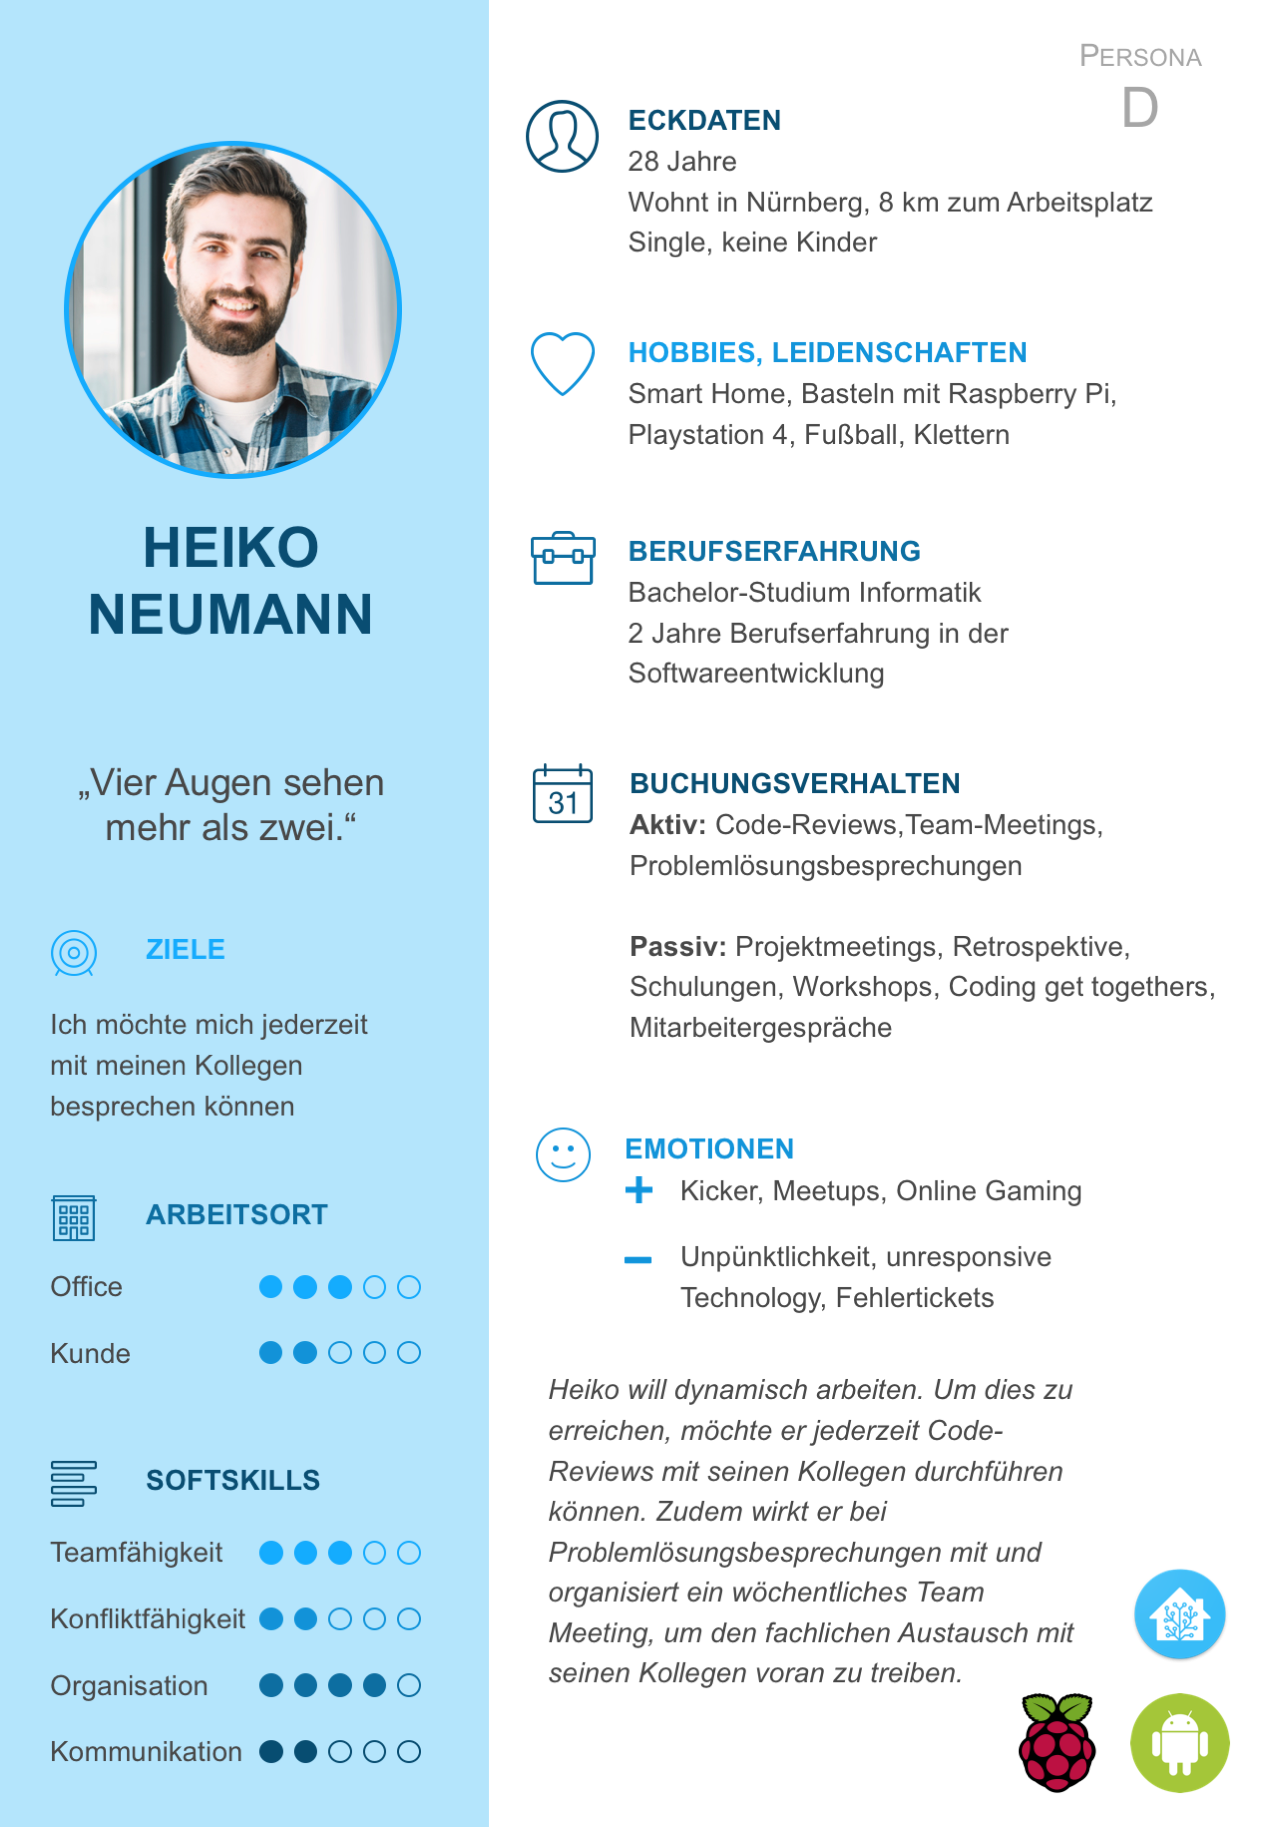
\includegraphics[width=0.9\textwidth]{bilder/anhang/Personae/PersonaD.png}}
    \caption{Persona Heiko Neumann aus dem Bereich \textit{Development}}
    \label{fig:persona-development}
\end{figure}

\begin{figure}[!htb]
    \centering
    \fbox{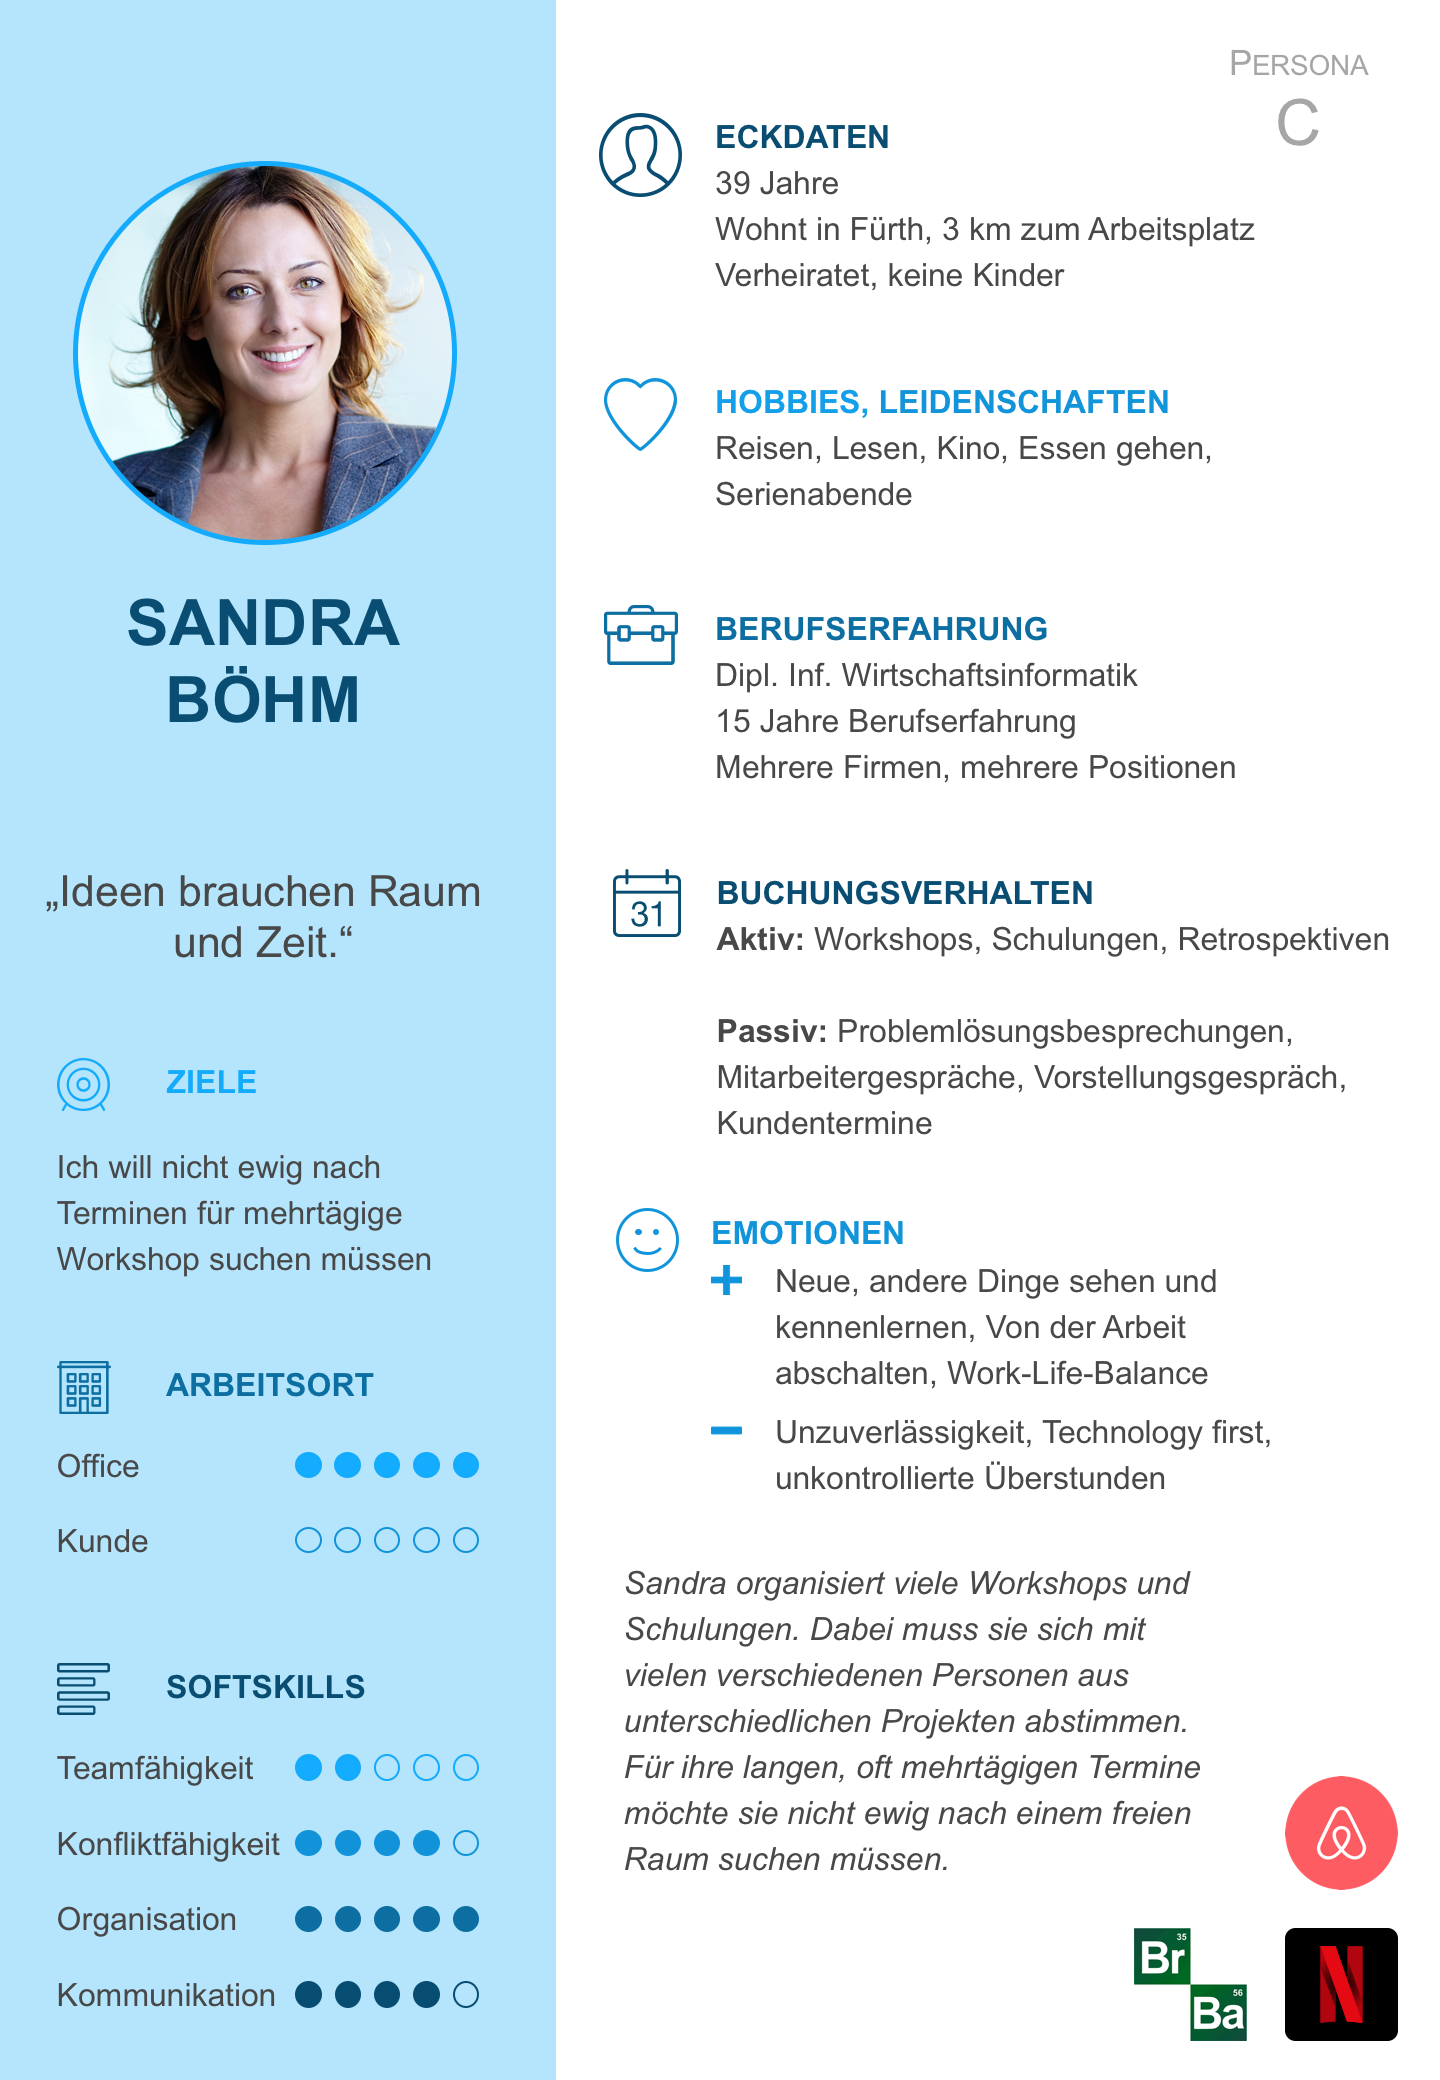
\includegraphics[width=0.9\textwidth]{bilder/anhang/Personae/PersonaC.png}}
    \caption{Persona Sandra Böhm aus dem Bereich \textit{Coaching}}
    \label{fig:persona-coaching}
\end{figure}

\begin{figure}[!htb]
    \centering
    \fbox{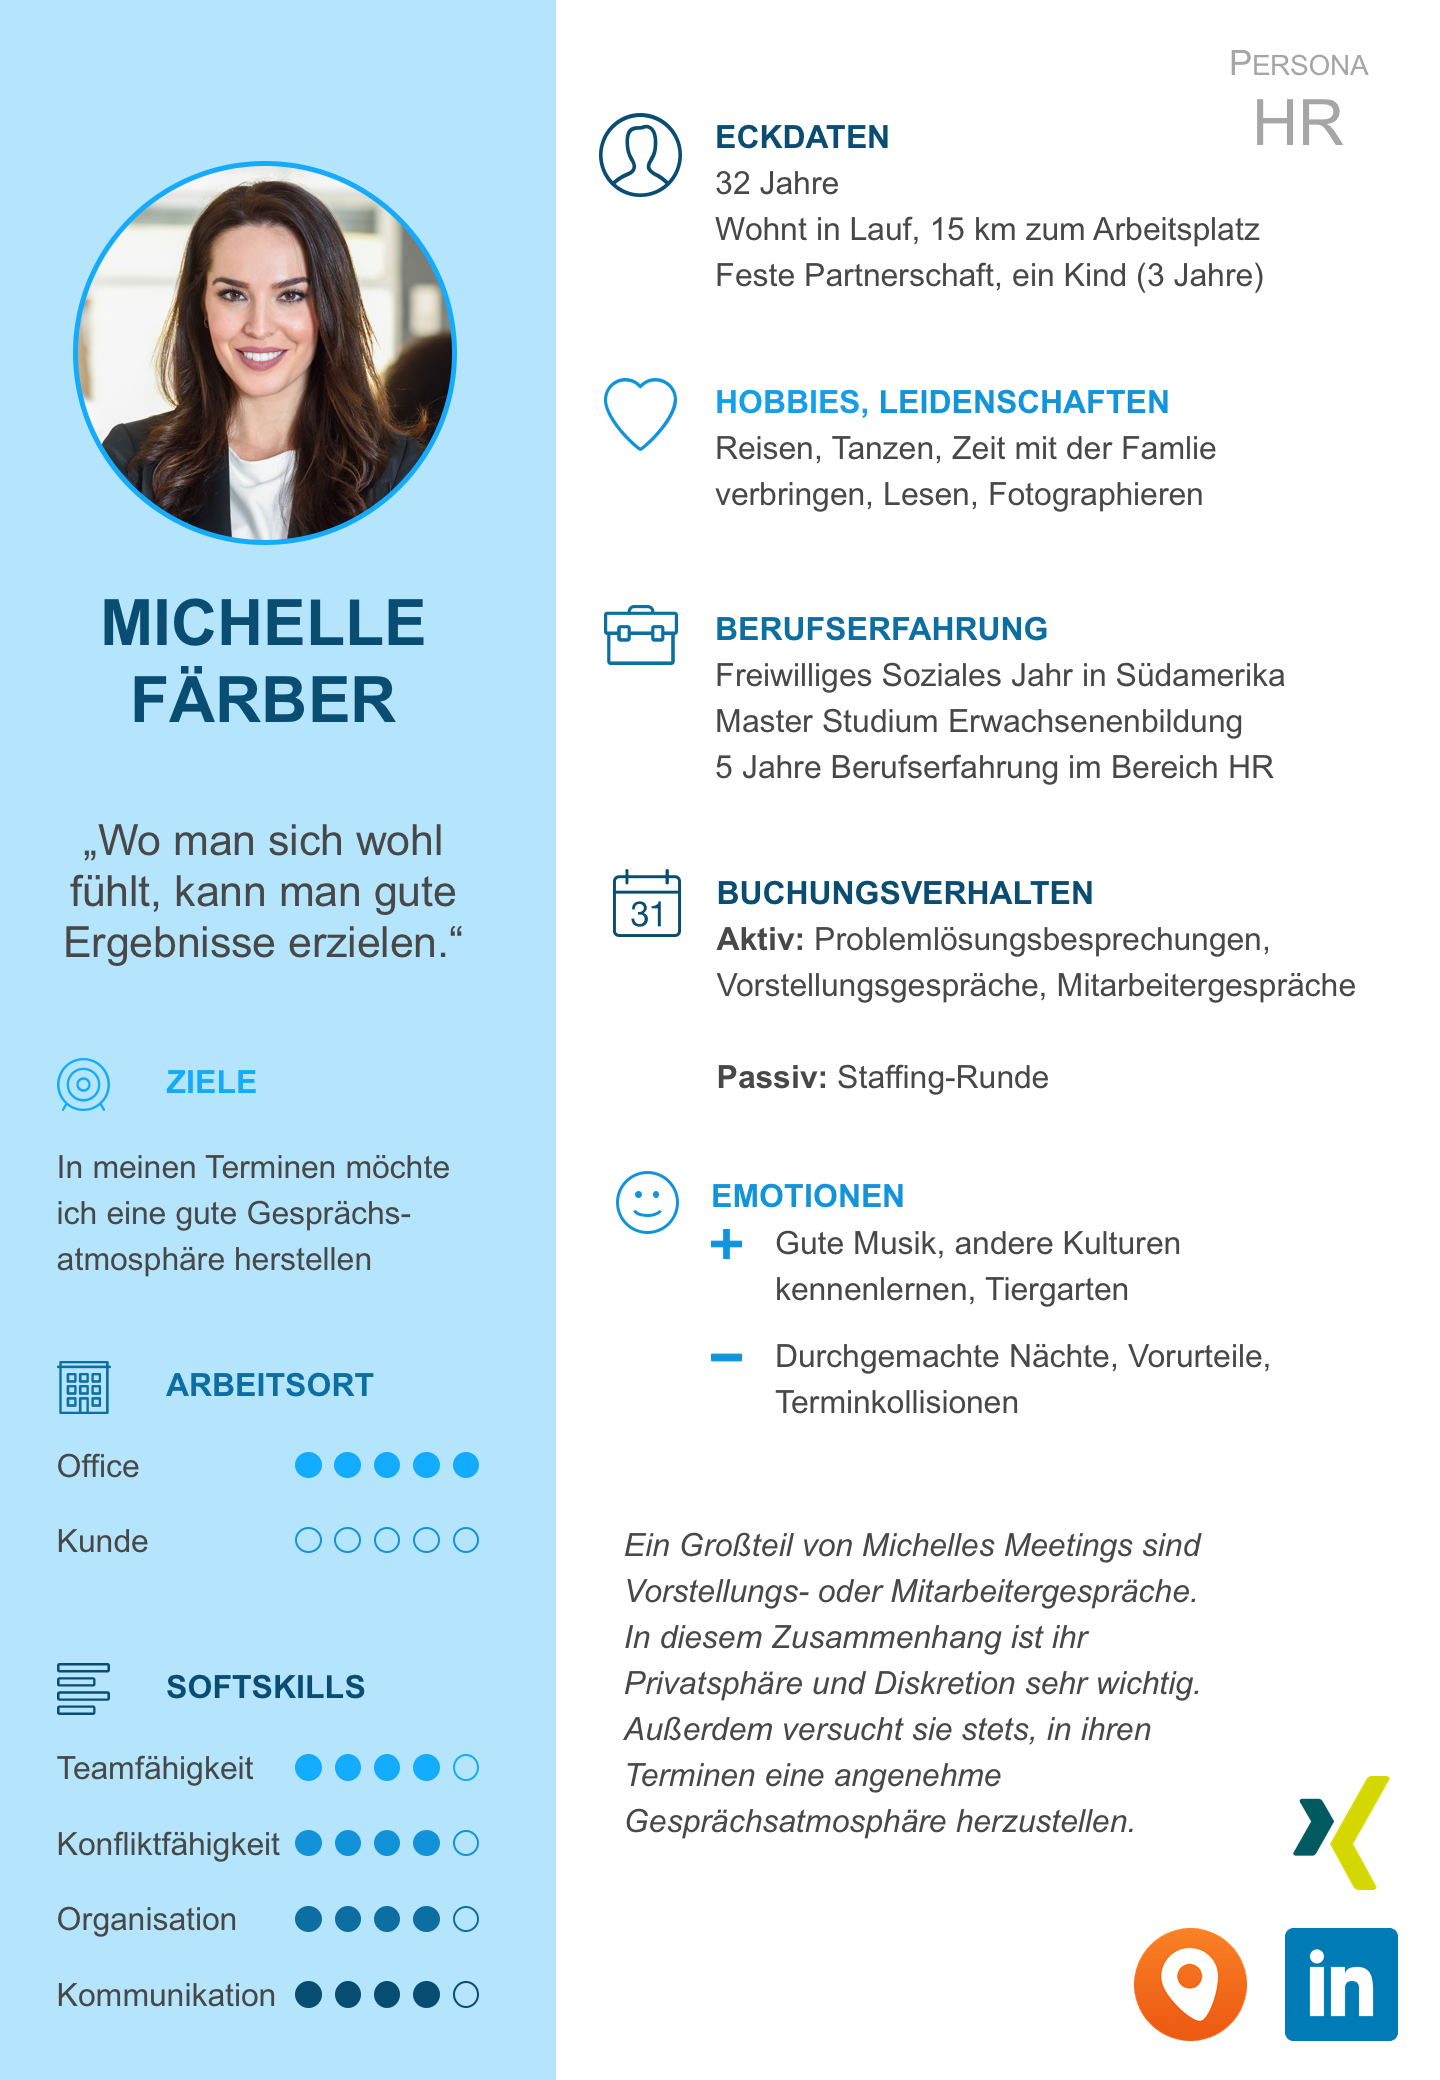
\includegraphics[width=0.9\textwidth]{bilder/anhang/Personae/PersonaHR.png}}
    \caption{Persona Michelle Färber aus dem Bereich \textit{Human Resources}}
    \label{fig:persona-human-resources}
\end{figure}

\begin{figure}[!htb]
    \centering
    \fbox{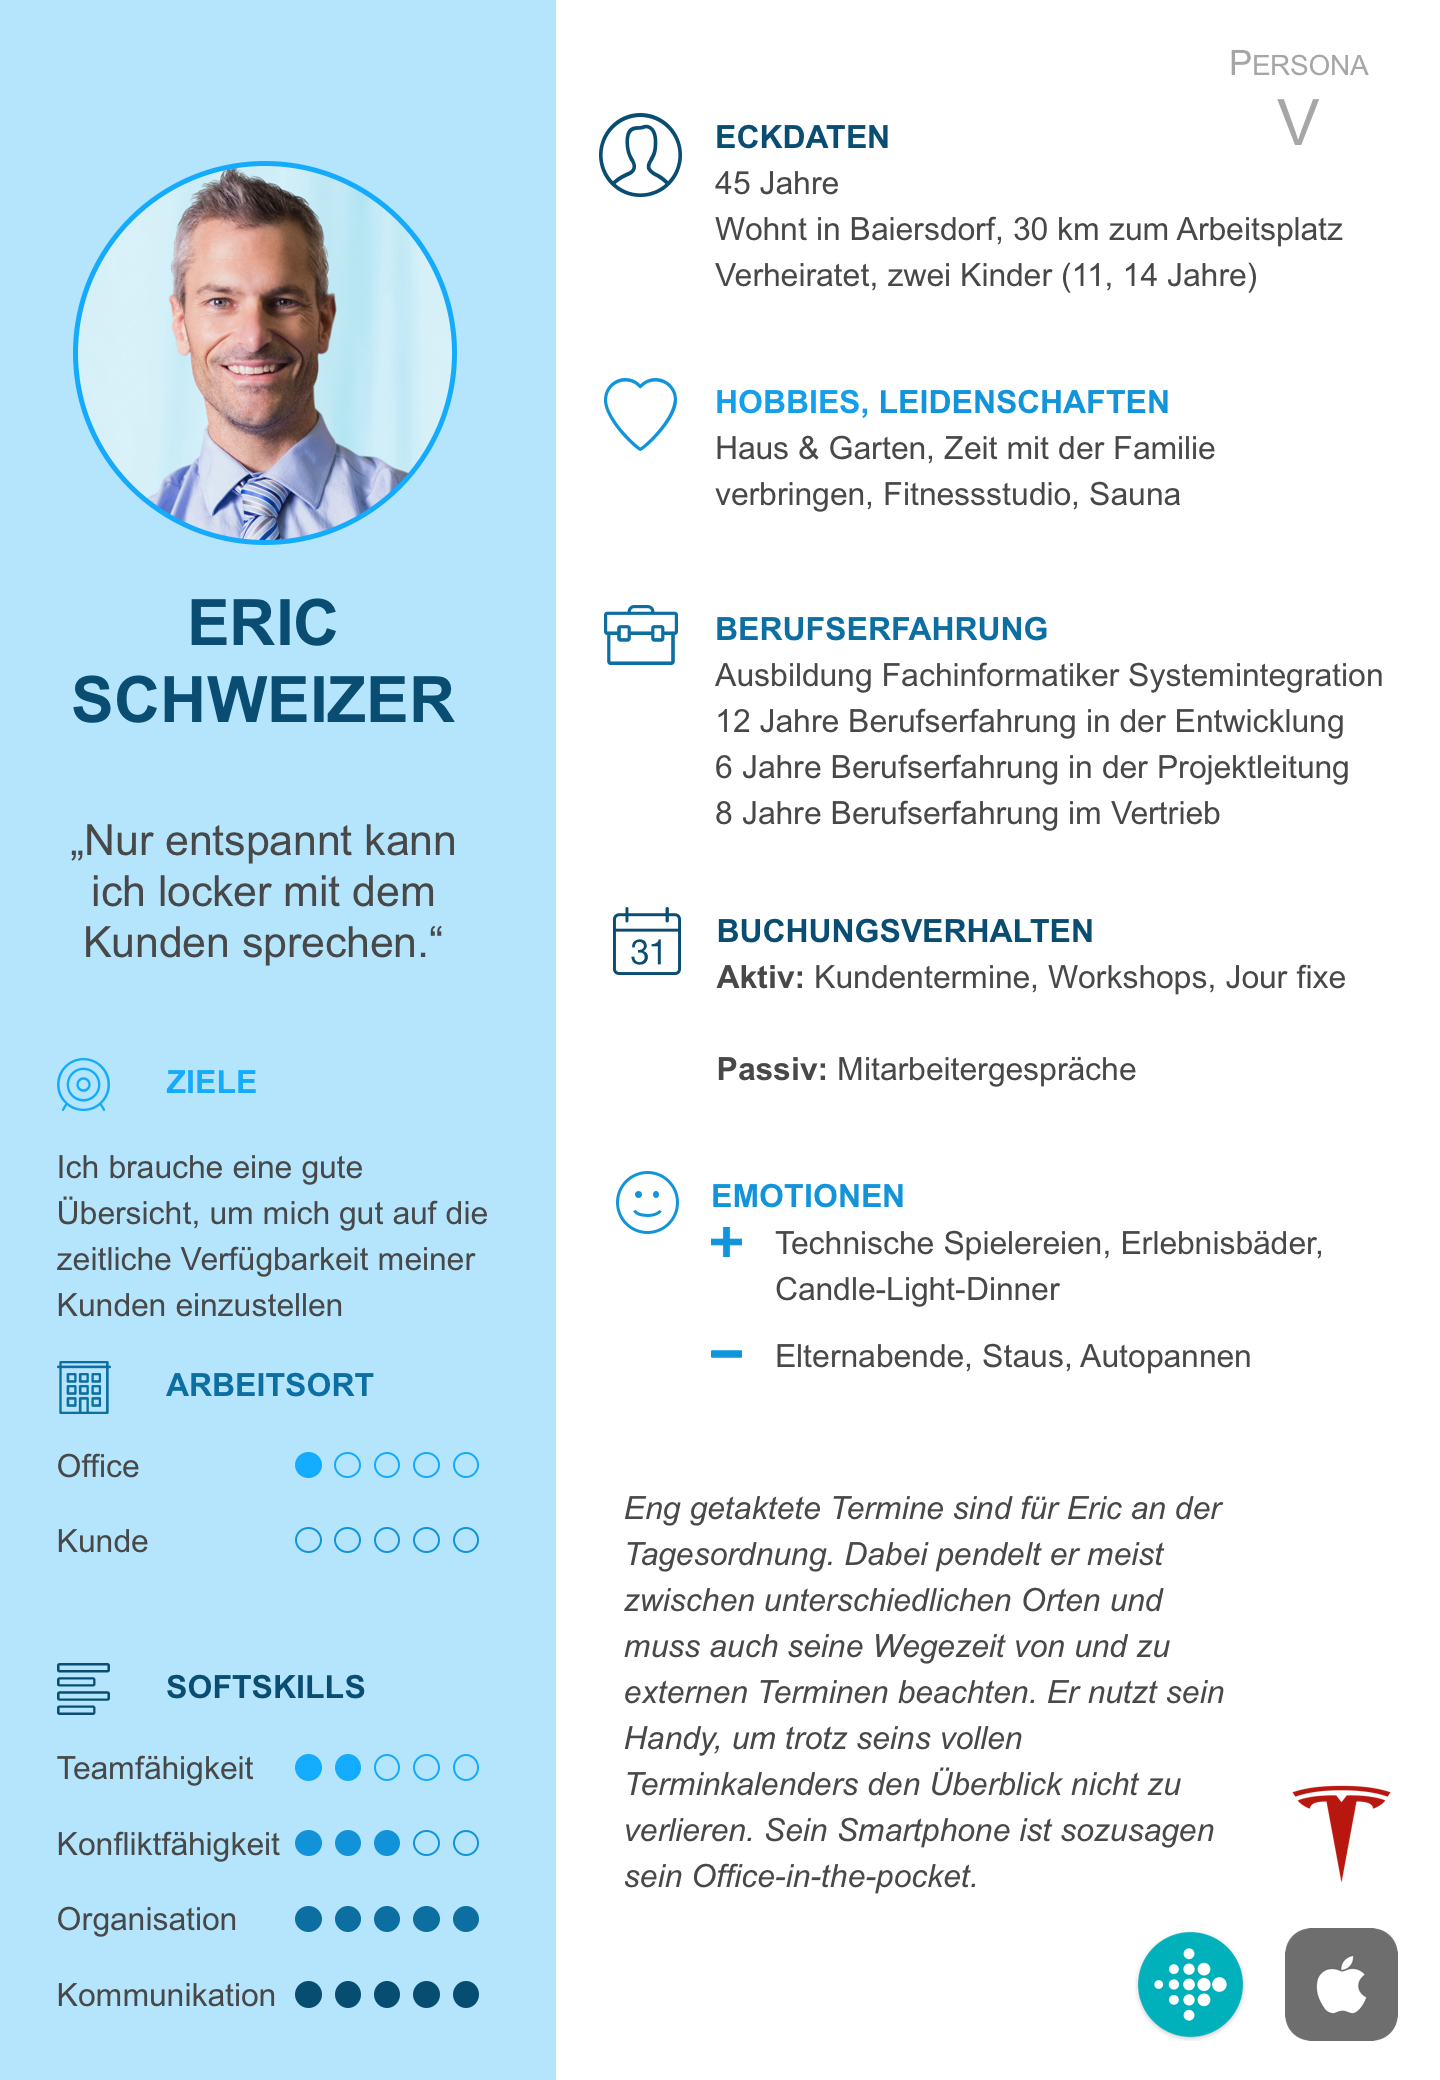
\includegraphics[width=0.9\textwidth]{bilder/anhang/Personae/PersonaV.png}}
    \caption{Persona Eric Schweizer aus dem Bereich \textit{Vertrieb}}
    \label{fig:persona-vertrieb}
\end{figure}

\clearpage

\section{\acs{UI}-Elemente aus dem Prototyping Tool}
\label{sec:anhang-ui-elemente-prototyping}

\begin{figure}[!htb]
    \centering
    \vspace{1.5cm}
    
\includegraphics[width=0.7\textwidth]{bilder/anhang/UIElementsPrototyping/TextMessage.png}
    \caption{\acs{UI}-Element \textit{TextMessage} aus dem Prototyping Tool}
    \label{fig:ui-element-textmessage}
\end{figure}

\begin{figure}[!htb]
    \centering
    \vspace{1.5cm}
    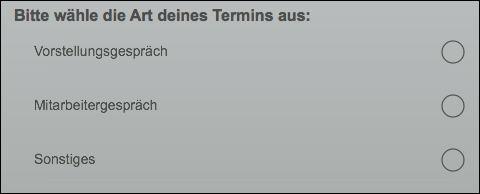
\includegraphics[width=0.7\textwidth]{bilder/anhang/UIElementsPrototyping/TypeOfMeeting.png}
    \caption{\acs{UI}-Element \textit{TypeOfMeeting} aus dem Prototyping Tool}
    \label{fig:ui-element-typeofmeeting}
\end{figure}

\begin{figure}[!htb]
    \centering
    \vspace{1.5cm}
    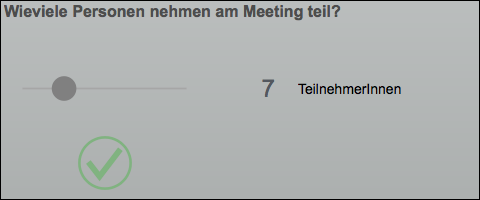
\includegraphics[width=0.7\textwidth]{bilder/anhang/UIElementsPrototyping/SliderParticipants.png}
    \caption{\acs{UI}-Element \textit{SliderParticipants} aus dem Prototyping Tool}
    \label{fig:ui-element-sliderparticipants}
\end{figure}

\begin{figure}[!htb]
    \centering
    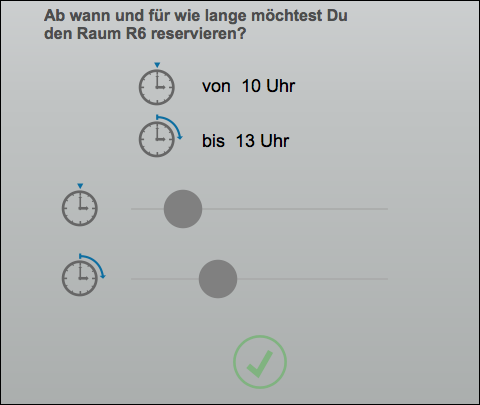
\includegraphics[width=0.6\textwidth]{bilder/anhang/UIElementsPrototyping/SliderStartEndTime.png}
    \caption{\acs{UI}-Element \textit{SliderStartEndTime} aus dem Prototyping Tool}
    \label{fig:ui-element-sliderstartendtime}
\end{figure}

\begin{figure}[!htb]
    \centering
    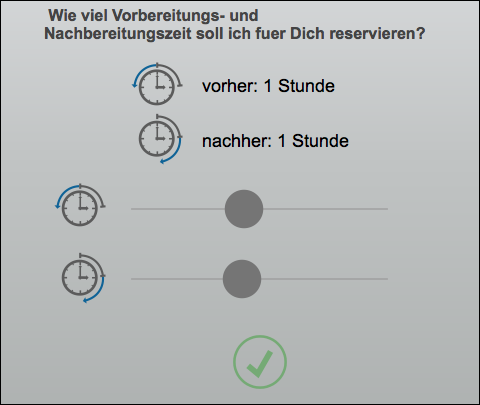
\includegraphics[width=0.6\textwidth]{bilder/anhang/UIElementsPrototyping/SliderTimeBuffer.png}
    \caption{\acs{UI}-Element \textit{SliderTimeBuffer} aus dem Prototyping Tool}
    \label{fig:ui-element-slidertimebuffer}
\end{figure}

\begin{figure}[!htb]
    \centering
    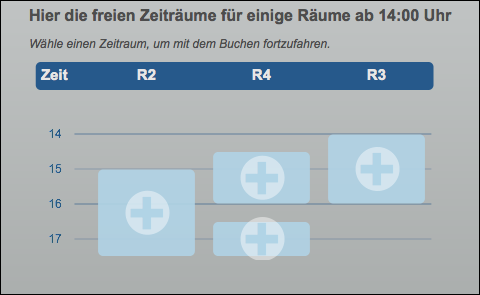
\includegraphics[width=0.7\textwidth]{bilder/anhang/UIElementsPrototyping/CalendarView.png}
    \caption{\acs{UI}-Element \textit{CalendarView} aus dem Prototyping Tool}
    \label{fig:ui-element-calendarview}
\end{figure}

\begin{figure}[!htb]
    \centering
    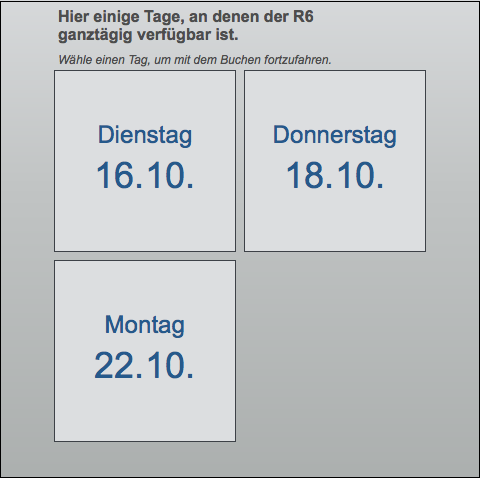
\includegraphics[width=0.6\textwidth]{bilder/anhang/UIElementsPrototyping/CollectionViewDates.png}
    \caption{\acs{UI}-Element \textit{CollectionViewDates} aus dem Prototyping Tool}
    \label{fig:ui-element-collectionviewdates}
\end{figure}

\begin{figure}[!htb]
    \centering
    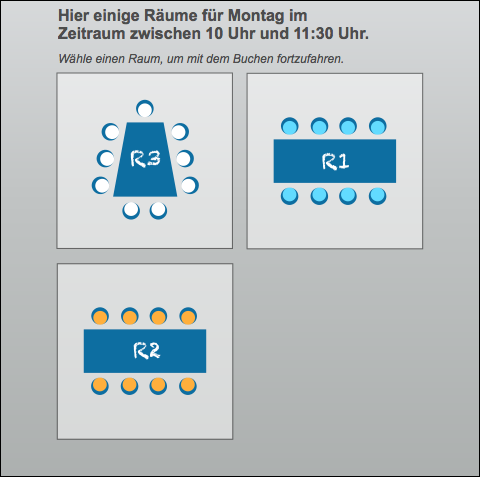
\includegraphics[width=0.6\textwidth]{bilder/anhang/UIElementsPrototyping/CollectionViewRooms.png}
    \caption{\acs{UI}-Element \textit{CollectionViewRooms} aus dem Prototyping Tool}
    \label{fig:ui-element-collectionviewrooms}
\end{figure}

\begin{figure}[!htb]
    \centering
    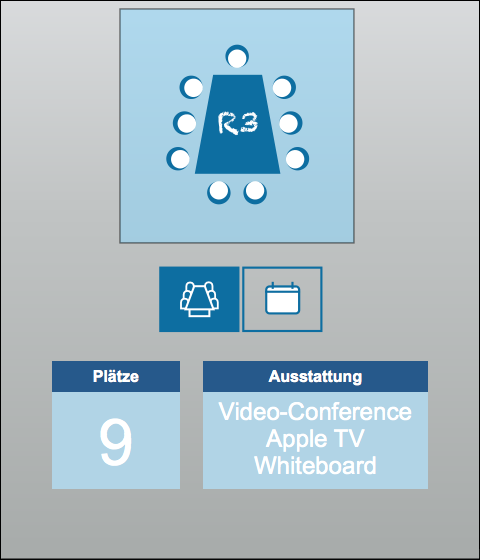
\includegraphics[width=0.6\textwidth]{bilder/anhang/UIElementsPrototyping/DetailView.png}
    \caption{\acs{UI}-Element \textit{DetailView} aus dem Prototyping Tool}
    \label{fig:ui-element-detailview}
\end{figure}

\begin{figure}[!htb]
    \centering
    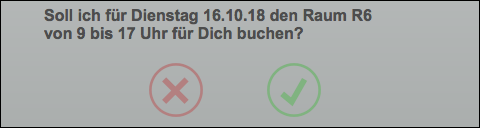
\includegraphics[width=0.7\textwidth]{bilder/anhang/UIElementsPrototyping/ConfirmBookingYesNo.png}
    \caption{\acs{UI}-Element \textit{ConfirmBooking} aus dem Prototyping Tool}
    \label{fig:ui-element-confirmbooking}
\end{figure}

\begin{figure}[!htb]
    \centering
    
\includegraphics[width=0.6\textwidth]{bilder/anhang/UIElementsPrototyping/Certificate.png}
    \caption{\acs{UI}-Element \textit{Certificate} aus dem Prototyping Tool}
    \label{fig:ui-element-certificate}
\end{figure}

\begin{figure}[!htb]
    \centering
    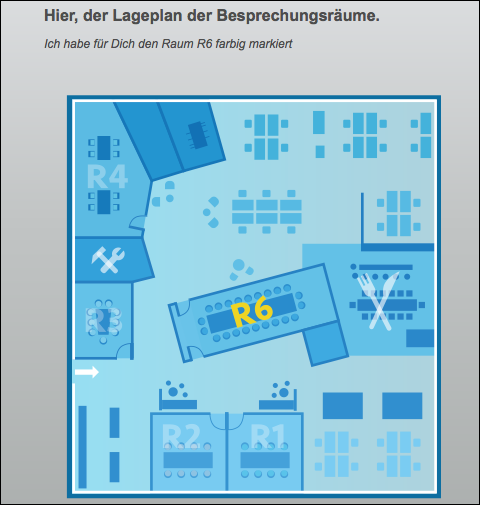
\includegraphics[width=0.6\textwidth]{bilder/anhang/UIElementsPrototyping/RoomMap.png}
    \caption{\acs{UI}-Element \textit{RoomMap} aus dem Prototyping Tool}
    \label{fig:ui-element-roommap}
\end{figure}

\section{Einverständniserklärung zum User Test}
\label{sec:anhang-einverstaendnis-user-test}

Die folgende Einverständniserklärung wird den Teilnehmern vor der Durchführung des
User Tests zur Unterschrift vorgelegt.

\textbf{Usability-Test zur Erfassung von Erfahrungen und Erwartungen in Hinblick auf die Nutzung eines Chatbots um einen Raum zu buchen}

Im Rahmen einer Masterarbeit an der Technischen Hochschule Nürnberg in Zusammenarbeit mit der \adorsys\ beschäftigen wir uns mit dem Design, der Bedienung und der Funktionalität eines Chatbots, mit dessen Hilfe Mitarbeiter und Mitarbeiterinnen einen Besprechungsraum reservieren können. Hierbei geht es um:

\begin{itemize}
\item die Benutzerführung für einen entsprechenden Chatbot
\item die Informationen, welche Nutzer von einem solchen Chatbot erwarten 
\item den Kommunikationsstil, den Nutzer erwarten
\end{itemize}

Hierfür führen wir einen Usability-Test mit einem von uns entwickelten Prototyping-Tool durch. Das Ziel ist es, mehr über Erwartungen von potentiellen Anwendern und die von ihnen verwendeten Formulierungen bei Nutzung eines Conversational Interfaces zu erfahren, und diese Erkenntnisse in die Entwicklung des Chatbots einfließen lassen zu können. 

Alle Fragen und Aufgaben in diesem Usability-Test beziehen sich auf die Einstufung und Verbesserung des Chatbots und nicht darauf, die Fähigkeiten und Fertigkeiten der Testperson zu testen. Alle Angaben werden vertraulich behandelt und ausschließlich anonymisiert verarbeitet und archiviert. Weiterhin werden diese Angaben nur im Rahmen der Entwicklung dieses Chatbots und in hierauf bezogene Präsentationen verwendet.

\begin{itemize}
\item Unternehmen: \adorsys\
\item Projektleitung: Steffen Blümm, Technical Lead iOS / CUI
\item Method: Think-Aloud
\item Dauer: 
\item Datum: 
\end{itemize}

\textbf{Einverständniserklärung}

Ich erkläre mich dazu bereit, im Rahmen des oben beschriebenen Projekts an einen Usability-Test teilzunehmen. Ich wurde über die Ziele des Projekts informiert. Ich kann den Test jederzeit abbrechen, weitere Tests ablehnen und meine Einwilligung in eine Aufzeichnung und Niederschrift des Tests jederzeit zurückziehen, ohne dass mir dadurch irgendwelche Nachteile entstehen.

Ich bin damit einverstanden, dass der Test mit einem Aufnahmegerät aufgezeichnet und sodann von den MitarbeiterInnen der adorsys ausgewertet wird. Für die Auswertung des Usability-Tests werden alle Angaben zu meiner Person aus dem Text entfernt und/oder anonymisiert. Mir wurde außerdem versichert, dass der Test in Veröffentlichungen nur in Ausschnitten zitiert wird, um sicherzustellen, dass ich auch durch die Reihenfolge von im Test erwähnten Ereignissen nicht für Dritte erkennbar sein werde. 
\\ \\ \\ \\ \\
Datum, Unterschrift der Testperson

\label{sec:anhang-einverstaendniserklaerung-feedback-ext}

\clearpage

\section{Feedback zum Usability Testessen}
\label{sec:anhang-feedback-ext}

\begin{figure}[!htb]
    \centering
    \fbox{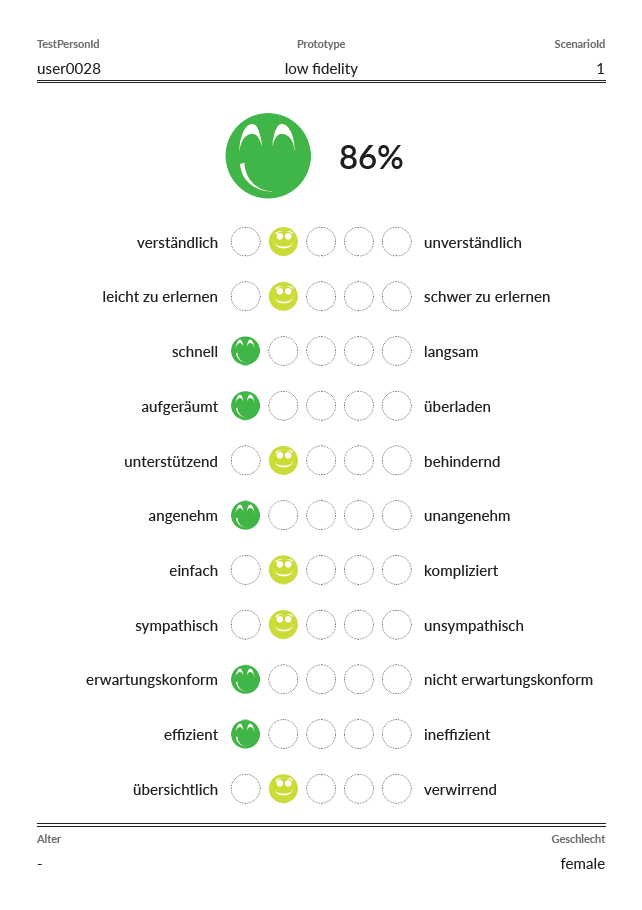
\includegraphics[width=0.9\textwidth]{bilder/anhang/UsabilityTestEssen/user0028-front.png}}
    \caption{Ergebnisse zum Fragebogen von user0028}
    \label{fig:feedback-user0028-front}
\end{figure}

\begin{figure}[!htb]
    \centering
    \fbox{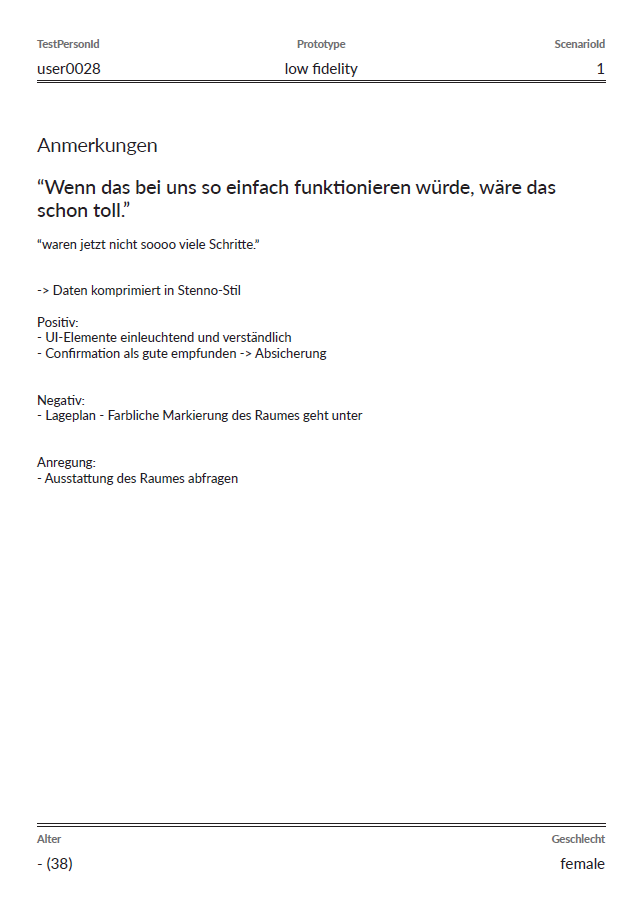
\includegraphics[width=0.9\textwidth]{bilder/anhang/UsabilityTestEssen/user0028-back.png}}
    \caption{Notizen zum Fragebogen von user0028}
    \label{fig:feedback-user0028-back}
\end{figure}

% new user

\begin{figure}[!htb]
    \centering
    \fbox{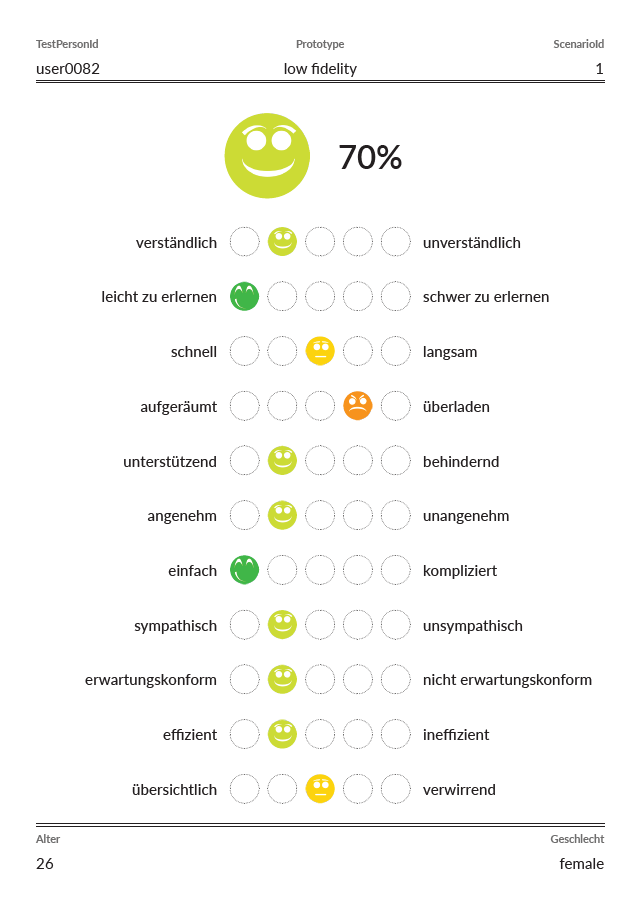
\includegraphics[width=0.9\textwidth]{bilder/anhang/UsabilityTestEssen/user0082-front.png}}
    \caption{Ergebnisse zum Fragebogen von user0082}
    \label{fig:feedback-user0082-front}
\end{figure}

\begin{figure}[!htb]
    \centering
    \fbox{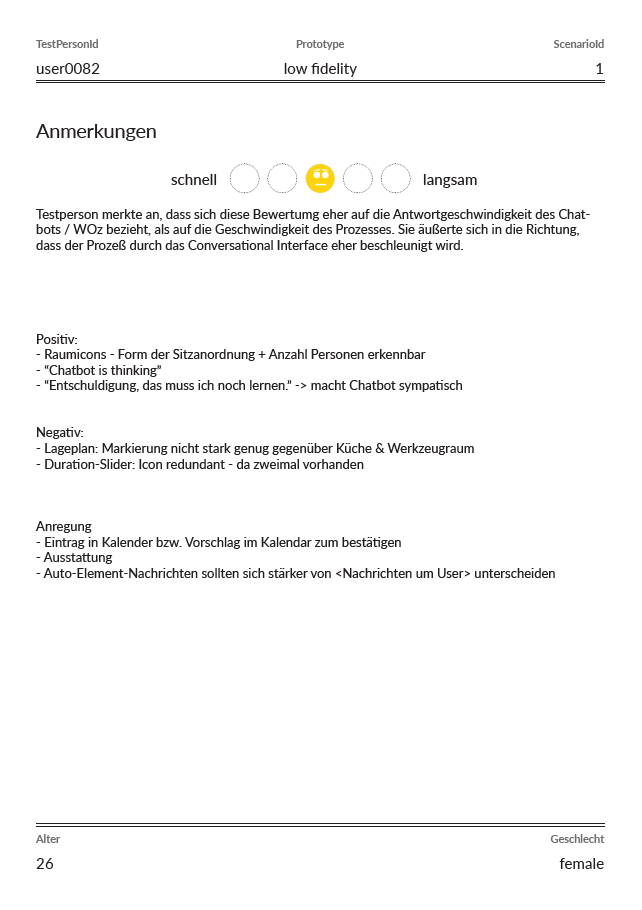
\includegraphics[width=0.9\textwidth]{bilder/anhang/UsabilityTestEssen/user0082-back.png}}
    \caption{Notizen zum Fragebogen von user0082}
    \label{fig:feedback-user0082-back}
\end{figure}

% new user

\begin{figure}[!htb]
    \centering
    \fbox{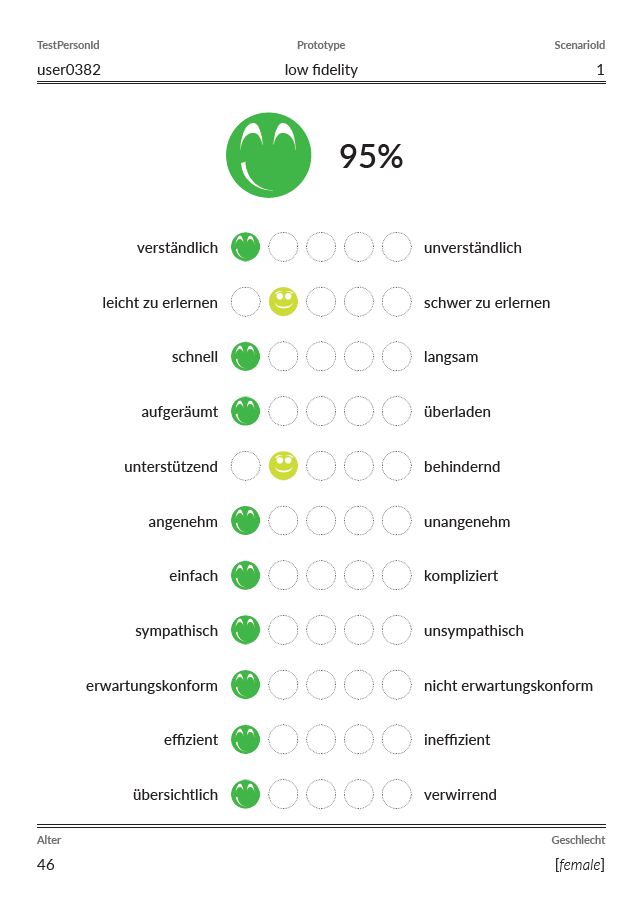
\includegraphics[width=0.9\textwidth]{bilder/anhang/UsabilityTestEssen/user0382-front.png}}
    \caption{Ergebnisse zum Fragebogen von user0382}
    \label{fig:feedback-user0382-front}
\end{figure}

\begin{figure}[!htb]
    \centering
    \fbox{\includegraphics[width=0.9\textwidth]{bilder/anhang/UsabilityTestEssen/user0382-back.png}}
    \caption{Notizen zum Fragebogen von user0382}
    \label{fig:feedback-user0382-back}
\end{figure}

% new user

\begin{figure}[!htb]
    \centering
    \fbox{\includegraphics[width=0.9\textwidth]{bilder/anhang/UsabilityTestEssen/user3729-front.png}}
    \caption{Ergebnisse zum Fragebogen von user3729}
    \label{fig:feedback-user3729-front}
\end{figure}

\begin{figure}[!htb]
    \centering
    \fbox{\includegraphics[width=0.9\textwidth]{bilder/anhang/UsabilityTestEssen/user3729-back.png}}
    \caption{Notizen zum Fragebogen von user3729}
    \label{fig:feedback-user3729-back}
\end{figure}

% new user

\begin{figure}[!htb]
    \centering
    \fbox{\includegraphics[width=0.9\textwidth]{bilder/anhang/UsabilityTestEssen/user5013-front.png}}
    \caption{Ergebnisse zum Fragebogen von user5013}
    \label{fig:feedback-user5013-front}
\end{figure}

\begin{figure}[!htb]
    \centering
    \fbox{\includegraphics[width=0.9\textwidth]{bilder/anhang/UsabilityTestEssen/user5013-back.png}}
    \caption{Notizen zum Fragebogen von user5013}
    \label{fig:feedback-user5013-back}
\end{figure}

% new user

\begin{figure}[!htb]
    \centering
    \fbox{\includegraphics[width=0.9\textwidth]{bilder/anhang/UsabilityTestEssen/user6271-front.png}}
    \caption{Ergebnisse zum Fragebogen von user6271}
    \label{fig:feedback-user6271-front}
\end{figure}

\begin{figure}[!htb]
    \centering
    \fbox{\includegraphics[width=0.9\textwidth]{bilder/anhang/UsabilityTestEssen/user6271-back.png}}
    \caption{Notizen zum Fragebogen von user6271}
    \label{fig:feedback-user6271-back}
\end{figure}

\clearpage

\section{Feedback zum User Test}
\label{sec:anhang-feedback-user-tests}

\begin{figure}[!htb]
    \centering
    \fbox{\includegraphics[width=0.9\textwidth]{bilder/anhang/UserTestAdorsys/user1723-front.png}}
    \caption{Ergebnisse zum Fragebogen von user1723}
    \label{fig:feedback-user1723-front}
\end{figure}

\begin{figure}[!htb]
    \centering
    \fbox{\includegraphics[width=0.9\textwidth]{bilder/anhang/UserTestAdorsys/user1723-back.png}}
    \caption{Notizen zum Fragebogen von user1723}
    \label{fig:feedback-user1723-back}
\end{figure}

% new user

\begin{figure}[!htb]
    \centering
    \fbox{\includegraphics[width=0.9\textwidth]{bilder/anhang/UserTestAdorsys/user2626-front.png}}
    \caption{Ergebnisse zum Fragebogen von user2626}
    \label{fig:feedback-user2626-front}
\end{figure}

\begin{figure}[!htb]
    \centering
    \fbox{\includegraphics[width=0.9\textwidth]{bilder/anhang/UserTestAdorsys/user2626-back.png}}
    \caption{Notizen zum Fragebogen von user2626}
    \label{fig:feedback-user2626-back}
\end{figure}

% new user

\begin{figure}[!htb]
    \centering
    \fbox{\includegraphics[width=0.9\textwidth]{bilder/anhang/UserTestAdorsys/user5156-front.png}}
    \caption{Ergebnisse zum Fragebogen von user5156}
    \label{fig:feedback-user5156-front}
\end{figure}

\begin{figure}[!htb]
    \centering
    \fbox{\includegraphics[width=0.9\textwidth]{bilder/anhang/UserTestAdorsys/user5156-back.png}}
    \caption{Notizen zum Fragebogen von user5156}
    \label{fig:feedback-user5156-back}
\end{figure}

% new user

\begin{figure}[!htb]
    \centering
    \fbox{\includegraphics[width=0.9\textwidth]{bilder/anhang/UserTestAdorsys/user7027-front.png}}
    \caption{Ergebnisse zum Fragebogen von user7027}
    \label{fig:feedback-user7027-front}
\end{figure}

\begin{figure}[!htb]
    \centering
    \fbox{\includegraphics[width=0.9\textwidth]{bilder/anhang/UserTestAdorsys/user7027-back.png}}
    \caption{Notizen zum Fragebogen von user7027}
    \label{fig:feedback-user7027-back}
\end{figure}

% new user

\begin{figure}[!htb]
    \centering
    \fbox{\includegraphics[width=0.9\textwidth]{bilder/anhang/UserTestAdorsys/user9337-front.png}}
    \caption{Ergebnisse zum Fragebogen von user9337}
    \label{fig:feedback-user9337-front}
\end{figure}

\begin{figure}[!htb]
    \centering
    \fbox{\includegraphics[width=0.9\textwidth]{bilder/anhang/UserTestAdorsys/user9337-back.png}}
    \caption{Notizen zum Fragebogen von user9337}
    \label{fig:feedback-user9337-back}
\end{figure}

% new user

\begin{figure}[!htb]
    \centering
    \fbox{\includegraphics[width=0.9\textwidth]{bilder/anhang/UserTestAdorsys/user9716-front.png}}
    \caption{Ergebnisse zum Fragebogen von user9716}
    \label{fig:feedback-user9716-front}
\end{figure}

\begin{figure}[!htb]
    \centering
    \fbox{\includegraphics[width=0.9\textwidth]{bilder/anhang/UserTestAdorsys/user9716-back.png}}
    \caption{Notizen zum Fragebogen von user9716}
    \label{fig:feedback-user9716-back}
\end{figure}

%%%%%%%%%% CD Verzeichnisstruktur %%%%%%%%%%

\clearpage

\section{CD Verzeichnisstruktur}
\label{sec:cd-verzeichnisstruktur}
\begin{tabbing}
	mm \= mm \= mmmmmmmmmmmmmmmm \= \kill
    $\vdash$ \textbf{Latex-Files/} $\Rightarrow$ \textit{editierbare \LaTeX~Dateien}\\ %\llcorner
	\> \>  $\vdash$  \textbf{bilder/}   	\> $\Rightarrow$ \textit{Alle verwendeten Bilder}\\
	\> \>  $\vdash$  \textbf{hauptkapitel/}  \> $\Rightarrow$ \textit{Fünf Hauptkapitel}\\
	\> \>  $\vdash$  \textbf{literatur/}   \> $\Rightarrow$ \textit{Bibliotheksdatei und Zitierstil}\\
	\> \>  $\vdash$  \textbf{nebenkapitel/}   \> $\Rightarrow$ \textit{Deckblatt, Abstract, Anhang, ...}\\
	\> \> --config.tex\\
	\> \> --main.tex\\
	|\\
	$\vdash$ \textbf{Literatur/} \\ 
	\> \>  $\vdash$  \textbf{Android/} \\
	\> \>  $\vdash$  \textbf{CUI/} \\ 
	\> \>  $\vdash$  \textbf{Server-Technologien/} \\ 
	\> \>  $\vdash$  \textbf{Usability/} \\ 
	|\\
	$\vdash$ \textbf{Quelltexte/} $\Rightarrow$\\ %\llcorner
	\> \>  $\vdash$  \textbf{AndroidApp/}   	\> $\Rightarrow$ \textit{Android Applikation}\\
	\> \>  $\vdash$  \textbf{Dialogflow/}   	\> $\Rightarrow$ \textit{Dialogflow Agent}\\
	\> \>  $\vdash$  \textbf{PrototypingTool/}   	\> $\Rightarrow$ \textit{\ac{JSON}-Files der Szenarien}\\
	\> \>  $\vdash$  \textbf{Server/}   	\> $\Rightarrow$ \textit{Node.js Webservice}\\
    |\\
    $\vdash$ \textbf{Weiteres/} \\
    \> \>  $\vdash$  \textbf{AppVideos/}   	\> $\Rightarrow$ \textit{Beispielvideos zur Android Applikation}\\
	\> \>  $\vdash$  \textbf{Dokumente/}   	\> $\Rightarrow$ \textit{Exposee, Masterarbeit, Praesentation}\\
	|\\
\end{tabbing}
\end{appendix}

\end{document}
